\documentclass[a5paper,9pt,final]{extarticle}
\usepackage[top=1cm,bottom=2cm,left=1cm,right=1cm]{geometry}

\usepackage{amsmath}
\usepackage{amssymb}
\usepackage{amsthm}
\usepackage{listings}
\usepackage{color}
%\usepackage{verbatim}
\usepackage{graphicx}
\usepackage{wrapfig}
\usepackage{subcaption}
\usepackage{tabularx}
    \usepackage{multirow}
\usepackage{slashbox}
\usepackage{bm}

\usepackage[multiple]{footmisc}


\usepackage{hyperref}
\hypersetup{
    linktoc=all,     %set to all if you want both sections and subsections linked
}

\usepackage{tikz}

% \linespread{1.62}
\sloppy
 
\usepackage{xltxtra}
\setmainfont[
Mapping=tex-text,
BoldItalicFont=GHEAGrapalatBlit.otf,
BoldFont      =GHEAGpalatBld.otf,
ItalicFont    =GHEAGrapalatRit.otf]{GHEAGrpalatReg.otf}

\renewcommand\figurename{Նկ.}
\renewcommand\tablename{Աղյուսակ}
\renewcommand\refname{Գրականություն}
\renewcommand\contentsname{Բովանդակություն}

\usepackage{titlesec}
\titlespacing*{\section}{0pt}{0.7cm}{0.5cm}

\title{Գրաֆների միջակայքային կողային ներկումների հետազոտում}
\date{}
\newtheorem{theorem}{Թեորեմ}[subsection]
\newtheorem{lemma}[theorem]{Լեմմա}
\newtheorem{corollary}[theorem]{Հետևանք}
\newtheorem{remark}[theorem]{Պնդում}
\newtheorem{definition}{Սահմանում}%[section]
\newtheorem{hypothesis}{Հիպոթեզ}[section]
\newtheorem{problem}{Խնդիր}[section]

\usepackage{chngcntr}
\counterwithin{figure}{section}
\counterwithin{table}{section}

% \let\stdsection\section
% \renewcommand\section{\newpage\stdsection}

\DeclareMathOperator{\sign}{sgn}


% \DeclareUnicodeCharacter{00A0}{ }

\usepackage{environ}
\NewEnviron{killcontents}{}
\let\proof\killcontents
\let\endproof\endkillcontents

\newenvironment{hide}%
  {\renewcommand\section[1]{\refstepcounter{section}}%
   \renewcommand\subsection[1]{\refstepcounter{subsection}}%
   \RenewEnviron{theorem}{\refstepcounter{theorem}}
   \RenewEnviron{lemma}{\refstepcounter{theorem}}
   \RenewEnviron{remark}{\refstepcounter{theorem}}
   \RenewEnviron{corollary}{\refstepcounter{theorem}}
   \RenewEnviron{hypothesis}{\refstepcounter{hypothesis}}
   \RenewEnviron{figure}{\refstepcounter{figure}}
   \RenewEnviron{table}{\refstepcounter{table}}
  }%
  {}
\begin{document}

\thispagestyle{empty}
\begin{center}

\textsc{ԵՐԵՎԱՆԻ ՊԵՏԱԿԱՆ ՀԱՄԱԼՍԱՐԱՆ}\\[1cm]

{Խաչատրյան Հրանտ Հարությունի\\[0.5cm]}
{Գրաֆների միջակայքային կողային ներկումների հետազոտում\\[1.2cm]}
{ՍԵՂՄԱԳԻՐ \\[1.2cm]}

Ա.01.09 «Մաթեմատիկական կիբեռնետիկա և  
մաթեմատիկական \\ տրամաբանություն» մասնագիտությամբ ֆիզիկամաթեմատիկական \\ գիտությունների թեկնածուի գիտական աստիճանի հայցման ատենախոսության \\[1cm]

Երևան - 2017\\[0.6cm]
\rule{\textwidth}{1pt}\\[0.8cm]

\textsc{ЕРЕВАНСКИЙ ГОСУДАРСТВЕННЫЙ УНИВЕРСИТЕТ}\\[1cm]

{Xaчатрян Грант Арутюнович\\[0.5cm]}
{Исследование интервальных реберных раскрасок графов\\[1.2cm]}
{АВТОРЕФЕРАТ \\[1.2cm]}

диссертации на соискание ученой степени кандидата \\
физико-математических наук по специальности\\ 01.01.09 “Математическая кибернетика и математическая логика” \\[1cm]
\vfill

Ереван - 2017\\[0.2cm]


\end{center}

Ատենախոսության թեման հաստատվել է Երևանի պետական համալսարանում:\\[0.3cm]

\begin{tabularx}{\textwidth}{Xl}
Գիտական ղեկավար՝     & ֆիզ.-մաթ. գիտ. թեկնածու Պ. Ա. Պետրոսյան \\
Պաշտոնական ընդդիմախոսներ՝ & ֆիզ.-մաթ. գիտ. դոկտոր Է. Մ. Պողոսյան \\
 & ֆիզ.-մաթ. գիտ. թեկնածու Հ. Ց. Հակոբյան \\
Առաջատար կազմակերպություն՝  & Հայ-ռուսական (սլավոնական) համալսարան
\end{tabularx}\\[0.5cm]
     
Պաշտպանությունը կայանալու է 2017թ. հունիսի 9-ին, ժ. 14\textsuperscript{30}-ին ԵՊՀ-ում գործող ԲՈՀ-ի 044 «Մաթեմատիկական կիբեռնետիկա» մասնագիտական խորհրդի նիստում հետևյալ հասցեով՝ 0025, Երևան, Ալ. Մանուկյան 1:\\[0.5cm]  
Ատենախոսությանը կարելի է ծանոթանալ ԵՊՀ-ի գրադարանում: \\[0.5cm]
Սեղմագիրն առաքված է 2017թ. մայիսի 6-ին:\\[0.5cm]
\begin{tabularx}{\textwidth}{Xlr}
Մասնագիտական խորհրդի  & \multirow{3}{*}{\includegraphics[width=0.1\textwidth]{figures/dumanyan.pdf}\hspace{1cm}} &                \\
գիտական քարտուղար,    &                                                                                    &                \\
ֆիզ.-մաթ.գիտ. դոկտոր՝ &                                                                                    & Վ.Ժ. Դումանյան
\end{tabularx}\\[0.5cm]

\rule{\textwidth}{1pt}\\[0.4cm]

Тема диссертации утверждена в Ереванском государственном университете.\\[0.3cm]

\begin{tabularx}{\textwidth}{Xl}
Научный руководитель:     & кандидат физ.-мат. наук П. А. Петросян \\
Официальные оппоненты:  & доктор физ.-мат. наук Э. М. Погосян \\
 & кандидат физ.-мат. наук Г. Ц. Акопян \\
Ведущая организация:  & Российско-Армянский (Славянский) университет
\end{tabularx}\\[0.5cm]
                          
Защита состоится 9-го июня 2017г. в 14\textsuperscript{30} часов на заседании действующего в Ереванском государственном университете специализированного совета ВАК 044
“Математическая кибернетика”, по адресу: Ереван 0025, ул. А. Манукяна, 1.\\[0.5cm]
С диссертацией можно ознакомиться в библиотеке Ереванского государственного университета.\\[0.5cm]
Автореферат разослан 6-го мая 2017г. \\[0.5cm]

\begin{tabularx}{\textwidth}{Xlr}
Ученый секретарь  & \multirow{3}{*}{\includegraphics[width=0.1\textwidth]{figures/dumanyan.pdf}\hspace{1cm}} &                \\
специализированного  совета,    &                                                                                    &                \\
доктор физ.-мат. наук &                                                                                    & В.Ж. Думанян
\end{tabularx}


\pagebreak
\section*{Աշխատանքի ընդհանուր նկարագիրը}\
\paragraph{Թեմայի արդիականությունը:} 

Դիսկրետ մաթեմատիկայում մեծ ուշադրություն է հատկացվում ներկումների խնդիրների հետազոտություններին: Պատմականորեն ներկումների հանդեպ հետաքրքրությունը պայմանավորված էր «Չորս գույների հիպոթեզ» հանրահայտ խնդրով, համաձայն որի ամեն մի աշխարհագրական քարտեզ հնարավոր է ներկել չորս գույների միջոցով այնպես, որ յուրաքանչյուր երկրի տարածք ներկված լինի մեկ գույնով, իսկ ընդհանուր սահման ունեցող երկրները ներկված լինեն տարբեր գույներով: Դիսկրետ մաթեմատիկայի հետագա զարգացումը ցույց տվեց, որ դա պայմանավորված է ինչպես ներկումների խնդիրների՝ մի շարք կարևոր կիրառական խնդիրների հետ առկա սերտ կապով, այնպես էլ նրանով, որ դիսկրետ մաթեմատիկայում առկա են բազմաթիվ խնդիրներ, որոնք կարելի է ձևակերպել որպես ներկումների խնդիրներ (ֆակտորիզացիայի խնդիրներ, տրոհման խնդիրներ, Ռամսեյի տեսության խնդիրներ և այլն): Մասնավորապես, նշանակալի փոխադարձ կապ կա կարգացուցակների տեսության խնդիրների և գրաֆների ներկումների խնդիրների միջև: Օրինակ, քննաշրջանի օպտիմալ կարգացուցակ կառուցելու խնդիրը բերվում է գրաֆի քրոմատիկ թվի որոշմանը: Գրաֆի քրոմատիկ դասը գտնելու խնդրին բերվում է սպորտային մրցումների կարգացուցակ կազմելու խնդիրը:

Կարգացուցակների տեսության բազմաթիվ խնդիրներ կարելի է բերել ոչ միայն գրաֆների դասական ներկումների խնդիրներին, այլև լրացուցիչ պայմաններով ճիշտ գագաթային և կողային ներկումների գոյության ու կառուցման խնդիրներին: Օրինակ, Ջ. Ֆոլկմանը և Դ. Ֆալկերսոնը\footnote{J. Folkman, D.R. Fulkerson, Edge colourings in bipartite graphs, in Combinatorial  Mathematics and its Applications, University of North Carolina Press, Chapel Hill, 1969, pp. 561-577.} դիտարկել են երկկողմանի մուլտիգրաֆը $r$ գույներով ճիշտ կողային ներկման գոյության խնդիրը, երբ $i$ գույնով ներկված կողերի քանակը $n_i$ է, $i=1,\ldots,r$: Այս խնդիրը համապատասխանում է $r$ ժամ ընդհանուր տևողություն ունեցող այնպիսի ուսումնական դասացուցակի կառուցմանը, երբ $i$-րդ ժամի ընթացքում զբաղված է ճիշտ $n_i$ լսարան, $i=1,\ldots,r$: Իվենի, Իտայի և Շամիրի կողմից\footnote{S. Even, A. Itai, A. Shamir, On the complexity of timetable and multicommodity flow problems, SIAM J. Comput. 5 (4), 1976, pp. 691-703.} դիտարկվել է այնպիսի ուսումնական դասացուցակների կառուցումը, որտեղ հաշվի են առնվում ուսուցիչների նախապատվությունները: Ցույց է տրվել, որ ընդհանուր դեպքում խնդիրը NP-լրիվ է: Գրաֆների տեսության տերմիններով այս խնդիրը համապատասխանում է $G$ երկկողմանի մուլտիգրաֆի այնպիսի ճիշտ կողային ներկման կառուցմանը, որտեղ $G$-ի կողմերից մեկի յուրաքանչյուր գագաթի համար տրված են գույների բազմություններ, որոնցից պետք է ընտրվեն այդ գագաթին կից կողերի գույները: Դե Վերրայի կողմից\footnote{D. de Werra, Balanced schedules, INFOR. N9, 1971, pp. 230-237.} դիտարկվել են երկկողմանի մուլտիգրաֆների կողային ներկումների գոյության և կառուցման խնդիրները, երբ յուրաքանչյուր գագաթի համար այդ գագաթին կից ցանկացած երկու գույնով ներկված կողերի քանակների տարբերությունը մեծ չէ մեկից: Ցույց է տրվել, որ կամայական $G$ երկկողմանի մուլտիգրաֆի և $k$ բնական թվի համար $G$-ի կողերը կարելի է ներկել $k$ գույներով՝ բավարարելով նշված պայմանին: Այս խնդիրը համապատասխանում է այնպիսի դասացուցակներին, երբ ուսուցիչների և դասարանների ծանրաբեռնվածությունները բաշխվում են հավասարաչափ: «Պատուհան» չունեցող դասացուցակների գոյության և կառուցման խնդիրներին համապատասխանող գրաֆների ներկումների խնդիրների հետազոտման նպատակով Ա. Հասրաթյանի և Ռ. Քամալյանի կողմից\footnote{ А.С. Асратян, Р.Р. Камалян, Интервальные раскраски ребер мультиграфа, Прикладная математика, вып. 5, 1987, стр. 25-34.} սահմանվել է գրաֆի միջակայքային կողային ներկման գաղափարը: $G$ գրաֆի ճիշտ կողային ներկումը $1,\ldots,t$ գույներով կոչվում է $G$-ի միջակայքային կողային $t$-ներկում, եթե յուրաքանչյուր գագաթին կից կողերը ներկված են հաջորդական գույներով: Մի շարք աշխատանքներում հետազոտվել են երկկողմանի գրաֆների որոշ դասերի միջակայքային կողային ներկումները, որոնցից են լրիվ երկկողմանի գրաֆները, ծառերը, $n$-չափանի խորանարդը, ցանցերը, երկակի ուռուցիկ երկկողմանի գրաֆները, արտաքին հարթ երկկողմանի գրաֆները և $(a,b)$-երկհամասեռ երկկողմանի գրաֆները: Հայտնի է, որ ոչ բոլոր երկկողմանի գրաֆները ունեն միջակայքային կողային ներկում: Այդ փաստը առաջին անգամ նշվել է Ա. Միրումյանի կողմից: Հետագայում այդպիսի օրինակներ կառուցվել են Ս. Սեվաստյանովի, Պ. Էրդյոշի, Ա. Հերցի, Դ. դե Վերրայի, Կ. Գիարոյի, Մ. Կուբալի և Մ. Մալաֆիյսկու, ինչպես նաև Քամալյանի կողմից: Սեվաստյանովը ապացուցել է, որ երկկողմանի գրաֆների դասում միջակայքային կողային ներկման գոյության խնդիրը հանդիսանում է NP-լրիվ խնդիր\footnote{С.В. Севастьянов, Об интервальной раскрашиваемости ребер двудольного графа, Методы дискретного анализа в решении экстремальных задач, вып. 50, 1990, стр. 61-72.}: Նշենք նաև, որ Ջենսենի և Տոֆտի կողմից\footnote{T.R. Jensen, B. Toft, Graph coloring problems, Wiley Interscience Series in Discrete Mathematics and Optimization, 1995.} առաջարկվել է հիպոթեզ, համաձայն որի բոլոր $(a,b)$-երկհամասեռ երկկողմանի գրաֆները ունեն միջակայքային կողային ներկում: Այս հիպոթեզի ապացույցի ուղղությամբ Ա. Հասրաթյանը, Կ. Կասսելգրենը, Պ. Պետրոսյանը, Ջ. Վանդենբուշեն, Դ. Վեստը, Ա. Պյատկինը, Բ. Տոֆտը, Ֆ. Յանգը և Ք. Լին հասել են որոշ հաջողությունների:

Կիրառական խնդիրների մոդելավորման ժամանակ հաճախ հետազոտման օբյեկտներ են հանդիսանում ոչ միայն հասարակ գրաֆները, այլև մուլտիգրաֆները: Այսպես, օրինակ, ուսումնական դասացուցակների կառուցման խնդիրներում հաճախ առաջանում են իրավիճակներ, երբ ուսուցիչը միևնույն խմբի հետ անցկացնում է մեկից ավելի դասաժամ: Միջակայքային կողային ներկումներին նվիրված հետազոտությունները վերջին երեք տասնամյակներում հիմնականում վերաբերում էին պատիկ կողեր չպարունակող գրաֆներին, մինչդեռ մուլտիգրաֆները մնում են քիչ հետազոտված: Մյուս կողմից՝ վերոհիշյալ աշխատանքներում հիմնականում ուսումնասիրվել են միջակայքային ներկումների գոյության և կառուցման խնդիրները, սակայն քիչ է անդրադարձ կատարվել ներկումների թվային պարամետրերի գնահատման հարցերին: Միջակայքային ներկումների հետազոտություններում անարդարացիորեն քիչ է ուշադրություն հատկացված այդպիսի ներկումների կայունության հարցերին տարբեր գրաֆային գործողությունների նկատմամբ, ինչպիսիք են, օրինակ, գրաֆների գումարումը, դեկարտյան արտադրյալը, գրաֆից գագաթների, կողերի կամ զուգակցումների հեռացումը, կողերի տրոհումը և այլն: Նման դրվածքով խնդիրների կարևորությունը հատկապես մեծ է այնպիսի համակարգերի մոդելավորման դեպքում, որոնցում ժամանակի ազդեցության տակ կարող են կատարվել նկարագրող գրաֆի (մուլտիգրաֆի) չնախատեսված փոփոխություններ:

% Դիսկրետ մաթեմատիկայում մեծ ուշադրություն է հատկացվում ներկումների խնդիրների հետազոտություններին: Դա պայմանավորված է ինչպես ներկումների խնդիրների՝ մի շարք կարևոր կիրառական խնդիրների հետ առկա սերտ կապով, այնպես էլ նրանով, որ դիսկրետ մաթեմատիկայում առկա են բազմաթիվ խնդիրներ, որոնք կարելի է ձևակերպել որպես ներկումների խնդիրներ (ֆակտորիզացիայի խնդիրներ, տրոհման խնդիրներ, Ռամսեյի տեսության խնդիրներ և այլն): Մասնավորապես, նշանակալի փոխադարձ կապ կա կարգացուցակների տեսության խնդիրների և գրաֆների ներկումների խնդիրների միջև: Օրինակ, քննաշրջանի օպտիմալ կարգացուցակ կառուցելու խնդիրը բերվում է գրաֆի քրոմատիկ թվի որոշմանը: Գրաֆի քրոմատիկ դասը գտնելու խնդրին բերվում է սպորտային մրցումների կարգացուցակ կազմելու խնդիրը:

% «Պատուհան» չունեցող դասացուցակների գոյության և կառուցման խնդիրներին համապատասխանող գրաֆների ներկումների խնդիրների հետազոտման նպատակով Ա.Ս. Հասրաթյանի և Ռ.Ռ. Քամալյանի կողմից սահմանվել է գրաֆի միջակայքային կողային ներկման \cite{AsratianKamalian1987} գաղափարը: $G$ գրաֆի ճիշտ կողային ներկումը $1,2,\ldots,t$  գույներով կոչվում է $G$-ի միջակայքային կողային $t$-ներկում, եթե $\forall v \in V(G)$  գագաթին կից կողերը ներկված են հաջորդական գույներով և $\forall i$  գույնով, $1\leq i \leq t$ ներկված է $G$-ի գոնե մեկ կող: \cite{AsratianDenleyHaggvist1998,AsratianCasselgrenVandenbusscheWest2009,GiaroKubale1997,GiaroKubale2004,HansonLotenToft1998,Kamalian1989,Kamalian1990,KamalianMirumyan1997,KamalianPetrosyan2012,Kubale2004,PetrosyanKarapetyan2007,Petrosyan2010,PetrosyanKhachatrianTananyan2013,PetrosyanKhachatrian2014,Pyatkin2004,Sevastyanov1990,YangLi2011} աշխատանքներում հետազոտվել են երկկողմանի գրաֆների որոշ դասերի միջակայքային կողային ներկումները, որոնցից են լրիվ երկկողմանի գրաֆները, ծառերը, $n$-չափանի խորանարդը, ցանցերը, երկակի ուռուցիկ երկկողմանի գրաֆները,  երկհամասեռ երկկողմանի գրաֆները: Հայտնի է, որ ոչ բոլոր երկկողմանի գրաֆները ունեն միջակայքային կողային ներկում: Այդ փաստը առաջին անգամ նշվել է Ա.Ն. Միրումյանի կողմից: Հետագայում այդպիսի օրինակներ կառուցվել են Ս.Վ. Սեվաստյանովի \cite{Sevastyanov1990}, Պ. Էրդյոշի \cite{JensenToft1995}, Ա. Հերցի, Դ. դե Վերրայի \cite{JensenToft1995}, Պ. Պետրոսյանի և Հ. Խաչատրյանի \cite{PetrosyanKhachatrian2014} կողմից: \cite{Sevastyanov1990}-ում ապացուցվել է, որ երկկողմանի գրաֆների դասում միջակայքային կողային ներկման գոյության խնդիրը հանդիսանում է $NP$-լրիվ խնդիր: Նշենք նաև, որ \cite{JensenToft1995}-ում առաջարկվել է հիպոթեզ, համաձայն որի բոլոր  երկհամասեռ երկկողմանի գրաֆները ունեն միջակայքային կողային ներկում: Այս հիպոթեզի ապացույցի ուղղությամբ Ա.Ս. Հասրաթյանը, Կ. Կասսելգրենը, Ջ. Վանդենբուշեն, Դ. Վեստը, Ա. Պյատկինը, Ֆ. Յանգին և Ք. Լինը հասել են որոշ հաջողությունների \cite{AsratianCasselgrenVandenbusscheWest2009,Pyatkin2004,YangLi2011}: 

% Գրաֆների տարբեր արտադրյալներ ներմուծվել են Կ. Բերժի \cite{Berge1958}, Գ. Սաբիդուսսիի \cite{Sabidussi1960}, Ֆ. Հարարիի \cite{Harary1969} և Վ. Վիզինգի \cite{Vizing1963} կողմից: Մասնավորապես, Գ. Սաբիդուսսին \cite{Sabidussi1960} և Վ. Վիզինգը \cite{Vizing1963} ցույց են տվել, որ ցանկացած կապակցված գրաֆ միարժեքորեն ներկայացվում է նրա պարզ արտադրիչների դեկարտյան արտադրյալի միջոցով: Նշենք, որ գոյություն ունեն բավականին մեծ քանակությամբ հոդվածներ, որոնք նվիրված են գրաֆների տարբեր արտադրյալների կողային ներկումներին: Գրաֆների դեկարտյան արտադրյալների միջակայքային կողային ներկումները առաջին անգամ ուսումնասիրվել են Կ. Գիարոյի և Մ. Կուբալի կողմից \cite{GiaroKubale1997}: \cite{GiaroKubale2004}-ում Կ. Գիարոն և Մ. Կուբալը ապացուցել են, որ եթե $G$ և $H$ գրաֆները ունեն միջակայքային կողային ներկում, ապա $G \square H$ դեկարտյան արտադրյալը ևս ունի միջակայքային կողային ներկում: 2004 թվականին նույն հեղինակների կողմից \cite{GiaroKubale2004}-ում առաջարկվել է հիպոթեզ, համաձայն որի եթե $G$ և $H$ գրաֆները ունեն միջակայքային կողային ներկում, ապա $G[H]$ գրաֆների կոմպոզիցիան ևս ունի միջակայքային կողային ներկում: Այս հիպոթեզի ապացույցի ուղղությամբ Պ. Պետրոսյանը \cite{Petrosyan2011}-ում ապացուցել է, որ եթե $G$ և $H$ գրաֆները ունեն միջակայքային կողային ներկում և $H$-ը համասեռ գրաֆ է, ապա $G[H]$ գրաֆների կոմպոզիցիան ևս ունի այդպիսի ներկում: \cite{Yepremyan2011}-ում Լ. Եփրեմյանը ապացուցել է, որ այս հիպոթեզը ճիշտ է նաև այն դեպքում, երբ $G$-ն ծառ է, իսկ $H$-ը՝ պարզ շղթա կամ աստղ:

\paragraph{Աշխատանքի հիմնական նպատակը և նրանում դիտարկված խնդիրները:}
Աշխատանքում դիտարկվել են գրաֆների և մուլտիգրաֆների միջակայքային կողային ներկումների գոյության, կառուցման և թվային պարամետրերի գնահատման, ինչպես նաև այդպիսի ներկումների՝ գրաֆային տարբեր գործողությունների նկատմամբ կայունության խնդիրներ: Աշխատանքում նաև դիտարկվել են այդ ներկումների տարբեր բնույթի ընդհանրացումներ և ուսումնասիրվել են դրանց պարամետրերը: Աշխատանքի հիմնական նպատակն է վերոհիշյալ խնդիրների հետազոտումը գրաֆների և մուլտիգրաֆների տարբեր դասերի համար:


\paragraph{Հետազոտության օբյեկտները:}
Աշխատանքում հետազոտության օբյեկտներ են հանդիսանում գրաֆների և մուլտիգրաֆների տարբեր դասեր, գրաֆների հատուկ տիպի ֆակտորիզացիաներ, միջակայքային կողային ներկումներ, այդպիսի ներկումներում մասնակցող գույների քանակներ: Հետազոտության օբյեկտներ են հանդիսանում նաև միջակայքային ներկումներ չունեցող գրաֆներ և մուտլիգրաֆներ, ինչպես նաև այդպիսի գրաֆների՝ միջակայքային ներկվող գրաֆների դասից հեռավորության որոշ տեսակներ:


\paragraph{Հետազոտության մեթոդները:}
Հետազոտությունն իրականացվել է դիսկրետ մաթեմատիկայի, գրաֆների տեսության և դիսկրետ օպտիմիզացիայի մեթոդների օգնությամբ: Որոշ արդյունքների ստացման համար կիրառվել են համակարգչային հաշվարկների բաշխված համակարգեր:


\paragraph{Գիտական նորույթը:}
Աշխատանքում առաջին անգամ ուսումնասիրվել են մուլտիգրաֆների միջակայքային կողային ներկումների պարամետրեր, ներմուծվել է լրիվ գրաֆների հատուկ տիպի ֆակտորիզացիա (բաժանված) և նշվել է դրա կապը լրիվ գրաֆների միջակայքային կողային ներկումների հետ, տրվել է սեպարաբել միջակայքային կողային ներկման սահմանումը և կիրառվել է գրաֆների արտադրյալների վերաբերյալ մի շարք արդյունքների ստացման համար, ներմուծվել է միջակայքային ներկում չունեցող գրաֆների կառուցման ենթատրոհումների վրա հիմնված եղանակ, որի օգնությամբ կառուցվել է մինչ այժմ հայտնի այդպիսի ներկում չունեցող ամենափոքր գրաֆը:


\paragraph{Ստացված արդյունքների գործնական կիրառությունը:}
Աշխատանքում օգտագործված հետազոտության մեթոդները և նրանում ստացված արդյունքներն ունեն ոչ միայն տեսական կարևոր նշանակություն գրաֆների քրոմատիկ հատկությունների հետազոտման համար, այլև կարող են ունենալ գործնական կիրառություններ: Մասնավորապես, գրաֆների միջակայքային ներկումները կիրառվում են կոմպակտ կարգացուցակների գոյության և կառուցման, համակարգիչների և ծրագրերի հիշողության օպտիմալ բաշխման, անընդհատ պրոցեսների մաթեմատիկական մոդելավորման խնդիրներում և այլն: 



\paragraph{Պաշտպանության ներկայացվող հիմնական դրույթները:}
Պաշտպանության են ներկայացվում հետևյալ հիմնական դրույթները.

\begin{enumerate}
    \itemsep0em 
    \item Միջակայքային ներկումներ ունեցող գրաֆների և մուլտիգրաֆների պարամետրերի ընդհանուր գնահատականներ և որոշ դասերի գրաֆների համար այդ պարամետրերի ճշգրիտ արժեքներ,
    \item Լրիվ գրաֆների միջակայքային կողային ներկումների և այդ գրաֆների հատուկ տիպի ֆակտորիզացիաների համարժեքության հիման վրա ստացված արդյունքներ այդպիսի ներկումներում մասնակցող գույների հնարավոր քանակի վերաբերյալ,
    \item Լրիվ, լրիվ բազմակողմանի, արտաքին հարթ գրաֆների, ցանցերի, գլանների, տոռերի և Հեմինգի գրաֆների միջակայքային կողային ներկումների գոյության, կառուցման և թվային պարամետրերի գնահատականներ և ճշգրիտ արժեքներ,
    \item Կապակցված գրաֆների, համասեռ գրաֆների և երկկողմանի գրաֆների դեկարտյան արտադրյալների, ինչպես նաև հարթ դեկարտյան արտադրյալների միջակայքային կողային ներկումների գոյության, կառուցման, պարամետրերի գնահատման վերաբերյալ մի շարք արդյունքներ,
    \item Միջակայքային կողային ներկումների ընդհանրացումների հետ կապված որոշ պարամետրերի հասանելի գնահատականներ,
    \item Փոքրաթիվ գագաթներով երկկողմանի գրաֆների միջակայքային ներկումների կառուցման վերաբերյալ արդյունքներ, ինչպես նաև այդպիսի ներկում չունեցող փոքրագույն երկկողմանի գրաֆների և մուլտիգրաֆների կառուցման մի շարք եղանակներ, Ջենսեն-Տոֆտի միջակայքային ներկում չունեցող փոքրագույն երկկողմանի գրաֆի մասին պրոբլեմի մասնակի լուծում,
    \item Միջակայքային կողային ներկում չունեցող որոշ գրաֆների դեֆիցիտի ճշգրիտ արժեքներ, Բորովիցկա-Օլշեվսկայի, Դրգաշ-Բուրչարդտի և Հալուշչակի հիպոթեզի ապացույց:
\end{enumerate}

\paragraph{Ստացված արդյունքների գրաքննությունը և փորձարկումը:}

Ստացված արդյունքները զեկուցվել են մի շարք գիտաժողովներում Հայաստանում և եվրոպական երկրներում.
\begin{enumerate}
\itemsep0em 
\item Пятая годичная научная конференция РАУ, Ереван, Армения, 6-10 декабря 2010г.,
\item 14th Workshop on Graph Theory, Colourings, Independence and Domination, Szklarska Poreba, Poland, September 18-23, 2011,
\item 8th International Conference on Computer Science and Information Technologies, Yerevan, Armenia, September 26-30, 2011,
\item 15th Workshop on Graph Theory, Colourings, Independence and Domination, Szklarska Poreba, Poland, September 15-20, 2013,
\item 9th International Conference on Computer Science and Information Technologies, Yerevan, Armenia, September 23-27, 2013,
\item 7th Cracow Conference on Graph Theory, Rytro, Poland, September 14-19, 2014,
\item 5th Polish Combinatorial Conference, Bedlewo, Poland, September 22-26, 2014,
\item 8th Slovenian Conference on Graph Theory, Kranjska Gora, Slovenia, June 21-27, 2015,
\item 10th International Conference on Computer Science and Information Technologies, Yerevan, Armenia, September 28 - October 2, 2015:
\end{enumerate}

Աշխատանքի առանձին հատվածները մանրամասն քննարկվել են ավելի քան մեկ տասնյակ սեմինարների ընթացքում՝ Երևանի պետական համալսարանում, ՀՀ ԳԱԱ ինֆորմատիկայի և ավտոմատացման պրոբլեմների ինստիտուտում և Յագիլոնյան համալսարանում:

\paragraph{Հրապարակումները:}
Ատենախոսության թեմայի վերաբերյալ տպագրվել են 15 գիտական աշխատանքներ:


\paragraph{Աշխատանքի ծավալը և կառուցվածքը:}
Աշխատանքի ծավալը կազմում է 146 էջ: Աշխատանքը բաղկացած է ներածությունից, երեք գլուխներից, եզրակացությունից և գրականության ցանկից (83 անուն): Աշխատանքը ներառում է 31 նկար և 7 աղյուսակ:




\section*{Աշխատանքի պարունակությունը}


Աշխատանքում դիտարկվում են ոչ կողմնորոշված հասարակ գրաֆներ՝ առանց պատիկ կողերի և օղերի, ինչպես նաև մուլտիգրաֆներ, որտեղ թույլատրվում են պատիկ կողեր: $G$ գրաֆի (մուլտիգրաֆի) գագաթների և կողերի բազմությունները նշանակենք, համապատասխանաբար, $V(G)$-ով և $E(G)$-ով: Ցանկացած $v\in V(G)$-ի համար $d_G(v)$-ով նշանակենք այդ գագաթի աստիճանը $G$-ում, $\delta(G)$-ով և $\Delta(G)$-ով նշանակենք գրաֆի (մուլտիգրաֆի) նվազագույն և առավելագույն աստիճանները:

Ցանկացած $u,v\in V(G)$ գագաթների համար $d(u,v)$-ով նշանակենք $u$ և $v$ գագաթների միջև հեռավորությունը $G$ գրաֆում (մուլտիգրաֆում): $v \in V(G)$ գագաթի համար սահմանենք $\epsilon(v)$ թիվը հետևյալ կերպ.
$\epsilon(v) = \max_{u\in V(G)}{d(u,v)}$,
իսկ $G$ գրաֆի (մուլտիգրաֆի) տրամագիծը՝ 
$\mathrm{diam}(G) = \max_{v\in V(G)}{\epsilon(v)}$:

$\alpha'(G)$-ով կնշանակենք $G$ մուլտիգրաֆի ամենաշատ կողեր պարունակող զուգակցման հզորությունը: $\mathfrak{F} = \left\{F_1,\ldots,F_n \right\}$ կատարյալ զուգակցումների բազմությունը կանվանենք $G$ մուլտիգրաֆի $1$-ֆակտորիզացիա, եթե $G$-ի կամայական կող պատկանում է $\mathfrak{F}$-ի զուգակցումներից ճիշտ մեկին:

$\alpha : E(G) \rightarrow \mathbb{N}$ ֆունկցիան կոչվում է $G$ մուլտիգրաֆի ճիշտ կողային ներկում, եթե $\forall v \in V(G)$ գագաթին կից կողերը ներկված են զույգ առ զույգ տարբեր գույներով:
Եթե $\alpha$ ճիշտ կողային ներկումը օգտագործում է միայն $1,\ldots,t$ գույները, ընդ որում՝ $\forall i (1 \leq i \leq t)$ համար $\exists e_i \in E(G)$ այնպիսին, որ $\alpha(e_i)=i$, $\alpha$-ն կանվանենք $G$ մուլտիգրաֆի ճիշտ կողային $t$-ներկում: Եթե $\alpha$-ն $G$-ի ճիշտ կողային ներկում է, ապա կամայական $v$ գագաթի սպեկտրը՝ $S(v,\alpha)$, այդ գագաթին կից կողերի գույների բազմությունն է: Սպեկտրի նվազագույն և առավելագույն թվերը կնշանակենք հետևյալ կերպ. $\underline{S}(v, \alpha) = \min{S(v,\alpha)}$, $\overline{S}(v, \alpha) = \max{S(v,\alpha)}$:

Տրված $G$ մուլտիգրաֆի ճիշտ կողային ներկումներում անհրաժեշտ գույների նվազագույն քանակը կոչվում է քրոմատիկ դաս և նշանակվում է $\chi'(G)$-ով: Ըստ Վիզինգի հայտնի թեորեմի, $\Delta(G) \leq \chi'(G) \leq \Delta(G) + \mu(G)$, որտեղ $\mu(G)$-ն $G$ գրաֆում կողերի առավելագույն պատիկությունն է: 

$\alpha$ ճիշտ կողային $t$-ներկումը կանվանենք միջակայքային կողային $t$-ներկում, եթե ցանկացած $v \in V(G)$ գագաթի համար $S(v,\alpha)$ բազմությունը միջակայք է: Նշանակենք $\mathfrak{N}_t$-ով այն գրաֆների բազմությունը, որոնք ունեն միջակայքային կողային $t$-ներկում, իսկ $\mathfrak{N}$-ով՝ $\mathfrak{N}=\bigcup_{t\geq1}{\mathfrak{N}_t}$ բոլոր միջակայքային կողային ներկելի գրաֆների բազմությունը: Երբ $G \in \mathfrak{N}$, $G$-ի միջակայքային կողային ներկման մեջ օգտագործվող գույների նվազագույն և առավելագույն քանակները նշանակենք, համապատասխանաբար, $w(G)$-ով և $W(G)$-ով\footnote{Չսահմանված հասկացությունների և նշանակումների համար տե՛ս D.B. West, Introduction to Graph Theory, Prentice-Hall, New Jersey, 1996.}:

\begin{hide}
\section{Ընդհանուր արդյունքներ և հատուկ տիպի ֆակտորիզացիաներ}

\subsection{Միջակայքային ներկելիության անհրաժեշտ պայմաններ}
\end{hide}
Առաջին գլխի 1.1 պարագրաֆը նվիրված է միջակայքային ներկելիության անհրաժեշտ պայմաններին: Հասրաթյանը և Քամալյանը\footnote{A.S. Asratian, R.R. Kamalian, Investigation on interval edge-colorings of graphs, J. Combin. Theory Ser. B 62, 1994, pp. 34-43.} ցույց են տվել, որ եթե $G$ մուլտիգրաֆը ունի միջակայքային ներկում, ապա $\chi^{\prime}(G)=\Delta(G)$: Երբ $G$-ն համասեռ մուլտիգրաֆ է, այս պայմանը հանդիսանում է նաև բավարար պայման:  Աշխատանքում ստացվել է միջակայքային ներկելիության մեկ այլ անհրաժեշտ պայման:

\begin{hide}
\begin{theorem}
\label{t1_class1} Եթե $G$ մուլտիգրաֆը ունի միջակայքային ներկում, ապա $\chi^{\prime}(G)=\Delta(G)$:
\end{theorem}
\begin{theorem}
\label{t1_regular} Եթե $G$-ն համասեռ մուլտիգրաֆ է, ապա
\begin{description}
\item[(1)] $G\in \mathfrak{N}$ այն և միայն այն դեպքում, երբ $\chi^{\prime}(G)=\Delta(G)$,
\item[(2)] Եթե $G\in \mathfrak{N}$ և $w(G)\leq t\leq W(G)$, ապա $G$-ն ունի միջակայքային $t$-ներկում:
\end{description}
\end{theorem}
\end{hide}

\begin{theorem}
\label{t1_divisor} Եթե $G$ մուլտիգրաֆի համար գոյություն ունի $d$ թիվ, որը $G$-ի բոլոր գագաթների աստիճանների ընդհանուր բաժանարար է, սակայն $\vert E(G)\vert$-ի բաժանարար չէ, ապա $G\notin \mathfrak{N}$:
\end{theorem}
\begin{corollary}
\label{c1_eulerian} Եթե $G$-ն էյլերյան մուլտիգրաֆ է և $\vert
E(G)\vert$ կենտ է, ապա $G\notin \mathfrak{N}$:
\end{corollary}

\begin{hide}
\subsection{Մուլտիգրաֆների \texorpdfstring{$w(G)$}{w(G)} և \texorpdfstring{$W(G)$}{W(G)} պարամետրերի գնահատականներ}
\end{hide}
Գրաֆների և մուլտիգրաֆների միջակայքային կողային ներկումների ուսումնասիրության մեջ կարևոր դեր ունի $w(G)$ և $W(G)$ պարամետրերի հետազոտումը: Ի տարբերություն գրաֆների տեսության մեջ հաճախ ուսումնասիրվող բազմաթիվ այլ ներկումների, միջակայքային կողային ներկման դեպքում տրիվիալ չէ ոչ միայն ներկման մեջ մասնակցող գույների փոքրագույն թվի որոշումը, այլև գույների առավելագույն թվի որոշումը: Այս պարագրաֆում կամփոփենք գրաֆների լայն դասերի համար հայտնի գնահատականները և կապացուցենք մի շարք նոր արդյունքներ: Սկսենք $W(G)$ պարամետրի գնահատականներից:

$W(G)$ պարամետրի առաջին գնահատականները ստացել են Հասրաթյանը և Քամալյանը եռանկյուն չպարունակող գրաֆների համար \cite{AsratianKamalian1987,AsratianKamalian1994,Kamalian1990}
\begin{theorem}
\label{t1_upper_notriangle} Եթե $G$-ն եռանկյուն չպարունակող գրաֆ է և $G\in \mathfrak{N}$, ապա 
\begin{center}
$W(G)\leq \vert V(G)\vert -1$:
\end{center}
\end{theorem}

$W(G)$-ի առաջին գնահատականը արտահայտված գրաֆի գագաթների քանակի միջոցով ստացվել է Քամալյանի կողմից \cite{Kamalian1990}.

\begin{theorem}
\label{t1_upper_2V-3}
Եթե $G$-ն կապակցված գրաֆ է, $G\in \mathfrak{N}$ և $|V(G)|\geq 2$, ապա
\begin{center}
$W(G)\leq 2|V(G)|-3$:
\end{center}
\end{theorem}

Գիառոն, Կուբալը և Մալաֆիյսկին \cite{GiaroKubaleMalafiejski2001} փոքր ինչ լավացրել են այս  գնահատականը, երբ գրաֆի գագաթների քանակը առնվազն երեք է:
\begin{theorem}
\label{t1_upper_2V-4}
Եթե $G$-ն կապակցված գրաֆ է, $G\in \mathfrak{N}$ և $|V(G)|\geq 3$, ապա
\begin{center}
$W(G)\leq 2|V(G)|-4$:
\end{center}
\end{theorem}

Մյուս կողմից, Պետրոսյանը \cite{Petrosyan2010} ցույց է տվել հետևյալ արդյունքը. 
\begin{theorem}
Ցանկացած $\epsilon > 0$ թվի համար գոյություն ունի $G$ գրաֆ այնպիսին, որ $G \in \mathfrak{N}$ և
\begin{center}
$W(G) \geq (2-\epsilon)|V(G)|$:
\end{center}
\end{theorem}

Հասրաթյանը և Քամալյանը \cite{AsratianKamalian1994} ստացել են $W(G)$-ի վերին գնահատականներ արտահայտված գրաֆի առավելագույն աստիճանով և տրամագծով.
\begin{theorem}
\label{t1_upper} Եթե $G$-ն կապակցված գրաֆ է և $G\in \mathfrak{N}$, ապա
\begin{center}
$W(G)\leq \left(\mathrm{diam}(G)+1\right)\left(\Delta(G) -1\right) + 1$:
\end{center}
\end{theorem}

\begin{theorem}
\label{t1_upper_bipartite} Եթե $G$-ն կապակցված երկկողմանի գրաֆ է և $G\in
\mathfrak{N}$, ապա
\begin{center}
$W(G)\leq \mathrm{diam}(G)\left(\Delta(G) -1\right) +1$.
\end{center}
\end{theorem} % multigraph ?

Հետագայում Պետրոսյանը և Քամալյանը \cite{KamalianPetrosyan2012} ցույց են տվել, որ այս վերին գնահատականները հնարավոր չէ էապես լավացնել: 

Աքսենովիչը ցույց է տվել, որ հարթ գրաֆների համար հնարավոր է ստանալ ավելի լավ վերին գնահատական \cite{Axenovich2002}:

\begin{theorem}
\label{t1_axenovich}
Եթե $G$-ն կապակցված հարթ գրաֆ է և $G \in \mathfrak{N}$, ապա 
\begin{center}
$W(G) \leq \frac{11}{6}|V(G)|$:
\end{center}
\end{theorem}

Նույն հոդվածում Աքսենովիչը առաջարկել է հիպոթեզ, ըստ որի բոլոր միջակայքային ներկելի կապակցված հարթ գրաֆների համար այս գնահատականը հնարավոր է իջեցնել մինչև $\frac{3}{2}|V(G)|$:

Նախ, ապացուցենք $W(G)$-ի մի նոր վերին գնահատական՝ արտահայտված $G$ մուլտիգրաֆի պարագծով:

\begin{theorem}
\label{t1_upper_circumference} Եթե $G$-ն $2$-կապակցված մուլտիգրաֆ է և $G\in \mathfrak{N}$, ապա
\begin{center}
$W(G)\leq 1+\left\lfloor \frac{c(G)}{2}\right\rfloor(\Delta(G)-1)$:
\end{center}
\end{theorem}
\begin{proof}[Ապացույց] Դիտարկենք $G$ գրաֆի $\alpha$ միջակայքային $W(G)$-ներկումը: Դիտարկենք  $1$ և $W(G)$ գույներով ներկված կողերը: Դիցուք $e=uv$,
$e^{\prime}=u^{\prime}v^{\prime}$ և $\alpha(e)=1$,
$\alpha(e^{\prime})=W(G)$: Քանի որ $G$-ն $2$-կապակցված է, գոյություն ունի $C$ ցիկլ, որը պարունակում է $e$ և $e^{\prime}$ կողերը: Դիտարկենք $C$ ցիկլը: Ունենք, որ $\vert V(C)\vert\leq c(G)$: $C$ ցիկլի գագաթները համարակալենք երկու ուղղություններով՝ $u$-ից $u^{\prime}$ և $v$-ից $v^{\prime}$: Դիցուք 
$P=u_{1},\ldots,u_{s}$ և $Q=v_{1},\ldots,v_{t}$ համապատասխանաբար
$u$-ից $u^{\prime}$ և $v$-ից $v^{\prime}$ շղթաներն են, որտեղ
$u_{1}=u,u_{s}=u^{\prime}$ և $v_{1}=v,v_{t}=v^{\prime}$
($s,t\geq 1$): Պարզ է, որ $\min\{s,t\}\leq \left\lfloor
\frac{c(G)}{2}\right\rfloor$: Առանց ընդհանրությունը խախտելու կարող ենք ենթադրել, որ $s\leq \left\lfloor \frac{c(G)}{2}\right\rfloor$:

Քանի որ $\alpha$-ն $G$-ի միջակայքային $W(G)$-ներկում է, ունենք, որ

\begin{center}
$\alpha(u_{1}u_{2})\leq d_{G}(u_{1})$,

$\alpha(u_{2}u_{3})\leq \alpha(u_{1}u_{2})+ d_{G}(u_{2})-1$,

$\cdots \cdots \cdots \cdots \cdots \cdots$

$\alpha(u_{i}u_{i+1})\leq \alpha(u_{i-1}u_{i})+ d_{G}(u_{i})-1$,

$\cdots \cdots \cdots \cdots \cdots \cdots$

$\alpha(u_{s-1}u_{s})\leq \alpha(u_{s-2}u_{s-1})+ d_{G}(u_{s-1})-1$,

$W(G)=\alpha(e^{\prime})=\alpha(u^{\prime}v^{\prime})\leq
\alpha(u_{s-1}u_{s})+ d_{G}(u_{s})-1$.

\end{center}

Գումարելով այս անհասավարությունները կստանանք.

\begin{center}
$W(G)\leq 1+{\sum\limits_{i=1}^{s}\left(d_{G}(u_{i})-1\right)}\leq
1+\left\lfloor\frac{c(G)}{2}\right\rfloor(\Delta(G)-1)$.
\end{center}
\end{proof}

\begin{corollary}
\label{c1_upper_V/2} Եթե $G$-ն $2$-կապակցված մուլտիգրաֆ է և $G\in \mathfrak{N}$, ապա
\begin{center}
$W(G)\leq 1+\left\lfloor \frac{\vert
V(G)\vert}{2}\right\rfloor(\Delta(G)-1)$:
\end{center}
\end{corollary}

Այս հետևանքը հնարավորություն է տալիս լավացնել $W(G)$-ի հայտնի վերին գնահատականները փոքր առավելագույն աստիճան ունեցող մուլտիգրաֆների համար:

\begin{corollary}
\label{c1_upper_Delta4} Եթե $G$-ն $2$-կապակցված մուլտիգրաֆ է,
$\Delta(G)\leq 4$ և $G\in \mathfrak{N}$, ապա
\begin{center}
$W(G)\leq 3\left\lfloor \frac{\vert V(G)\vert}{2}\right\rfloor+1$:
\end{center}
\end{corollary}

\begin{corollary}
\label{c1_upper_Delta4_planar} Եթե $G$-ն $2$-կապակցված հարթ գրաֆ է, ընդ որում
$\Delta(G)\leq 4$ և $G\in \mathfrak{N}$, ապա
\begin{center}
$W(G)\leq \frac{3}{2}\vert V(G)\vert$:
\end{center}
\end{corollary}
\begin{proof}[Ապացույց] Նախ նկատենք, որ ըստ Հետևանք \ref{c1_upper_Delta4}-ի, այս պնդումը ճիշտ է կենտ թվով գագաթներ ունեցող հարթ գրաֆների համար: Ավելին, ունենք, որ $W(G)\leq \frac{3}{2}\vert V(G)\vert+1$: Ենթադրենք, որ $\vert V(G)\vert =2n$ ($n\in \mathbb{N}$): Դիտարկենք $G$-ի $\alpha$ միջակայքային $(3n+1)$-ներկումը:
Ինչպես Թեորեմ \ref{t1_upper_circumference}-ի ապացույցում, կդիտարկենք $1$ և $3n+1$ գույներով ներկված կողերը: Դիցուք $e=uv$, $e^{\prime}=u^{\prime}v^{\prime}$ և $\alpha(e)=1$,
$\alpha(e^{\prime})=3n+1$: Քանի որ $G$-ն $2$-կապակցված է, գոյություն ունի ցիկլ $C$, որը պարունակում է $e$ և $e^{\prime}$ կողերը: 
Պարզ է, որ $\vert V(C)\vert\leq 2n$: 
$C$-ի գագաթները համարակալենք երկու ուղղություններով. $u$-ից դեպի
$u^{\prime}$ և $v$-ից դեպի $v^{\prime}$: Դիցուք
$P=u_{1},\ldots,u_{s}$ և $Q=v_{1},\ldots,v_{t}$ $C$-ին պատկանող երկու շղթաներն են, համապատասխանաբար $u$-ից $u^{\prime}$ և $v$-ից $v^{\prime}$, որտեղ
$u_{1}=u,u_{s}=u^{\prime}$ և $v_{1}=v,v_{t}=v^{\prime}$
($s,t\geq 1$): Հեշտ է տեսնել, որ
$s=t=\frac{\vert V(G)\vert}{2}=n$ (հակառակ դեպքում, դիտարկելով կարճագույն շղթան, կստանանք $W(G)\leq 3n$): Հետևաբար, ունենք, որ

\begin{center}
$\alpha(u_{1}u_{2})=\alpha(v_{1}v_{2})=4$,

$\alpha(u_{2}u_{3})=\alpha(v_{2}v_{3})=7$,

$\cdots \cdots \cdots \cdots \cdots \cdots$

$\alpha(u_{i}u_{i+1})=\alpha(v_{i}u_{i+1})=3i+1$,

$\cdots \cdots \cdots \cdots \cdots \cdots$

$\alpha(u_{s-1}u_{s})=\alpha(v_{t-1}v_{t})=3n-2$,

$\alpha(e^{\prime})=\alpha(u^{\prime}v^{\prime})=\alpha(u_{s}v_{t})=\alpha(u_{n}v_{n})=3n+1$:
\end{center}

Այստեղից հետևում է, որ $\overline S\left(u_{i},\alpha\right)=\overline
S\left(v_{i},\alpha\right)=3i+1$, երբ $i=1,\ldots,n$: Դիտարկենք $3n$ գույնով ներկված կողերը: Այս կողերը կարող են կից լինել միայն $u_{n}$-ին և $v_{n}$-ին, քանի որ 
$\overline S\left(w,\alpha\right)<3n$ կամայական 
$w\in V(G)\setminus\{u_{n},v_{n}\}$ գագաթի համար: Այստեղից հետևում է, որ $3n$ և $3n+1$ գույներով ներկված կողերը պետք է զուգահեռ լինեն, ինչը հակասություն է:
\end{proof}

Վերջին հետևանքը ցույց է տալիս, որ Աքսենովիչի հիպոթեզը ճիշտ է բոլոր միջակայքային ներկելի $2$-կապակցված հարթ գրաֆների համար, որոնց առավելագույն աստիճանը չի գերազանցում $4$-ը:


Հայտնի է, որ եթե $G$-ն կապակցված համասեռ մուլտիգրաֆ է, որն ունի միակցման կետ, ապա $\chi^{\prime}(G)>\Delta(G)$: Մյուս կողմից, ըստ Թեորեմ \ref{t1_class1}-ի, եթե $G$-ն միջակայքային ներկելի է, ապա $\chi'(G) = \Delta(G)$: Այսինքն, եթե կապակցված համասեռ $G$ մուլտիգրաֆը միջակայքային ներկելի է, ապա այն նաև $2$-կապակցված է: Այս փաստը հնարավորություն է տալիս ձևակերպել հետևյալ երկու պնդումները:

\begin{corollary}
\label{c1_upper_V/2_regular} Եթե $G$-ն $r$-համասեռ կապակցված մուլտիգրաֆ է և $G\in \mathfrak{N}$, ապա
\begin{center}
$W(G)\leq 1+\left\lfloor \frac{\vert
V(G)\vert}{2}\right\rfloor(r-1)$:
\end{center}
\end{corollary}

\begin{corollary}
\label{c1_upper_Delta3} Եթե $G$-ն կապակցված խորանարդ մուլտիգրաֆ է և $G\in \mathfrak{N}$, ապա
\begin{center}
$W(G)\leq \vert V(G)\vert+1$:
\end{center}
\end{corollary}

Այժմ ցույց տանք, որ նշված վերին գնահատականները հասանելի են:

\begin{theorem}
\label{t1_upper_bounds_are_sharp} Ցանկացած $n,r\geq 2$ ամբողջ թվերի համար գոյություն ունի $2$-կապակցված $G$ մուլտիգրաֆ, որի համար $\vert V(G)\vert =2n$ և
$\Delta(G)=r$, այնպես, որ $G\in \mathfrak{N}$ և $W(G)=1+n(r-1)$:
\end{theorem}
\begin{proof}[Ապացույց] Թեորեմն ապացուցելու համար կառուցենք նշված պայմաններին բավարարող 
$G_{n,r}$ մուլտիգրաֆը:

Սահմանենք $G_{n,r}$ մուլտիգրաֆը ($n,r\geq 2$) հետևյալ կերպ.

\begin{description}
\item[1)] $V\left(G_{n,r}\right)=\left\{u_{1},u_{2},\ldots,u_{n},v_{1},v_{2},\ldots,v_{n}\right\}$,
\item[2)] $E\left(G_{n,r}\right)$ կազմված է $\{u_{1},v_{1}\}$ և $\{u_{n},v_{n}\}$ գագաթների զույգերից, որտեղ յուրաքանչյուր զույգը միացված է $r-1$ կողերով, 
$\{u_{i},v_{i}\}$ գագաթների զույգից, որոնք միացած են $r-2$ կողերով, որտեղ $2\leq i\leq n-1$, և $u_{j}u_{j+1},v_{j}v_{j+1}$ կողերից, որտեղ $1\leq j\leq n-1$:
\end{description}

Պարզ է, որ $G_{n,r}$-ը $2$-կապակցված մուլտիգրաֆ է, որի համար $\vert
V\left(G_{n,r}\right)\vert =2n$ և $\Delta\left(G_{n,r}\right)=r$:

Այժմ ցույց տանք, որ $G_{n,r}$-ը ունի միջակայքային $(1+n(r-1))$-ներկում:
Սահմանենք $G_{n,r}$-ի $\alpha$ ներկումը հետևյալ կերպ. նախ $E(u_{1}v_{1})$ կողերը ներկենք $1,\ldots,r-1$ գույներով, իսկ $E(u_{n}v_{n})$ կողերը՝
$(n-1)(r-1)+2,\ldots,n(r-1)+1$ գույներով: Այնուհետև,
$E(u_{i}v_{i})$ կողերը ներկենք $(i-1)(r-1)+2,\ldots,i(r-1)$ գույներով, որտեղ
$2\leq i\leq n-1$: Վերջապես, $u_{j}u_{j+1}$ և
$v_{j}v_{j+1}$ կողերը ներկենք $j(r-1)+1$ գույնով, որտեղ $1\leq j\leq n-1$: Դժվար չէ տեսնել, որ $\alpha$-ն $G_{n,r}$ մուլտիգրաֆի միջակայքային $(1+n(r-1))$-ներկում է: Այսպիսով, $G_{n,r}\in \mathfrak{N}$ և $W\left(G_{n,r}\right)\geq 1+n(r-1)$:
Մյուս կողմից, ըստ Հետևանք \ref{c1_upper_V/2}-ի ունենք, որ $W\left(G_{n,r}\right)\leq 1+n(r-1)$, ուստի $W\left(G_{n,r}\right)= 1+n(r-1)$:
\end{proof}


Այժմ անդրադառնանք $w(G)$ պարամետրի գնահատականներին: Հանսոնը և Լոտենը \cite{HansonLoten} ստացել են $(a,b)$-երկհամասեռ գրաֆների միջակայքային ներկումներում մասնակցող գույների թվի համար ստորին գնահատական: Այստեղ կապացուցենք համանման գնահատական բոլոր կապակցված մուլտիգրաֆների համար:

\begin{theorem}
\label{t1_lower_matching_number} Եթե $G$-ն կապակցված մուլտիգրաֆ է և $G\in \mathfrak{N}$, ապա
\begin{center}
$w(G)\geq \left\lceil \frac{\vert V(G)\vert}{2\cdot
\alpha'(G)}\right\rceil\delta(G)$:
\end{center}
\end{theorem}

\begin{proof}[Ապացույց] Դիցուք $\delta=\delta(G)$: Դիտարկենք $G$-ի որևէ $\alpha$ միջակայքային $w(G)$-ներկում: $\alpha$ ներկման մեջ դիտարկենք $\delta,2\delta,\ldots,k\delta$ գույներով ներկված կողերը, որտեղ $k$-ն այն առավելագույն ամբողջ թիվն է, որի համար գոյություն ունի $k\delta$ գույնով ներկված կող:
Պարզ է, որ $k\delta\leq w(G)$: Քանի որ $G$-ի ցանկացած $v$ գագաթ կից է
$\delta,2\delta,\ldots,k\delta$ գույներով ներկված որևէ կողի, ունենք, որ

\begin{center}
$\vert V(G)\vert\leq {\sum\limits_{i=1}^{k}2\vert
M_{\alpha}(i\cdot\delta)\vert}\leq 2k\cdot\alpha'(G)$,
\end{center}
որտեղ $M_{\alpha}(i\cdot\delta)=
\{e \in E(G) : \alpha(e)=i\cdot\delta\}$, $1\leq i\leq k$:

Հետևաբար, $k\geq \left\lceil \frac{\vert V(G)\vert}{2\cdot
\alpha'(G)}\right\rceil$: Մյուս կողմից, քանի որ $k\delta\leq w(G)$,
ստանում ենք $w(G)\geq \left\lceil \frac{\vert V(G)\vert}{2\cdot
\alpha'(G)}\right\rceil\delta(G)$:
\end{proof}

\begin{figure}[h]
\begin{center}
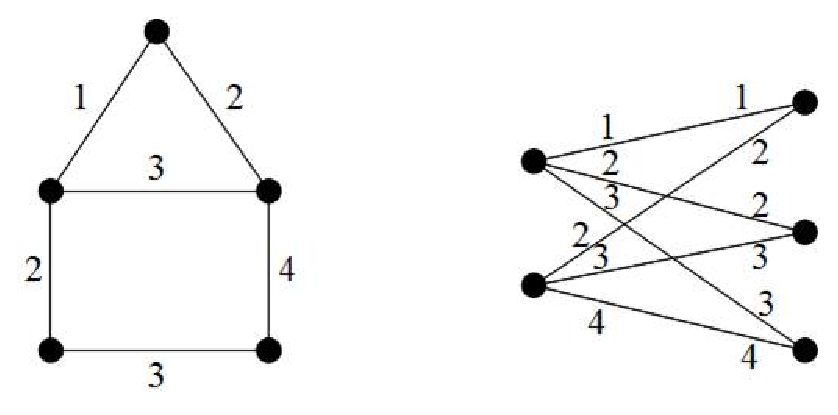
\includegraphics[width=20pc]{figures/W-bound-fig1.eps}\\
\caption{$3$ առավելագույն աստիճանով գրաֆներ, որոնք չունեն միջակայքային $3$-ներկում:}
\label{f1_cubic}
\end{center}
\end{figure}

Նկար \ref{f1_cubic}-ում պատկերված գրաֆները ցույց են տալիս, որ Թեորեմ \ref{t1_lower_matching_number}-ի ստորին գնահատականները հասանելի են: 

\begin{corollary}
\label{c1_lower_nopm} Եթե $G$ կապակցված մուլտիգրաֆը չունի կատարյալ զուգակցում և $G\in \mathfrak{N}$, ապա
\begin{center}
$w(G)\geq \max\{\Delta(G),2\delta(G)\}$:
\end{center}
\end{corollary}



Վերջապես, ապացուցենք Հետևանք \ref{c1_lower_nopm}-ի անալոգը կենտ մուլտիգրաֆների համար: $G$ մուլտիգրաֆը կանվանենք կենտ մուլտիգրաֆ, եթե $G$-ի բոլոր գագաթների աստիճանները կենտ են:

\begin{theorem}
\label{t1_lower_odd} Եթե $G$-ն կապակցված կենտ մուլտիգրաֆ է, $\vert
E(G)\vert-\frac{\vert V(G)\vert}{2}$ թիվը կենտ է և $G\in \mathfrak{N}$,
ապա
\begin{center}
$w(G)\geq \max\{\Delta(G),2\delta(G)\}$:
\end{center}
\end{theorem}
\begin{proof}[Ապացույց] Նշանակենք $\delta=\delta(G)$: Եթե $G$-ն չունի կատարյալ զուգակցում, ապա արդյունքը հետևում է Հետևանք \ref{c1_lower_nopm}-ից: Ենթադրենք $G$-ն ունի կատարյալ զուգակցում: Այժմ կատարենք հակասող ենթադրություն, դիցուք $G$-ն ունի $\alpha$ միջակայքային $t$-ներկում որևէ $t\leq 2\delta-1$ թվի համար: Քանի որ ցանկացած $v\in V(G)$, $1\leq \underline S\left(v,\alpha \right)\leq
\delta$, ստանում ենք, որ $\delta\in 
S_{\cap}\left(V(G),\alpha\right)$: Այստեղից հետևում է, որ $\delta$ գույնով ներկված կողերը $G$-ում կազմում են կատարյալ զուգակցում: Նշանակենք այդ կատարյալ զուգակցումը $M$-ով և դիտարկենք $G-M$ մուլտիգրաֆը: Սահմանենք $G-M$-ի $\beta$ ներկումը հետևյալ կերպ. ցանկացած $e\in E(G-M)$ կողի համար
\begin{center}
$\beta\left(e\right)=\left\{
\begin{tabular}{ll}
$\alpha(e)$, & երբ $1\leq \alpha(e)\leq \delta -1$,\\
$\alpha(e)-1$, & երբ $\delta+1\leq \alpha(e)\leq t$.\\
\end{tabular}%
\right.$
\end{center}

\begin{figure}[h]
\begin{center}
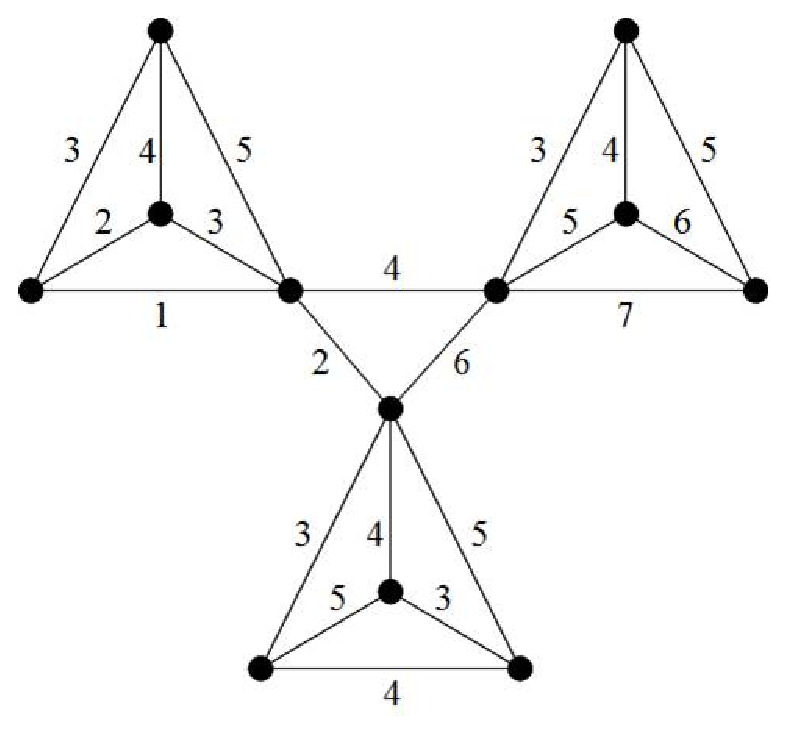
\includegraphics[width=20pc]{figures/W-bound-fig2.eps}\\
\caption{Միջակայքային ներկելի կապակցված գրաֆ $G$, որի բոլոր գագաթների աստիճանները կենտ են, $|E(G)|-\frac{|V(G)|}{2}=15$ և $w(G) \geq 6$:}
\label{f1_odd}
\end{center}
\end{figure}

Դժվար չէ տեսնել, որ $\beta$-ն $G-M$-ի միջակայքային $(t-1)$-ներկում է: Քանի որ $\vert E(G)\vert-\frac{\vert V(G)\vert}{2}$ կենտ է, ստանում ենք, որ $G-M$-ը զույգ մուլտիգրաֆ է կենտ թվով կողերով: Այստեղից հետևում է, որ $G-M$-ը ունի կենտ թվով կողեր պարունակող էյլերյան կապակցված բաղադրիչ, որը միջակայքային ներկելի է, ինչը հակասում է Հետևանք \ref{c1_eulerian}-ին:
\end{proof}

\begin{hide}
\subsection{Միջակայքային ներկման և հատուկ տիպի ֆակտորիզացիայի համարժեքությունը լրիվ գրաֆների համար}
\end{hide}
1.3 և 1.4 պարագրաֆները նվիրված են լրիվ գրաֆների միջակայքային ներկումների ուսումնասիրությանը: Հայտնի է, որ լրիվ գրաֆը ունի միջակայքային ներկում այն և միայն այն դեպքում, երբ գագաթների քանակը զույգ է: Հայտնի է նաև, որ $w(K_{2n})=2n-1$: Քամալյանը ստացել է $W(K_{2n}) \geq 2n-1 + \left\lfloor \log_2(2n-1) \right\rfloor$ գնահատականը, որը հետագայում լավացվել է Պետրոսյանի կողմից\footnote{P.A. Petrosyan, Interval edge-colorings of complete graphs and n-dimensional cubes, Discrete Math. 310, 2010, pp. 1580-1587.}.
\begin{hide}
\begin{theorem}\cite{Kamalian1990}
Ցանկացած $n\in \mathbb{N}$ թվի համար $W(K_{2n}) \geq 2n-1 + \left\lfloor \log_2(2n-1) \right\rfloor$:
\end{theorem}
\begin{theorem}\cite{Petrosyan2010}\label{tPetrosyan3n2}
Ցանկացած $n\in \mathbb{N}$ թվի համար $W(K_{2n}) \geq 3n-2$:
\end{theorem}
\begin{theorem}\cite{Petrosyan2010}\label{tPetrosyan4n}
Ցանկացած $n\in \mathbb{N}$ թվի համար $W(K_{4n}) \geq 4n-1 + W(K_{2n})$:
\end{theorem}
\end{hide}
\begin{theorem}
\label{t2_complete_pq} Եթե $n=p2^{q}$, որտեղ $p$-ն կենտ է, իսկ $q \in \mathbb{Z}_{\geq 0}$, ապա
\begin{center}
$W\left(K_{2n}\right)\geq 4n-2-p-q$:
\end{center}
\end{theorem}

\begin{hide}
\begin{hypothesis}
\label{h1_complete_pq}
Եթե $n=p2^{q}$, որտեղ $p$-ն կենտ է, իսկ $q \in \mathbb{Z}_+$, ապա
\begin{center}
$W\left(K_{2n}\right) = 4n-2-p-q$:
\end{center}
\end{hypothesis}
\end{hide}

\begin{hide}
\begin{figure}[b!]
\centering
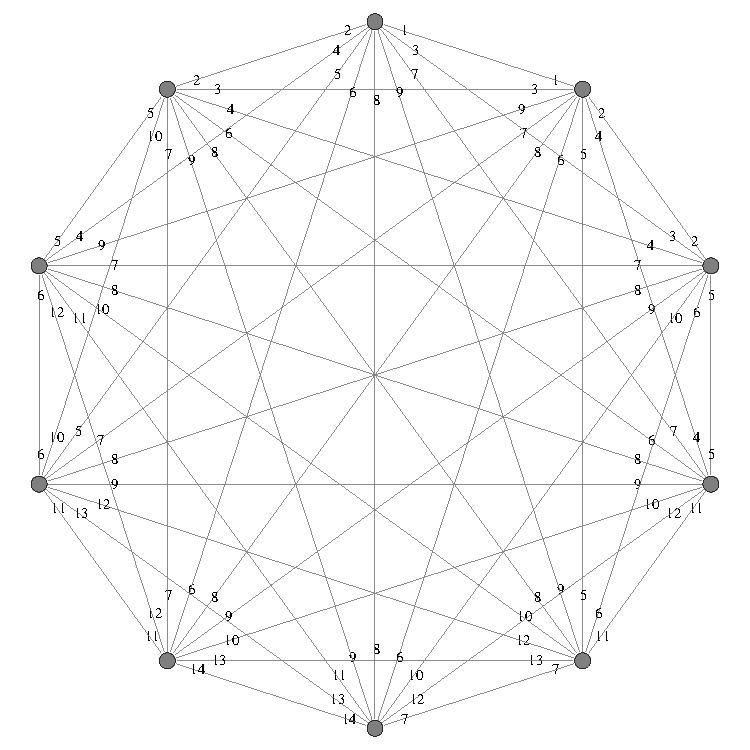
\includegraphics[width=0.74\textwidth]{figures/K_10-14.pdf}
\caption{$K_{10}$-ի միջակայքային $14$-ներկում: $sp(\alpha) = (1,2,1,1)$}
\label{t2_K10}
\end{figure}
\end{hide}

$W(K_{2n})$-ի հայտնի լավագույն վերին գնահատականը ստացել էին Գիառոն, Կուբալը և Մալաֆիյսկին. 
$W(K_{2n}) \leq 4n-4$, երբ $n \geq 2$:

\begin{hide}
\begin{hypothesis}
\label{h1_complete_log}
$W(K_{2n}) = 4n-2-\left \lfloor \log_2{n} \right \rfloor - \left \| n_2 \right \|$, որտեղ $\left \| n_2 \right \|$-ը $n$ թվի երկուական ներկայացման մեջ $1$-երի քանակն է:
\end{hypothesis}
\end{hide}
\begin{figure}[h]
\centering
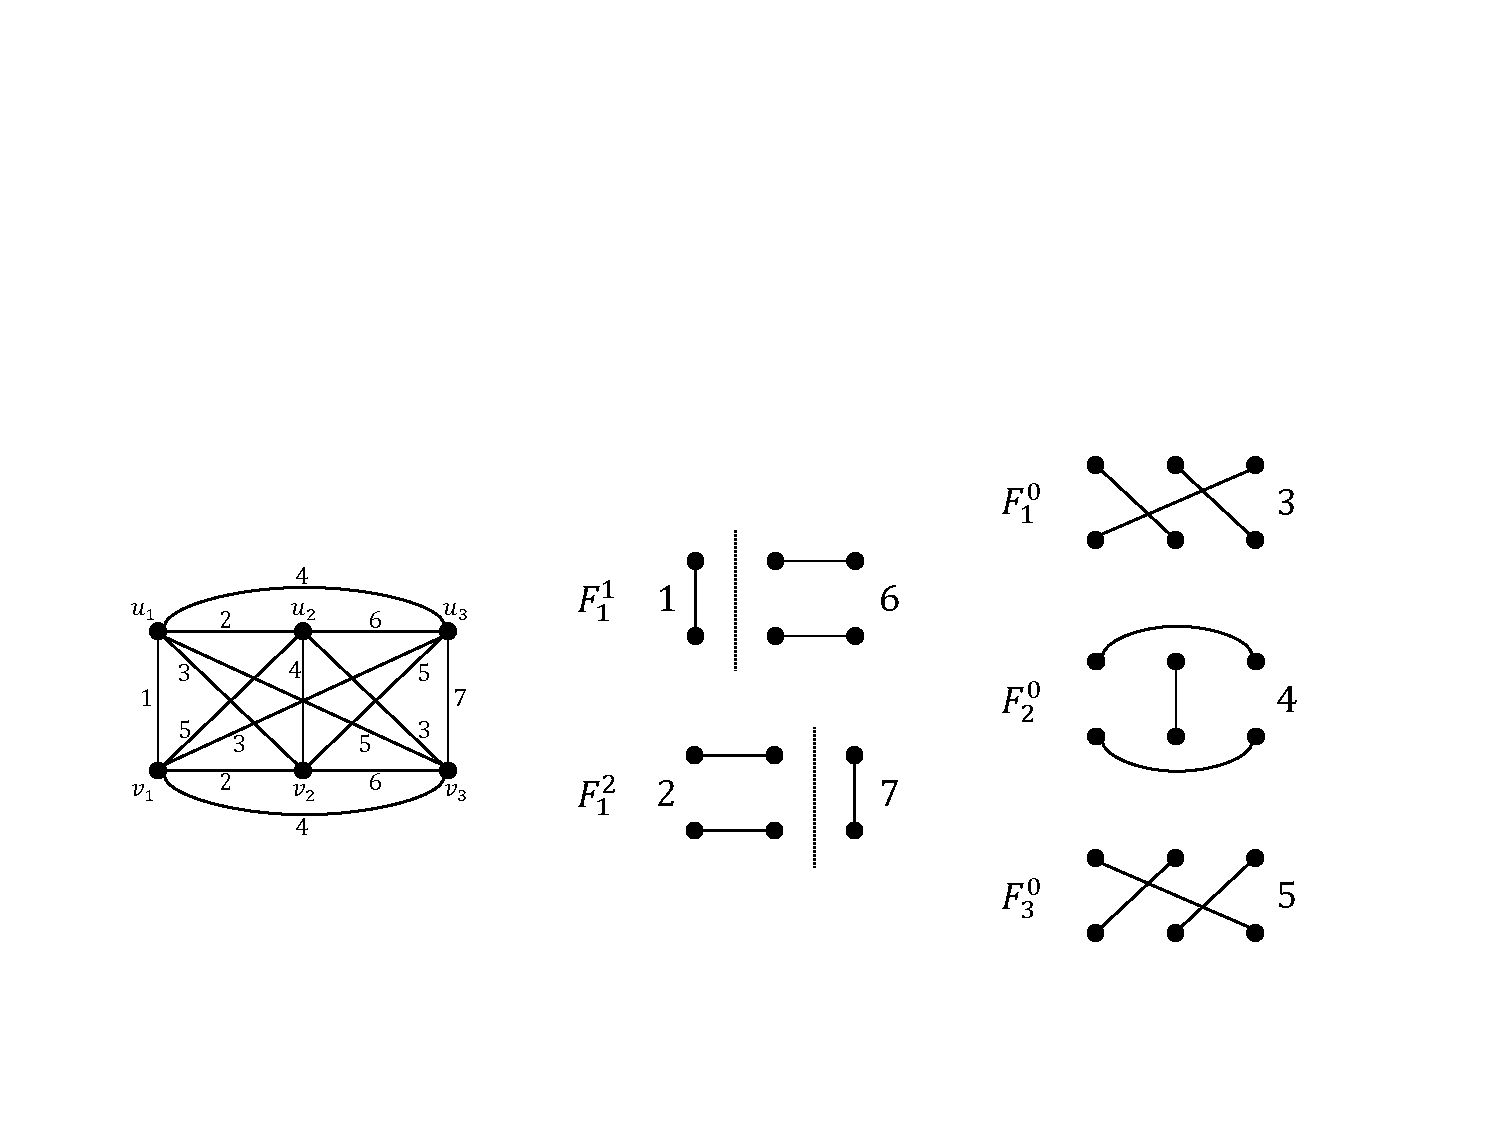
\includegraphics[width=0.7\textwidth]{figures/K_6factorization.pdf}
\caption{$K_6$-ի միջակայքային $7$-ներկումը և համապատասխան $1$-ֆակտորիզացիան՝ $\mathfrak{F}=\left\{F_1^1, F_1^2, F_1^0, F_2^0, F_3^0\right\}$}
\label{K_6factorization}
\end{figure}

$K_{2n}$ լրիվ գրաֆի գագաթների կամայական ֆիքսված $\mathbf{v} = \left(u_1,v_1, u_2,v_2, \ldots,u_n,v_n\right)$ համարակալման համար $H_{\mathbf{v}}^{[i,j]}$-ով, $i \leq j$, նշանակենք $K_{2n}$-ի $u_i, v_i, u_{i+1}, v_{i+1}, \ldots, u_j, v_j$ գագաթներով ծնված ենթագրաֆը: 

Դիցուք $\mathfrak{F} = \{F_1, F_2, \ldots, F_{2n-1}\}$ բազմությունը $K_{2n}$-ի $1$-ֆակտորիզացիա է: Ցանկացած $F\in \mathfrak{F}$ զուգակցման համար սահմանվում են իր \textit{ձախ և աջ մասերը} գագաթների $\mathbf{v}$ համարակալման նկատմամբ՝
\begin{center}
$l_{\mathbf{v}}^i(F) = F \cap E\left(H_{\mathbf{v}}^{[1,i]}\right)$ և
$r_{\mathbf{v}}^i(F) = F \cap E\left(H_{\mathbf{v}}^{[i+1,n]}\right)$:
\end{center}
Եթե որևէ $i$ թվի համար, $1 \leq i \leq n-1$, $F = l_{\mathbf{v}}^i(F) \cup r_{\mathbf{v}}^i(F)$, ապա $F$-ը կոչվում է \textit{$i$-բաժանված} կատարյալ զուգակցում $\mathbf{v}$ համարակալման նկատմամբ (օրինակ՝ $F_1^1$ և $F_1^2$ կատարյալ զուգակցումները Նկ. \ref{K_6factorization}-ում): Մի շարք լեմմաների օգնությամբ հաջողվել է ապացուցել լրիվ գրաֆի բաժանված կատարյալ զուգակցումներով ֆակտորիզացիաների և միջակայքային ներկումների համարժեքության լեմմա, որից բխում է հետևյալ արդյունքը.


\begin{hide}
\begin{remark}
\label{spectrumIntersection}
$K_{2n}$-ի ցանկացած $\alpha$ միջակայքային կողային ներկման համար, $S_\cap\left(K_{2n}, \alpha\right) \neq \emptyset$: Հակառակ դեպքում դա կհակասեր Թեորեմ \ref{t1_upper_2V-3}-ի վերին գնահատականին:
\end{remark}

\begin{lemma}
Եթե $1 \leq i \leq n$, ապա $\underline{S}(u_i, \alpha) = \underline{S}(v_i, \alpha)$.
\end{lemma}
\begin{proof}[Ապացույց]
Պնդում \ref{spectrumIntersection}-ից հետևում է, որ եթե $\underline{S}(v_i, \alpha) - \underline{S}(u_{i}, \alpha) > 0$, ապա $\underline{S}(u_{i}, \alpha)$ գույնով ներկված կողերը կազմում են կատարյալ զուգակցում $K_{2n}\left[\{u_1,v_1,u_2,v_2,\ldots,u_i\}\right]$ ենթագրաֆում, ինչը հնարավոր չէ, քանի որ այն ունի կենտ թվով գագաթներ:
\end{proof}

\begin{remark}
\label{totalShift}
Եթե $\alpha$-ն $K_{2n}$-ի միջակայքային $t$-ներկում է և ${\rm sh}(\alpha) = (b_1, b_2, \ldots, b_{n-1})$, ապա $t = 2n-1 + |{\rm sh}(\alpha)|$:
\end{remark}

\begin{remark}
\label{middleColors}
$K_{2n}$-ի կամայական $\alpha$ միջակայքային կողային ներկման համար բոլոր գագաթներում հանդիպող գույներն են. $S_\cap\left(K_{2n}, \alpha\right) = \left[\underline{S}(u_n, \alpha), \overline{S}(u_1, \alpha)\right] = \left[|{\rm sh}(\alpha)|+1, 2n-1\right] = \left\{|{\rm sh}(\alpha)|+j  : j=1,2,\ldots,2n-1-|{\rm sh}(\alpha)|\right\}$:
\end{remark}

\begin{remark}
\label{splittedColors}
Եթե $\alpha$-ն $K_{2n}$-ի միջակայքային $t$-ներկում է, և ${\rm sh}(\alpha) = (b_1, b_2, \ldots, b_{n-1})$, ապա
\begin{center}
\begin{tabular}{ll}
$L_{\mathbf{v}_\alpha}^i(\alpha) \subset S_\cap\left(H_{\mathbf{v}_\alpha}^{[1,i]},\alpha\right)$
&$L_{\mathbf{v}_\alpha}^i(\alpha) \cap S_\cup\left(H_{\mathbf{v}_\alpha}^{[i+1,n]},\alpha\right) = \emptyset$\\
$R_{\mathbf{v}_\alpha}^i(\alpha) \cap S_\cup\left(H_{\mathbf{v}_\alpha}^{[1,i]},\alpha\right) = \emptyset$ 
&$R_{\mathbf{v}_\alpha}^i(\alpha) \subset S_\cap\left(H_{\mathbf{v}_\alpha}^{[i+1,n]},\alpha\right)$
\end{tabular}
\end{center}
\end{remark}
\end{hide}

\begin{hide}
\begin{lemma}[Համարժեքության լեմմա]\label{lEquiv}
Հետևյալ երկու պնդումները համարժեք են.
\begin{description}
\item{(ա)} գոյություն ունի $K_{2n}$-ի $\alpha$ միջակայքային կողային ներկում այնպես, որ ${\rm sh}(\alpha) = (b_1, b_2, \ldots b_{n-1})$,
\item{(բ)} գոյություն ունի գագաթների $\mathbf{v}$ համարակալում և $K_{2n}$-ի $\mathfrak{F} = 
\left\{ F^0_j : j=1,2,\ldots,2n-1-\sum\limits_{i=1}^{n-1}b_i \right\}
\cup
\bigcup\limits_{i=1}^{n-1}\left\{F^i_j : j=1,2,\ldots,b_i\right\}$ $1$-ֆակտորիզացիա այնպես, որ $F^i_j$-ն $i$-բաժանված է $\mathbf{v}$ համարակալման նկատմամբ, $i=1,2,\ldots,n-1$, $j=1,2,\ldots,b_i$, $b_i \in \mathbb{Z}_+$:
\end{description}
\end{lemma}

\begin{proof}[Ապացույց]
Ապացույցի ընթացքում $B_i$-ով կնշանակենք $\sum\limits_{j=1}^{i}b_j$ գումարը, $i=0,1,\ldots,n-1$:

\begin{description}
\item{(ա) $=>$ (բ)}. Դիցուք $\alpha$-ն $K_{2n}$-ի միջակայքային $t$-ներկում է, որի համար ${\rm sh}(\alpha) = (b_1, b_2, \ldots b_{n-1})$: Ֆիքսենք գագաթների $\mathbf{v}_\alpha$ համարակալումը և կառուցենք $K_{2n}$-ի $\mathfrak{F}$ $1$-ֆակտորիզացիան: 

Պնդում \ref{middleColors}-ի համաձայն գոյություն ունեն $2n-1-|{\rm sh}(\alpha)|$ գույներ, որոնք հանդիպում են բոլոր գագաթների սպեկտրներում: Ըստ սահմանման, $|{\rm sh}(\alpha)| = \sum\limits_{i=1}^{n-1}b_i$, ուստի կարող ենք վերցնել $F_j^0 = C_{|{\rm sh}(\alpha)|+j}(\alpha)$, որտեղ $j=1,2,\ldots,2n-1-|{\rm sh}(\alpha)|$:

Պնդում \ref{splittedColors}-ից հետևում է, որ ցանկացած $i=1,2,\ldots,n-1$, թվի համար գոյություն ունեն $|L_{\mathbf{v}_\alpha}^i(\alpha)|=b_i$ իրարից տարբեր գույներ, որոնք հանդիպում են միայն գագաթների առաջին $i$ զույգերի սպեկտրներում, և ևս $|R_{\mathbf{v}_\alpha}^i(\alpha)|=b_i$ իրարից տարբեր գույներ, որոնք հանդիպում են միայն մնացած $2n-2i$ գագաթների սպեկտներում: Վերցնենք $F^i_j = C_{B_{i-1} + j}(\alpha) \cup C_{B_{i-1} + 2n - 1 + j}(\alpha)$, կամայական $i=1,2,\ldots,n-1$ և $j=1,2,\ldots,b_i$ թվերի համար: Նկատենք, որ $L_{\mathbf{v}_\alpha}^i(\alpha) \cup R_{\mathbf{v}_\alpha}^i(\alpha)$ բազմության գույներով ներկված կողերը չեն հատում $i$-րդ և $(i+1)$-րդ գագաթների զույգերի միջև անցնող ուղղահայաց ուղիղը ($F_1^1$ և $F_1^2$ Նկ. \ref{K_6factorization}-ում), ուստի $F^i_j$-ն բոլոր թույլատրելի $j$-երի համար $i$-բաժանված կատարյալ զուգակցում է գագաթների $\mathbf{v}_\alpha$ համարակալման նկատմամբ:

\item{(բ) $=>$ (ա)}. Ենթադրենք $\mathfrak{F} = 
\left\{ F^0_j : j=1,2,\ldots,2n-1-|{\rm sh}(\alpha)| \right\}
\cup
\bigcup\limits_{i=1}^{n-1}\left\{F^i_j : j=1,2,\ldots,b_i\right\}$ $K_{2n}$-ի $1$-ֆակտորիզացիա է, ընդ որում $F_j^i$-ն $i$-բաժանված կատարյալ զուգակցում է գագաթների $\mathbf{v}=\left(u_1,v_1, u_2,v_2, \ldots,u_n,v_n\right)$ համարակալման նկատմամբ, $i=1,2,\ldots,n-1$, $j=1,2,\ldots,b_i$: Կառուցենք $K_{2n}$-ի $\alpha$ միջակայքային կողային ներկումը հետևյալ կերպ.

\begin{tabular}{lll}
$\alpha(e)=B_{i-1} + j$ & երբ $e \in l_{\mathbf{v}}^i(F_j^i)$ & $i=1,2,\ldots,n-1$, $j=1,2,\ldots,b_i$ \\
$\alpha(e)=B_{n-1} + j$ & երբ $e \in F_j^0$ & $j=1,2,\ldots,2n-1-B_{n-1}$\\
$\alpha(e)=B_{i-1} + 2n - 1 + j$ & երբ $e \in r_{\mathbf{v}}^i(F_j^i)$ & $i=1,2,\ldots,n-1$, $j=1,2,\ldots,b_i$
\end{tabular}

Այն փաստից, որ $F^i_j$-ն գագաթների $\mathbf{v}$ համարակալման նկատմամբ $i$-բաժանված կատարյալ զուգակցում է, հետևում է, որ $K_{2n}$-ի կամայական կող ստացել է որևէ գույն: Իրոք, $u_i$ (նաև $v_i$) գագաթը ծածկված է բոլոր $F_j^0$ զուգակցումներով, $j=1,2,\ldots,2n-1-B_{n-1}$, $F_j^{i'}$, զուգակցումների ձախ մասերով, $i'=i,i+1,\ldots,n-1$, և $F_j^{i'}$ զուգակցումների աջ մասերով, $i'=1,2,\ldots,i-1$, կամայական $j=1,2,\ldots,b_{i'}$ թվի համար: Ուստի գագաթների սպեկտրները կլինեն.
\begin{align*}
S(u_i, \alpha) = S(v_i, \alpha) &= \bigcup\limits_{i'=i}^{n-1}\{B_{i'-1} + j  : j=1,2,\ldots,b_{i'}\} \\
& \cup
\{B_{n-1} + j : j=1,2,\ldots,2n-1-B_{n-1}\} \\
& \cup
\bigcup\limits_{i'=1}^{i-1}\{B_{i'-1} + 2n-1 + j  : j=1,2,\ldots,b_{i'}\}\\
&= [B_{i-1}+1, B_{n-1}] \cup [B_{n-1}+1, 2n-1] \cup [2n, B_{i-1}+2n-1]\\
&= [B_{i-1}+1, B_{i-1}+2n-1]
\end{align*}

Սա ցույց է տալիս, որ $\alpha$-ն $K_{2n}$-ի  միջակայքային $(B_{n-1} + 2n-1)$-ներկում է: Լեմմայի ապացույցն ավարտելու համար անհրաժեշտ է ստուգել կառուցված $\alpha$ ներկման շեղումների վեկտորը: Նկատենք, որ կամայական $i=1,2,\ldots,n-1$, թվի համար ունենք, որ $\underline{S}(u_{i+1}, \alpha) - \underline{S}(u_{i}, \alpha) = B_{i}-B_{i-1} = b_i$: Սա նշանակում է, որ գագաթների $\mathbf{v}_\alpha$ համարակալումը համընկնում է $\mathbf{v}$ համարակալման հետ և ${\rm sh}(\alpha) = (b_1, b_2, \ldots, b_{n-1})$:
\end{description}

\end{proof}

\begin{remark}\label{splittedSameColor}
Համարժեքության լեմմայի ապացույցի առաջին մասում կառուցված $F_j^0$ զուգակցումների մի մասը ևս կարող են լինել բաժանված կատարյալ զուգակցումներ, սակայն նրանց թե՛ աջ և թե՛ ձախ մասերը $\alpha$ ներկման մեջ ունեն նույն գույնը: Օրինակ, երբ $|{\rm sh}(\alpha)|=0$, $F^0_{\alpha(u_1v_1)} = C_{\alpha(u_1v_1)}(\alpha)$ զուգակցումը $1$-բաժանված կատարյալ զուգակցում է գագաթների $\mathbf{v}_\alpha$ համարակալման նկատմամբ:
\end{remark}
\end{hide}

\begin{corollary}\label{cEquiv}
Ցանկացած $n\in\mathbb{N}$-ի համար $K_{2n}$-ը ունի միջակայքային $t$-ներկում այն և միայն այն դեպքում, երբ այն ունի այնպիսի $1$-ֆակտորիզացիա, որտեղ առնվազն $t-2n+1$ կատարյալ զուգակցումներ բաժանված են:
\end{corollary}
\begin{proof}[Ապացույց]
Տրված միջակայքային $t$-ներկմանը համապատասխանող $1$-ֆակտորիզացիայի կառուցումը անմիջականորեն հետևում է Պնդում \ref{totalShift}-ից և Համարժեքության լեմմայից: Պնդում \ref{splittedSameColor}-ից հետևում է, որ ստացված $1$-ֆակտորիզացիայում բաժանված կատարյալ զուգակցումների թիվը կարող է մեծ լինել $t-2n+1$ թվից:

Եթե տրված է $K_{2n}$-ի $1$-ֆակտորիզացիա, որտեղ առնվազն $t-2n+1$ կատարյալ զուգակցումներ բաժանված են, կարող ենք դրանցից ընտրել որևէ $t-2n+1$-ը, ապա դրանցից յուրաքանչյուրի համար ընտրել որևէ $i$ թիվ, որի համար այն $i$-բաժանված է (միևնույն կատարյալ զուգակցումը կարող է միաժամանակ լինել և՛ $i$-բաժանված, և՛ $i'$-բաժանված տարբեր $i$ և $i'$ թվերի համար, ընտրությունը կրկին կամայական է) և կիրառել Համարժեքության լեմման: Այսպիսով, ստացված ներկումը կարող է միակը չլինել:
\end{proof}

Այս հետևանքի հիման վրա 1.4 ենթագլխում ապացուցվել են $W(K_{2n})$-ի մի շարք նոր ստորին և վերին գնահատականներ:

\begin{hide}
\subsection{Լրիվ գրաֆի միջակայքային ներկման առավելագույն գույների քանակի գնահատականներ}
\end{hide}
\begin{frame}{Լրիվ գրաֆների միջակայքային ներկումներ}{$W(K_{2n})$ պարամետրի ստորին գնահատականներ}



\begin{itemize}
\item Եթե $n\in \mathbb{N}$, ապա $W(K_{2n}) \geq 3n-2$ (Պետրոսյան, 2010)
\end{itemize}

\begin{theorem}[1.4.2]
Եթե $n \geq 2$, ապա $W(K_{2n}) \geq \lfloor 3.5n \rfloor - 3$:
\end{theorem}

\begin{figure}[b!]
\centering
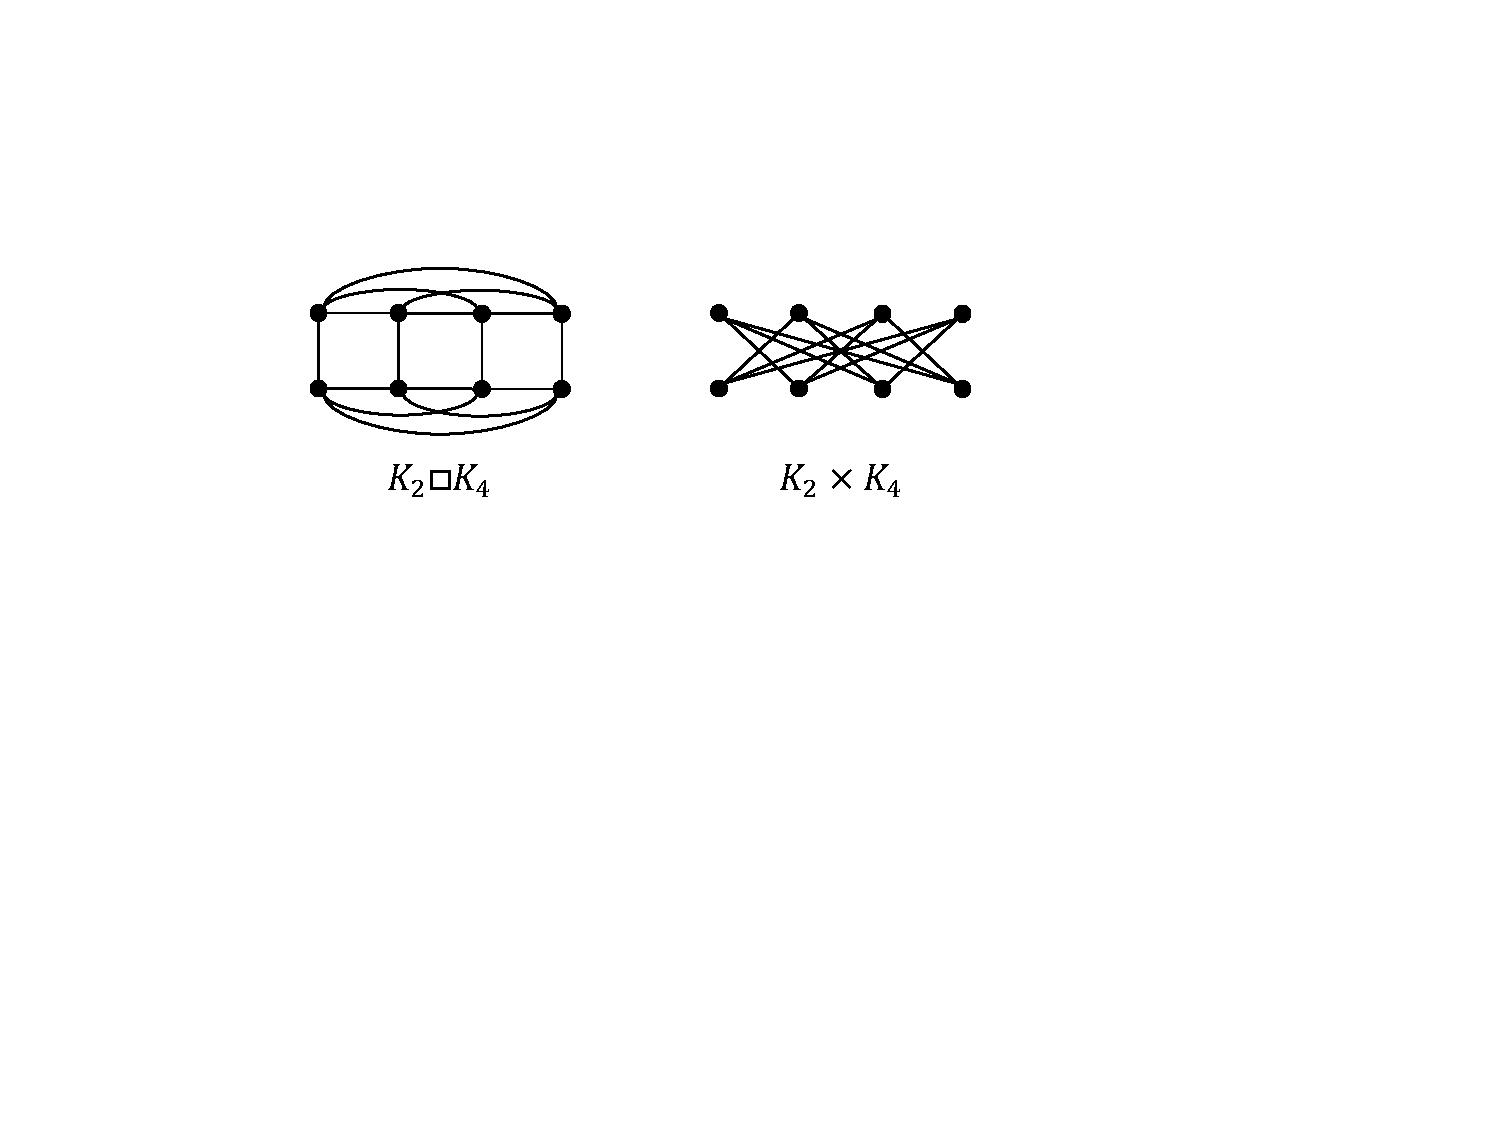
\includegraphics[width=0.8\textwidth]{figures/K_8products.pdf}
\label{K_8products}
\end{figure}

\end{frame}

\begin{frame}{Լրիվ գրաֆների միջակայքային ներկումներ}{$W(K_{2n})$ պարամետրի ստորին գնահատականներ}

\begin{itemize}
\item Ցանկացած $n\in \mathbb{N}$ թվի համար $W(K_{4n}) \geq W(K_{2n}) + 4n-1$ (Պետրոսյան, 2010)
\end{itemize}

\begin{theorem}[1.4.4]
Ցանկացած $m,n \in\mathbb{N}$ թվերի համար
\begin{center}
$W(K_{2mn}) \geq W(K_{2m}) + W(K_{2n}) + 4(m-1)(n-1) - 1$:
\end{center}
\end{theorem}

\begin{figure}[t!]
\centering
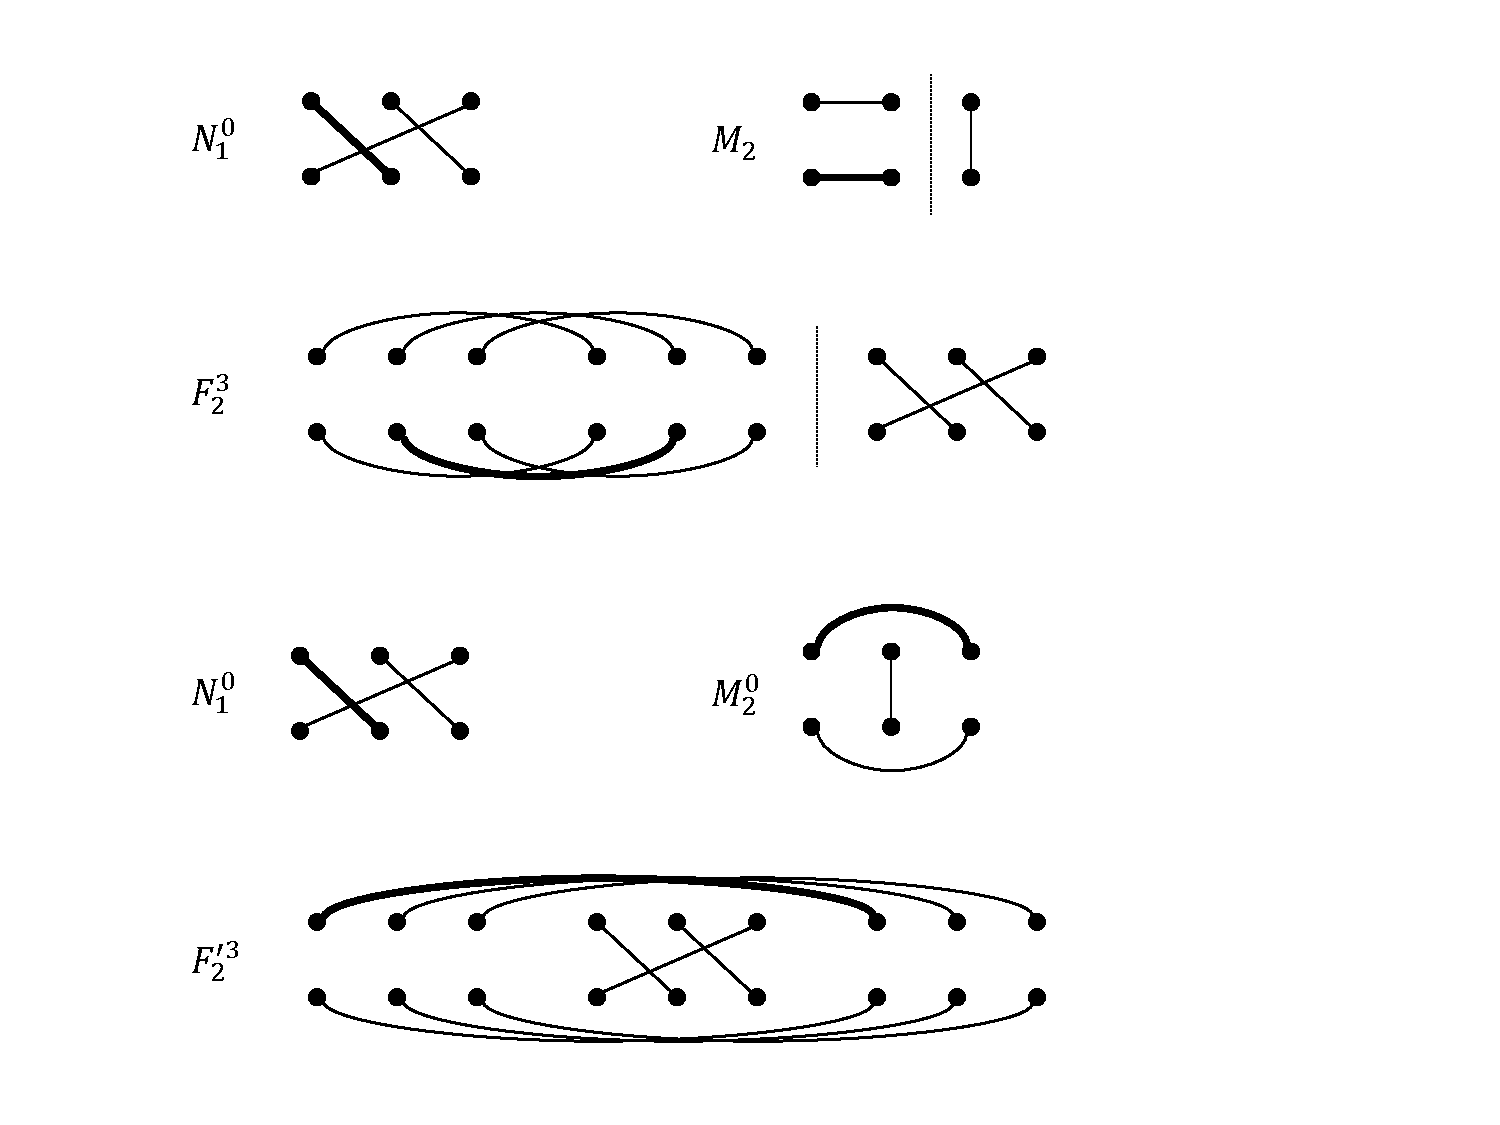
\includegraphics[trim={0 10cm 0 0cm},clip,width=0.4\textwidth]{figures/K_18-2.pdf}
\hspace{0.5cm}
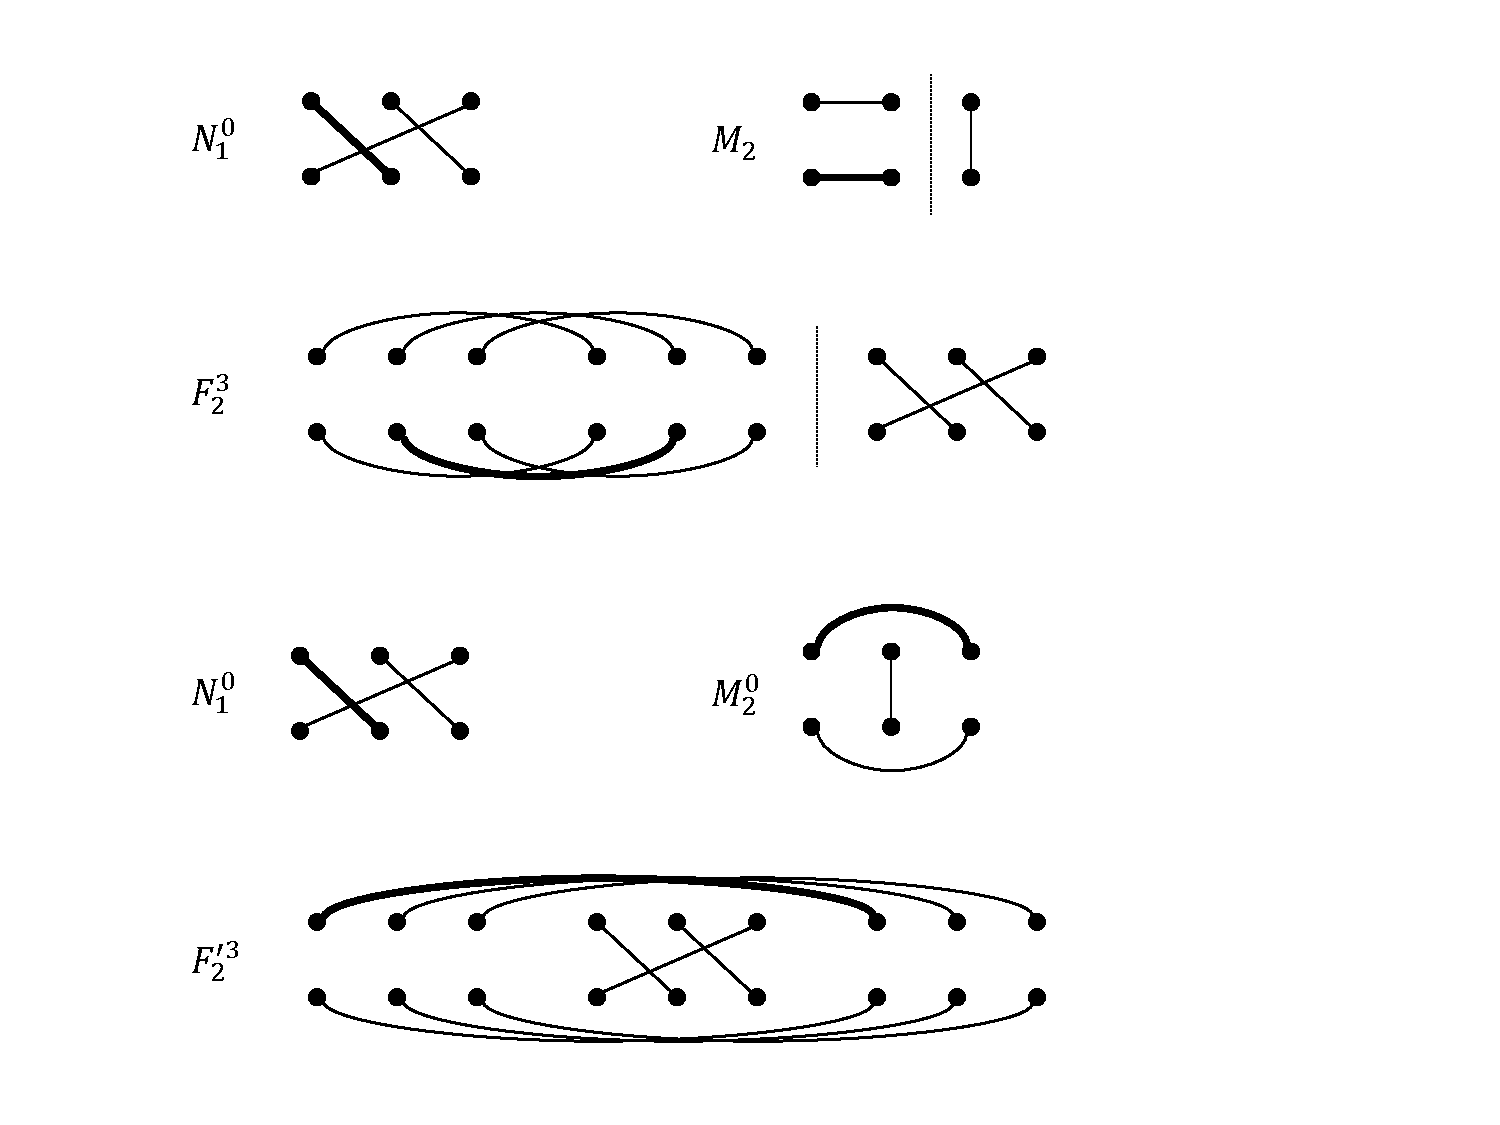
\includegraphics[trim={0 0.4cm 0 9cm},clip,width=0.4\textwidth]{figures/K_18-2.pdf}
\end{figure}

% Քանի որ $W(K_6) = 7$ և $W(K_{10}) \geq 14$, ուստի $W(K_{30}) \geq 52$, հետևաբար այս արդյունքը հերքում է Հիպոթեզ \ref{h1_complete_log}-ը, ըստ որի $W(K_{30})=51$: 

\end{frame}

\begin{frame}{Լրիվ գրաֆների միջակայքային ներկումներ}{$W(K_{2n})$ պարամետրի ստորին գնահատականներ}

\begin{theorem}[1.4.5]
Եթե $n = \prod\limits_{i=1}^{\pi(n)}{p_i^{\alpha_i}}$, որտեղ $p_i$-ն $i$-րդ պարզ թիվն է, $\pi(n)$-ը՝ $n$-ը չգերազանցող պարզ թվերի քանակը, իսկ $\alpha_i \in \mathbb{Z}_{\geq 0}$, ապա
\begin{center}
$W(K_{2n}) \geq 4n - 3 - \sum\limits_{i=1}^{\pi(n)}{\alpha_i\left(4p_i-3-W(K_{2p_i})\right)}$:
\end{center}
\end{theorem}

\end{frame}

\begin{frame}{Լրիվ գրաֆների միջակայքային ներկումներ}{$W(K_{2n})$ պարամետրի վերին գնահատական}

\begin{itemize}
\item Եթե $n \geq 2$, ապա 
\begin{center}
$W(K_{2n}) \leq 4n-4$
\end{center} (Գիառո, Կուբալ, Մալաֆիյսկի, 2001)
\end{itemize}

\begin{theorem}[1.4.17]
Եթե $n \geq 3$, ապա
\begin{center}
$W(K_{2n}) \leq \left\{
\begin{tabular}{ll}
$4n-5$, & երբ $n \geq 3$,\\
$4n-6$, & երբ $n \geq 5$,\\
$4n-7$, & երբ $n \geq 9$:\\
\end{tabular}
\right.$
\end{center}
\end{theorem}

% 1.4 պարագրաֆի վերջում որոշվել են նաև $W(K_{2n})$ պարամետրի ճշգրիտ արժեքները, երբ $n \leq 12$ և $n=16$ (Աղյուսակ \ref{tableAll}): Այս արդյունքների համադրմամբ ստացվել է հետևյալ ստորին գնահատականը.
\end{frame}

\begin{frame}{Լրիվ գրաֆների միջակայքային ներկումներ}{$W(K_{2n})$ պարամետրի ստորին գնահատականներ}

Եթե $n=p2^{q}$, որտեղ $p$-ն կենտ է, իսկ $q \in \mathbb{Z}_{\geq 0}$, ապա
\begin{center}
$W\left(K_{2n}\right)\geq 4n-2-p-q$
\end{center} 
(Պետրոսյան, 2010)

\begin{theorem}[1.4.20]
Եթե $n = \prod\limits_{i=1}^{\pi(n)}{p_i^{\alpha_i}}$, որտեղ $p_i$-ն $i$-րդ պարզ թիվն է, $\pi(n)$-ը՝ $n$-ը չգերազանցող պարզ թվերի քանակը, իսկ $\alpha_i \in \mathbb{Z}_{\geq 0}$, ապա 
\begin{center}
$W(K_{2n}) \geq 4n - 3 - A_n$,
\end{center}
որտեղ $A_n = \alpha_1 + 2\alpha_2 + 3\alpha_3 + 4\alpha_4 + 4\alpha_5 + \frac{1}{2}\sum\limits_{i=6}^{\pi(n)}{\alpha_i(p_i+1)}$:
\end{theorem}

\end{frame}


\begin{frame}{Լրիվ գրաֆների միջակայքային ներկումներ}{$W(K_{2n})$ պարամետրի ճշգրիտ արժեքներ}
Ճշգրիտ արժեքները հայտնի են, երբ $n \leq 12$ և $n=16$:

\fontsize{7pt}{14}\selectfont
\begin{table}[h]
\centering
\begin{tabularx}{0.96\textwidth}{r||*{18}{c<{\hspace{-4.5pt}}|}}
$n$ 
& $1$ & $2$ & $3$ & $4$ & $5$ & $6$ & $7$ & $8$ & $9$ & $10$ & $11$ & $12$ & $13$ & $14$ & $15$ & $16$  \\ \hline\hline
$W(K_{2n}) \geq $ 
& $1$ & $4$ & $7$ & $11$ & $14$ & $18$ & $21$ & $26$ & $29$ & $33$ & $37$ & $41$ & $42$ & $46$ & $52$ & $57$ \\ \hline
$W(K_{2n}) = $
& $1$ & $4$ & $7$ & $11$ & $14$ & $18$ & $21$ & $26$ & $29$ & $33$ & $37$ & $41$ &  &  &  & $57$  \\ \hline
$W(K_{2n}) \leq $
& $1$ & $4$ & $7$ & $11$ & $14$ & $18$ & $22$ & $26$ & $29$ & $33$ & $37$ & $41$ & $45$ & $49$ & $53$ & $57$ 
\end{tabularx}
\end{table}
% \pause

% \fontsize{11pt}{12}\selectfont
% 2016-ին Հուդակը, Կարդոշը, Մադարասը և Վրբյարովան դիտարկել են այս խնդիրը առանց ներկման ճշտության պայմանի: \\Նրանք ցույց են տվել, որ այդ դեպքում գագաթների թվից կախված գույների քանակը խիստ աճում է:
\end{frame}

\begin{hide}
\subsection{Լրիվ բազմակողմանի գրաֆների միջակայքային ներկումներ}
\end{hide}
\begin{hide}
\begin{theorem}[Քամալյան, 1989]
$K_{m,n}$ լրիվ երկկողմանի գրաֆը ունի միջակայքային $t$-ներկում այն և միայն դեպքում, երբ $m+n-(m,n) \leq t \leq m+n-1$:
\end{theorem}
\end{hide}

\begin{frame}{Լրիվ բազմակողմանի գրաֆների միջակայքային ներկումներ}

\begin{itemize}
\item $K_{1,1,n}\in \mathfrak{N}$ այն և միայն դեպքում, երբ $n$-ը զույգ է (Ֆենգ, Հուանգ, 2007)
\end{itemize}

\begin{theorem}[1.5.5]
$K_{1,m,n}\in\mathfrak{N}$ այն և միայն դեպքում, երբ $(m+1,n+1)=1$:

Ընդ որում, եթե $(m+1,n+1)=1$, ապա $W(K_{1,m,n}) \leq m+n+1$:
\end{theorem}

\begin{theorem}[1.5.9]
$w(K_{1,m,m+1}) = W(K_{1,m,m+1}) = 2m+1$:
\end{theorem}
\end{frame}

\begin{frame}{$K_{l,m,n}$-ի միջակայքային ներկումներ ($l > 1$)}

\begin{theorem}[1.5.10]
$K_{l,m,l+m}$ լրիվ երեք կողմանի գրաֆները միջակայքային ներկելի են:
\end{theorem}

\begin{theorem}[1.5.11]
$K_{2n, 2n+1, 2n+2}$ լրիվ երեք կողմանի գրաֆները միջակայքային ներկելի են և $w(K_{2n, 2n+1, 2n+2})=8n+2$:
\end{theorem}

\begin{theorem}[1.5.12]
Եթե $l$-ը, $m$-ը և $n$-ը կենտ են, ապա $K_{l,m,n} \notin \mathfrak{N}$:
\end{theorem}

\end{frame}

\begin{frame}{Լրիվ բազմակողմանի գրաֆների միջակայքային ներկումներ}

% \begin{theorem}[Պետրոսյան, 2012]
% Եթե $K_{n,\ldots,n}$ լրիվ հավասարակշռված $r$-կողմանի գրաֆ է, ապա
% $K_{n,\ldots,n} \in \mathfrak{N}$ այն և միայն այն դեպքում, երբ $nr$-ն զույգ է: Ավելին, երբ $nr$-ն զույգ է, ապա $w(K_{n,\ldots,n}) = n(r-1)$ և $W(K_{n,\ldots,n}) \geq \left(
% \frac{3}{2}r-1 \right)n-1$:
% \end{theorem}

\begin{theorem}[1.5.13]
Եթե $r,n\in \mathbb{N}$ և $nr$ արտադրյալը զույգ է, ապա
\begin{center}
$W\left(K_{\underbrace{\scriptstyle n,\ldots,n}_{r}}\right) \geq 
\left\{\begin{matrix}
 nW(K_r) + n -1 & \text{երբ }r\text{-ը զույգ է,} \\ 
 \frac{n}{2}W(K_{2r}) - 1 &  \text{երբ }n\text{-ը զույգ է:} 
\end{matrix}\right.$
\end{center}
\end{theorem}

\begin{hide}
\begin{corollary}
Եթե $k,n\in \mathbb{N}$, $k=\prod\limits_{i=1}^{\infty}{p_i^{\alpha_i}}$, որտեղ $p_i$-ն $i$-րդ պարզ թիվն է, իսկ $\alpha_i \in \mathbb{Z}_+$, իսկ $nk$ արտադրյալը զույգ է, ապա
\begin{center}
$W\left(K_{\underbrace{\scriptstyle n,\ldots,n}_{k}}\right) \geq 
\left\{\begin{matrix}
 2kn - n - nA_k - 1 & \text{երբ }k\text{-ն զույգ է,} \\ 
 2kn - n - \frac{n}{2}\left(A_k+1\right) - 1 &  \text{երբ }n\text{-ը զույգ է,} 
\end{matrix}\right.$
\end{center}
որտեղ $A_k = \alpha_1 + 2\alpha_2 + 3\alpha_3 + 4\alpha_4 + 4\alpha_5 + \frac{1}{2}\sum\limits_{i=6}^{\infty}{\alpha_i(p_i+1)}$:
\end{corollary}

\end{hide}
\end{frame}




\begin{hide}
\section{Գրաֆների դեկարտյան արտադրյալների միջակայքային ներկումներ}

\subsection{Գրաֆների դեկարտյան արտադրյալի միջակայքային ներկելիությունը}
\end{hide}
\begin{frame}{Գրաֆների դեկարտյան արտադրյալ}{Սահմանում}
$G$ և $H$ գրաֆների $G\square H$ դեկարտյան արտադրյալը.
\begin{align*}
V(G \square H) &= V(G) \times V(H) \\
E(G \square H) &= \{(u_1,v_1)(u_2,v_2) : &(u_1=u_2 \text{ և } v_1v_2 \in E(H)) \text{ կամ } &\\ 
& &(v_1=v_2 \text{ և } u_1u_2 \in E(G) \}&
\end{align*}
\begin{figure}[t!]
    \centering
    \begin{tikzpicture}[style=thick,scale=0.55, every node/.style={scale=0.55}]
        \coordinate (V11) at (0cm,2cm);
        \coordinate (V12) at (4cm,2cm);
        \coordinate (V13) at (6cm,2cm);
        \coordinate (V14) at (8cm,2cm);
        \coordinate (V15) at (10cm,2cm);
        \coordinate (V21) at (0cm,4cm);
        \coordinate (V22) at (4cm,4cm);
        \coordinate (V23) at (6cm,4cm);
        \coordinate (V24) at (8cm,4cm);
        \coordinate (V25) at (10cm,4cm);
        \coordinate (V31) at (0cm,6cm);
        \coordinate (V32) at (4cm,6cm);
        \coordinate (V33) at (6cm,6cm);
        \coordinate (V34) at (8cm,6cm);
        \coordinate (V35) at (10cm,6cm);
        \coordinate (V41) at (0cm,9cm);
        \coordinate (V42) at (4cm,9cm);
        \coordinate (V43) at (6cm,9cm);
        \coordinate (V44) at (8cm,9cm);
        \coordinate (V45) at (10cm,9cm);
        
        \draw<4-> (V12) -- (V13) -- (V14) -- (V15);
        \draw<4-> (V22) -- (V23) -- (V24) -- (V25);
        \draw<4-> (V32) -- (V33) -- (V34) -- (V35) ;
        \draw (V42) -- (V43) -- (V44) -- (V45) ;
        
        \draw (V11) -- (V21) -- (V31);
        \draw<3-> (V12) -- (V22) -- (V32);
        \draw<3-> (V13) -- (V23) -- (V33);
        \draw<3-> (V14) -- (V24) -- (V34);
        \draw<3-> (V15) -- (V25) -- (V35);
        
        \draw<4-> (V12) edge [bend left=20] (V15);
        \draw<4-> (V22) edge [bend left=20] (V25);
        \draw<4-> (V32) edge [bend left=20] (V35);
        \draw (V42) edge [bend left=20] (V45);
        
        \draw[fill=black] (V11) circle (2pt) ;
        \draw<2->[fill=black] (V12) circle (2pt) ;
        \draw<2->[fill=black] (V13) circle (2pt) ;
        \draw<2->[fill=black] (V14) circle (2pt) ;
        \draw<2->[fill=black] (V15) circle (2pt) ;
        \draw[fill=black] (V21) circle (2pt) ;
        \draw<2->[fill=black] (V22) circle (2pt) ;
        \draw<2->[fill=black] (V23) circle (2pt) ;
        \draw<2->[fill=black] (V24) circle (2pt) ;
        \draw<2->[fill=black] (V25) circle (2pt) ;
        \draw[fill=black] (V31) circle (2pt) ;
        \draw<2->[fill=black] (V32) circle (2pt) ;
        \draw<2->[fill=black] (V33) circle (2pt) ;
        \draw<2->[fill=black] (V34) circle (2pt) ;
        \draw<2->[fill=black] (V35) circle (2pt) ;
%         \draw[fill=black] (V41) circle (2pt) ;
        \draw[fill=black] (V42) circle (2pt) ;
        \draw[fill=black] (V43) circle (2pt) ;
        \draw[fill=black] (V44) circle (2pt) ;
        \draw[fill=black] (V45) circle (2pt) ;
    \end{tikzpicture}
    \end{figure}
    
\end{frame}



\begin{frame}{Գրաֆների դեկարտյան արտադրյալների միջակայքային ներկելիությունը}


Եթե $G,H\in \mathfrak{N}$, ապա $G\square H\in \mathfrak{N}$ (Գիառո, Կուբալ, 2004)

\begin{table}[h]
    \def\arraystretch{1.8}

    \centering
    \begin{tabular}{c|c|c}
         & $G \square H \in \mathfrak{N}$ & $G \square H \notin \mathfrak{N}$ \\
         \hline
        $G \in \mathfrak{N}$, $H \in \mathfrak{N}$ & $G=H=K_2$ & հնարավոր չէ \\
        $G \in \mathfrak{N}$, $H \notin \mathfrak{N}$ & $G=K_2$, $H=K_3$ & $G=$\begin{tikzpicture}[baseline=-0.5ex]
        \draw[fill=black] (0:0) circle(1pt);
        \draw[fill=black] (30:0.5cm) circle(1pt);
        \draw[fill=black] (-30:0.5cm) circle(1pt);
        \draw[fill=black] (150:0.5cm) circle(1pt);
        \draw[fill=black] (-150:0.5cm) circle(1pt);
        \draw (30:0.5cm) -- (0:0) -- (150:0.5cm) -- (-150:0.5cm) -- (0:0) -- (-30:0.5cm) -- cycle;
        \end{tikzpicture}, $H=K_3$ \\ 
        $G \notin \mathfrak{N}$, $H \notin \mathfrak{N}$ & $G=H=P_{10}$ & $G=H=K_3$ \\ 
        
    \end{tabular}
\end{table}
\end{frame}



\begin{hide}
\subsection{Համասեռ գրաֆների դեկարտյան արտադրյալներ}
\end{hide}
\begin{frame}{Համասեռ գրաֆների դեկարտյան արտադրյալներ}

(Գիառո, Կուբալ, 2004) Եթե $G,H\in \mathfrak{N}$, ապա 
\begin{center}
$w(G\square H)\leq w(G)+w(H)$
\end{center}
\begin{center}
$W(G\square H)\geq W(G)+W(H)$
\end{center}


\begin{theorem}[2.2.1]
Եթե $G,H\in \mathfrak{N}$, ընդ որում $H$-ը $r$-համասեռ է, ապա.
\begin{center}
$W(G\square H)\geq W(G)+W(H)+r$:
\end{center}
\end{theorem}
\end{frame}

\begin{frame}{Սեպարաբել միջակայքային ներկումներ}
\begin{columns}
\begin{column}{0.57\textwidth}
    Դիցուք $G$-ն կապակցված է:\\
    Ֆիքսված $x \in V(G)$ գագաթի համար՝\\
    \begin{center}
    $V(G) = \bigcup\limits_{i=0}^{\epsilon(x)}N_i(x)$, որտեղ
    \end{center}
    \begin{center}
    $N_i(x)=\left\{ v \in V(G) : d(v,x)=i \right\}$,
    \end{center}
    \begin{center}
    $i=0,\ldots,\epsilon(x)$: 
    \end{center}
\end{column}
\begin{column}{0.43\textwidth}
\begin{figure}[t]
\centering
\begin{tikzpicture}[style=thick]
    \coordinate (V0) at (2cm,1cm);
    \coordinate (V11) at (1cm,2cm);
    \coordinate (V12) at (1.5cm,2cm);
    \coordinate (V13) at (2.5cm,2cm);
    \coordinate (V14) at (3cm,2cm);
    \coordinate (V21) at (1cm,3cm);
    \coordinate (V22) at (1.5cm,3cm);
    \coordinate (V23) at (2.5cm,3cm);
    \coordinate (V24) at (3cm,3cm);
    \coordinate (V31) at (0.8cm,3.9cm);
    \coordinate (V32) at (1.2cm,3.9cm);
    \coordinate (V33) at (2.5cm,3.9cm);
    \coordinate (V34) at (2.8cm,3.9cm);
    \coordinate (V35) at (3.2cm,3.9cm);
    \coordinate (V41) at (0.8cm,4.6cm);
    \coordinate (V42) at (1.1cm,4.6cm);
    \coordinate (V43) at (1.5cm,4.6cm);
    \coordinate (V44) at (2.4cm,4.6cm);
    \coordinate (V45) at (3cm,4.6cm);
    \coordinate (Vn1) at (1cm,5.5cm);
    \coordinate (Vn2) at (1.5cm,5.5cm);
    \coordinate (Vn3) at (2.5cm,5.5cm);
    \coordinate (Vn4) at (3cm,5.5cm);
    
    \draw (V0) -- (V11);
    \draw (V0) -- (V12);
    \draw (V0) -- (V13);
    \draw (V0) -- (V14);
    \draw (V13) -- (V14);
    
    \draw (V11) -- (V21);
    \draw (V11) -- (V22);
    \draw (V12) -- (V22);
    \draw (V13) -- (V23);
    \draw (V13) -- (V24);
    
    \draw (V21) -- (V31);
    \draw (V21) -- (V32);
    \draw (V23) -- (V33);
    \draw (V24) -- (V34);
    \draw (V24) -- (V35);
    
    \draw (V41) -- (Vn1);
    \draw (V42) -- (Vn2);
    \draw (V43) -- (Vn2);
    \draw (V44) -- (Vn3);
    \draw (V45) -- (Vn4);
    \draw (Vn3) -- (Vn4);
    
    \draw[dotted,rounded corners=5pt]
  (0,1) node[left]{$N_0(x)$} ++(0,-0.25) rectangle ++(3.3,0.5) ;
  
  \draw[dotted,rounded corners=5pt]
  (0,2) node[left]{$N_1(x)$} ++(0,-0.25) rectangle ++(3.3,0.5) ;
  
  \draw[dotted,rounded corners=5pt]
  (0,3) node[left]{$N_2(x)$} ++(0,-0.25) rectangle ++(3.3,0.5) ;
  \draw[dotted,rounded corners=5pt]
  (0,5.5) node[left]{$N_{\epsilon(x)}(x)$} ++(0,-0.25) rectangle ++(3.3,0.5) ;
    
    \draw[fill=black] (V0) circle (2pt) node[right]{$x$};
    \draw[fill=black] (V11) circle (2pt);
    \draw[fill=black] (V12) circle (2pt);
    \draw[fill=black] (V13) circle (2pt);
    \draw[fill=black] (V14) circle (2pt);
    \draw[fill=black] (V21) circle (2pt);
    \draw[fill=black] (V22) circle (2pt);
    \draw[fill=black] (V23) circle (2pt);
    \draw[fill=black] (V24) circle (2pt);
    \draw[fill=black] (Vn1) circle (2pt);
    \draw[fill=black] (Vn2) circle (2pt);
    \draw[fill=black] (Vn3) circle (2pt);
    \draw[fill=black] (Vn4) circle (2pt);
\end{tikzpicture}
\end{figure}
\end{column}
\end{columns}
\end{frame}

\begin{frame}{Սեպարաբել միջակայքային ներկումներ}
\begin{figure}[b!]
\centering
\begin{tikzpicture}[style=thick,scale=0.8, every node/.style={scale=0.8}]
    \node at (-0.5cm, 1cm) {$N_{i-1}(x)$};
    \node at (-0.5cm, 2.5cm) {$N_i(x)$};
    \node at (-0.5cm, 4cm) {$N_{i+1}(x)$};
    
% first sample
    \coordinate (V111) at (1cm,1cm);
    \coordinate (V112) at (1.5cm,1cm);
    \coordinate (V113) at (2cm,1cm);
    \coordinate (V121) at (1cm,2.5cm);
    \coordinate (V122) at (1.5cm,2.5cm);
    \coordinate (V123) at (2cm,2.5cm);
    \coordinate (V131) at (1cm,4cm);
    \coordinate (V132) at (1.5cm,4cm);
    \coordinate (V133) at (2cm,4cm);
    
    \draw (V111) -- (V122);
    \draw (V112) -- (V122);
    \draw (V113) -- (V122);
    \draw (V121) -- (V122);
    \draw (V123) -- (V122);
    \draw (V131) -- (V122);
    \draw (V132) -- (V122);
    \draw (V133) -- (V122);
    
    \draw[fill=black] (V111) circle (2pt);
    \draw[fill=black] (V112) circle (2pt);
    \draw[fill=black] (V113) circle (2pt);
    \draw[fill=black] (V121) circle (2pt);
    \draw[fill=black] (V122) circle (2pt) node[right] at (1.55cm,2.7cm) {$v$};
    \draw[fill=black] (V123) circle (2pt);
    \draw[fill=black] (V131) circle (2pt);
    \draw[fill=black] (V132) circle (2pt);
    \draw[fill=black] (V133) circle (2pt);
    
    \node at (1.5cm, 0.3cm) {$S(v,\alpha)$};
    
% second sample
    \coordinate (V211) at (4cm,1cm);
    \coordinate (V212) at (4.5cm,1cm);
    \coordinate (V213) at (5cm,1cm);
    \coordinate (V221) at (4cm,2.5cm);
    \coordinate (V222) at (4.5cm,2.5cm);
    \coordinate (V223) at (5cm,2.5cm);
    \coordinate (V231) at (4cm,4cm);
    \coordinate (V232) at (4.5cm,4cm);
    \coordinate (V233) at (5cm,4cm);
    
    \draw (V211) -- (V222);
    \draw (V212) -- (V222);
    \draw (V213) -- (V222);
    \draw (V221) -- (V222);
    \draw (V223) -- (V222);
    \draw[dotted] (V231) -- (V222);
    \draw[dotted] (V232) -- (V222);
    \draw[dotted] (V233) -- (V222);
    
    \draw[fill=black] (V211) circle (2pt);
    \draw[fill=black] (V212) circle (2pt);
    \draw[fill=black] (V213) circle (2pt);
    \draw[fill=black] (V221) circle (2pt);
    \draw[fill=black] (V222) circle (2pt) node[right] at (4.55cm,2.7cm) {$v$};
    \draw[fill=black] (V223) circle (2pt);
    \draw[fill=black] (V231) circle (2pt);
    \draw[fill=black] (V232) circle (2pt);
    \draw[fill=black] (V233) circle (2pt);
    
    \node at (4.5cm, 0.3cm) {$S_x^{-}(v,\alpha)$};
    
% third sample
    \coordinate (V311) at (7cm,1cm);
    \coordinate (V312) at (7.5cm,1cm);
    \coordinate (V313) at (8cm,1cm);
    \coordinate (V321) at (7cm,2.5cm);
    \coordinate (V322) at (7.5cm,2.5cm);
    \coordinate (V323) at (8cm,2.5cm);
    \coordinate (V331) at (7cm,4cm);
    \coordinate (V332) at (7.5cm,4cm);
    \coordinate (V333) at (8cm,4cm);
    
    \draw[dotted] (V311) -- (V322);
    \draw[dotted] (V312) -- (V322);
    \draw[dotted] (V313) -- (V322);
    \draw[dotted] (V321) -- (V322);
    \draw[dotted] (V323) -- (V322);
    \draw (V331) -- (V322);
    \draw (V332) -- (V322);
    \draw (V333) -- (V322);
    
    \draw[fill=black] (V311) circle (2pt);
    \draw[fill=black] (V312) circle (2pt);
    \draw[fill=black] (V313) circle (2pt);
    \draw[fill=black] (V321) circle (2pt);
    \draw[fill=black] (V322) circle (2pt) node[right] at (7.55cm,2.7cm) {$v$};
    \draw[fill=black] (V323) circle (2pt);
    \draw[fill=black] (V331) circle (2pt);
    \draw[fill=black] (V332) circle (2pt);
    \draw[fill=black] (V333) circle (2pt);
    
    \node at (7.5cm, 0.3cm) {$S_x^{+}(v,\alpha)$};
    
\end{tikzpicture}
\label{vertexSpectrums}
\end{figure}
\fontsize{10pt}{11}\selectfont

Բոլոր $v \in N_i(G)$ գագաթների սպեկտրները տրոհենք 2 մասի.
\begin{align*}
S_x^-(v,\alpha) &= \left\{ \alpha(vu) : u\in N_{i-1}(x) \cup N_i(x) \right\}\\
S_x^+(v,\alpha) &= \left\{ \alpha(vu) : u\in N_{i+1}(x) \right\}
\end{align*}

Կասենք, որ $G$ կապակցված գրաֆի $\alpha$ միջակայքային ներկումը \textbf{սեպարաբել} է $x$ գագաթի նկատմամբ, եթե ցանկացած $\forall v \in V(G)$ գագաթի համար $\max S_x^-(v,\alpha) < \min S_x^+(v,\alpha)$:
\end{frame}

\begin{frame}{Սեպարաբել միջակայքային ներկումներ}
\begin{columns}
\begin{column}{0.5\textwidth}
   \begin{theorem}[2.2.4]
    Դիցուք $G$ կապակցված գրաֆը ունի սեպարաբել միջակայքային $t_G$-ներկում որևէ $x\in V(G)$ գագաթի նկատմամբ, ընդ որում գոյություն ունի $y\in N_{\epsilon(x)}(x)$ գագաթ, որի սպեկտրը պարունակում է $t_G$ գույնը, իսկ $1\in S(x,\alpha)$: Եթե $H$ գրաֆը $r$-համասեռ է և ունի միջակայքային $t_H$-ներկում, ապա
    \begin{center}
    $W(G \square H) \geq t_G + t_H + \epsilon(x)r$:
    \end{center}
    \end{theorem}

\end{column}
\begin{column}{0.5\textwidth}  %%<--- here
    \begin{figure}[t]
\centering
\begin{tikzpicture}[style=thick]
    \coordinate (V0) at (2cm,1cm);
    \coordinate (V11) at (1cm,2cm);
    \coordinate (V12) at (1.5cm,2cm);
    \coordinate (V13) at (2.5cm,2cm);
    \coordinate (V14) at (3cm,2cm);
    \coordinate (V21) at (1cm,3cm);
    \coordinate (V22) at (1.5cm,3cm);
    \coordinate (V23) at (2.5cm,3cm);
    \coordinate (V24) at (3cm,3cm);
    \coordinate (V31) at (0.8cm,3.9cm);
    \coordinate (V32) at (1.2cm,3.9cm);
    \coordinate (V33) at (2.5cm,3.9cm);
    \coordinate (V34) at (2.8cm,3.9cm);
    \coordinate (V35) at (3.2cm,3.9cm);
    \coordinate (V41) at (0.8cm,4.6cm);
    \coordinate (V42) at (1.1cm,4.6cm);
    \coordinate (V43) at (1.5cm,4.6cm);
    \coordinate (V44) at (2.4cm,4.6cm);
    \coordinate (V45) at (3cm,4.6cm);
    \coordinate (Vn1) at (1cm,5.5cm);
    \coordinate (Vn2) at (1.5cm,5.5cm);
    \coordinate (Vn3) at (2.5cm,5.5cm);
    \coordinate (Vn4) at (3cm,5.5cm);
    
    \draw (V0) -- node[left] {$1$} (V11);
    \draw (V0) -- (V12);
    \draw (V0) -- (V13);
    \draw (V0) -- (V14);
    \draw (V13) -- (V14);
    
    \draw (V11) -- (V21);
    \draw (V11) -- (V22);
    \draw (V12) -- (V22);
    \draw (V13) -- (V23);
    \draw (V13) -- (V24);
    
    \draw (V21) -- (V31);
    \draw (V21) -- (V32);
    \draw (V23) -- (V33);
    \draw (V24) -- (V34);
    \draw (V24) -- (V35);
    
    \draw (V41) -- (Vn1);
    \draw (V42) -- (Vn2);
    \draw (V43) -- (Vn2);
    \draw (V44) -- (Vn3);
    \draw (V45) -- node[right] {$t_G$} (Vn4);
    \draw (Vn3) -- (Vn4);
    
    \draw[dotted,rounded corners=5pt]
  (0,1) node[left]{$N_0(x)$} ++(0,-0.25) rectangle ++(3.3,0.5) ;
  
  \draw[dotted,rounded corners=5pt]
  (0,2) node[left]{$N_1(x)$} ++(0,-0.25) rectangle ++(3.3,0.5) ;
  
  \draw[dotted,rounded corners=5pt]
  (0,3) node[left]{$N_2(x)$} ++(0,-0.25) rectangle ++(3.3,0.5) ;
  \draw[dotted,rounded corners=5pt]
  (0,5.5) node[left]{$N_{\epsilon(x)}(x)$} ++(0,-0.25) rectangle ++(3.3,0.5) ;
    
    \draw[fill=black] (V0) circle (2pt) node[right]{$x$};
    \draw[fill=black] (V11) circle (2pt);
    \draw[fill=black] (V12) circle (2pt);
    \draw[fill=black] (V13) circle (2pt);
    \draw[fill=black] (V14) circle (2pt);
    \draw[fill=black] (V21) circle (2pt);
    \draw[fill=black] (V22) circle (2pt);
    \draw[fill=black] (V23) circle (2pt);
    \draw[fill=black] (V24) circle (2pt);
    \draw[fill=black] (Vn1) circle (2pt);
    \draw[fill=black] (Vn2) circle (2pt);
    \draw[fill=black] (Vn3) circle (2pt);
    \draw[fill=black] (Vn4) circle (2pt);
\end{tikzpicture}
\end{figure}

\end{column}
\end{columns}
\end{frame}

\begin{frame}{Սեպարաբել միջակայքային ներկումներ}

\begin{figure}[t!]
\centering
\begin{tikzpicture}[style=thick,scale=0.7, every node/.style={scale=0.7}]
% C_8
    \coordinate (c0) at (-0.5cm,1.5cm);
    \coordinate (c11) at (-1cm,3cm);
    \coordinate (c12) at (-1cm,4.5cm);
    \coordinate (c13) at (-1cm,6cm);
    \coordinate (c21) at (0cm,3cm);
    \coordinate (c22) at (0cm,4.5cm);
    \coordinate (c23) at (0cm,6cm);
    \coordinate (c4) at (-0.5cm,7.5cm);
    
    \draw (c0) -- node[left] {$1$} (c11) 
    -- node[left] {$2$} (c12) 
    -- node[left] {$3$} (c13) 
    -- node[left] {$4$} (c4);
    \draw (c0) -- node[right] {$2$} (c21) 
    -- node[right] {$3$} (c22) 
    -- node[right] {$4$} (c23) 
    -- node[right] {$5$} (c4);
    
    \draw[fill=black] (c0) circle (2pt)  node[right] {$x$};
    \draw[fill=black] (c11) circle (2pt) node[left] {$u_1$};
    \draw[fill=black] (c12) circle (2pt) node[left] {$u_2$};
    \draw[fill=black] (c13) circle (2pt) node[left] {$u_3$};
    \draw[fill=black] (c21) circle (2pt) node[right] {$v_1$};
    \draw[fill=black] (c22) circle (2pt) node[right] {$v_2$};
    \draw[fill=black] (c23) circle (2pt) node[right] {$v_3$};
    \draw[fill=black] (c4) circle (2pt) node[right] {$y$};
    
    \node at (-0.5cm, 0.3cm) {$C_8$};
    
% Caterpillar
    \coordinate (t0) at (2.5cm,1.5cm);
    \coordinate (t1) at (2.5cm,3cm);
    \coordinate (t21) at (2.5cm,4.5cm);
    \coordinate (t22) at (3.5cm,4.5cm);
    
    \coordinate (t31) at (2.5cm,6cm);
    \coordinate (t32) at (3.5cm,6cm);
    \coordinate (t33) at (4.5cm,6cm);
    
    \coordinate (t41) at (2.5cm,7.5cm);
    \coordinate (t42) at (3.5cm,7.5cm);
    \coordinate (t43) at (4.5cm,7.5cm);
    
    \coordinate (t5) at (2.5cm,9cm);
    
    \draw (t0) -- node[left] {$1$} (t1);
    \draw (t1) -- node[left] {$3$} (t21);
    \draw (t1) -- node[right] {$2$} (t22);
    \draw (t21) -- node[left] {$6$} (t31);
    \draw (t21) -- node[left] {$4$} (t32);
    \draw (t21) -- node[right] {$5$} (t33);
    \draw (t31) -- node[left] {$9$} (t41);
    \draw (t31) -- node[left] {$7$} (t42);
    \draw (t31) -- node[right] {$8$} (t43);
    \draw (t41) -- node[left] {$10$} (t5);
    
    \draw[fill=black] (t0) circle (2pt)  node[right] {$x=u_0$};
    \draw[fill=black] (t1) circle (2pt) node[left] {$u_1$};
    \draw[fill=black] (t21) circle (2pt) node[left] {$u_2$};
    \draw[fill=black] (t22) circle (2pt) node[right] {$v_2^1$};
    \draw[fill=black] (t31) circle (2pt) node[left] {$u_3$};
    \draw[fill=black] (t32) circle (2pt) node[right] {$v_3^1$};
    \draw[fill=black] (t33) circle (2pt) node[right] {$v_3^2$};
    \draw[fill=black] (t41) circle (2pt) node[left] {$u_4$};
    \draw[fill=black] (t42) circle (2pt) node[right] {$v_4^1$};
    \draw[fill=black] (t43) circle (2pt) node[right] {$v_4^2$};
    \draw[fill=black] (t5) circle (2pt)  node[right] {$y=u_5$};
    
    \node at (3cm, 0.3cm) {$T$};
    
    
% Q_3
    \coordinate (q000) at (7cm,1.5cm);
    \coordinate (q100) at (6cm,3cm);
    \coordinate (q010) at (7cm,3cm);
    \coordinate (q001) at (8cm,3cm);
    
    \coordinate (q110) at (6cm,4.5cm);
    \coordinate (q101) at (7cm,4.5cm);
    \coordinate (q011) at (8cm,4.5cm);
    \coordinate (q111) at (7cm,6cm);
    
    \draw (q000) -- node[left] {$1$} (q100);
    \draw (q000) -- node {$2$} (q010);
    \draw (q000) -- node[right] {$3$} (q001);
    
    \draw (q100) -- node[left] {$2$} (q110);
    \draw (q100) --  (q101);
    \draw (q010) -- node[right] {$3$} (q110);
    \draw (q010) --  (q011);
    \draw (q001) -- node[left] {$4$} (q101);
    \draw (q001) -- node[right] {$5$} (q011);
    
    \draw (q110) -- node[left] {$4$} (q111);
    \draw (q101) -- node {$5$} (q111);
    \draw (q011) -- node[right] {$6$} (q111);
    
    \draw[fill=black] (q000) circle (2pt)  node[right] {$x=(0,0,0)$};
    \draw[fill=black] (q100) circle (2pt);  
    \draw[fill=black] (q010) circle (2pt);  
    \draw[fill=black] (q001) circle (2pt);  
    \draw[fill=black] (q110) circle (2pt);  
    \draw[fill=black] (q101) circle (2pt);  
    \draw[fill=black] (q011) circle (2pt);  
    \draw[fill=black] (q111) circle (2pt) node[right] {$y=(1,1,1)$};  
    
    \node at (7cm, 0.3cm) {$Q_3$};
    
    
% K_3,3
    \coordinate (b0) at (11cm,1.5cm);
    \coordinate (b11) at (10cm,3cm);
    \coordinate (b12) at (11cm,3cm);
    \coordinate (b13) at (12cm,3cm);
    
    \coordinate (b21) at (10.5cm,4.5cm);
    \coordinate (b22) at (11.5cm,4.5cm);
    
    \draw (b0) -- node[left] {$1$} (b11);
    \draw (b0) -- node {$2$} (b12);
    \draw (b0) -- node[right] {$3$} (b13);
    
    \draw (b11) -- node[left] {$2$} (b21);
    \draw (b11) -- node[left] {$3$} (b22);
    \draw (b12) --  (b21);
    \draw (b12) --  (b22);
    \draw (b13) -- node[right] {$4$} (b21);
    \draw (b13) -- node[right] {$5$} (b22);
    
    \draw[fill=black] (b0) circle (2pt)  node[right] {$x=u_1$};
    \draw[fill=black] (b11) circle (2pt)  node[left] {$v_1$};  
    \draw[fill=black] (b12) circle (2pt)  node[right] {$v_2$};  
    \draw[fill=black] (b13) circle (2pt)  node[right] {$v_3$};  
    \draw[fill=black] (b21) circle (2pt)  node[left] {$u_2$};  
    \draw[fill=black] (b22) circle (2pt)  node[right] {$y=u_3$};  
    
    \node at (11cm, 0.3cm) {$K_{3,3}$};
    
    
\end{tikzpicture}
\end{figure}
\end{frame}

\begin{frame}[shrink]{Սեպարաբել միջակայքային ներկումներ}

\begin{corollary}[2.2.5]
Եթե $G$-ն հանդիսանում է 
\begin{itemize}
\item զույգ երկարությամբ ցիկլ,
\item շղթա,
\item n-չափանի խորանարդ,
\item թրթուրածառ կամ
\item լրիվ երկկողմանի գրաֆ,
\end{itemize}
իսկ $H$-ը միջակայքային ներկելի $r$-համասեռ գրաֆ է, ապա
\begin{center}
$W(G \square H) \geq W(G) + W(H) + \mathrm{diam}(G)r$:
\end{center}
\end{corollary}

\end{frame}

\begin{hide}
\subsection{Երկկողմանի գրաֆների դեկարտյան արտադրյալներ}
\end{hide}
Այս պարագրաֆում կդիտարկենք այնպիսի դեկարտյան արտադրյալներ, որոնց արտադրիչներից մեկը երկկողմանի գրաֆ է: Հայտնի է, որ երկկողմանի գրաֆների միջակայքային ներկելիությունը պարզելը NP-լրիվ խնդիր է \cite{Sevastyanov1990}: Մինչ այժմ բաց է մնում 4 առավելագույն աստիճան ունեցող երկկողմանի գրաֆների միջակայքային ներկելիության հարցը \cite{JensenToft1995,Stiebitz2012}: Այս պարագրաֆում ցույց կտանք, որ փոքր առավելագույն աստիճանով երկկողմանի գրաֆների որոշ դասերի դեկարտյան արտադրյալները $K_2$ գրաֆի հետ ունեն միջակայքային ներկումներ:

Նախ ցույց տանք, որ $h$-չափանի խորանարդի մասնակցությամբ դեկարտյան արտադրյալների ներկումները կապված են գրաֆների միջակայքային $(t,h)$-ներկումների հետ:

\begin{theorem}
\label{t2_cartesian_gap} $G\in \mathfrak{N}^{h}$ այն և միայն այն դեպքում, երբ $G\square
Q_{h}\in \mathfrak{N}$:
\end{theorem}
\begin{proof}[Ապացույց]
Դիցուք $\alpha$-ն $G$-ի միջակայքային $(t,h)$-ներկում է: Կառուցենք $G\square Q_{h}$ գրաֆի $\beta$ ներկումը հետևյալ կերպ: Նախ $G\square Q_{h}$-ի յուրաքանչյուր $G$-շերտ ներկենք $\alpha$ ներկման համաձայն: Այնուհետև, կամայական $u\in V(G)$ գագաթի համար, ներկենք $G\square Q_{h}$-ի համապատասխան $Q_{h}$-շերտը օգտագործելով $\overline
{S\left(u,\alpha \right)}$ բազմությունից $h$ գույներ: Պարզ է, որ ցանկացած $(u,v)\in V(G\square
Q_{h})$ գագաթի համար, $S\left((u,v),\beta \right)=S\left(u,\alpha \right)\cup
\overline{S\left(u,\alpha \right)}=\left[\underline S\left(u,\alpha
\right),\underline S\left(u,\alpha \right)+d_{G}(u)+h-1\right]$:
Այստեղից հետևում է $G\square Q_{h}\in \mathfrak{N}$:

Դիցուք $\gamma$-ն $G\square
Q_{h}$-ի միջակայքային $t^{\prime}$-ներկում է: Այս կողային ներկման սահմանափակումը $G\square Q_{h}$-ի որևէ $G$-շերտի կողերի վրա կարող է ձևափոխվել $G$-ի
միջակայքային $(t^{\prime\prime},h)$-ներկման, որտեղ $t^{\prime\prime}\leq
t^{\prime}$:
\end{proof} % բացել ապացույցը

Այս թեորեմից հետևում է, որ $G$ գրաֆի միջակայքային $h$-անցք-ներկելիության վերաբերյալ կամայական արդյունք կարելի է վերածել $G\square Q_{h}$ գրաֆի միջակայքային ներկելիության մասին արդյունքի: Ավելին, եթե $G$-ն երկկողմանի է, ապա $G\square Q_{h}$-ը ևս երկկողմանի է:

Այժմ դիտարկենք 4 առավելագույն աստիճան ունեցող երկկողմանի գրաֆների դեկարտյան արտադրյալները:

\begin{theorem}
\label{t2_bipartite_Delta4} Եթե $G$-ն երկկողմանի գրաֆ է, որի համար $\Delta(G)=4$,
ապա $G\in \mathfrak{N}^{1}$ և $w^{1}(G)=4$:
\end{theorem}
\begin{proof}[Ապացույց] Դիցուք $G$-ն երկկողմանի գրաֆ է 4 առավելագույն աստիճանով:
Հայտնի է, որ եթե $G$-ն չունի 3 աստիճանով գագաթ, ապա այն ունի միջակայքային $4$-ներկում \cite{Giaro1997}: Ուստի, $G\in
\mathfrak{N}^{1}$ և $w^{1}(G)=4$: Այժմ ենթադրենք, որ $G$-ն ունի 3 աստիճանով որոշ գագաթներ: Կառուցենք նոր $G^{\star}$ գրաֆը հետևյալ կերպ. $G$-ի յուրաքանչյուր $3$ աստիճան ունեցող գագաթին ավելացնենք կախված կող: Հեշտ է տեսնել, որ $G^{\star}$-ը երկկողմանի գրաֆ է 4 առավելագույն աստիճանով և չունի 3 աստիճանով գագաթներ, ուստի, այն ևս ունի միջակայքային $4$-ներկում: Այժմ դիտարկենք այս միջակայքային $4$-ներկման սահմանափակումը $G$-ի կողերի վրա: Պարզ է, որ այս ներկումը $G$-ի միջակայքային $(4,1)$-ներկում է:
\end{proof}

Թեորեմներ \ref{t2_cartesian_gap}-ի և \ref{t2_bipartite_Delta4}-ի համաձայն ստանում ենք հետևյալ արդյունքը.

\begin{corollary}
\label{c2_bipartite_Delta4} Եթե $G$-ն երկկողմանի գրաֆ է, որի համար $\Delta(G)\leq
4$, ապա $G\square K_{2}\in \mathfrak{N}$:
\end{corollary}

\cite{CarlJToft}-ում հեղինակները ցույց են տվել, որ բոլոր $(5,3)$-երկհամասեռ երկկողմանի գրաֆները միջակայքային $1$-անցք-ներկելի են: Այժմ դիտարկենք բոլոր երկկողմանի գրաֆները, որոնց առավելագույն աստիճանը 5 է:

\begin{theorem}
\label{t2_bipartite_Delta5_no3} Եթե $G$-ն երկկողմանի գրաֆ է, որի համար $\Delta(G)=5$ և չունի $3$ աստիճան ունեցող գագաթ, ապա $G\in \mathfrak{N}^{1}$ և
$w^{1}(G)=5$:
\end{theorem}
\begin{proof}[Ապացույց]
Դիցուք $G$-ն երկկողմանի գրաֆ է, որի առավելագույն աստիճանը $5$ է,
բայց չունի $3$ աստիճան ունեցող գագաթ: Ըստ Հոլլի թեորեմի, $G$-ն ունի առավելագույն աստիճան ունեցող գագաթները ծածկող զուգակցում: Դիցուք $M$-ը $G$-ի այդպիսի զուգակցում է: Դիտարկենք $G^{\prime}=G-M$ գրաֆը:
Պարզ է, որ $G^{\prime}$-ը երկկողմանի գրաֆ է, որի համար
$\Delta(G^{\prime})=4$: Ինչպես Թեորեմ \ref{t2_bipartite_Delta4}-ի ապացույցում, կարող ենք ցույց տալ, որ $G^{\prime}$-ը ունի $\alpha$ միջակայքային $(4,1)$-ներկում այնպիսին, որ կամայական $v\in
V(G^{\prime})$ գագաթի համար, որի համար $d_{G^{\prime}}(v)\in \{1,2,4\}$, $S(v,\alpha)$-ն ամբողջ թվերի միջակայք է: Այժմ կառուցենք $G^{\prime}$-ի նոր $\beta$ ներկումը վերցնելով $\alpha$ ներկման գույները և փոխարինելով 3 և 4 գույները համապատասխանաբար 4-ով և 5-ով: Այսպիսով, ամեն $v\in
V(G^{\prime})$ գագաթի համար կունենանք, որ

$\bullet$ եթե $d_{G^{\prime}}(v)=4$, ապա $S(v,\beta)=
\{1,2,4,5\}$,

$\bullet$ եթե $d_{G^{\prime}}(v)=3$, ապա
$S(v,\beta)\in \{\{1,2,4\},\{1,2,5\},\{1,4,5\},\{2,4,5\}\}$,

$\bullet$ եթե $d_{G^{\prime}}(v)=2$, ապա $S(v,\beta)\in
\{\{1,2\},\{2,4\},\{4,5\}\}$,

$\bullet$ եթե $d_{G^{\prime}}(v)=1$, ապա $S(v,\beta)\in
\{\{1\},\{2\},\{4\},\{5\}\}$:

Այժմ սահմանենք $G$-ի $\gamma$ կողային ներկումը հետևյալ կերպ.

1) կամայական $e\in E(G^{\prime})$ կողի համար $\gamma(e)=\beta(e)$,

2) կամայական $e\in M$ կողի համար $\gamma(e)=3$:

Քանի որ $G$-ն չունի $3$ աստիճան ունեցող գագաթ, ապա կամայական $v\in V(G)$ գագաթի համար ստանում ենք, որ

$\bullet$ եթե $d_{G}(v)=5$, ապա $S(v,\gamma)=[1,5]$,

$\bullet$ եթե $d_{G}(v)=4$, ապա $S(v,\gamma)\in
\{[1,4],[2,5],\{1,2,3,5\},\{1,2,4,5\},\{1,3,4,5\}\}$,

$\bullet$ եթե $d_{G}(v)=2$, ապա
$S(v,\gamma)\in
\{\{1,2\},\{2,4\},\{4,5\},\{1,3\},\{2,3\},\{3,4\},\{3,5\}\}$,

$\bullet$ եթե $d_{G}(v)=1$, ապա $S(v,\gamma)\in
\{\{1\},\{2\},\{3\},\{4\},\{5\}\}$:

Այստեղից հետևում է, որ $\gamma$-ն $G$-ի միջակայքային $(5,1)$-ներկում է:
\end{proof}

\begin{corollary}
\label{c2_bipartite_Delta5_no3} Եթե $G$-ն երկկողմանի գրաֆ է, որի համար $\Delta(G) =
5$, և չունի $3$ աստիճան ունեցող գագաթ, ապա $G\square K_{2}\in \mathfrak{N}$:
\end{corollary}

Նախորդ թեորեմում երեք աստիճան ունեցող գագաթների գոյություն չունենալու պայմանը կարող ենք փոխարինել կատարյալ զուգակցման գոյության պայմանով:

\begin{theorem}
\label{t2_bipartite_Delta5_nopm} Եթե $G$-ն կատարյալ զուգակցում ունեցող երկկողմանի գրաֆ է, որի համար $\Delta(G)=5$, ապա $G\in \mathfrak{N}^{1}$ և
$w^{1}(G)=5$:
\end{theorem}
\begin{proof}[Ապացույց]
Դիտարկենք $G' = G - M$ գրաֆը, որտեղ $M$-ը $G$-ում առկա որևէ կատարյալ զուգակցում է: Թեորեմ \ref{t2_bipartite_Delta5_no3}-ի ապացույցում նկարագրված եղանակով կարելի է կառուցել $G'$-ի $\beta$ ճիշտ կողային ներկում $1,2,4,5$ գույներով այնպես, որ ցանկացած $v\in
V(G^{\prime})$ գագաթի համար կունենանք հետևյալը.

$\bullet$ եթե $d_{G^{\prime}}(v)=4$, ապա $S(v,\beta)=
\{1,2,4,5\}$,

$\bullet$ եթե $d_{G^{\prime}}(v)=3$, ապա
$S(v,\beta)\in \{\{1,2,4\},\{1,2,5\},\{1,4,5\},\{2,4,5\}\}$,

$\bullet$ եթե $d_{G^{\prime}}(v)=2$, ապա $S(v,\beta)\in
\{\{1,2\},\{2,4\},\{4,5\}\}$,

$\bullet$ եթե $d_{G^{\prime}}(v)=1$, ապա $S(v,\beta)\in
\{\{1\},\{2\},\{4\},\{5\}\}$:

$G$ գրաֆի $\gamma$ ներկումը կստացվի $\beta$ ներկումից՝ $M$ կատարյալ զուգակցման կողերը $3$ գույնով ներկելով: Քանի որ $M$-ը ծածկում էր $G$-ի բոլոր գագաթները, $\gamma$ ներկման դեպքում գագաթների սպեկտրները կբավարարեն հետևյալ պայմաններին.

$\bullet$ եթե $d_{G^{\prime}}(v)=5$, ապա $S(v,\beta)=
[1,5]$,

$\bullet$ եթե $d_{G^{\prime}}(v)=4$, ապա
$S(v,\beta)\in \{[1,4],\{1,2,3,5\},\{1,3,4,5\},[2,5]\}$,

$\bullet$ եթե $d_{G^{\prime}}(v)=3$, ապա $S(v,\beta)\in
\{[1,3],[2,4],[3,5]\}$,

$\bullet$ եթե $d_{G^{\prime}}(v)=2$, ապա $S(v,\beta)\in
\{\{1,3\},\{2,3\},\{3,4\},\{3,5\}\}$,

$\bullet$ եթե $d_{G^{\prime}}(v)=1$, ապա $S(v,\beta) = \{3\}$:

Այսպիսով, $\gamma$-ն $G$-ի միջակայքային $(5,1)$-ներկում է և $w^1(G)=5$:
\end{proof}

\begin{corollary}
\label{c2_bipartite_Delta5_nopm} Եթե $G$-ն կատարյալ զուգակցում ունեցող երկկողմանի գրաֆ է, որի համար $\Delta(G)=5$, ապա $G \square K_2 \in \mathfrak{N}$:
\end{corollary}

\cite{CarlJToft}-ում հեղինակները ցույց են տվել, որ բոլոր $(6,4)$-երկհամասեռ երկկողմանի գրաֆները միջակայքային $1$-անցք-ներկելի են: Մեր հաջորդ արդյունքը վերաբերում է 6 առավելագույն աստիճանով երկկողմանի գրաֆներին: Գրաֆի $2$-համասեռ կմախքային ենթագրաֆը կանվանենք $2$-ֆակտոր:

\begin{theorem}
\label{t2_bipartite_Delta6_2factor} Եթե $G$-ն երկկողմանի գրաֆ է, որի համար $\Delta(G)=6$ և որն ունի 
$2$-ֆակտոր, ապա $G\in \mathfrak{N}^{1}$ և $w^{1}(G)=6$:
\end{theorem}
\begin{proof}[Ապացույց]
Դիցուք $G$-ն 6 առավելագույն աստիճանով երկկողմանի գրաֆ է:
Դիցուք $F$-ը $G$-ի $2$-ֆակտոր է: Դիտարկենք $G^{\prime}=G-E(F)$ գրաֆը:
Պարզ է, որ $G^{\prime}$-ը երկկողմանի գրաֆ է, որի համար
$\Delta(G^{\prime})=4$: Թեորեմ \ref{t2_bipartite_Delta4}-ի ապացույցի նման կարող ենք ցույց տալ, որ $G^{\prime}$-ը ունի $\alpha$ միջակայքային
$(4,1)$-ներկում այնպիսին, որ կամայական $v\in V(G^{\prime})$ գագաթի համար, որի համար $d_{G^{\prime}}(v)\in \{1,2,4\}$, $S(v,\alpha)$-ն ամբողջ թվերի միջակայք է: Այժմ կառուցենք $G^{\prime}$-ի նոր $\beta$ ներկումը վերցնելով $\alpha$ ներկման գույները և փոխարինելով 3 և 4 գույները համապատասխանաբար 5-ով և 6-ով: Պարզ է, որ ցանկացած $v\in
V(G^{\prime})$ գագաթի համար ունենք, որ

$\bullet$ եթե $d_{G^{\prime}}(v)=4$, ապա $S(v,\beta)=
\{1,2,5,6\}$,

$\bullet$ եթե $d_{G^{\prime}}(v)=3$, ապա
$S(v,\beta)\in \{\{1,2,5\},\{1,2,6\},\{1,5,6\},\{2,5,6\}\}$,

$\bullet$ եթե $d_{G^{\prime}}(v)=2$, ապա $S(v,\beta)\in
\{\{1,2\},\{2,5\},\{5,6\}\}$,

$\bullet$ եթե $d_{G^{\prime}}(v)=1$, ապա $S(v,\beta)\in
\{\{1\},\{2\},\{5\},\{6\}\}$:

Այժմ սահմանենք $G$-ի $\gamma$ ներկումը հետևյալ կերպ.

1) ցանկացած $e\in E(G^{\prime})$ կողի համար $\gamma(e)=\beta(e)$,

2) քանի որ $F$-ը $G$-ում իրենից ներկայացնում է զույգ ցիկլերի միավորում, ներկենք $F$-ի կողերը հերթականորեն 3 և 4 գույներով:

Քանի որ $G$-ն ունի 2-ֆակտոր, կամայական $v\in V(G)$ գագաթի համար ստանում ենք, որ

$\bullet$ եթե $d_{G}(v)=6$, ապա $S(v,\gamma)=[1,6]$,

$\bullet$ եթե $d_{G}(v)=5$, ապա
$S(v,\gamma)\in \{[1,5],[2,6],\{1,2,3,4,6\},\{1,3,4,5,6\}\}$,

$\bullet$ եթե $d_{G}(v)=4$, ապա $S(v,\gamma)\in
\{[1,4],[2,5],[3,6]\}$,

$\bullet$ եթե $d_{G}(v)=3$, ապա
$S(v,\gamma)\in \{[2,4],[3,5],\{1,3,4\},\{3,4,6\}\}$,

$\bullet$ եթե $d_{G}(v)=2$, ապա $S(v,\gamma)=\{3,4\}$:

Այստեղից հետևում է, որ $\gamma$-ն $G$-ի միջակայքային $(6,1)$-ներկում է:
\end{proof}

\begin{corollary}
\label{c2_bipartite_Delta6_2factor} Եթե $G$-ն երկկողմանի գրաֆ է, որի համար $\Delta(G)=6$ և ունի 2-ֆակտոր, ապա $G \square K_2 \in \mathfrak{N}$:
\end{corollary}

\begin{hide}
\subsection{Հարթ դեկարտյան արտադրյալներ}
\end{hide}

Առանձին հետաքրքրություն են ներկայացնում այն դեկարտյան արտադրյալները, որոնք նաև հարթ գրաֆներ են: Հարթ դեկարտյան արտադրյալների միջակայքային ներկումներին անդրադառնալու համար կատարենք մի քանի նշանակումներ: $k$-չափանի ցանցը՝ $G(n_{1},n_{2},\ldots,n_{k})$, $n_{i}\in \mathbb{N}$, շղթաների դեկարտյան արտադրյալն է՝ $P_{n_{1}}\square P_{n_{2}}\square\cdots\square P_{n_{k}}$: Գլանը՝ $C(n_{1},n_{2})$, շղթայի և ցիկլի՝ $P_{n_{1}}\square C_{n_{2}}$, իսկ k-չափանի տոռը՝ $T(n_{1},n_{2},\ldots,n_{k})$, ցիկլերի դեկարտյան արտադրյալն է՝ $C_{n_{1}}\square C_{n_{2}}\square\cdots\square C_{n_{k}}$:

Բեհզադը և Մահմուդիանը \cite{BehzadMahmoodian1969} տվել են հարթ դեկարտյան արտադրյալների հետևյալ նկարագրությունը.

\begin{lemma}
\label{t2_behzad} $G \square H$ դեկարտյան արտադրյալը հարթ է այն և միայն դեպքում, եթե
\begin{enumerate}
    \item $G\square H \cong G(m,n)$,
    \item $G\square H \cong C(m,n)$ կամ
    \item $G \cong K_2$, իսկ $H$-ը արտաքին հարթ գրաֆ է:
\end{enumerate}
\end{lemma}

Այս պարագրաֆում հերթով կանդրադառնանք վերը նշված լեմմայում նկարագրված գրաֆների երեք դասերին: Հարթ դեկարտյան արտադրյալների միջակայքային ներկումների վերաբերյալ առաջին արդյունքը ստացել են Գիառոն և Կուբալը \cite{GiaroKubale1997}: Մասնավորապես, նրանք ցույց են տվել, որ $k$-չափանի ցանցերը, երկու չափանի տոռերը և այն գլանները, որոնց մեջ մասնակցող ցիկլը զույգ է, ունեն միջակայքային ներկում:

\begin{theorem}
\label{t2_Giaro_w} Եթե $G=G(n_{1},n_{2},\ldots,n_{k})$ կամ $G=C(m,2n)$, $m\in \mathbb{N}, n\geq 2$, կամ $G=T(2m,2n)$, $m,n\geq 2$, ապա $G\in \mathfrak{N}$ և $w(G)=\Delta(G)$:
\end{theorem}

Դիտարկենք ցանցերը: Հեշտ է տեսնել, որ $W\left(G(2,n)\right)=2n-1$ ցանկացած $n\in \mathbb{N}$-ի համար: Ստանանք ստորին գնահատական $W\left(G(m,n)\right)$-ի համար, երբ $m,n\geq 2$.

\begin{theorem}
\label{t2_grid_W} Ցանկացած $m,n\geq 2$ թվերի համար
\begin{center}
$W(G(m,n))\geq 2(m+n-3)$:
\end{center}
\end{theorem}
\begin{proof}[Ապացույց]Թեորեմն ապացուցելու համար կառուցենք $G(m,n)$ գրաֆի այնպիսի ներկում, որ կբավարարի նշված պայմաններին:

Դիցուք 
\begin{align*}
V(G(m,n))&=\left\{v_{j}^{(i)}\colon\,1\leq i\leq m,1\leq j\leq n\right\}\\
E(G(m,n))&=\bigcup_{i=1}^{m}E^{i}\cup \bigcup_{j=1}^{n}E_{j},
\end{align*}
որտեղ
\begin{center}
$E^{i}=\left\{v_{j}^{(i)}v_{j+1}^{(i)}\colon\,1\leq j\leq n-1
\right\}$ և $E_{j}=\left\{v_{j}^{(i)}v_{j}^{(i+1)}\colon\,1\leq
i\leq m-1\right\}$.
\end{center}

\begin{figure}[t!]
\centering
\begin{tikzpicture}[style=thick]
    \coordinate (V11) at (2cm,2cm);
    \coordinate (V12) at (4cm,2cm);
    \coordinate (V13) at (6cm,2cm);
    \coordinate (V14) at (8cm,2cm);
    \coordinate (V15) at (10cm,2cm);
    \coordinate (V16) at (12cm,2cm);
    \coordinate (V17) at (14cm,2cm);
    \coordinate (V21) at (2cm,4cm);
    \coordinate (V22) at (4cm,4cm);
    \coordinate (V23) at (6cm,4cm);
    \coordinate (V24) at (8cm,4cm);
    \coordinate (V25) at (10cm,4cm);
    \coordinate (V26) at (12cm,4cm);
    \coordinate (V27) at (14cm,4cm);
    \coordinate (V31) at (2cm,6cm);
    \coordinate (V32) at (4cm,6cm);
    \coordinate (V33) at (6cm,6cm);
    \coordinate (V34) at (8cm,6cm);
    \coordinate (V35) at (10cm,6cm);
    \coordinate (V36) at (12cm,6cm);
    \coordinate (V37) at (14cm,6cm);
    \coordinate (V41) at (2cm,8cm);
    \coordinate (V42) at (4cm,8cm);
    \coordinate (V43) at (6cm,8cm);
    \coordinate (V44) at (8cm,8cm);
    \coordinate (V45) at (10cm,8cm);
    \coordinate (V46) at (12cm,8cm);
    \coordinate (V47) at (14cm,8cm);
    
    \draw (V11) -- node[above] {$6$} (V12) -- node[above] {$8$} (V13) -- node[above] {$10$} (V14) -- node[above] {$12$} (V15) -- node[above] {$14$} (V16) -- node[above] {$16$} (V17);
    \draw (V21) -- node[above] {$4$} (V22) -- node[above] {$6$} (V23) -- node[above] {$8$} (V24) -- node[above] {$10$} (V25) -- node[above] {$12$} (V26) -- node[above] {$14$} (V27);
    \draw (V31) -- node[above] {$2$} (V32) -- node[above] {$4$} (V33) -- node[above] {$6$} (V34) -- node[above] {$8$} (V35) -- node[above] {$10$} (V36) -- node[above] {$12$} (V37);
    \draw (V41) -- node[above] {$2$} (V42) -- node[above] {$4$} (V43) -- node[above] {$6$} (V44) -- node[above] {$8$} (V45) -- node[above] {$10$} (V46) -- node[above] {$12$} (V47);
    
    \draw (V11) -- node[right] {$5$} (V21) -- node[right] {$3$} (V31) -- node[right] {$1$} (V41);
    \draw (V12) -- node[right] {$7$} (V22) -- node[right] {$5$} (V32) -- node[right] {$3$} (V42);
    \draw (V13) -- node[right] {$9$} (V23) -- node[right] {$7$} (V33) -- node[right] {$5$} (V43);
    \draw (V14) -- node[right] {$11$} (V24) -- node[right] {$9$} (V34) -- node[right] {$7$} (V44);
    \draw (V15) -- node[right] {$13$} (V25) -- node[right] {$11$} (V35) -- node[right] {$9$} (V45);
    \draw (V16) -- node[right] {$15$} (V26) -- node[right] {$13$} (V36) -- node[right] {$11$} (V46);
    \draw (V17) -- node[right] {$15$} (V27) -- node[right] {$13$} (V37) -- node[right] {$11$} (V47);
    
    \draw[fill=black] (V11) circle (2pt) node[below left]{$v_1^{(4)}$};
    \draw[fill=black] (V12) circle (2pt) node[below left]{$v_2^{(4)}$};
    \draw[fill=black] (V13) circle (2pt) node[below left]{$v_3^{(4)}$};
    \draw[fill=black] (V14) circle (2pt) node[below left]{$v_4^{(4)}$};
    \draw[fill=black] (V15) circle (2pt) node[below left]{$v_5^{(4)}$};
    \draw[fill=black] (V16) circle (2pt) node[below left]{$v_6^{(4)}$};
    \draw[fill=black] (V17) circle (2pt) node[below left]{$v_7^{(4)}$};
    \draw[fill=black] (V21) circle (2pt) node[below left]{$v_1^{(3)}$};
    \draw[fill=black] (V22) circle (2pt) node[below left]{$v_2^{(3)}$};
    \draw[fill=black] (V23) circle (2pt) node[below left]{$v_3^{(3)}$};
    \draw[fill=black] (V24) circle (2pt) node[below left]{$v_4^{(3)}$};
    \draw[fill=black] (V25) circle (2pt) node[below left]{$v_5^{(3)}$};
    \draw[fill=black] (V26) circle (2pt) node[below left]{$v_6^{(3)}$};
    \draw[fill=black] (V27) circle (2pt) node[below left]{$v_7^{(3)}$};
    \draw[fill=black] (V31) circle (2pt) node[below left]{$v_1^{(2)}$};
    \draw[fill=black] (V32) circle (2pt) node[below left]{$v_2^{(2)}$};
    \draw[fill=black] (V33) circle (2pt) node[below left]{$v_3^{(2)}$};
    \draw[fill=black] (V34) circle (2pt) node[below left]{$v_4^{(2)}$};
    \draw[fill=black] (V35) circle (2pt) node[below left]{$v_5^{(2)}$};
    \draw[fill=black] (V36) circle (2pt) node[below left]{$v_6^{(2)}$};
    \draw[fill=black] (V37) circle (2pt) node[below left]{$v_7^{(2)}$};
    \draw[fill=black] (V41) circle (2pt) node[below left]{$v_1^{(1)}$};
    \draw[fill=black] (V42) circle (2pt) node[below left]{$v_2^{(1)}$};
    \draw[fill=black] (V43) circle (2pt) node[below left]{$v_3^{(1)}$};
    \draw[fill=black] (V44) circle (2pt) node[below left]{$v_4^{(1)}$};
    \draw[fill=black] (V45) circle (2pt) node[below left]{$v_5^{(1)}$};
    \draw[fill=black] (V46) circle (2pt) node[below left]{$v_6^{(1)}$};
    \draw[fill=black] (V47) circle (2pt) node[below left]{$v_7^{(1)}$};
\end{tikzpicture}
\caption{$G(4,7)$ գրաֆի միջակայքային 16-ներկումը}
\label{grid}
\end{figure}

Սահմանենք $G(m,n)$-ի $\alpha$ կողային ներկում հետևյալ կերպ.
\begin{description}
\item[(1)] 
$\alpha\left(v_{j}^{(i)}v_{j}^{(i+1)}\right)=2(i+j)-3$ 
որտեղ $i=1,\ldots,m-1$, $j=1,\ldots,n-1$

\item[(2)] 
$\alpha\left(v_{n}^{(i)}v_{n}^{(i+1)}\right)=2(n+i)-5$
որտեղ $i=1,\ldots,m-1$

\item[(3)] 
$\alpha\left(v_{j}^{(1)}v_{j+1}^{(1)}\right)=2j$
որտեղ $j=1,\ldots,n-1$

\item[(4)] 
$\alpha\left(v_{j}^{(i)}v_{j+1}^{(i)}\right)=2(i+j)-4$
 որտեղ $i=2,\ldots,m$, $j=1,\ldots,n-1$
\end{description}

Հեշտ է տեսնել, որ $\alpha$-ն $G(m,n)$-ի միջակայքային $(2(m+n-3))$-ներկում է, երբ $m,n\geq 2$:
\end{proof}

Հարկ է նշել, որ Թեորեմ \ref{t2_grid_W}-ում ստացված գնահատականը հեռու չէ $W\left(G(m,n)\right)$-ի վերին գնահատականից: Քանի որ $G(m,n)$-ը երկկողմանի է, $2\leq \Delta\left(G(m,n)\right)\leq 4$ և
$\mathrm{diam}\left(G(m,n)\right)=m+n-2$, ապա Թեորեմ \ref{t1_upper_bipartite}-ից ստանում ենք $W\left(G(m,n)\right)\leq 3(m+n-2)+1$:

Թեորեմ \ref{t2_cartesian}-ից և Թեորեմ \ref{t2_grid_W}-ից ստանում ենք.

\begin{corollary}
\label{t2_n_grid_W} Եթե $n_{1}\geq\cdots \geq n_{2k}\geq 2$ $(k\in \mathbb{N})$, ապա
\begin{center}
$W(G(n_{1},n_{2},\ldots,n_{2k}))\geq 2\sum_{i=1}^{2k}n_{i}-6k$,
\end{center}
իսկ եթե $n_{1}\geq\cdots \geq n_{2k+1}\geq 2$ $(k\in \mathbb{N})$, ապա
\begin{center}
$W(G(n_{1},n_{2},\ldots,n_{2k+1}))\geq
2\sum_{i=1}^{2k}n_{i}+n_{2k+1}-6k-1$.
\end{center}
\end{corollary}

\bigskip

Այժմ դիտարկենք գլանները: Խչոյանը \cite{Kchoyan2010} ապացուցել է հետևյալը.

\begin{theorem}
\label{t2_Khchoyan} Ցանկացած $n\geq 3$ թվի համար
\begin{description}
\item[(1)] $C(2,n)\in \mathfrak{N}$,

\item[(2)] $w\left(C(2,n)\right)=3$,

\item[(3)] $W\left(C(2,n)\right)=n+2$,

\item[(4)] Եթե $w\left(C(2,n)\right)\leq t\leq W\left(C(2,n)\right)$, ապա $C(2,n)$-ը ունի միջակայքային $t$-ներկում:
\end{description}
\end{theorem}

Մեզ հաջողվել է ստանալ գլանների համար ավելի ընդհանուր արդյունք.

\begin{theorem}
\label{mytheorem16} Եթե $m\geq 3, n\in \mathbb{N}$, ապա $C(m,2n+1)\in \mathfrak{N}$ և
\begin{center}
$w\left(C(m,2n+1)\right)= \left\{
\begin{tabular}{ll}
$4$, & երբ $m$-ը զույգ է,\\
$6$, & երբ $m$-ը կենտ է:\\
\end{tabular}%
\right.$
\end{center}
\end{theorem}
\begin{proof}[Ապացույց] Դիցուք
\begin{align*}
    V(C(m,2n+1))&=\left\{v_{j}^{(i)}\colon\,1\leq i\leq m,1\leq j\leq 2n+1\right\}, \\
    E(C(m,2n+1))&=\bigcup_{i=1}^{m}{E}^{i}\cup \bigcup_{j=1}^{2n+1}{E}_{j},\text{ որտեղ}\\
    E^{i} &=\left\{v_{j}^{(i)}v_{j+1}^{(i)}\colon\,1\leq j\leq
    2n\right\}\cup \left\{v_{1}^{(i)}v_{2n+1}^{(i)}\right\},\\
    E_{j} &=\left\{v_{j}^{(i)}v_{j}^{(i+1)}\colon\,1\leq i\leq
m-1\right\}:
\end{align*}

Նախ ցույց տանք, որ եթե $m$-ը զույգ է, ապա $C(m,2n+1)$-ը ունի միջակայքային $4$-ներկում: Բոլոր $1\leq i\leq \frac{m}{2}$ թվերի համար սահմանենք $C(m,2n+1)$ գրաֆի $C^{i}$ ենթագրաֆը հետևյալ կերպ.
\begin{center}
$C^{i}=\left(V^{2i-1}\cup V^{2i},E^{2i-1}\cup E^{2i}\cup
\left\{v_{j}^{(2i-1)}v_{j}^{(2i)}\colon\,1\leq j\leq
2n+1\right\}\right)$:
\end{center}

$C^{i}$-ն իզոմորֆ է $C(2,2n+1)$ բոլոր $1\leq i\leq \frac{m}{2}$ թվերի համար. Թեորեմ \ref{t2_Khchoyan}-ի համաձայն, $C(2,2n+1)\in \mathfrak{N}$ և գոյություն ունի $C(2,2n+1)$ գրաֆի $\alpha$ միջակայքային $3$-ներկում: $C(m,2n+1)$-ի համար կայուցենք $\beta$ ներկումը:
Նախ $C^{i}$ ($1\leq i\leq\frac{m}{2}$) ենթագրաֆերի կողերը ներկենք համաձայն $\alpha$ ներկման: Այնուհետև $v_{j}^{(2i)}v_{j}^{(2i+1)}\in E_{j}$ կողերը ներկենք $4$ գույնով բոլոր $1\leq i\leq \frac{m}{2}-1, 1\leq j\leq 2n+1$ թվերի համար: Հեշտ է տեսնել, որ $\beta$-ն $C(m,2n+1)$-ի համար միջակայքային $4$-ներկում է: Այսպիսով, $C(m,2n+1)\in \mathfrak{N}$ և $w(C(m,2n+1))\leq 4$: Մյուս կողմից՝ $w(C(m,2n+1))\geq \Delta(C(m,2n+1))=4$, հետևաբար՝ $w(C(m,2n+1))=4$, երբ $m$-ը զույգ է:

\begin{figure}[b!]
\centering
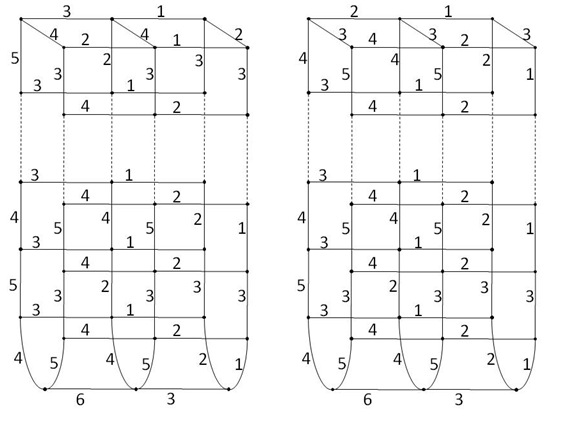
\includegraphics[width=145mm]{figures/cylinders.jpg}
\caption{$C(m,2n+1)$ գրաֆի միջակայքային 6-ներկումը, երբ $n$-ը զույգ է (ձախից) և երբ $n$-ը կենտ է (աջից)}
\label{cylinders}
\end{figure}

Այժմ ենթադրենք $m$-ը կենտ է: Սկզբում ցույց տանք, որ $C(3,2n+1)$-ը ունի միջակայքային $6$-ներկում: Սահմանենք $C(3,2n+1)$-ի $\gamma$ կողային ներկումը հետևյալ կերպ.
\begin{description}
\item[(1)]
$\gamma\left(v_{1}^{(1)}v_{1}^{(2)}\right)=6$, $\gamma\left(v_{j}^{(1)}v_{j}^{(2)}\right)=4$, որտեղ $j=2,\ldots,2\left\lfloor\frac{n+1}{2}\right\rfloor$,
\item[(2)]
$\gamma\left(v_{2\left\lfloor\frac{n+1}{2}\right\rfloor+1}^{(1)}v_{2\left\lfloor\frac{n+1}{2}\right\rfloor+1}^{(2)}\right)=2$, $\gamma\left(v_{j}^{(1)}v_{j}^{(2)}\right)=3$, որտեղ  $j=2\left\lfloor\frac{n+1}{2}\right\rfloor+2,\ldots,2n+1$,
\item[(3)]
$\gamma\left(v_{1}^{(2)}v_{1}^{(3)}\right)=3$, $\gamma\left(v_{j}^{(2)}v_{j}^{(3)}\right)=2$, որտեղ $j=2,\ldots,2\left\lfloor\frac{n+1}{2}\right\rfloor$,
\item[(4)]
$\gamma\left(v_{j}^{(2)}v_{j}^{(3)}\right)=1$, որտեղ $j=2\left\lfloor\frac{n+1}{2}\right\rfloor+1,\ldots,2n+1$,
\item[(5)]
$\gamma\left(v_{2j-1}^{(1)}v_{2j}^{(1)}\right)=\gamma\left(v_{2j-1}^{(2)}v_{2j}^{(2)}\right)=5$
և
$\gamma\left(v_{2j}^{(1)}v_{2j+1}^{(1)}\right)=\gamma\left(v_{2j}^{(2)}v_{2j+1}^{(2)}\right)=3$,

որտեղ $j=1,\ldots,\left\lfloor\frac{n+1}{2}\right\rfloor,$

\item[(6)]
$\gamma\left(v_{2j-1}^{(1)}v_{2j}^{(1)}\right)=\gamma\left(v_{2j-1}^{(2)}v_{2j}^{(2)}\right)=4$
և
$\gamma\left(v_{1}^{(1)}v_{2n+1}^{(1)}\right)=\gamma\left(v_{1}^{(2)}v_{2n+1}^{(2)}\right)=4$,

 որտեղ $j=\left\lfloor\frac{n+1}{2}\right\rfloor+1,\ldots,n$,

\item[(7)]
$\gamma\left(v_{2j}^{(1)}v_{2j+1}^{(1)}\right)=\gamma\left(v_{2j}^{(2)}v_{2j+1}^{(2)}\right)=2$, որտեղ $j=\left\lfloor\frac{n+1}{2}\right\rfloor+1,\ldots,n$,

\item[(8)]
$\gamma\left(v_{2j-1}^{(3)}v_{2j}^{(3)}\right)=1$ և $\gamma\left(v_{2j}^{(3)}v_{2j+1}^{(3)}\right)=3$, որտեղ $j=1,\ldots,\left\lfloor\frac{n+1}{2}\right\rfloor$,

\item[(9)]
$\gamma\left(v_{2j-1}^{(3)}v_{2j}^{(3)}\right)=2$ և $\gamma\left(v_{1}^{(3)}v_{2n+1}^{(3)}\right)=2$, որտեղ $j=\left\lfloor\frac{n+1}{2}\right\rfloor+1,\ldots,n$,

\item[(10)]
$\gamma\left(v_{2j}^{(3)}v_{2j+1}^{(3)}\right)=3$, որտեղ $j=\left\lfloor\frac{n+1}{2}\right\rfloor+1,\ldots,n$:
\end{description}

Դժվար չէ տեսնել, որ $\gamma$-ն $C(3,2n+1)$-ի միջակայքային $6$-ներկում է, ընդ որում՝ $S(v_{j}^{(3)},\gamma)=[1,3]$ բոլոր $1\leq
j\leq 2n+1$ թվերի համար:

Այնուհետև կառուցենք $\phi$ ներկումը $C(m,2n+1)$ գրաֆի համար: Նախ ներկենք $C(m,2n+1)$-ի $C(3,2n+1)$ ենթագրաֆի կողերը՝ համաձայն $\gamma$ ներկման: Մնացած $C(m-3,2n+1)$ ենթագրաֆը ներկենք համաձայն $\beta$ ներկման: Վերջապես, $v_{j}^{(3)}v_{j}^{(4)}\in E_{j}$ ($1\leq j\leq 2n+1$) կողերը ներկենք $4$ գույնով: Հեշտ է տեսնել, որ $\phi$-ն $C(m,2n+1)$-ի միջակայքային $6$-ներկում է: Փաստորեն, $C(m,2n+1)\in \mathfrak{N}$ և $w(C(m,2n+1))\leq 6$.

Քանի որ կենտ $m$-երի դեպքում $G=C(m,2n+1)$ գրաֆը չունի կատարյալ զուգակցում, իսկ $\delta(G)=3$, $\Delta(G)=4$, ըստ Հետևանք \ref{c1_lower_nopm}-ի՝ $w(C(m,2n+1))\geq \max\left\{\Delta(G),2\delta(G)\right\} = 6$:
\end{proof}

Այսպիսով, մեզ հաջողվեց կառուցել միջակայքային ներկումներ ինչպես ցանցերի, այնպես էլ գլանների համար: Ունենալով այդ ներկումները և հաշվի առնելով Լեմմա \ref{t2_behzad}-ը, կարող ենք ձևակերպել հետևյալ պնդումը.

\begin{theorem}
\label{t2_planars} Եթե $G\square H$ դեկարտյան արտադրյալը հարթ է, ընդ որում 2 արտադրիչներն էլ ունեն առնվազն $3$ գագաթ, ապա $G\square H\in \mathfrak{N}$ և $w(G\square H)\leq 6$:
\end{theorem}

Գլանի ներկման համար անհրաժեշտ գույների առավելագույն քանակի համար Պետրոսյանը և Կարապետյանը \cite{PetrosyanKarapetyan2007} ստացել են ստորին գնահատական այն դեպքում, երբ գլանի բաղադրիչ ցիկլի երկարությունը զույգ է.
\begin{theorem}
\label{t2_cylinder_W_evencycle} Ցանկացած $m\in \mathbb{N}, n\geq 2$ թվերի համար
\begin{center}
$W(C(m,2n))\geq 3m+n-2$:
\end{center}
\end{theorem}

Մեզ հաջողվել ստանալ գնահատական այն դեպքում, երբ գլանի բաղադրիչ շղթայի երկարությունն է զույգ:
\begin{theorem}
\label{t2_cylinder_W_evenpath} Երբ $m\in\mathbb{N},n\geq 2$, 
\begin{center}
$W(C(2m,2n))\geq 4m+2n-2$,
\end{center}
իսկ երբ $m,n\in\mathbb{N}$,
\begin{center}
$W(C(2m,2n+1))\geq 4m+2n-1$:
\end{center}
\end{theorem}
\begin{proof}[Ապացույց] Թեորեմն ապացուցելու համար բավական է կառուցել համապատասխան պայմաններին բավարարող ներկումներ: Դիցուք, 
\begin{align*}
V(C(2m,2n))&=\left\{v_{j}^{(i)}\colon\,1\leq i\leq 2m,1\leq j\leq 2n\right\},\\
V(C(2m,2n+1))&=\left\{u_{j}^{(i)}\colon\,1\leq i\leq 2m,1\leq j\leq 2n+1\right\},\\
E(C(2m,2n))&=\bigcup_{i=1}^{2m}E^{i}\cup \bigcup_{j=1}^{2n}E_{j}, \\
E(C(2m,2n+1))&=\bigcup_{i=1}^{2m}\hat{E}^{i}\cup \bigcup_{j=1}^{2n+1}\hat{E}_{j},
\end{align*}
որտեղ 
\begin{align*}
E^{i}&=\left\{v_{j}^{(i)}v_{j+1}^{(i)}\colon\,1\leq j\leq
2n-1,\right\}\cup \left\{v_{1}^{(i)}v_{2n}^{(i)}\right\},
&E_{j}&=\left\{v_{j}^{(i)}v_{j}^{(i+1)}\colon\,1\leq i\leq
2m-1\right\},\\
\hat{E}^{i}&=\left\{u_{j}^{(i)}u_{j+1}^{(i)}\colon\,1\leq j\leq
2n,\right\}\cup \left\{u_{1}^{(i)}u_{2n+1}^{(i)}\right\},
&\hat{E}_{j}&=\left\{u_{j}^{(i)}u_{j}^{(i+1)}\colon\,1\leq i\leq
2m-1\right\}:
\end{align*}

Նախ կառուցենք $\alpha$ միջակայքային ներկումը $C(2m,2n)$ գրաֆի համար, որտեղ $m\in\mathbb{N},n\geq 2$:

\begin{description}
\item[(1)] 
$\alpha\left(v_{j}^{(2i-1)}v_{j+1}^{(2i-1)}\right)=\alpha\left(v_{j}^{(2i)}v_{j+1}^{(2i)}\right)=4i+2j-4$, որտեղ $i=1,\ldots,m$, $j=1,\ldots,n$,
\item[(2)] 
$\alpha\left(v_{j}^{(2i-1)}v_{j+1}^{(2i-1)}\right)=\alpha\left(v_{j}^{(2i)}v_{j+1}^{(2i)}\right)=4i-2j+4n-1$, որտեղ $i=1,\ldots,m$, $j=n+1,\ldots,2n-1$,
\item[(3)] 
$\alpha\left(v_{1}^{(2i-1)}v_{2n}^{(2i-1)}\right)=\alpha\left(v_{1}^{(2i)}v_{2n}^{(2i)}\right)=4i-1$, որտեղ $i=1,\ldots,m$,
\item[(4)] 
$\alpha\left(v_{j}^{(2i-1)}v_{j}^{(2i)}\right)=4i+2j-5$, որտեղ $i=1,\ldots,m$, $j=1,\ldots,n$,
\item[(5)] 
$\alpha\left(v_{j}^{(2i-1)}v_{j}^{(2i)}\right)=4i-2j+4n$, որտեղ $i=1,\ldots,m$, $j=n+1,\ldots,2n$,
\item[(6)] 
$\alpha\left(v_{j}^{(2i)}v_{j}^{(2i+1)}\right)=4i+2j-3$, որտեղ $i=1,\ldots,m-1$, $j=2,\ldots,n+1$,
\item[(7)] 
$\alpha\left(v_{j}^{(2i)}v_{j}^{(2i+1)}\right)=4i-2j+4n+2$, որտեղ $i=1,\ldots,m-1$, $j=n+2,\ldots,2n$,
\item[(8)] 
$\alpha\left(v_{1}^{(2i)}v_{1}^{(2i+1)}\right)=4i$, որտեղ $i=1,\ldots,m-1$:
\end{description}

Այժմ կառուցենք $\beta$ ներկումը $C(2m,2n+1)$ գրաֆի համար, որտեղ $m,n\in\mathbb{N}$:

\begin{description}
\item[(1)] 
$\beta\left(u_{j}^{(2i-1)}u_{j+1}^{(2i-1)}\right)=\beta\left(u_{j}^{(2i)}u_{j+1}^{(2i)}\right)=4i+2j-4$, որտեղ $i=1,\ldots,m$, $j=1,\ldots,n+1$,
\item[(2)] 
$\beta\left(u_{j}^{(2i-1)}u_{j+1}^{(2i-1)}\right)=\beta\left(u_{j}^{(2i)}u_{j+1}^{(2i)}\right)=4i-2j+4n+1$, որտեղ $i=1,\ldots,m$, $j=n+2,\ldots,2n$,
\item[(3)] 
$\beta\left(u_{1}^{(2i-1)}u_{2n+1}^{(2i-1)}\right)=\beta\left(u_{1}^{(2i)}u_{2n+1}^{(2i)}\right)=4i-1$, որտեղ $i=1,\ldots,m$,
\item[(4)] 
$\beta\left(u_{j}^{(2i-1)}u_{j}^{(2i)}\right)=4i+2j-5$, որտեղ $i=1,\ldots,m$, $j=1,\ldots,n+2$,
\item[(5)] 
$\beta\left(u_{j}^{(2i-1)}u_{j}^{(2i)}\right)=4i-2j+4n+2$, որտեղ $i=1,\ldots,m$, $j=n+3,\ldots,2n+1$,
\item[(6)] 
$\beta\left(u_{j}^{(2i)}u_{j}^{(2i+1)}\right)=4i+2j-3$, որտեղ $i=1,\ldots,m-1$, $j=2,\ldots,n+1$,
\item[(7)] 
$\beta\left(u_{j}^{(2i)}u_{j}^{(2i+1)}\right)=4i-2j+4n+4$, որտեղ $i=1,\ldots,m-1$, $j=n+2,\ldots,2n+1$,
\item[(8)] 
$\beta\left(u_{1}^{(2i)}u_{1}^{(2i+1)}\right)=4i$, որտեղ $i=1,\ldots,m-1$:
\end{description}

Դժվար չէ ստուգել, որ $\alpha$-ն $C(2m,2n)$-ի միջակայքային $(4m+2n-2)$-ներկում է, երբ $m\in\mathbb{N},n\geq 2$,
իսկ $\beta$-ն $C(2m,2n+1)$-ի միջակայքային $(4m+2n-1)$-ներկում է, երբ $m,n\in\mathbb{N}$:
\end{proof}

Նկատենք, որ երբ գլանի երկու բաղադրիչներն էլ ունեն զույգ թվով գագաթներ, \ref{t2_cylinder_W_evencycle} և \ref{t2_cylinder_W_evenpath} թեորեմները տալիս են տարբեր ստորին գնահատականներ $W\left(C(2m,2n)\right)$-ի համար: Երբ $n>2m$, Թեորեմ \ref{t2_cylinder_W_evenpath}-ի գնահատականը ավելի լավն է: Երբ $n=2m$, երկու թեորեմներն էլ տալիս են նույն գնահատականը: Իսկ երբ $n<2m$ ավելի լավն է Թեորեմ \ref{t2_cylinder_W_evencycle}-ի գնահատականը:

Թեորեմ \ref{t2_cylinder_W_evenpath}-ի ստորին գնահատականները հեռու չեն $W\left(C(2m,n)\right)$-ի համար հայտնի վերին գնահատականներից: Այսպես, քանի որ $C(2m,2n)$-ը երկկողմանի է, ընդ որում $3\leq \Delta\left(C(2m,2n)\right)\leq 4$ և $\mathrm{diam}\left(C(2m,2n)\right)=2m+n-1$, ապա Թեորեմ \ref{t1_upper_bipartite}-ից՝ $W\left(C(2m,2n)\right)\leq 3(2m+n-1)+1$: Նմանապես, քանի որ $3\leq \Delta\left(C(2m,2n+1)\right)\leq 4$ և $\mathrm{diam}\left(C(2m,2n+1)\right)=2m+n-1$, ապա Թեորեմ \ref{t1_upper}-ից՝ $W\left(C(2m,2n+1)\right)\leq 3(2m+n)+1$:


\subsubsection{Արտաքին հարթ գրաֆների ներկումներ}
\label{section_outerplanar}
Ինչպես տեսանք, $G\square H$ դեկարտյան արտադրյալը հարթ է նաև այն դեպքում, երբ $G=K_2$, իսկ $H$ գրաֆը արտաքին հարթ է: Մյուս կողմից, ըստ Թեորեմ \ref{t2_cartesian_gap}-ի, $G \square H$ արտադրյալը ունի միջակայքային ներկում այն և միայն դեպքում, երբ $H$-ը ունի միջակայքային մեկ անցքով ներկում: Այս պարագրաֆում կնկարագրենք արտաքին հարթ գրաֆների հատուկ տիպի ներկման կառուցման ալգորիթմ, որի շնորհիվ ցույց կտրվի, որ արտաքին հարթ գրաֆները բավարարում են Հիպոթեզ \ref{conj_def}-ին, իսկ եռանկյուն չպարունակող արտաքին գրաֆները նաև միջակայքային $1$-անցք-ներկելի են:

Ֆիորինին \cite{Fiorini1975} նկարագրել է բոլոր արտաքին հարթ գրաֆների քրոմատիկ դասը.
\begin{theorem}
Եթե $G$-ն արտաքին հարթ գրաֆ է, ապա $\chi'(G)=\Delta(G) + 1$ այն և միայն այն դեպքում, երբ $G$-ն կենտ ցիկլ է:
\end{theorem}

Թեորեմ \ref{t1_class1}-ից անմիջապես հետևում է, որ կենտ ցիկլերը միջակայքային ներկելի չեն: Սակայն գոյություն ունեն բազմաթիվ այլ արտաքին հարթ գրաֆներ, որոնց դեֆիցիտը դրական է: Օրինակ, Նկ. \ref{outerplanar-non-colorable}-ում պատկերված գրաֆը էյլերյան է, ունի կենտ թվով կողեր, և համաձայն Հետևանք \ref{c1_eulerian}-ի՝ չի կարող ունենալ միջակայքային ներկում: Մյուս կողմից, հեշտ է տեսնել, որ այդ գրաֆն ունի $1$ դեֆիցիտով ներկում:

\begin{figure}
  \begin{center}
  \begin{tikzpicture}[style=thick]
    \draw (90:1.4cm) -- node [right] {$3$}  
    (-30:1.4cm) -- node [sloped,above] {$4$} 
    (-150:1.4cm) -- node [left] {$1$} cycle;
    \draw (90:1.4cm) -- node [sloped,above] {$2$}  
    (150:1.7cm) -- node [left] {$3$}  
    (-150:1.4cm) -- node [sloped,below] {$2$}  
    (-90:1.7cm) -- node [sloped,below] {$1$}  
    (-30:1.4cm) -- node [right] {$5$} 
    (30:1.7cm) -- node [sloped,above] {$4$} cycle;
    
    \draw[fill=black] (90:1.4cm) circle (2pt);
    \draw[fill=white,style=ultra thick] (-30:1.4cm) circle (3pt);
    \draw[fill=black] (-150:1.4cm) circle (2pt);
    \draw[fill=black] (150:1.7cm) circle (2pt);
    \draw[fill=black] (-90:1.7cm) circle (2pt);
    \draw[fill=black] (30:1.7cm) circle (2pt);
  \end{tikzpicture}
  \end{center}
  \caption{Արտաքին հարթ տրիանգուլյացիա, որը միջակայքային ներկելի չէ: Պատկերված ներկման դեֆիցիտը $1$ է:}
  \label{outerplanar-non-colorable}
\end{figure}

Հայտնի է, որ արտաքին հարթ գրաֆների որոշ ենթադասեր միջակայքային ներկելի են: Արտաքին հարթ գրաֆը կոչվում է արտաքին հարթ տրիանգուլյացիա, եթե այն կարելի է պատկերել հարթության վրա այնպես, որ բոլոր սահմանափակ նիստերը լինեն եռանկյուն: Հարթության վրա պատկերված արտաքին հարթ գրաֆի եռանկյուն նիստը կոչվում է բաժանող եռանկյուն, եթե նրա կողմերից ոչ մեկը չի պատկանում անվերջ նիստին: Աքսենովիչը \cite{Axenovich2002} ապացուցել է հետևյալ թեորեմը.

\begin{theorem}
Եթե $G$-ն առնվազն չորս գագաթ պարունակող արտաքին հարթ տրիանգուլյացիա է և չունի բաժանող եռանկյուն, ապա այն միջակայքային ներկելի է:
\end{theorem}

Նկ. \ref{outerplanar-non-colorable}-ում պատկերված գրաֆը բաժանող եռանկյուն պարունակող արտաքին հարթ տրիանգուլյացիա է և չունի միջակայքային ներկում:

Հետագայում, Գիառոն և Կուբալեն \cite{GiaroKubale2004} նկարագրել են արտաքին հարթ գրաֆների միջակայքային ներկելի ևս մեկ ենթադաս.
\begin{theorem}
\label{t2_bipartite_outerplanar}
Եթե $G$-ն երկկողմանի արտաքին հարթ գրաֆ է, ապա այն միջակայքային ներկելի է:
\end{theorem}

Վերջապես, Պետրոսյանը \cite{Petrosyan2013Outerplanar} ստացել է հետևյալ արդյունքը.
\begin{theorem}
Եթե $G$-ն կապակցված ենթախորանարդ արտաքին հարթ գրաֆ է, բացի կենտ ցիկլից, ապա այն միջակայքային ներկելի է:
\end{theorem}

Այս պարագրաֆում մենք կդիտարկենք բոլոր արտաքին հարթ գրաֆների դեֆիցիտը և կընդհանրացնենք Թեորեմ  \ref{t2_bipartite_outerplanar}-ը:

$f_i(G)$-ով նշանակենք հարթության վրա պատկերված $G$ արտաքին հարթ գրաֆում $i$ կողեր ունեցող սահմանափակ նիստերի քանակը, որտեղ $i=3,4,\ldots,|V(G)|$:

\begin{lemma}
\label{outerplanar_basic_2connected}
Եթե $G$-ն համիլտոնյան արտաքին հարթ գրաֆ է, իսկ $w_0 \in V(G)$-ն այդ գրաֆի որևէ ֆիքսված գագաթ, ապա գոյություն ունի $G$-ի $\alpha$ ճիշտ կողային ներկում այնպիսին, որ.
\begin{itemize}
\item $def(w_0,\alpha)=0$,
\item $def(G,\alpha)=\sum\limits_{\substack{i\geq 3 \\ \text{կենտ }i}}{f_i(G)}$,
\item $gn(G,\alpha) \leq f_3(G) + \min\left\{1, \sum\limits_{\substack{i\geq 5 \\ \text{կենտ }i}}{f_{i}(G)}]\right\}$:
\end{itemize}
\end{lemma}
\begin{proof}[Ապացույց]
Այս լեմմայի ապացույցը ընդլայնում է \cite{DeWerraSolot1991}-ի Պնդում 3.1-ում և \cite{GiaroKubale2004}-ի Թեորեմ 2.3-ում մշակված մեթոդը:

Դիցուք $|V(G)|=n$ և $G$-ն պատկերված է հարթության վրա այնպես, որ բոլոր գագաթները պատկանում են անվերջ նիստին: $\alpha$ ներկումը կառուցելու ենք զուգահեռաբար ներկելով և նշելով $G$-ի կողերը: Կողերի նշումների ֆունկցիան նշանակենք $\lambda$-ով. $\lambda : E(G) \rightarrow \left\{\bm{l},\bm{u},\bm{m}\right\}$: Ալգորիթմի յուրաքանչյուր քայլում դիտարկվում է $G$-ի մեկ նիստ և, նիստին պատկանող կողերից մեկի նախապես որոշված գույնի և նշման հիման վրա միարժեքորեն որոշվում են մյուս կողերի գույները և նշումները: Նիստերի դիտարկման հերթականությունը որոշվում է ըստ $G$-ի $T$ թույլ երկակի գրաֆի: $T$-ի գագաթները համապատասխանում են $G$-ի սահմանափակ նիստերին և երկու գագաթներ միացած են կողով այն և միայն դեպքում, երբ համապատասխան նիստերը $G$-ում ունեն ընդհանուր կող: Հայտնի է, որ արտաքին հարթի թույլ երկակի գրաֆը անտառ է \cite{Harary1974}: Մեր դեպքում $G$-ն համիլտոնյան է, ուստի $2$-կապակցված է, հետևաբար թույլ երկակի գրաֆը ծառ է: Ստորև տրված է $\alpha$-ն և $\lambda$-ն կառուցող ալգորիթմի նկարագրությունը:

\begin{enumerate}
\item Պատկերենք $G$ գրաֆը հարթության վրա առանց խաչումների այնպես, որ բոլոր գագաթները պատկանեն անվերջ նիստին: Անվերջ նիստի կողերը կազմում են համիլտոնյան ցիկլ: Գրաֆի գագաթաները համակարալենք սկսած $w_0$-ից այդ ցիկլի երկայնքով ժամացույցի սլաքի ուղղությամբ. $w_0, w_1, \ldots, w_{n-1}$:
\item Կառուցենք $G$-ի $T$ թույլ երկակի գրաֆը:
\item Վերցնենք $G$-ի այն նիստը, որը պարունակում է $w_0w_{n-1}$ կողը: Դիցուք $t_0 \in V(T)$ գագաթը համապատասխանում է այդ նիստին: Նկատենք, որ այս նիստը միարժեք է որոշվում, քանի որ հակառակ դեպքում $w_0w_{n-1}$ կողը չէր պատկանի անվերջ նիստին: Դիցուք այդ նիստին պատկանող գագաթներն են $w_0=v_1,v_2,\ldots,v_r=w_{n-1}$ (ժամացույցի սլաքի ուղղությամբ):
\item Վերցնենք $\alpha(v_1v_r) = 1$ և $\lambda(v_1v_r)=\bm{u}$: \label{algo_set_first}
\item Լայնությամբ շրջանցենք $T$ ծառը՝ սկսելով $t_0$ գագաթից: Դիցուք $F$-ը $G$-ի այն նիստն է, որը համապատասխանում է տվյալ պահին դիտարկվող $t \in V(T)$ գագաթին: Ալգորիթմը երաշխավորում է, որ $F$-ի կողերից մեկը նախորդ քայլերից մեկում արդեն ներկվել և նշվել է: Դիցուք $V(F) = \left\{v_1,v_2,\ldots,v_r\right\}$ (ժամացույցի սլաքի ուղղությամբ), որտեղ $v_1v_r$-ը նախորդ քայլերից մեկում նշված կողն է և $\alpha(v_1v_r)=k$: Մնացած կողերի գույներն ու նշումները որոշվում են կախված $r$-ից և $\lambda(v_1v_r)$ նշումից (Նկ. \ref{outerplanar_figures}): \label{algo_traverse}
	\begin{enumerate}
    \item Եթե $\lambda(v_1v_r)=\bm{l}$, ապա ալգորիթմը երաշխավորում է, որ $\underline{S}(v_1, \alpha) = \underline{S}(v_r, \alpha) = k$, ուստի ներկումը կմնա ճիշտ, եթե նոր կողերին վերագրենք ավելի փոքր գույներ:
    	\begin{enumerate}
    	\item Եթե $r=3$, ապա վերցնենք $\alpha(v_1v_2)=k-1$, $\alpha(v_2v_3)=k-2$, $\lambda(v_1v_2)=\bm{m}$ և $\lambda(v_2v_3)=\bm{l}$: Նկատենք, որ $k-1$ գույնը բացակայում է $v_3$ գագաթի սպեկտրից և ալգորիթմի հաջորդ քայլերի ընթացքում ևս այդ գույնը չի օգտագործվի: \label{step3l}
        \item Եթե $r=2s$, $s\geq 2$, ապա $v_1v_2, v_2v_3, ..., v_{2s-1}v_{2s}$ կողերը ներկենք հերթականորեն $k-1$ և $k$ գույներով և նշենք հերթականորեն $\bm{l}$-ով և $\bm{u}$-ով: \label{step4l}
        \item Եթե $r=2s+1$, $s\geq 2$, ապա վերցնենք $\alpha(v_1v_2)=k-1$, $\alpha(v_2v_3)=k-2$, $\lambda(v_1v_2)=\bm{m}$, $\lambda(v_2v_3)=\bm{l}$, իսկ $v_3v_4, v_4v_5, ..., v_{2s}v_{2s+1}$ կողերը ներկենք հերթականորեն $k$ և $k-1$ գույներով և նշենք հերթականորեն $\bm{u}$-ով և $\bm{l}$-ով: Նկատենք, որ $v_3$ գագաթի սպեկտրից կբացակայի $k-1$ գույնը:\label{step5l}
    	\end{enumerate}
    
    \item Եթե $\lambda(v_1v_r)=\bm{u}$, ապա ալգորիթմը երաշխավորում է, որ $\overline{S}(v_1, \alpha) = \overline{S}(v_r, \alpha) = k$, ուստի ներկումը կմնա ճիշտ, եթե նոր կողերի վրա օգտագործենք ավելի մեծ գույներ:
    	\begin{enumerate}
    	\item Եթե $r=3$, ապա վերցնենք $\alpha(v_1v_2)=k+1$, $\alpha(v_2v_3)=k+2$, $\lambda(v_1v_2)=\bm{m}$ և $\lambda(v_2v_3)=\bm{u}$: Նկատենք, որ $v_3$ գագաթի սպեկտրից կբացակայի $k+1$ գույնը: \label{step3u}
        \item Եթե $r=2s$, $s\geq 2$, ապա $v_1v_2, v_2v_3, ..., v_{2s-1}v_{2s}$ կողերը ներկենք հերթականորեն $k-1$ և $k$ գույներով և նշենք հերթականորեն $\bm{u}$-ով և $\bm{l}$-ով: \label{step4u}
        \item Եթե $r=2s+1$, $s\geq 2$, ապա վերցնենք $\alpha(v_1v_2)=k+1$, $\alpha(v_2v_3)=k+2$, $\lambda(v_1v_2)=\bm{m}$, $\lambda(v_2v_3)=\bm{u}$, իսկ $v_3v_4, v_4v_5, ..., v_{2s}v_{2s+1}$ կողերը ներկենք հերթականորեն $k$ և $k+1$ գույներով և նշենք հերթականորեն $\bm{l}$-ով և $\bm{u}$-ով: Նկատենք, որ $v_3$ գագաթի սպեկտրում չի մասնակցի $k+1$ գույնը:\label{step5u}
    	\end{enumerate}
    \item Եթե $\lambda(v_1v_r)=\bm{m}$, ապա ալգորիթմը երաշխատվորում է, որ կա՛մ $\overline{S}(v_1,\alpha) = \underline{S}(v_r,\alpha) = k$, կա՛մ $\underline{S}(v_1,\alpha) = \overline{S}(v_r,\alpha) = k$:
    	\begin{enumerate}
    	\item Եթե $\underline{S}(v_1,\alpha) = \overline{S}(v_r,\alpha) = k$, ապա $F$ նիստի գագաթները վերահամարակալենք ժամացույցի սլաքի հակառակ ուղղությամբ՝ այսպիսով երաշխավորելով, որ $\overline{S}(v_1,\alpha) = \underline{S}(v_r,\alpha) = k$: \label{stepmrename}
        \item Եթե $r=3$, ապա վերցնենք $\alpha(v_1v_2)=k+1$, $\alpha(v_2v_3)=k-1$, $\lambda(v_1v_2)=\bm{u}$ և $\lambda(v_2v_3)=\bm{l}$: Նկատենք, որ $v_2$ գագաթի սպեկտրում չի մասնակցի $k$ գույնը: \label{step3m}
        \item Եթե $r=2s$, $s\geq 2$, ապա վերցնենք $\alpha(v_1v_2)=k+1$, $\alpha{v_2v_3} = k$, $\lambda(v_1v_2)=\bm{u}$ և $\lambda(v_2v_3)=\bm{m}$: Այնուհետև $v_3v_4, v_4v_5, ..., v_{2s-1}v_{2s}$ կողերը ներկենք հերթականորեն $k-1$ և $k$ գույներով և նշենք հերթականորեն $\bm{u}$-ով և $\bm{l}$-ով: \label{step4m}
        \item Եթե $r=2s+1$, $s\geq 2$, ապա վերցնենք $\alpha(v_1v_2)=k+1$, $\lambda(v_1v_2)=\bm{u}$, իսկ $v_2v_3, v_3v_4, ..., v_{2s}v_{2s+1}$ կողերը ներկենք հերթականորեն $k-1$ և $k$ գույներով և նշենք հերթականորեն $\bm{l}$-ով և $\bm{u}$-ով:\label{step5m}
    	\end{enumerate}
	\end{enumerate}
    \item Եթե $\min_{e \in E(G)}\alpha(e) = c_0 \ne 1$, ապա բոլոր կողերի գույները շեղենք համաձայն $\alpha(e) = \alpha(e) - c_0 + 1$ ($e \in E(G)$), բանաձևի:
\end{enumerate}

\begin{figure}
\tikzset{font=\fontsize{9pt}{12}}
\begin{tabular}{|m{.024\textwidth}| m{.22\textwidth} | m{.287\textwidth} | m{.334\textwidth}|}
\hline
 & $r=3$ & $r=2s$, $s\geq 2$ & $r=2s+1$, $s\geq 2$ \\
\hline
$\bm{l}$ & 
  \begin{tikzpicture}[style=thick]
    \draw (120:1.3cm) -- node [sloped,above] {$k-1$} node [sloped,below, fill=white] {$\bm{m}$} (0:1.3cm) -- node [sloped,above] {$\bm{l}$} node [sloped,below] {$k-2$} (240:1.3cm);
    
    \draw (120:2.3cm) -- node [right,sloped,near start,rotate=90] {$>k$}
    (120:1.3cm) -- node [left] {$k$} node [right] {$\bm{l}$} 
    (-120:1.3cm) -- node [right,sloped,near end,rotate=-90] {$>k$}
    (-120:2.3cm);
    
    \draw[fill=black] (120:1.3cm) circle (2pt) node [left] {$v_1$};
    \draw[fill=black] (0:1.3cm) circle (2pt) node [below] {$v_2$};
    \draw[fill=white,style=ultra thick] (-120:1.3cm) circle (3pt) node [left] {$v_3$};
  \end{tikzpicture} & 
  
  
  \begin{tikzpicture}[style=thick]
    \draw (150:1.4cm) -- node [sloped,above] {$k-1$} node [sloped,below] {$\bm{l}$} 
    (90:1.4cm) -- node [sloped,above] {$k$} node [sloped,below] {$\bm{u}$} 
    (30:1.4cm) -- node [sloped,above] {$k-1$} node [left] {$\bm{l}$} 
    (-30:1.4cm);
    \draw (-30:1.4cm) -- 
    (-90:1.4cm) [dashed];
    \draw (-90:1.4cm) -- node [sloped,below] {$k-1$} node [sloped,above] {$\bm{l}$} 
    (-150:1.4cm);
    
    \draw (135:2.7cm) -- node [right,sloped,near start,rotate=90] {$>k$}
    (150:1.4cm) -- node [left] {$k$} node [right] {$\bm{l}$} 
    (-150:1.4cm) -- node [right,sloped,near end,rotate=-90] {$>k$}
    (-135:2.7cm);
    
    \draw[fill=black] (150:1.4cm) circle (2pt) node [left] {$v_1$};
    \draw[fill=black] (90:1.4cm) circle (2pt) node [above] {$v_2$};
    \draw[fill=black] (30:1.4cm) circle (2pt) node [right] {$v_3$};
    \draw[fill=black] (-30:1.4cm) circle (2pt);
    \draw[fill=black] (-90:1.4cm) circle (2pt) node [below] {$v_{2s-1}$};
    \draw[fill=black] (-150:1.4cm) circle (2pt) node [left] {$v_{2s}$};
  \end{tikzpicture} & 
  
  
  \begin{tikzpicture}[style=thick]
    \draw (156:1.4cm) -- node [sloped,above] {$k-1$} node [sloped,below] {$\bm{m}$} 
    (104:1.4cm) -- node [sloped,above] {$k-2$} node [sloped,below] {$\bm{l}$} 
    (52:1.4cm) -- node [sloped,above] {$k$} node [sloped,below] {$\bm{u}$} 
    (0:1.4cm) -- node [sloped,below] {$k-1$} node [sloped,above] {$\bm{l}$} 
    (-52:1.4cm);
    \draw (-52:1.4cm) -- 
    (-104:1.4cm) [dashed];
    \draw (-104:1.4cm) -- node [sloped,above] {$\bm{l}$} node [sloped,below] {$k-1$} 
    (-156:1.4cm);
    
    \draw (135:2.7cm) -- node [right,sloped,near start,rotate=90] {$>k$}
    (156:1.4cm) -- node [left] {$k$} node [right] {$\bm{l}$} 
    (-156:1.4cm) -- node [right,sloped,near end,rotate=-90] {$>k$}
    (-135:2.7cm);
    
    \draw[fill=black] (156:1.4cm) circle (2pt) node [left] {$v_1$};
    \draw[fill=black] (104:1.4cm) circle (2pt) node [above] {$v_2$};
    \draw[fill=white,style=ultra thick] (52:1.4cm) circle (3pt) node [right] {$v_3$};
    \draw[fill=black] (0:1.4cm) circle (2pt) node [right] {$v_4$};
    \draw[fill=black] (-52:1.4cm) circle (2pt);
    \draw[fill=black] (-104:1.4cm) circle (2pt) node [below] {$v_{2s}$};
    \draw[fill=black] (-156:1.4cm) circle (2pt) node [left] {$v_{2s+1}$};
  \end{tikzpicture} \\
\hline


$\bm{u}$ & 
  \begin{tikzpicture}[style=thick]
    \draw (120:1.3cm) -- node [sloped,above] {$k+1$} node [sloped,below] {$\bm{m}$} (0:1.3cm) -- node [sloped,above] {$\bm{u}$} node [sloped,below] {$k+2$} (240:1.3cm);
    
    \draw (120:2.3cm) -- node [right,sloped,near start,rotate=90] {$<k$}
    (120:1.3cm) -- node [left] {$k$} node [right] {$\bm{u}$} 
    (-120:1.3cm) -- node [right,sloped,near end,rotate=-90] {$<k$}
    (-120:2.3cm);
    
    \draw[fill=black] (120:1.3cm) circle (2pt) node [left] {$v_1$};
    \draw[fill=black] (0:1.3cm) circle (2pt) node [below] {$v_2$};
    \draw[fill=white,style=ultra thick] (-120:1.3cm) circle (3pt) node [left] {$v_3$};
  \end{tikzpicture} & 
  
  
  \begin{tikzpicture}[style=thick]
    \draw (150:1.4cm) -- node [sloped,above] {$k+1$} node [sloped,below] {$\bm{u}$} 
    (90:1.4cm) -- node [sloped,above] {$k$} node [sloped,below] {$\bm{l}$} 
    (30:1.4cm) -- node [sloped,above] {$k+1$} node [left] {$\bm{u}$} 
    (-30:1.4cm);
    \draw (-30:1.4cm) -- 
    (-90:1.4cm) [dashed];
    \draw (-90:1.4cm) -- node [sloped,below] {$k+1$} node [sloped,above] {$\bm{u}$} 
    (-150:1.4cm);
    
    \draw (135:2.7cm) -- node [right,sloped,near start,rotate=90] {$<k$}
    (150:1.4cm) -- node [left] {$k$} node [right] {$\bm{u}$} 
    (-150:1.4cm) -- node [right,sloped,near end,rotate=-90] {$<k$}
    (-135:2.7cm);
   
    \draw[fill=black] (150:1.4cm) circle (2pt) node [left] {$v_1$};
    \draw[fill=black] (90:1.4cm) circle (2pt) node [above] {$v_2$};
    \draw[fill=black] (30:1.4cm) circle (2pt) node [right] {$v_3$};
    \draw[fill=black] (-30:1.4cm) circle (2pt);
    \draw[fill=black] (-90:1.4cm) circle (2pt) node [below] {$v_{2s-1}$};
    \draw[fill=black] (-150:1.4cm) circle (2pt) node [left] {$v_{2s}$};
  \end{tikzpicture} & 
  
  
  \begin{tikzpicture}[style=thick]
    \draw (156:1.4cm) -- node [sloped,above] {$k+1$} node [sloped,below] {$\bm{m}$} 
    (104:1.4cm) -- node [sloped,above] {$k+2$} node [sloped,below] {$\bm{u}$} 
    (52:1.4cm) -- node [sloped,above] {$k$} node [sloped,below] {$\bm{l}$} 
    (0:1.4cm) -- node [sloped,below] {$k+1$} node [sloped,above] {$\bm{u}$} 
    (-52:1.4cm);
    \draw (-52:1.4cm) -- 
    (-104:1.4cm) [dashed];
    \draw (-104:1.4cm) -- node [sloped,below] {$k+1$} node [sloped,above] {$\bm{u}$} 
    (-156:1.4cm);
    
    \draw (135:2.7cm) -- node [right,sloped,near start,rotate=90] {$<k$}
    (156:1.4cm) -- node [left] {$k$} node [right] {$\bm{u}$} 
    (-156:1.4cm) -- node [right,sloped,near end,rotate=-90] {$<k$}
    (-135:2.7cm);
    
    \draw[fill=black] (156:1.4cm) circle (2pt) node [left] {$v_1$};
    \draw[fill=black] (104:1.4cm) circle (2pt) node [above] {$v_2$};
    \draw[fill=white,style=ultra thick] (52:1.4cm) circle (3pt) node [right] {$v_3$};
    \draw[fill=black] (0:1.4cm) circle (2pt) node [right] {$v_4$};
    \draw[fill=black] (-52:1.4cm) circle (2pt);
    \draw[fill=black] (-104:1.4cm) circle (2pt) node [below] {$v_{2s}$};
    \draw[fill=black] (-156:1.4cm) circle (2pt) node [left] {$v_{2s+1}$};
  \end{tikzpicture} \\
\hline


$\bm{m}$ & 
  \begin{tikzpicture}[style=thick]
    \draw (120:1.3cm) -- node [sloped,above] {$k+1$} node [sloped,below, fill=white] {$\bm{u}$} (0:1.3cm) -- node [sloped,above] {$\bm{l}$} node [sloped,below] {$k-1$} (240:1.3cm);
    
    \draw (120:2.3cm) -- node [right,sloped,near start,rotate=90] {$<k$}
    (120:1.3cm) -- node [left] {$k$} node [right] {$\bm{m}$} 
    (-120:1.3cm) -- node [right,sloped,near end,rotate=-90] {$>k$}
    (-120:2.3cm);
    
    \draw[fill=black] (120:1.3cm) circle (2pt) node [left] {$v_1$};
    \draw[fill=white,style=ultra thick] (0:1.3cm) circle (3pt) node [below] {$v_2$};
    \draw[fill=black] (-120:1.3cm) circle (2pt) node [left] {$v_3$};
  \end{tikzpicture} & 
  
  
  \begin{tikzpicture}[style=thick]
    \draw (150:1.4cm) -- node [sloped,above] {$k+1$} node [sloped,below] {$\bm{u}$} 
    (90:1.4cm) -- node [sloped,above] {$k$} node [sloped,below] {$\bm{m}$} 
    (30:1.4cm) -- node [sloped,above] {$k-1$} node [left] {$\bm{l}$} 
    (-30:1.4cm);
    \draw (-30:1.4cm) -- 
    (-90:1.4cm) [dashed];
    \draw (-90:1.4cm) -- node [sloped,above] {$\bm{l}$} node [sloped,below] {$k-1$} 
    (-150:1.4cm);
    
    \draw (135:2.7cm) -- node [right,sloped,near start,rotate=90] {$<k$}
    (150:1.4cm) -- node [left] {$k$} node [right] {$\bm{m}$} 
    (-150:1.4cm) -- node [right,sloped,near end,rotate=-90] {$>k$}
    (-135:2.7cm);
    
    \draw[fill=black] (150:1.4cm) circle (2pt) node [left] {$v_1$};
    \draw[fill=black] (90:1.4cm) circle (2pt) node [above] {$v_2$};
    \draw[fill=black] (30:1.4cm) circle (2pt) node [right] {$v_3$};
    \draw[fill=black] (-30:1.4cm) circle (2pt);
    \draw[fill=black] (-90:1.4cm) circle (2pt) node [below] {$v_{2s-1}$};
    \draw[fill=black] (-150:1.4cm) circle (2pt) node [left] {$v_{2s}$};
  \end{tikzpicture} & 
  \begin{tikzpicture}[style=thick]
    \draw (156:1.4cm) -- node [sloped,above] {$k+1$} node [sloped,below] {$\bm{u}$} 
    (104:1.4cm) -- node [sloped,above] {$k-1$} node [sloped,below] {$\bm{l}$} 
    (52:1.4cm) -- node [sloped,above] {$k$} node [sloped,below] {$\bm{u}$} 
    (0:1.4cm) -- node [sloped,below] {$k-1$} node [sloped,above] {$\bm{l}$} 
    (-52:1.4cm);
    \draw (-52:1.4cm) -- 
    (-104:1.4cm) [dashed];
    \draw (-104:1.4cm) -- node [sloped,above] {$\bm{l}$} node [sloped,below] {$k-1$} 
    (-156:1.4cm);
    
    \draw (138:2.7cm) -- node [right,sloped,near start,rotate=90] {$<k$}
    (156:1.4cm) -- node [left] {$k$} node [right] {$\bm{m}$} 
    (-156:1.4cm) -- node [right,sloped,near end,rotate=-90] {$>k$}
    (-138:2.7cm);
    
    \draw[fill=black] (156:1.4cm) circle (2pt) node [left] {$v_1$};
    \draw[fill=white,style=ultra thick] (104:1.4cm) circle (3pt) node [above] {$v_2$};
    \draw[fill=black] (52:1.4cm) circle (2pt) node [right] {$v_3$};
    \draw[fill=black] (0:1.4cm) circle (2pt) node [right] {$v_4$};
    \draw[fill=black] (-52:1.4cm) circle (2pt);
    \draw[fill=black] (-104:1.4cm) circle (2pt) node [below] {$v_{2s}$};
    \draw[fill=black] (-156:1.4cm) circle (2pt) node [left] {$v_{2s+1}$};
  \end{tikzpicture} \\
\hline
\end{tabular}

\tikzset{font=\small}
\caption{Լեմմա \ref{outerplanar_basic}-ում նկարագրված ալգորիթմի Քայլ \ref{algo_traverse}-ի նկարագրությունը: Աղյուսակի տողերը համապատասխանում են $v_1v_r$ կողի նշմանը: Սյուները համապատասխանում են հերթական $F$ նիստի կողերի քանակին: Օղակներով նշված գագաթները (ի տարբերություն շրջաններով նշվածների) ցույց են տալիս, որ ալգորիթմի տվյալ քայլի արդյունքում այդ գագաթի սպեկտրներում չօգտագործված գույների քանակը (դեֆիցիտը) կավելանա մեկով:}
\label{outerplanar_figures}
\end{figure}

Ապացույցն ավարտելու համար անհրաժեշտ է ստուգել լեմմայի երեք պնդումները: Նախ, նկատենք, որ ալգորիթմը կենտ թվով կողեր ունեցող յուրաքանչյուր նիստի գագաթներից մեկի սպեկտրում ավելացնում է ճիշտ մեկ չօգտագործված գույն (\ref{step3l}, \ref{step3u}, \ref{step3m}, \ref{step5l}, \ref{step5u} և \ref{step5m} քայլերում): Ավելին, ալգորիթմը չի ավելացնում նոր չօգտագործված գույն զույգ թվով կողեր ունեցող նիստի գագաթներում (\ref{step4l}, \ref{step4u}, \ref{step4m} քայլերում): Այստեղից հետևում է, որ բոլոր գագաթների սպեկտրներում բացակայող գույների քանակը հավասար է կենտ կողեր ունեցող նիստերի քանակին. $def(G,\alpha) = \sum_{i\geq 3,\text{կենտ }i}{f_i(G)}$:

Այնուհետև, կարևոր է նկատել, որ որևէ գագաթի դեֆիցիտը մեկից մեծ կլինի միայն այն դեպքում, երբ ալգորիթմը այդ գագաթում բացակայող գույն ավելացնի այդ գագաթը պարունակող մեկից ավելի իրարից տարբեր նիստեր դիտարկելու ընթացքում: Երբ $r \geq 5$ (\ref{step5l}, \ref{step5u} և \ref{step5m} քայլեր) կամ երբ $r=3$ և $\lambda(v_1v_3)=\bm{m}$ (Քայլ \ref{step3m}), բացակայող գույնը ավելացվում է այնպիսի գագաթներում, որոնք նախորդ քայլերում չեն դիտարկվել: Ուստի գագաթի դեֆիցիտը կարող է դառնալ մեկից ավել միայն \ref{step3l} և \ref{step3u} քայլերի դեպքում ($r=3$, և $\lambda(v_1v_r)=\bm{l}$ կամ $\lambda(v_1v_r)=\bm{u}$): Այսպիսով, կամայական գագաթի դեֆիցիտը չի կարող լինել $G$-ում եռանկյունների քանակին գումարած մեկ թվից, այն դեպքում, երբ այն պատկանում է նաև ավելի մեծ կենտ ցիկլի: Հետևաբար, $gn(G,\alpha) = \max_{v\in V(G)}{\left\{def(v,\alpha)\right\}} \leq f_3(G) + \min\left\{1, \sum_{i\geq 5,\text{կենտ }i}{f_i(G)}\right\}$: Այստեղ հավասարությունը դառնում է հասանելի, երբ $G$-ն հովհար գրաֆ է:

Վերջապես պետք է ցույց տալ, որ $def(w_0, \alpha)=0$: Ենթադրենք այս գագաթը պատկանում է թվով $k \geq 1$ տարբեր նիստերի: Այս նիստերը դիտարկվում են $T$ ծառի լայնական շրջանցմամբ որոշվող հերթականությամբ: \ref{algo_set_first} քայլից հետո յուրաքանչյուր անգամ, երբ դիտարկվում է այս $k$ նիստերից մեկը, $w_0$ գագաթը պատկանում է արդեն ներկված կողին և նշանակվում է $v_1$-ով: Միակ բացառությունը \ref{stepmrename} քայլն է, երբ $\lambda(v_1v_r)= \bf{m}$ և $w_0$ գագաթը կարող է նշանակված լինել $v_r$-ով: Նկատենք, որ անկախ դիտարկվող նիստի $r$ երկարությունից և $\lambda(v_1v_r)$ նշումից, $v_1$ գագաթում նոր բացակայող գույն չի ավելանում:
\end{proof}

Հաջորդ թեորեմը ապացուցելու համար անհրաժեշտ է բլոկների և միակցման կետերի ծառի գաղափարը: Բլոկը մաքսիմալ $2$-կապակցված ենթագրաֆն է: Միակցման կետը այնպիսի գագաթ է, որը հանելու դեպքում գրաֆի կապակցվածության բաղադրիչների քանակը ավելանում է: Տրված $G$ գրաֆի համար $B$-ով նշանակենք իր բլոկների բազմությունը, իսկ $C$-ով՝ իր միակցման կետերի բազմությունը: Նկատենք, որ կամայական միակցման կետ պատկանում է առնվազն երկու բլոկի: Կառուցենք $bc(G)$ գրաֆը հետևյալ կերպ. $V(bc(G)) = B \cup C$, իսկ $b \in B$ և $c \in C$ գագաթները միացվում են կողով այն և միայն այն դեպքում, երբ $G$ գրաֆում $c$ գագաթը պատկանում է $b$ բլոկին: Հայտնի է, որ $bc(G)$-ն ծառ է \cite{Harary1969}: $bc(G)$-ն կոչվում է $G$-ի բլոկների և միակցման կետերի գրաֆ:

\begin{theorem}
\label{outerplanar_basic}
Եթե $G$-ն արտաքին հարթ գրաֆ է, ապա 
\begin{center}
$def(G) \leq \sum\limits_{\substack{i\geq 3 \\ \text{կենտ }i}}{f_i(G)}$ և $gn(G) \leq f_3(G) + \min\left\{1, \sum\limits_{\substack{i\geq 5 \\ \text{կենտ }i}}{f_{i}(G)}\right\}$:
\end{center}
\end{theorem}
\begin{proof}[Ապացույց]
Դիցուք $bc(G)$-ն $G$-ի բլոկների և միակցման կետերի գրաֆն է: $G$-ի բլոկները նշանակենք $B_1, B_2, \ldots, B_m$, $m\geq 1$, իսկ միակցման կետերը՝ $c_1, \ldots c_n$, $n \geq 0$: Բլոկները կա՛մ իզոմորֆ են $K_2$-ին, կա՛մ համիլտոնյան արտաքին հարթ գրաֆներ են: $G$-ի $\beta$ ներկումը կառուցենք բլոկների ներկումների հիման վրա: Սկսենք $B_1$ գագաթին համապատասխանող բլոկից: Եթե $B_1$-ը իզոմորֆ է $K_2$-ին, ապա իր միակ կողը ներկենք $1$ գույնով: Եթե այն համիլտոնյան արտաքին հարթ գրաֆ է, ապա վերցնենք $\beta(e) = \alpha_1(e)$, բոլոր $e \in E(B_1)$ կողերի համար, որտեղ $\alpha_1$-ը $B_1$-ի ներկումն է ըստ Լեմմա \ref{outerplanar_basic_2connected}-ի:

Այնուհետև, կատարենք $bc(G)$ ծառի լայնական շրջանցում: Ենթադրենք հասել ենք $B_i \in V(bc(G))$ բլոկին: $bc(G)$ ծառում այս բլոկի ծնողը որևէ $c_k$ միակցման կետ է, որի ծնողը իր հերթին որևէ այլ $B_j$ բլոկ է, որն ալգորիթմի նախորդ քայլերում արդեն ներկվել է: Ենթադրենք այդ պահին $\overline{S}(c_k, \beta) = t$: Կառուցենք $B_i$ բլոկի $\alpha_i$ ներկումը: Եթե $B_i$-ն իզոմորֆ է $K_2$-ին, ապա նրա միակ կողը ներկենք $1$ գույնով: Հակառակ դեպքում, որպես $\alpha_i$ վերցնենք $B_i$ բլոկի ներկումը համաձայն Լեմմա \ref{outerplanar_basic_2connected}-ի՝ վերցնելով $w_0 = c_k$, որպեսզի երաշխավորվի, որ $def(c_k,\alpha_i) = 0$: $G$-ի համապատասխան կողերը ներկենք հետևյալ բանաձևով. $\beta(e) = \alpha_i(e) + t$, բոլոր $e \in E(B_i)$ կողերի համար: Այսպես կերաշխավորվի, որ $B_i$ բլոկը ներկելուց հետո $def(c_k, \beta)$ դեֆիցիտը կմնա հավասար $def(c_k, \alpha_j)$-ին:

Հեշտ է տեսնել, որ
\begin{align*}
def(G,\beta) &= \sum\limits_{k}{def(G,\alpha_k)} =  \sum\limits_{k}{ \sum\limits_{\substack{i\geq 3 \\ \text{կենտ }i}}{f_i(B_k)} } = \sum\limits_{\substack{i\geq 3 \\ \text{կենտ }i}}{f_i(G)},\\
gn(G,\beta) &= \max\limits_{k}{gn(G,\alpha_k)} \leq \max\limits_{k}{\left\{f_3(B_k) + \min\left\{1, \sum\limits_{\substack{i\geq 5 \\ \text{կենտ }i}}{f_{i}(B_k)}\right\}\right\}} \leq \\
&\leq f_3(G) + \min\left\{1, \sum\limits_{\substack{i\geq 5 \\ \text{կենտ }i}}{f_{i}(G)}\right\}:
\end{align*}
\end{proof}

\begin{corollary}
Եթե $G$-ն երկկողմանի արտաքին հարթ գրաֆ է, ապա այն միջակայքային ներկելի է:
\end{corollary}

\begin{corollary}
Եթե $G$-ն եռանկյուն չպարունակող արտաքին հարթ գրաֆ է, ապա այն միջակայքային $1$-անցք-ներկելի է:
\end{corollary}

\begin{corollary}
\label{c2_outerlanar_def}
Եթե $G$-ն արտաքին հարթ գրաֆ է, ապա 
\begin{center}
$def(G) \leq \frac{|V(G)|-2}{og(G)-2}$,
\end{center}
որտեղ $og(G)$-ն $G$-ի կարճագույն կենտ ցիկլի երկարությունն է:
\end{corollary}
\begin{proof}[Ապացույց]
Կամայական համիլտոնյան արտաքին հարթ գրաֆ կարելի է կառուցել սկսելով $K_2$-ից և իտերատիվ կերպով ավելացնելով սահմանափակ նիստեր: Յուրաքանչյուր ավելացված սահմանափակ նիստ, որն ունի $m$ կող, ավելացնում է ճիշտ $m-2$ գագաթներ: Այսպիսով, երբ $G$-ն համիլտոնյան է, $|V(G)| = 2 + \sum\limits_{i\geq 3}f_i(G)(i-2)$: Ընդհանուր դեպքում, երբ $B_1, \ldots, B_k$, $k \geq 1$, հանդիսանում են $G$-ի բլոկները, ունենք, որ 
\begin{align*}
|V(G)| &\geq 1 + \sum\limits_{j=1}^{k}{\left(|V(B_j)|-1\right)} \geq 1 + \sum\limits_{j=1}^{k}{\left(2 + \sum\limits_{i\geq 3}f_i(B_j)(i-2) - 1\right)} \\
&\geq 2 + \sum\limits_{i\geq 3}f_i(G)(i-2) \geq 2 + \sum\limits_{\substack{i\geq 3\\\text{կենտ }i}}{f_i(G)(i-2)} \geq 2 + \sum\limits_{\substack{i\geq 3\\\text{կենտ }i}}{f_i(G)(og(G)-2)}:
\end{align*}
Վերջին անհավասարությունը տեղի ունի, քանի որ կամայական կենտ կողեր ունեցող նիստ ունի առնվազն $og(G)$ կող: Հաշվի առնելով Թեորեմ \ref{outerplanar_basic}-ը, ստանում ենք, որ
$def(G) \leq \sum\limits_{\substack{i\geq 3\\\text{կենտ }i}}{f_i(G)} \leq \frac{|V(G)| - 2}{og(G)-2}$:
\end{proof}

Գիառոն, Կուբալը և Մալաֆիյսկին ցույց են տվել, որ գոյություն ունի գրաֆների $\left\{G_n\right\}$ հաջորդականություն այնպես, որ $\lim_{n \rightarrow \infty}{\frac{def(G_n)}{|V(G_n)|}} = 1$ \cite{GiaroKubaleMalafiejski1999}: Մյուս կողմից՝ հայտնի չեն գրաֆներ, որոնց դեֆիցիտը գագաթների թվից մեծ է: Գրաֆների դեֆիցիտի վերաբերյալ կարևորագույն բաց խնդիրներից է հետևյալ հիպոթեզը.
\begin{hypothesis}
\label{conj_def}
Ցանկացած $G$ գրաֆի համար $def(G) \leq |V(G)|$:
\end{hypothesis}

Հիպոթեզը ակնհայտորեն ճիշտ է միջակայքային $1$-անցք-ներկելի գրաֆների համար, այդ թվում՝ համասեռ գրաֆների համար: Մյուս կողմից, հայտնի է, որ կամայական $h$ թվի համար գոյություն ունի գրաֆ, որը միջակայքային $h$-անցք-ներկելի չէ \cite{PetrosyanKhachatrianCID2013}: Հետևանք \ref{c2_outerlanar_def}-ից հետևում է, որ արտաքին հարթ գրաֆները բավարարում են Հիպոթեզ \ref{conj_def}-ին:


\begin{hide}
\subsection{Տոռերի միջակայքային ներկումներ}
\end{hide}
Այժմ դիտարկենք այն $G \square H$ կապակցված դեկարտյան արտադրյալները, որոնց արտադրիչներից յուրաքանչյուրի առավելագույն աստիճանը չի գերազանցում երկուսը: Այսպիսի արտադրյալների մի մասը հարթ գրաֆներ են, որոնց միջակայքային ներկումները արդեն դիտարկվել են նախորդ պարագրաֆում: Այսպիսի արտադրյալները կլինեն ոչ հարթ այն և միայն այն դեպքում, երբ երկու արտադրիչներն էլ հանդիսանում են ցիկլեր: Այս պարագրաֆում կդիտարկենք տոռերի միջակայքային ներկումները:

Պետրոսյանը \cite{Petrosyan2011} ցույց է տվել, որ տոռը $T(m,n)\in\mathfrak{N}$ այն և միայն դեպքում, երբ $mn$-ը զույգ է: Քանի որ $T(m,n)$-ը $4$-համասեռ է, Թեորեմ \ref{t1_regular}-ից հետևում է, որ $w(T(m,n))=4$ երբ $mn$-ը զույգ է: Այն դեպքի համար, երբ երկու արտադրիչներն էլ զույգ երկարությամբ ցիկլեր են, Պետրոսյանն ու Կարապետյանը \cite{PetrosyanKarapetyan2007} ստացել են այսպիսի գնահատական.

\begin{theorem}
\label{t2_torus_W_eveneven} Ցանկացած $m,n \geq 2$ թվերի համար
\begin{center}
$W(T(2m,2n))\geq \max\{3m+n,3n+m\}$.
\end{center}
\end{theorem}

Մեզ հաջողվել է փոքր ինչ ուժեղացնել այս արդյունքը և ստանալ համանման արդյունք այն դեպքում, երբ արտադրիչներից մեկը կենտ երկարությամբ ցիկլ է:

\begin{theorem}
\label{t2_torus_W} Ցանկացած $m,n \geq 2$ թվերի համար 
\begin{center}
$W(T(2m,2n))\geq \max\{3m+n+2,3n+m+2\}$,
\end{center}
իսկ ցանկացած $m\geq 2$, $n\in\mathbb{N}$ թվերի համար 
\begin{center}
$W\left(T(2m,2n+1)\right)\geq \left\{
\begin{tabular}{ll}
$2m+2n+2$, & երբ $m$-ը կենտ է,\\
$2m+2n+3$, & երբ $m$-ը զույգ է:\\
\end{tabular}%
\right.$
\end{center}
\end{theorem}
\begin{proof}[Ապացույց] $W(T(2m,2n))$-ի ստորին գնահատականը $(m,n \geq 2)$ հետևում է Հետևանք \ref{c2_separable_corollary}-ից: Թեորեմի երկրորդ կեսը ապացուցելու համար բավական է կառուցել $T(2m,2n+1)$-ի միջակայքային կողային ներկումներ, որ կբավարարեն նշված պայմաններին:

Դիցուք,
\begin{align*}
V(T(2m,2n+1))&=\left\{v_{j}^{(i)}\colon\,1\leq i\leq 2m,1\leq j\leq 2n+1\right\},\\
E(T(2m,2n+1))&=\bigcup_{i=1}^{2m}E^{i}\cup \bigcup_{j=1}^{2n+1}E_{j},\text{ որտեղ}\\
E^{i}&=\left\{v_{j}^{(i)}v_{j+1}^{(i)}\colon\,1\leq j\leq
2n\right\}\cup \left\{v_{1}^{(i)}v_{2n+1}^{(i)}\right\},\\
E_{j}&=\left\{v_{j}^{(i)}v_{j}^{(i+1)}\colon\,1\leq i\leq
2m-1\right\}\cup \left\{v_{j}^{(1)}v_{j}^{(2m)}\right\}:
\end{align*}

$T(2m,2n+1)$-ի $\alpha$ կողային ներկումը սահմանենք հետևյալ կերպ.
\begin{description}
\item[(1)] 
$\alpha\left(v_{j}^{(1)}v_{j+1}^{(1)}\right)=\alpha\left(v_{j}^{(2m)}v_{j+1}^{(2m)}\right)=2j$,\\
որտեղ $j=1,\ldots,n+1$,
\item[(2)]
$\alpha\left(v_{j}^{(1)}v_{j+1}^{(1)}\right)=\alpha\left(v_{j}^{(2m)}v_{j+1}^{(2m)}\right)=2(2n+1-j)+3$ և\\
$\alpha\left(v_{1}^{(1)}v_{2n+1}^{(1)}\right)=\alpha\left(v_{1}^{(2m)}v_{2n+1}^{(2m)}\right)=3$, \\
 որտեղ $j=n+2,\ldots,2n$,
\item[(3)] 
$\alpha\left(v_{j}^{(1)}v_{j}^{(2m)}\right)=2j-1$, \\ որտեղ $j=1,\ldots,n+2$,
\item[(4)] 
$\alpha\left(v_{j}^{(1)}v_{j}^{(2m)}\right)=2(2n+3-j)$, \\ որտեղ $j=n+3,\ldots,2n+1$,
\item[(5)] 
$\alpha\left(v_{j}^{(2i)}v_{j+1}^{(2i)}\right)=\alpha\left(v_{j}^{(2i+1)}v_{j+1}^{(2i+1)}\right)=\alpha\left(v_{j}^{(2m-2i)}v_{j+1}^{(2m-2i)}\right)=\\
\alpha\left(v_{j}^{(2m-2i+1)}v_{j+1}^{(2m-2i+1)}\right)=4i+2j$, \\ որտեղ $i=1,\ldots,\left\lfloor\frac{m}{2}\right\rfloor$, $j=1,\ldots,n+1$,
\item[(6)] 
$\alpha\left(v_{j}^{(2i)}v_{j+1}^{(2i)}\right)=\alpha\left(v_{j}^{(2i+1)}v_{j+1}^{(2i+1)}\right)=\alpha\left(v_{j}^{(2m-2i)}v_{j+1}^{(2m-2i)}\right)=\\
\alpha\left(v_{j}^{(2m-2i+1)}v_{j+1}^{(2m-2i+1)}\right)=4i+2(2n+1-j)+3$
և \\
$\alpha\left(v_{1}^{(2i)}v_{2n+1}^{(2i)}\right)=\alpha\left(v_{1}^{(2i+1)}v_{2n+1}^{(2i+1)}\right)=\alpha\left(v_{1}^{(2m-2i)}v_{2n+1}^{(2m-2i)}\right)=\\
\alpha\left(v_{1}^{(2m-2i+1)}v_{2n+1}^{(2m-2i+1)}\right)=4i+3$, 
\\ որտեղ $i=1,\ldots,\left\lfloor\frac{m}{2}\right\rfloor$, $j=n+2,\ldots,2n$,
\item[(7)] 
$\alpha\left(v_{j}^{(2i-1)}v_{j}^{(2i)}\right)=\alpha\left(v_{j}^{(2m-2i+1)}v_{j}^{(2m-2i+2)}\right)=4i+2j-3$,\\
որտեղ $i=1,\ldots,\left\lceil\frac{m}{2}\right\rceil$, $j=2,\ldots,n+1$,
\item[(8)] 
$\alpha\left(v_{j}^{(2i-1)}v_{j}^{(2i)}\right)=\alpha\left(v_{j}^{(2m-2i+1)}v_{j}^{(2m-2i+2)}\right)=4(n+1+i)-2j$,\\ 
որտեղ $i=1,\ldots,\left\lceil\frac{m}{2}\right\rceil$, $j=n+2,\ldots,2n+1$,
\item[(9)] 
$\alpha\left(v_{1}^{(2i-1)}v_{1}^{(2i)}\right)=\alpha\left(v_{1}^{(2m-2i+1)}v_{1}^{(2m-2i+2)}\right)=4i$, \\ որտեղ $i=1,\ldots,\left\lceil\frac{m}{2}\right\rceil$,
\item[(10)] 
$\alpha\left(v_{j}^{(2i)}v_{j}^{(2i+1)}\right)=\alpha\left(v_{j}^{(2m-2i)}v_{j}^{(2m-2i+1)}\right)=4i+2j-1$, \\
որտեղ $i=1,\ldots,\left\lfloor\frac{m}{2}\right\rfloor$, $j=1,\ldots,n+2$,
\item[(11)] 
$\alpha\left(v_{j}^{(2i)}v_{j}^{(2i+1)}\right)=\alpha\left(v_{j}^{(2m-2i)}v_{j}^{(2m-2i+1)}\right)=4i+2(2n+3-j)$,\\ 
որտեղ $i=1,\ldots,\left\lfloor\frac{m}{2}\right\rfloor$, $j=n+3,\ldots,2n+1$:
\end{description}
Դժվար չէ տեսնել, որ $\alpha$-ն իրոք $T(2m,2n+1)$-ի միջակայքային $(2m+2n+3)$-ներկում է, երբ $m$-ը զույգ է և միջակայքային-$(2m+2n+2)$-ներկում է, երբ $m$-ը կենտ է:
\end{proof}

Թեորեմ \ref{t2_torus_W}-ում ստացված ստորին գնահատականները հեռու չեն $W\left(T(m,n)\right)$-ի վերին գնահատականից: Այսպես, քանի որ $T(2m,2n)$-ը երկկողմանի է, $\Delta\left(T(2m,2n)\right)=4$ և $\mathrm{diam}\left(C(2m,2n)\right)=m+n$, Թեորեմ
\ref{t1_upper_bipartite}-ից ստանում ենք $W\left(T(2m,2n)\right)\leq 3(m+n)+1$: Նմանապես, $\Delta\left(T(2m,2n+1)\right)=4$ և $\mathrm{diam}\left(T(2m,2n+1)\right)=m+n$, Թեորեմ \ref{t1_upper}-ից ստանում ենք $W\left(T(2m,2n+1)\right)\leq 3(m+n+1)+1$:

Այսպիսով, \ref{t1_regular}, \ref{t2_Giaro_w} և \ref{t2_torus_W} Թեորեմներից ստանում ենք.

\begin{corollary}
\label{t2_torus} Եթե $G=T(2m,2n)$ $(m,n\geq 2)$ և $4\leq t\leq \max\{3m+n+2,3n+m+2\}$, ապա $G$-ն ունի միջակայքային $t$-ներկում: Երբ $H=T(2m,2n+1)$ $(m\geq 2, n\in\mathbb{N})$, $m$-ը կենտ է, իսկ $4\leq t\leq 2m+2n+2$, ապա $H$-ը ունի միջակայքային $t$-ներկում, և երբ $H=T(2m,2n+1)$ $(m\geq 2, n\in\mathbb{N})$, $m$-ը զույգ է, իսկ $4\leq t\leq 2m+2n+3$, ապա $H$-ը ունի միջակայքային $t$-ներկում:
\end{corollary}

Անդրադառնանք k-չափանի տոռերին: Հայտնի է, որ $T\left(n_1,n_2,\ldots,n_k\right) \in \mathfrak{N}$ այն և միայն այն դեպքում, երբ արտադրիչներից գոնե մեկը ունի զույգ թվով գագաթներ: Ընդ որում, Թեորեմ \ref{t1_regular}-ից՝ այդ պայմանի դեպքում $w\left(T\left(n_1,n_2,\ldots,n_k\right)\right)=2k$: Օգտվելով ապացուցած թեորեմներից կարելի է ստանալ ստորին գնահատական $W\left(T\left(n_1,n_2,\ldots,n_k\right)\right)$-ի համար որոշ մասնավոր դեպքերում:

\begin{theorem}
\label{t2_n_torus}
Դիցուք տոռի բաղադրիչների առնվազն կեսը ունեն զույգ թվով գագաթներ:
\begin{description}
\item[(1)] Երբ $2 \leq n_1 \leq n_2 \leq \ldots \leq n_k$,\\
$W\left( {T(2{n_1},2{n_2},\ldots,2{n_k})} \right) \ge k + \sum\limits_{i = 1}^k {{n_i}(2i-1)}$,

\item[(2)] Երբ $2 \leq m_1 \leq m_2 \leq \ldots \leq m_k$, $2 \leq n_1 \leq n_2 \leq \ldots \leq n_{k+s}$, որտեղ $s\geq 0$,\\ 
$W\left( {T(2{n_1},\ldots,2{n_{k + s}},2{m_1} + 1,\ldots,2{m_k} + 1)} \right) \ge s + 2k^2 + 2\sum\limits_{i=1}^{k}{\left(m_i+n_i\right)} + \sum\limits_{j=1}^{s}{n_{k+j}(4k+2j-1)} $:
\end{description}
\end{theorem}
\begin{proof}[Ապացույց]
Թեորեմի առաջին պնդումը ապացուցելու համար կատարենք մաթեմատիկական ինդուկցիա ըստ $k$-ի: $k=1$ դեպքը ակնհայտ է. $W(C_{2n_1})=n_1+1$: 
Ենթադրենք պնդումը ճիշտ է $k-1$ չափանի տոռի համար՝ 
\begin{center}
$W\left( T(2{n_1},2{n_2},\ldots,2{n_{k-1}}) \right) \ge k - 1 + \sum\limits_{i = 1}^{k-1} {{n_i}(2i - 1)}$:
\end{center}
Նկատենք, որ $T(2{n_1},2{n_3},\ldots,2{n_{k-1}})$ գրաֆը $(2k-2)$-համասեռ է, իսկ $T(2{n_1},2{n_2},\ldots,2{n_k}) = C_{2n_k} \square T(2{n_1},2{n_2},\ldots,2{n_{k-1}})$: Հետևաբար, օգտվելով Հետևանք \ref{c2_separable_corollary}-ից ստանում ենք.
\begin{center}
$W\left(T(2{n_1},2{n_2},\ldots,2{n_k})\right) \geq n_k+1 + (k-1 + \sum\limits_{i = 1}^{k-1} {{n_i}(2i - 1)}) + n_k(2k-2) = k + \sum\limits_{i = 1}^{k} {{n_i}(2i - 1)}$:
\end{center}
Երկրորդ պնդումը ապացուցելու համար հիշենք, որ գրաֆների դեկարտյան արտադրյալ գործողությունը կոմուտատիվ և ասոցիատիվ է, հետևաբար կարող ենք գրել.
\begin{center}
$T(2{n_1},\ldots,2{n_{k + s}},2{m_1} + 1,\ldots,2{m_k} + 1) \cong C_{2n_{k+s}} \square \ldots \square C_{2n_{k+1}} \square H$,
\end{center}
որտեղ $H=T_1 \square T_2 \square \ldots \square T_k$, իսկ $T_i = C_{2n_i} \square C_{2m_i+1}$, $i=1,\ldots,k$: Թեորեմ \ref{t2_torus_W}-ից՝ $W(T_i) \geq 2m_i + 2n_i + 2$: Քանի որ $\Delta(T_i) = 4$, Թեորեմ \ref{t2_regular_k_product}-ից՝\\
$W(H) = W\left( T_1 \square T_2 \square \ldots \square T_k \right) \geq 2k + \sum\limits_{i=1}^{k}{\left(2m_i+2n_i\right)} + 2k(k-1) = 2k^2 + 2\sum\limits_{i=1}^{k}{\left(m_i+n_i\right)}$: Ապացույցն ավարտելու համար կատարենք մաթեմատիկական ինդուկցիա ըստ $s$ փոփոխականի: Նշանակենք $G_s = T(2{n_1},\ldots,2{n_{k + s}},2{m_1} + 1,\ldots,2{m_k} + 1)$: 
$s=0$ դեպքում $W(G_0) = W(H) \geq 2k^2 + 2\sum\limits_{i=1}^{k}{\left(m_i+n_i\right)}$:
Ենթադրենք, պնդումը ճիշտ է $(s-1)$-ի համար՝
\begin{center}
$W(G_{s-1}) \geq s-1 + 2k^2 + 2\sum\limits_{i=1}^{k}{\left(m_i+n_i\right)} + \sum\limits_{j=1}^{s-1}{n_{k+j}(4k+2j-1)}$:
\end{center}
Քանի որ $G_s = C_{2n_{k+s}} \square G_{s-1}$, իսկ $G_s$-ը $(4k+2s)$-համասեռ է, Հետևանք \ref{c2_separable_corollary}-ից կստանանք.
\begin{align*}
W(G_s) &\geq n_{k+s} + 1 + \left(s-1 + 2k^2 + 2\sum\limits_{i=1}^{k}{\left(m_i+n_i\right)} + \sum\limits_{j=1}^{s-1}{n_{k+j}(4k+2j-1)}\right) +\\
& + n_{k+s}(4k+2s-2) = s + 2k^2 + 2\sum\limits_{i=1}^{k}{\left(m_i+n_i\right)} + \sum\limits_{j=1}^{s}{n_{k+j}(4k+2j-1)}:
\end{align*}
\end{proof}

\begin{hide}
\subsection{Հեմմինգի գրաֆների միջակայքային ներկումներ}
\end{hide}
Երկրորդ գլուխն ավարտենք Հեմմինգի գրաֆների միջակայքային ներկումների ուսումնասիրությամբ: $k$ լրիվ գրաֆների դեկարտյան արտադրյալը կոչվում է Հեմմինգի գրաֆ.
\begin{center}
$ H(n_1,n_2,\ldots,n_k) = K_{n_1} \square K_{n_2} \square \ldots \square K_{n_k}$,\\
$ H_n^k = \underset{k}{\underbrace{K_n \square \ldots \square K_n}}$:
\end{center}

Պետրոսյանը \cite{Petrosyan2011} ցույց է տվել, որ Հեմմինգի գրաֆները ունեն միջակայքային ներկում այն և միայն այն դեպքում, երբ բաղադրիչներից գոնե մեկը զույգ գագաթանի լրիվ գրաֆ է: Թեորեմ \ref{t1_regular}-ից՝ երբ $H(n_1,\ldots,n_k)\in \mathfrak{N}$
\begin{center}
$w(H(n_1,\ldots,n_k))=\Delta(H(n_1,\ldots,n_k))=\sum\limits_{i=1}^k{n_i}-k$:
\end{center}

Այն դեպքի համար, երբ Հեմմինգի գրաֆի բոլոր բաղադրիչները $2n$ գագաթներով լրիվ գրաֆներ են, Պետրոսյանը \cite{Petrosyan2011} ստացել էր այսպիսի գնահատական.
\begin{theorem}
\label{t2_Hamming_balanced_lower_old} Երբ $n=p2^q$, որտեղ $p$-ն կենտ է, $q\geq0$,
\begin{center}
$W(H_{2n}^k) \geq (4n-2-p-q)k$:
\end{center}
\end{theorem}

Օգտվելով Թեորեմ \ref{t2_regular_k_product}-ից, Հեմմինգի գրաֆի միջակայքային ներկումներում մասնակցող գույների առավելագույն թիվը կարելի է գնահատել լրիվ գրաֆների միջակայքային ներկումներում մասնակցող գույների թվերով, երբ Հեմմինգի գրաֆի բոլոր բաղադրիչները ունեն զույգ թվով գագաթներ:
\begin{theorem}
\label{t2_Hamming_balanced_lower} Եթե $G = H(2n_1,\ldots,2n_k)$, որտեղ $n_1,\ldots,n_k \in \mathbb{N}$, ապա
\begin{center}
$W(G) \geq \sum\limits_{i=1}^k{W(K_{2n_i})}+\sum\limits_{i=1}^{k-1}{i\left(2n_i-1\right)}$:
\end{center}
\end{theorem}
Մասնավորապես, երբ Հեմմինգի գրաֆների բոլոր բաղադրիչները իրար հավասար են, Թեորեմ \ref{t1-complete-W-lower-best}-ը հնարավորություն է տալիս ստանալ այսպիսի գնահատական.

\begin{corollary}
\label{c2_Hamming_balanced_lower} Եթե $n = \prod\limits_{i=1}^{\pi(n)}{p_i^{\alpha_i}}$, որտեղ $p_i$-ն $i$-րդ պարզ թիվն է, $\pi(n)$-ը՝ $n$-ը չգերազանցող պարզ թվերի քանակը, իսկ $\alpha_i \in \mathbb{Z}_{\geq 0}$, ապա
\begin{center}

$W(H_{2n}^k) \geq (4n - 3 - A_n)k + \frac{1}{2}k(k-1)(2n-1)$,
\end{center}
որտեղ $A_n = \alpha_1 + 2\alpha_2 + 3\alpha_3 + 4\alpha_4 + 4\alpha_5 + \frac{1}{2}\sum\limits_{i=6}^{\pi(n)}{\alpha_i(p_i+1)} $:
\end{corollary}
Նկատենք, որ այս արդյունքը էապես լավացնում է Թեորեմ \ref{t2_Hamming_balanced_lower_old}-ի գնահատականը: Այս հետևանքից և Թեորեմ \ref{t1_regular}-ից ստանում ենք հետևյալ պնդումը.
\begin{corollary}
Եթե $n = \prod\limits_{i=1}^{\infty}{p_i^{\alpha_i}}$, որտեղ $p_i$-ն $i$-րդ պարզ թիվն է, $\alpha_i \in \mathbb{Z}_{\geq 0}$, իսկ $k(2n-1) \leq t \leq (4n - 3 - A_n)k + \frac{1}{2}k(k-1)(2n-1)$,
որտեղ $A_n = \alpha_1 + 2\alpha_2 + 3\alpha_3 + 4\alpha_4 + 4\alpha_5 + \frac{1}{2}\sum\limits_{i=6}^{\infty}{\alpha_i(p_i+1)}$, ապա $H_{2n}^k$ գրաֆը ունի միջակայքային $t$-ներկում:
\end{corollary}

Այժմ Հեմմինգի գրաֆի միջակայքային ներկումներում մասնակցող գույների առավելագույն թիվը գնահատենք վերևից:

\begin{theorem}
\label{t2_Hamming_upper}
Եթե $G = H(2n_1,\ldots,2n_k)$, որտեղ $n_1, n_2, \ldots, n_k \in \mathbb{N}$, ապա
\begin{center}
$W(G) \leq \frac{1}{2}(k+1)\sum\limits_{i=1}^{k}{(4n_i-3)}$:
\end{center}
\end{theorem}

\begin{proof}[Ապացույց]
Դիտարկենք $G=H(2n_1,\ldots,2n_k)$ գրաֆի որևէ $\alpha$ միջակայքային $W(G)$-ներկում: Կամայական երկու $e$ և $e'$ կողերի համար նշանակենք $sp_{\alpha}(e,e') = |\alpha(e) - \alpha(e')|$: Նշանակենք $sp_{\alpha,m} = \max\limits_{d(e,e')=m}{sp_{\alpha}(e,e')}$: Փորձենք գնահատել այս մեծությունը: Պարզ է, որ $sp_{\alpha,0} = \Delta(G)-1$: 

Ենթադրենք, որ $m \geq 1$, և ֆիքսենք $e$ և $e'$ կողեր, որոնց հեռավորությունը $m$ է: Գոյություն ունեն $u$ և $v$ գագաթներ, որոնք հանդիսանում են, համապատասխանաբար, $e$-ի և $e'$-ի ծայրակետ, և որոնց հեռավորությունը $m$ է: Առանց ընդհանրությունը խախտելու կարող ենք համարել, որ $\alpha(e) \geq \alpha(e')$: Հեմմինգի գրաֆի հատկություններից հետևում է, որ գոյություն ունեն $u$ և $v$ գագաթները միացնող գագաթներով չհատվող $m$ շղթաներ: Հետևաբար գոյություն ունեն $v_1, \ldots, v_m$ գագաթներ այնպես, որ $vv_i \in E(G)$ և $d(v_i,u)=m-1$, $i=1,\ldots,m$:  Այդ կողերից ամենափոքր գույնով ներկված կողը նշանակենք $e''$-ով: Պարզ է, որ $\alpha(e'') \leq \alpha(e') + \Delta(G) - m$: Հետևաբար՝
\begin{align*}
sp_{\alpha}(e, e') &= |\alpha(e) - \alpha(e')| \leq |\alpha(e) - \alpha(e'') + \Delta(G) - m| \leq \\
& \leq |\alpha(e)-\alpha(e'')| + \Delta(G) -m \leq sp_{\alpha,m-1} + \Delta(G) - m:
\end{align*}
Քանի որ $e$ և $e'$ կողերի ընտրությունը պատահական էր, կարող ենք պնդել, որ $sp_{\alpha,m} \leq sp_{\alpha,m-1} + \Delta(G) - m$: Կատարելով մաթեմատիկական ինդուկցիա ըստ $m$-ի՝ կստանանք.
\begin{center}
$sp_{\alpha,m} \leq (m+1)\Delta(G)-\frac{1}{2}m(m+1) - 1$:
\end{center}

Նկատենք, որ $G=H(2n_1, \ldots, 2n_k)$ գրաֆում երկու կողերի հեռավորությունը չի կարող գերազացնել $k$-ն: Դիցուք $e_1,e_W \in E(G)$ կողերը ներկված են, համապատասխանաբար, $1$ և $W(G)$ գույներով, իսկ $d(e_1,e_W)=m_0 \leq k$: Ունենք, որ
\begin{align*}
W(G)-1 &= sp_{\alpha}(e_1,e_W) \leq (m_0+1)\left(\Delta(G) - \frac{m_0}{2}\right) - 1 \leq (k+1)\left(\Delta(G) - \frac{k}{2}\right) - 1,\\
W(G) &\leq (k+1)\left(\sum\limits_{i=1}^{k}{(2n_i-1)} - \frac{k}{2}\right) = \frac{1}{2}(k+1)\sum\limits_{i=1}^{k}{(4n_i-3)}:
\end{align*}
\end{proof}


\begin{corollary}
\label{c2_Hamming_balanced_upper} Եթե $n \in \mathbb{N}$, ապա 
$W(H_{2n}^k) \leq \frac{1}{2}k(k+1)(4n-3)$:
\end{corollary}

Հեմմինգի գրաֆների մասնավոր դեպքն են հանդիսանում $n$-չափանի խորանարդները՝ $Q_n = H_2^n$: Այս գրաֆների համար Հետևանքներ \ref{c2_Hamming_balanced_lower}-ում և \ref{c2_Hamming_balanced_upper}-ում ստացված ստորին և վերին գնահատականները համընկնում են և տալիս են $W(Q_n)$-ի ճշգրիտ արժեքը.

\begin{corollary}
\label{c2_n_cube} Եթե $n\in\mathbb{N}$, ապա $W\left(Q_{n}\right) = \frac{n(n+1)}{2}$:
\end{corollary}

Այս արժեքը որպես ստորին գնահատական առաջին անգամ ստացվել էր \cite{Petrosyan2010}-ում, իսկ որպես ճշգրիտ արժեք՝ \cite{PetrosyanKhachatrianTananyan2011,PetrosyanKhachatrianTananyan2013}-ում:




\begin{hide}
\section{Միջակայքային ներկում չունեցող գրաֆներ և գրաֆների դեֆիցիտ}
Այս գլուխը նվիրված է միջակայքային ներկում չունեցող մուլտիգրաֆներին: Առաջին մասում կտրվեն նվազագույն դեֆիցիտով ներկումներում մասնակցող գույների քանակների տարբեր բնույթի գնահատականներ: 
Երկրորդ մասը նվիրված է որոշ գրաֆների դեֆիցիտի ճշգրիտ արժեքների որոշմանը, մասնավորապես Բորովիցկա-Օլշեվսկայի, Դրգաշ-Բուրչարդտի և Հալուշչակի հիպոթեզի ապացուցմանը:
Երրորդ մասը վերաբերում է միջակայքային ներկում չունեցող փոքրագույն երկկողմանի գրաֆների և մուլտիգրաֆների որոնմանը: 

\subsection{\texorpdfstring{$w_{def}(G)$}{w\_def(G)} և \texorpdfstring{$W_{def}(G)$}{W\_def(G)} պարամետրերի գնահատականներ} \label{s_wdef}
\end{hide}
Աշխատանքի երրորդ գլուխը նվիրված է միջակայքային ներկում չունեցող մուլտիգրաֆներին: Կամայական $G$ մուլտիգրաֆի համար $w_{def}(G)$-ով և $W_{def}(G)$-ով նշանակենք $t$-ի ամենափոքր և ամենամեծ արժեքները, որոնց համար $G$-ն ունի $\alpha$ ճիշտ կողային $t$-ներկում $def(G,\alpha)=def(G)$ դեֆիցիտով: Ալտինակարը, Կապորոսսին և Հերցը\footnote{H.S. Altinakar, G. Caporossi, A. Hertz, A comparison of integer and constraint programming models for the deficiency problem, Computers and Oper. Res. 68, 2016, pp. 89-96.} ցույց են տվել, որ եթե $|V(G)|\geq 3$, ապա $W_{def}(G)\leq 2\vert V(G)\vert -4+def(G)$: Երրորդ գլխի առաջին պարագրաֆում ապացուցվել են համանման գնահատականներ գրաֆների մի շարք դասերի համար:

\begin{theorem}
\label{t3_W_Wdef} Դիցուք $f:\mathbb{N} \rightarrow \mathbb{Z}$, իսկ $\mathfrak{C}$-ն գրաֆների որևէ փակ դաս է կախված կող ավելացնելու գործողության նկատմամբ: Եթե
$W(G^{\prime})\leq
f(\vert V(G^{\prime})\vert)$ պայմանը տեղի ունի կամայական $G^{\prime}\in
\mathfrak{C} \cap \mathfrak{N}$ գրաֆի համար, ապա ցանկացած $G\in \mathfrak{C}$ գրաֆի համար $W_{def}(G)\leq f\left(\vert V(G)\vert+def(G)\right)$
\end{theorem}
\begin{proof}[Ապացույց]
Դիցուք $G\in \mathfrak{C}$ և $\alpha$-ն $G$-ի ճիշտ կողային ներկում է $W_{def}(G)$ գույներով, ընդ որում $def(G,\alpha)=def(G)$:

Սահմանենք $G^{\prime}$ օժանդակ գրաֆը հետևյալ կերպ. կամայական $v\in V(G)$ գագաթի համար, որի համար $def(v,\alpha)>0$, $v$ գագաթից կախենք թվով $def(v,\alpha)$ նոր կողեր: Պարզ է, որ $G^{\prime}\in\mathfrak{C}$ և $\vert V(G^{\prime})\vert = \vert V(G)\vert +def(G)$: Այնուհետև, շարունակենք $G$-ի $\alpha$ $W_{def}(G)$ գույներով ճիշտ կողային ներկումը մինչև $G^{\prime}$-ի $\beta$ ճիշտ կողային ներկում $W_{def}(G)$ գույներով հետևյալ կերպ. կամայական $v\in V(G)$ գագաթի համար, որի համար $def(v,\alpha)>0$, ներկենք $v$-ին նոր ավելացված կողերը $\left[\underline
S\left(v,\alpha \right),\overline S\left(v,\alpha
\right)\right]\setminus S(v,\alpha)$ բազմության տարբեր գույներով: $\beta$-ի սահմանման և $G^{\prime}$-ի կառուցման համաձայն կստանանք, որ $G^{\prime}$-ը ունի միջակայքային $W_{def}(G)$-ներկում: Քանի որ $G^{\prime}\in \mathfrak{C}\cap\mathfrak{N}$, ունենք, որ
\begin{center}
$W_{def}(G)\leq W(G^{\prime})\leq f(\vert V(G^{\prime})\vert)= f\left(\vert V(G)\vert+def(G)\right)$:
\end{center}
\end{proof}

Այս թեորեմից մասնավորապես հետևում է, որ եթե $G$-ն եռանկյուն չպարունակող գրաֆ է, ապա
$W_{def}(G)\leq \vert V(G)\vert +def(G)-1$: Կատարյալ զուգակցում չունեցող գրաֆների $w_{def}(G)$-ի համար ստացվել է ստորին գնահատական, որն ընդհանրացնում է Հետևանք \ref{c1_lower_nopm}-ը:
\begin{hide}
\begin{corollary}
\label{c3_Wdef_notriangle} Եթե $G$-ն եռանկյուն չպարունակող գրաֆ է, ապա
$W_{def}(G)\leq \vert V(G)\vert +def(G)-1$:
\end{corollary}

\begin{corollary}
\label{c3_Wdef_bipartite} Եթե $G$-ն երկկողմանի գրաֆ է, ապա
$W_{def}(G)\leq \vert V(G)\vert +def(G)-1$:
\end{corollary}

\begin{corollary}
\label{c3_Wdef_planar} Եթե $G$-ն հարթ գրաֆ է, ապա
$W_{def}(G)\leq \frac{11}{6}\left(\vert V(G)\vert +def(G)\right)$:
\end{corollary}
\end{hide}

\begin{hide}
\begin{theorem}
\label{t3_Wdef_paths} Եթե $G$-ն կապակցված գրաֆ է, ապա
\begin{center}
$W_{def}(G)\leq 1+def(G)+{\max\limits_{P\in
\mathbf{P}}}{\sum\limits_{v\in V(P)}}\left(d_{G}(v)-1\right)$,
\end{center}
որտեղ $\mathbf{P}$-ն $G$-ի բոլոր կարճագույն շղթաների բազմությունն է:
\end{theorem}
\begin{proof}[Ապացույց] Ապացույցում կհետևենք \cite{AsratianKamalian1994}-ում Թեորեմ 2-ի ապացույցի սխեմային:
Դիցուք $\alpha$-ն $G$-ի ճիշտ ներկում է $W_{def}(G)$ գույներով, ընդ որում $def(G,\alpha)=def(G)$:

Թեորեմ \ref{t3_W_Wdef}-ի ապացույցին համանման սահմանենք $H$ օժանդակ գրաֆը $H$ հետևյալ կերպ. ցանկացած $v\in V(G)$ գագաթի համար, որի համար $def(v,\alpha)>0$, $v$ գագաթին ավելացնենք թվով $def(v,\alpha)$ կախված կողեր: Պարզ է, որ $H$-ը կապակցված գրաֆ է: 
$G$-ի $\alpha$ ճիշտ ներկումը $W_{def}(G)$ գույներով շարունակենք մինչև $H$-ի $\beta$ ճիշտ ներկում $W_{def}(G)$ գույներով հետևյալ կերպ.
կամայական $v\in V(G)$ գագաթի համար, որի համար $def(v,\alpha)>0$, $v$-ին կից ավելացված կողերը ներկենք $\left[\underline
S\left(v,\alpha \right),\overline S\left(v,\alpha
\right)\right]\setminus S(v,\alpha)$ բազմության տարբեր գույներով: Ըստ $\beta$-ի սահմանման և $H$-ի կառուցման ստանում ենք, որ $H$-ը ունի միջակայքային
$W_{def}(G)$-ներկում: $H$-ի $\beta$ ներկման մեջ դիտարկենք $1$ և $W_{def}(G)$ գույներով ներկված կողերը: Դիցուք, $e=u_{1}u_{2},
e^{\prime}=w_{1}w_{2}$ և $\beta(e)=1,
\beta(e^{\prime})=W_{def}(G)$: Առանց ընդհանրությունը խախտելու, կարող ենք ենթադրել, որ $e$-ն և $e^{\prime}$-ը միացնող $P$ կարճագույն շղթան միացնում է 
$u_{1}$ և $w_{1}$ գագաթները, որտեղ $P=v_{0}e_{1}v_{1}\ldots
v_{i-1}e_{i}v_{i}\ldots v_{k-1}e_{k}v_{k}$ և $v_{0}=u_{1}$,
$v_{k}=w_{1}$:

Քանի որ $\beta$-ն $H$-ի միջակայքային $W_{def}(G)$-ներկում է, ունենք, որ

\begin{center}
$\beta(e_{1})\leq d_{H}(v_{0})$,

$\beta(e_{2})\leq \beta(e_{1})+d_{H}(v_{1})-1$,

$\cdots \cdots \cdots \cdots \cdots \cdots$

$\beta(e_{i})\leq \beta(e_{i-1})+d_{H}(v_{i-1})-1$,

$\cdots \cdots \cdots \cdots \cdots \cdots$

$\beta(e_{k})\leq \beta(e_{k-1})+d_{H}(v_{k-1})-1$,

$\beta(e^{\prime})\leq \beta(e_{k})+d_{H}(v_{k})-1$.

\end{center}

Գումարելով այս անհավասարությունները, կստանանք.

\begin{center}
$\beta(e^{\prime})\leq 
1+{\sum\limits_{j=0}^{k}\left(d_{H}(v_{j})-1\right)}$:
\end{center}

Այստեղից ստանում ենք, որ
\begin{eqnarray*}
W_{def}(G)=\beta(e^{\prime}) &\leq&
1+{\sum\limits_{j=0}^{k}\left(d_{H}(v_{j})-1\right)}\leq
1+def(G)+{\sum\limits_{j=0}^{k}\left(d_{G}(v_{j})-1\right)}\\
&\leq& 1+def(G)+{\max\limits_{P\in \mathbf{P}}}{\sum\limits_{v\in
V(P)}}\left(d_{G}(v)-1\right):
\end{eqnarray*}
\end{proof}

\begin{corollary}
\label{c3_Wdef_diam} Եթե $G$-ն կապակցված գրաֆ է, ապա
\begin{center}
$W_{def}(G)\leq
1+def(G)+(\mathrm{diam}(G)+1)\left(\Delta(G)-1\right)$:
\end{center}
\end{corollary}
\end{hide}

\begin{theorem}
\label{t3_wdef_nopm} Եթե $G$-ն չունի կատարյալ զուգակցում, ապա
$w_{def}(G)\geq 2\delta(G)-def(G)$:
\end{theorem}
\begin{proof}[Ապացույց] Այս թեորեմի ապացույցում մենք հետևում ենք \cite{BouchardHertzDesaulniers}-ի Պնդում 2-ի ապացույցին:

Դիցուք $\alpha$-ն $G$-ի ճիշտ ներկում է $w_{def}(G)$ գույներով և 
$def(G,\alpha)=def(G)$:

Հեշտ է տեսնել, որ ցանկացած $v\in V(G)$ գագաթի համար ունենք, որ

\begin{center}
$1\leq \underline S\left(v,\alpha \right)\leq
w_{def}(G)-\delta(G)+1$:
\end{center}

Ենթադրենք, որ $w_{def}(G)-\delta(G)+1\leq \delta(G)$ (հակառակ դեպքում՝
$w_{def}(G)\geq 2\delta(G)\geq 2\delta(G)-def(G)$):

Քանի որ $G$-ն չունի կատարյալ զուգակցում, կամայական $c\in
\left[w_{def}(G)-\delta(G)+1,\delta(G)\right]$ գույնի համար գոյություն ունի առնվազն մեկ գագաթ $v_{c}$ այնպիսին, որ $c\notin S\left(v_{c},\alpha\right)$
և $\underline S\left(v_{c},\alpha \right)<c<\overline
S\left(v_{c},\alpha \right)$: Այստեղից հետևում է, որ առնվազն
$2\delta(G)-w_{def}(G)$ գույներ բացակայում են $G$-ի գագաթներից: Ուստի,
$def(G)\geq 2\delta(G)-w_{def}(G)$:
\end{proof}

Այս թեորեմը ընդհանրացնում է Բուշարի, Հերցի և Դեսոլնյեի կողմից\footnote{M. Bouchard, A. Hertz, G. Desaulniers, Lower bounds and a tabu search algorithm for the minimum deficiency problem, J. Comb. Optim. 17, 2009, pp. 168-191.} ստացված արդյունքը, համաձայն որի, եթե $G$-ն կենտ թվով գագաթներ ունեցող գրաֆ է, ապա $w_{def}(G)\geq 2\delta(G)-def(G)$:

\begin{hide}
\begin{corollary}
\label{c3_wdef_odd}\cite{BouchardHertzDesaulniers} Եթե $G$-ն կենտ թվով գագաթներ ունեցող գրաֆ է, ապա $w_{def}(G)\geq 2\delta(G)-def(G)$:
\end{corollary}

\begin{corollary}
\label{c3_wdef_odd_regular}\cite{BouchardHertzDesaulniers} Եթե $G$-ն կենտ թվով գագաթներ ունեցող $r$-համասեռ գրաֆ է և $def(G)=\frac{r}{2}$, ապա
$w_{def}(G)\geq \frac{3r}{2}$:
\end{corollary}
\end{hide}

Քամալյանը ապացուցել է, որ կամայական $l\in \mathbb{N}$ թվի համար գոյություն ունի $G$ գրաֆ այնպիսին, որ $G\in \mathfrak{N}$ և $W(G)-w(G)\geq l$: Հաջորդ թեորեմն ընդլայնում է այս արդյունքը դրական դեֆիցիտով գրաֆների համար:
\begin{theorem}
\label{t3_Wdef_wdef_difference} Ցանկացած $l\in \mathbb{N}$ թվի համար գոյություն ունի $G$ գրաֆ այնպիսին, որ $def(G)>0$ և $W_{def}(G)-w_{def}(G)\geq l$:
\end{theorem}
\begin{proof}[Ապացույց]
Դիցուք $p=2l+1$ և $G=K_{2p+1}$: Քանի որ $def(G)=p>0$ և $w_{def}(G)=3p$, ապա ապացույցը ավարտելու համար բավարար է ցույց տալ, որ $W_{def}(G) \geq 3p + \frac{p-1}{2} = 3p + l$: Մենք կապացուցենք փոքր ինչ ավելի ընդհանուր արդյունք բոլոր կենտ թվով գագաթներով լրիվ գրաֆների համար: Ցույց կտանք, որ եթե $n = p2^q$, որտեղ $p$-ն կենտ է, իսկ $q \in \mathbb{Z}_+$, ապա
\begin{center}
$W_{def}(K_{2n+1}) \geq 3n + \frac{p-1}{2}$:
\end{center}

\begin{figure}[t!]
\centering
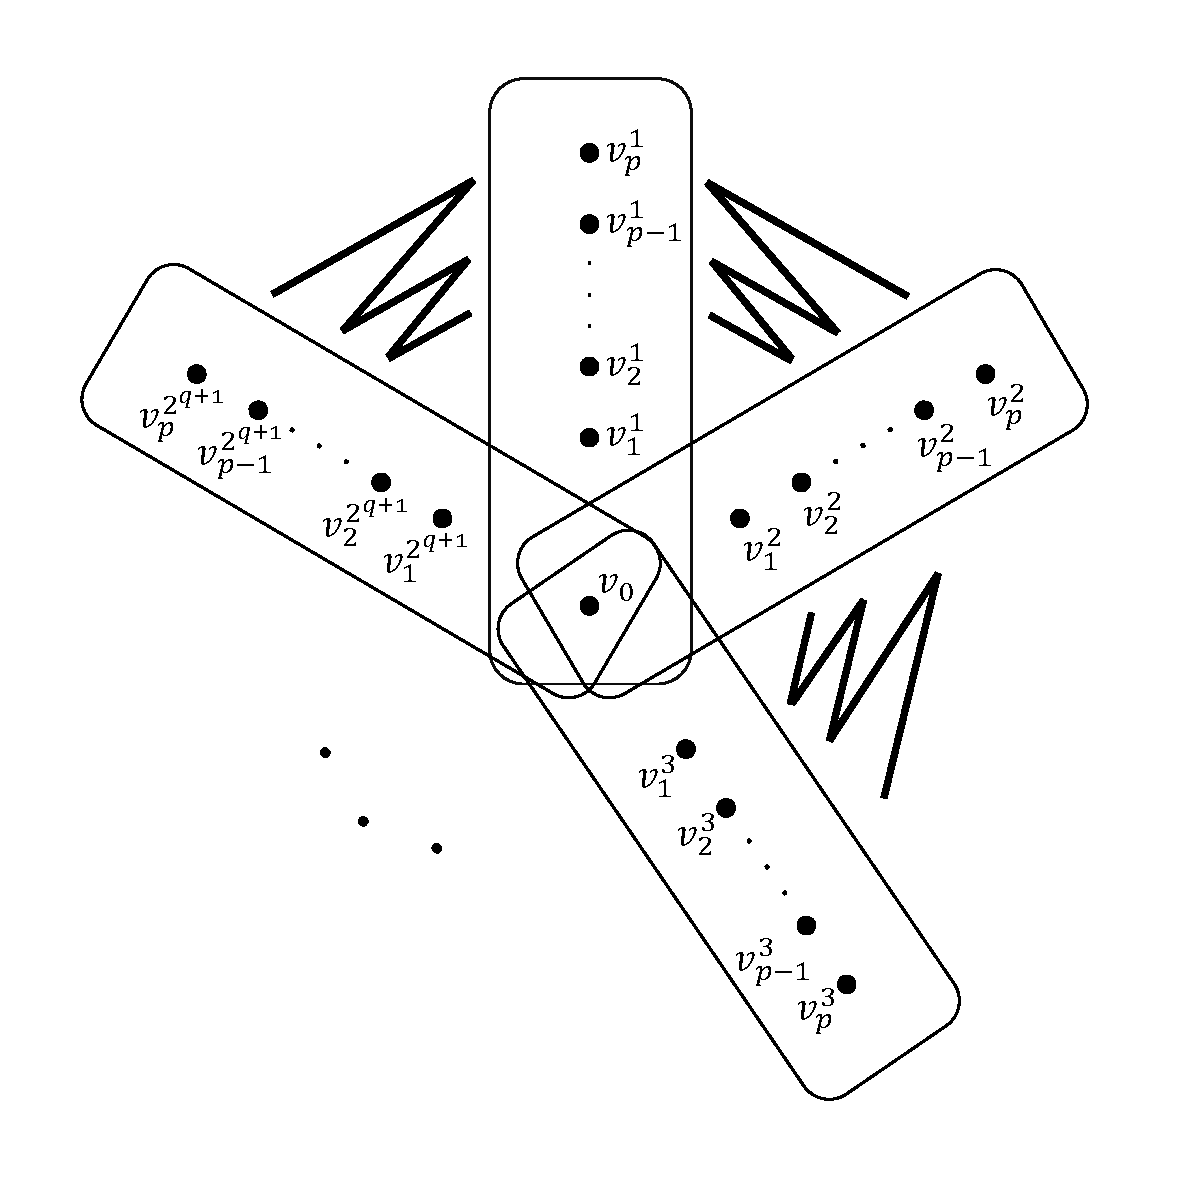
\includegraphics[width=0.7\textwidth]{figures/complete-graph-edges.pdf}
\caption{$K_{p2^{q+1}+1}$ գրաֆի գագաթները բաժանում ենք $2^{q+1}$ խմբերի այպես, որ կամայական երկու խմբի հատումը $v_0$ գագաթն է:}
\label{complete-graph}
\end{figure}

$K_{p2^{q+1}+1}$-ի $\phi$ կողային ներկումը կառուցենք օգտագործելով % compose !!!
տարբեր գրաֆների երեք ներկումներ:

\begin{enumerate}
    \item Մեզ հարկավոր է Թեորեմ \ref{tPetrosyan3n2}-ում նկարագրված $K_{p+1}$-ի $\alpha$ միջակայքային $\left(\frac{3}{2}(p+1)-2 \right)$-ներկումը: $K_{p+1}$-ի գագաթները նշանակենք հետևյալ կերպ. $V(K_{p+1}) = \{u_i : i=0, \ldots, p\}$: $\alpha$ ներկումը ունի մի կարևոր հատկություն, որ $\underline{S}(u_i, \alpha) = \lfloor \frac{i}{2} \rfloor + 1$ կամայական $i = 0,\ldots,p$ թվի համար:
    \item Այնուհետև, մեզ պետք է $K_{p,p}$-ի հատուկ տիպի ներկում, որը կնշանակենք $\beta$-ով: Դիցուք, $K_{p,p}$-ի գագաթներն են. $V(K_{p,p}) = \{x_i,y_i:i=1,\ldots,p\}$: $\beta$ ներկումը պետք է բավարարի հետևյալ պայմանին. կամայական $i=1,\ldots,p$ թվի համար $\underline{S}(x_i,\beta) = \underline{S}(y_i,\beta) = \left\lfloor \frac{i}{2} \right\rfloor + 1$: Այս պայմանին բավարարող $K_{p,p}$-ի ներկման գոյությունը հետևում է \cite{TepanyanPetrosyan} աշխատանքի Լեմմա 4-ից:
    \item Վերջապես, մեզ պետք է $K_{2^{q+1}+1}$ գրաֆի որևէ $\gamma$ ներկում $3\cdot2^q$ գույներով: Գրաֆի գագաթները նշանակենք $V(K_{2^{q+1}+1}) = \left\{w^j : j=0,\ldots, 2^{q+1} \right\}$: $\gamma$-ն պետք է բավարարի հետևյալ պայմանին. $def(K_{2^{q+1}+1},\gamma) = def(w^0, \gamma) = 2^q$: Այսպիսի հատկանիշներով ներկումներ նկարագրված են \cite{GiaroKubaleMalafiejski2001}-ի Թեորեմ 4.2-ում և \cite{PetrosyanMkhitaryan}-ի Թեորեմ 29-ում:
\end{enumerate}


$K_{p2^{q+1}+1}$ գրաֆի գագաթները նշանակենք հետևյալ կերպ (Նկ. \ref{complete-graph}). 
\begin{align*}
V\left(K_{p2^{q+1}+1}\right) = \{v_0\} \cup \left\{v_i^j : i=1,\ldots,p,\ j=1,\ldots,2^{q+1} \right\}.
\end{align*}

Կառուցենք նրա $\phi$ ներկումը հետևյալ կերպ.
\begin{align*}
\phi\left(v_{i_1}^j v_{i_2}^j\right) &= \alpha(u_{i_1}u_{i_2}) + p\left(\gamma(w^0w^j) - 1\right), & 0 \leq i_1 < i_2 \leq p, & & 1 \leq j \leq 2^{q+1}, \\
\phi\left(v_{i_1}^{j_1}v_{i_2}^{j_2}\right) &= \beta(x_{i_1}y_{i_2}) + p\left(\gamma(w^{j_1}w^{j_2}) - 1\right), & 1 \leq i_1, i_2 \leq p, & & 1 \leq j_1 < j_2 \leq 2^{q+1}: 
\end{align*} % !!! հայատառ վերջակետ

Վերևում բերված բանաձևերում $v_0^j$ սիմվոլները վերաբերվում են միևնույն $v_0$ գագաթին, % !!!!
կամայական $j=1,\ldots,2^{q+1}$ թվի համար: % !! թվի համար
Առաջին բանաձևը ներկում է այն կողերը, որոնց ծայրակետերը պատկանում են Նկ. \ref{complete-graph}-ում միևնույն խմբին, մինչդեռ երկրորդ բանաձևը ներկում է այն կողերը, որոնք միացնում են տարբեր խմբերին պատկանող գագաթները: Ցույց տանք, որ $v_i^j$, $i=1,\ldots,p$, $j=1,\ldots,2^{q+1}$, գագաթների սպեկտրները միջակայքեր են:
\begin{align*}
    S\left(v^j_i,\phi\right) &= \left[\underline{S}(u_i, \alpha) + p\left(\gamma(w^0w^j) - 1\right), \overline{S}(u_i, \alpha) + p\left(\gamma(w^0w^j) - 1\right)\right] \\
    &\cup \bigcup\limits_{j'\in [1, 2^{q+1}] \setminus \{j\}}{\left[\underline{S}(x_i, \beta) + p\left(\gamma(w^jw^{j'}) - 1\right), \overline{S}(x_i, \beta) + p\left(\gamma(w^jw^{j'}) - 1\right) \right]}.
\end{align*}
Ունենք, որ $\underline{S}(u_i, \alpha) = \underline{S}(x_i, \beta) = \lfloor \frac{i}{2} \rfloor + 1$ կամայական $i = 1,\ldots,p$ թվի համար: % Թվի համար
Ուստի վերը նշված արտահայտությունը դառնում է.
\begin{align*}
    S\left(v^j_i,\phi\right) &= \left[\left\lfloor \frac{i}{2} \right\rfloor + 1 + p\left(\gamma(w^0w^j) - 1\right), \left\lfloor \frac{i}{2} \right\rfloor + p + p\left(\gamma(w^0w^j) - 1\right)\right] \\
    &\cup \bigcup\limits_{j'\in [1, 2^{q+1}] \setminus \{j\}}{\left[\left\lfloor \frac{i}{2} \right\rfloor + 1 + p\left(\gamma(w^jw^{j'}) - 1\right), \left\lfloor \frac{i}{2} \right\rfloor + p + p\left(\gamma(w^jw^{j'}) - 1\right) \right]}\\
    &= \bigcup\limits_{j'\in [0, 2^{q+1}] \setminus \{j\}}{\left[\left\lfloor \frac{i}{2} \right\rfloor + 1 + p\left(\gamma(w^jw^{j'}) - 1\right), \left\lfloor \frac{i}{2} \right\rfloor + p + p\left(\gamma(w^jw^{j'}) - 1\right) \right]}\\
    &= \left[\left\lfloor \frac{i}{2} \right\rfloor + 1 + p\left(\underline{S}(w^j,\gamma) - 1\right), \left\lfloor \frac{i}{2} \right\rfloor + p + p\left(\overline{S}(w^j,\gamma) - 1\right) \right]:
\end{align*}
Վերջին հավասարությունը տեղի ունի, քանի որ $S\left(w^j, \gamma\right)$ սպեկտրը միջակայք է բոլոր $j=1,\ldots,2^{q+1}$ թվերի համար: Վերջապես, $v_0$-ի սպեկտրը և $\phi$ ներկման դեֆիցիտը $v_0$ գագաթում կլինեն.
\begin{align*}
    S\left(v_0,\phi\right) &= \bigcup\limits_{j'\in [1, 2^{q+1}]} {\left[ \underline{S}(u_0, \alpha) + p\left(\gamma(w^0w^{j'}) - 1\right), \overline{S}(u_0, \alpha) + p\left(\gamma(w^0w^{j'}) - 1\right) \right]}\\
    &= \bigcup\limits_{j'\in [1, 2^{q+1}]} {\left[ 1 + p\cdot\gamma(w^0w^{j'}) - p, p\cdot\gamma(w^0w^{j'}) \right]},\\
    def(v_0, \phi) &= \overline{S}(v_0, \phi) - \underline{S}(v_0, \phi)-d_{K_{2n+1}}(v_0) + 1\\
    &= p\cdot\overline{S}(w^0,\gamma) - (1 + p\cdot\underline{S}(w^0,\gamma) - p)-p\cdot2^{q+1} + 1\\
    &= p\left(\overline{S}(w^0,\gamma) - \underline{S}(w^0,\gamma)-d_{K_{2^{q+1}+1}}(w^0) + 1\right) = p\cdot def(w^0,\gamma) = p2^q = n:
\end{align*}

Դիցուք $w^{\underline{j}}$ և $w^{\overline{j}}$ $K_{2^{q+1}+1}$-ի այն գագաթներն են, որոնց համար $\underline{S}\left(w^{\underline{j}}, \gamma\right) = 1$ և $\overline{S}\left(w^{\overline{j}}, \gamma\right) = 3\cdot2^q$: Հեշտ է տեսնել, որ $\underline{S}\left(v^{\underline{j}}_{1},\phi\right) = 1$ և $\overline{S}\left(v^{\overline{j}}_{p},\phi\right) = \left\lfloor \frac{p}{2} \right\rfloor + p + p\left(3\cdot2^q - 1\right) = 3n + \frac{p-1}{2}$: Ուստի, $\phi$-ն $K_{2n+1}$-ի ճիշտ կողային ներկում է $3n + \frac{p-1}{2}$ գույներով, ընդ որում $def(K_{2n+1}, \phi) = def\left(v_0, \phi\right) = n$:
\end{proof}

Հայտնի է, որ եթե $G$-ն համասեռ մուլտիգրաֆ է, $G \in \mathfrak{N}$, իսկ $w(G) \leq t \leq W(G)$, ապա $G$-ն ունի միջակայքային $t$-ներկում: Հաջորդ թեորեմն ընդլայնում է այս արդյունքը դրական դեֆիցիտով մուլտիգրաֆների համար:

\begin{theorem}
\label{t3_middle_colors_def}
Դիցուք $\alpha_0$-ն $G$ համասեռ մուլտիգրաֆի ճիշտ ներկում է $t_0$ գույներով, իսկ $D \subseteq V(G)$ նրա գագաթների որևէ ենթաբազմություն է: Եթե կամայական $v \in V(G) \setminus D$ գագաթի համար $def(v,\alpha_0)=0$, ապա ցանկացած $t$ թվի համար, $\overline{S}(D,\alpha_0) - \underline{S}(D,\alpha_0) + 1 \leq t \leq t_0$, $G$-ն ունի $\alpha$ ճիշտ $t$-ներկում այնպես, որ $def(v,\alpha) = def(v,\alpha_0)$ կամայական $v\in V(G)$ գագաթի համար:
\end{theorem}
\begin{proof}[Ապացույց]
Դիցուք $a = \underline{S}(D,\alpha_0) - 1$ և $b = t_{0} - \overline{S}(D,\alpha_0)$: Փաստացի $[\underline{S}(D,\alpha_0),\overline{S}(D,\alpha_0)]$ միջակայքից դուրս ունենք $a+b$ գույներ, և պետք է ազատվել դրանցից $(t_0 - t)$-ից: Կառուցենք $G$-ի $\alpha$ ճիշտ կողային ներկումը՝ վերցնելով բոլոր կողերի գույները $\alpha_0$ ներկումից և ապա փոփոխելով դրանց մի մասը: Նախ կփորձենք ազատվել $\overline{S}(D,\alpha_0)$-ից մեծ գույներից, և եթե դա բավարար չլինի, կազատվենք $\underline{S}(D,\alpha_0)$-ից փոքր գույներից: 

Եթե $t_0 - t \leq b$, ապա կամայական $e\in E(G)$ կողի համար, որի համար $\alpha_0(e)\in \left[t + 1, t_0\right]$, նշանակենք $\alpha(e) = \alpha_0(e) - \Delta(G)$:

Եթե $t_0 - t > b$, ապա կամայական $e\in E(G)$ կողի համար, որի համար $\alpha_0(e)\in \left[\overline{S}(D, \alpha_0) + 1, t_0\right]$, նշանակենք $\alpha(e) = \alpha_0(e) - \Delta(G)$: Այնուհետև, կամայական $e\in E(G)$ կողի համար, որի համար $\alpha_0(e)\in \left[1, t_0 - t - b \right]$, նշանակենք $\alpha(e) = \alpha_0(e) + \Delta(G)$:
Երկու դեպքերում էլ $D$ բազմության գագաթների սպեկտրները չեն փոփոխվում, իսկ մյուս գագաթների սպեկտրները մնում են միջակայքեր: Եթե $\underline{S}(V(G), \alpha) > 1$, ապա վերջնական ներկումը ստանալու համար բոլոր կողերի գույներից հանում ենք  $\underline{S}(V(G), \alpha) - 1$:
\end{proof}


\begin{hide}
\begin{corollary}
\label{c3_complete_odd_colors}
Դիցուք $n=p2^q$, որտեղ $p$-ն կենտ է, իսկ $q \in \mathbb{Z}_+$: Կամայական $t$ թվի համար, $3n \leq t \leq 3n + \frac{p-1}{2}$, $K_{2n+1}$-ը ունի $\alpha$ ճիշտ ներկում $t$ գույներով այնպես, որ $def(K_{2n+1},\alpha)=n$:
\end{corollary}
\begin{proof}[Ապացույց] Բավական է վերցնել Թեորեմ \ref{t3_Wdef_wdef_difference}-ի ապացույցում նկարագրված $K_{2n+1}$-ի $\alpha_0$ ճիշտ կողային ներկումը $\left(3n + \frac{p-1}{2}\right)$ գույներով, վերցնել $D=\{v_0\}$, որտեղ $v_0\in V(K_{2n+1})$ և $def(v_0,\alpha_0)=def(K_{2n+1},\alpha_0)=n$, և հաշվի առնել, որ $\overline{S}(D,\alpha_0) - \underline{S}(D,\alpha_0) + 1=\overline{S}(v_0,\alpha_0) - \underline{S}(v_0,\alpha_0) + 1= def(v_0,\alpha_0)+d_{K_{2n+1}}(v_0) =n+2n =3n$:
\end{proof}
\end{hide}

\begin{hide}
\subsection{Որոշ գրաֆների դեֆիցիտի ճշգրիտ արժեքներ}
\end{hide}
\begin{frame}{$def(K_{2n+1} -e)$}
\begin{itemize}
    \item Բորովիցկա-Օլշեվսկան, Դրգաշ-Բուրչարդտը, Հալուշչակը առաջարկել էին հիպոթեզ.
\end{itemize}
\begin{hypothesis}[Բորովիցկա-Օլշեվսկա և այլոք, 2013]
Եթե $n\in \mathbb{N}$, ապա $def(K_{2n+1}-e)=n-1$:
\end{hypothesis}

\begin{theorem}[3.2.3]
Եթե $n\in \mathbb{N}$, ապա $def(K_{2n+1}-e)=n-1$, ընդ որում
$w_{def}(K_{2n+1}-e)=3n-1$:
\end{theorem}
\end{frame}

\begin{frame}{$K_{2n+1}-e$ գրաֆի մինիմալ դեֆիցիտով ներկումներ}{Օրինակ}

\begin{figure}
  \begin{center}
    % \tikzset{near start abs/.style={pos=1cm}}
    % \tikzset{near end abs/.style={pos=-1cm}}
  \begin{tikzpicture}[style=thick,scale=0.6, every node/.style={scale=0.6}]
    \coordinate (V3) at (-120:4.8cm);
    \coordinate (V2) at (-170:4.8cm);
    \coordinate (V1) at (140:4.8cm);
    \coordinate (V0) at (90:4.8cm);
    \coordinate (V4) at (40:4.8cm);
    \coordinate (V5) at (-10:4.8cm);
    \coordinate (V6) at (-60:4.8cm);
    
    \draw (V0) -- node [sloped,above,pos=0.4] {$1$} node [sloped,above,pos=0.6] {$1$} (V1);
    \draw (V0) -- node [sloped,above,pos=0.2] {$7$} node [sloped,above,pos=0.8] {$7$} (V2);
    \draw (V0) -- node [sloped,left,rotate=-90,pos=0.15] {$2$} node [sloped,left,rotate=-90,pos=0.85] {$2$} (V3);
    \draw (V0) -- node [sloped,above,pos=0.4] {$8$} node [sloped,above,pos=0.6] {$8$} (V4);
    \draw (V0) -- node [sloped,above,pos=0.2] {$3$} node [sloped,above,pos=0.8] {$3$} (V5);
    \draw (V0) -- node [sloped,left,rotate=90,pos=0.15] {$6$} node [sloped,left,rotate=90,pos=0.85] {$6$} (V6);
    
    \draw (V1) -- node [sloped,left,rotate=-90,pos=0.37] {$2$} node [sloped,left,rotate=-90,pos=0.63] {$2$} (V2);
    \draw (V1) -- node [sloped,left,rotate=90,pos=0.2] {$3$} node [sloped,left,rotate=90,pos=0.8] {$3$} (V3);
    \draw (V1) -- node [sloped,above,pos=0.2] {$4$} node [sloped,above,pos=0.8] {$4$} (V4);
    \draw (V1) -- node [sloped,above,pos=0.15] {$5$} node [sloped,above,pos=0.85] {$5$} (V5);
    % \draw (V1) -- node [sloped,left,rotate=-90] {$0$} (V6);
    
    \draw (V2) -- node [sloped,left,rotate=90,pos=0.37] {$6$} node [sloped,left,rotate=90,pos=0.63] {$6$} (V3);
    \draw (V2) -- node [sloped,above,pos=0.15] {$3$} node [sloped,above,pos=0.85] {$3$} (V4);
    \draw (V2) -- node [sloped,above,pos=0.15] {$4$} node [sloped,above,pos=0.85] {$4$} (V5);
    \draw (V2) -- node [sloped,above,pos=0.2] {$5$} node [sloped,above,pos=0.8] {$5$} (V6);
    
    \draw (V3) -- node [sloped,above,pos=0.15] {$5$} node [sloped,above,pos=0.85] {$5$} (V4);
    \draw (V3) -- node [sloped,above,pos=0.2] {$7$} node [sloped,above,pos=0.8] {$7$} (V5);
    \draw (V3) -- node [sloped,above,pos=0.37] {$4$} node [sloped,above,pos=0.63] {$4$} (V6);
    
    \draw (V4) -- node [sloped,right,rotate=90,pos=0.37] {$6$} node [sloped,right,rotate=90,pos=0.63] {$6$} (V5);
    \draw (V4) -- node [sloped,left,rotate=-90,pos=0.2] {$7$} node [sloped,left,rotate=-90,pos=0.8] {$7$} (V6);
    
    \draw (V5) -- node [sloped,right,rotate=-90,pos=0.37] {$8$} node [sloped,right,rotate=-90,pos=0.63] {$8$} (V6);
    
    \draw[fill=white,style=ultra thick] (V0) circle (3pt) node [above] {$v_0$};
    \draw[fill=black] (V1) circle (2pt) node [left] {$v_1$};
    \draw[fill=black] (V2) circle (2pt) node [left] {$v_2$};
    \draw[fill=black] (V3) circle (2pt) node [left] {$v_3$};
    \draw[fill=black] (V4) circle (2pt) node [right] {$v_4$};
    \draw[fill=black] (V5) circle (2pt) node [right] {$v_5$};
    \draw[fill=black] (V6) circle (2pt) node [right] {$v_6$};
  \end{tikzpicture}
  \end{center}
  \label{K7-minus-edge}
\end{figure}
$K_7-e$ գրաֆի $\beta$ ճիշտ կողային ներկումը $8$ գույներով, որտեղ $def( v_0,\beta)=def(K_7-e)=2$:
\end{frame}

\begin{frame}{$def(K_{1,m,n})$}
\begin{itemize}
\item (Ֆենգ, Հուանգ, 2007) $def\left(K_{1,1,n}\right)=0$, երբ $n$-ը զույգ է և $def\left(K_{1,1,n}\right)=1$, երբ $n$-ը կենտ է: 
\end{itemize}
\begin{theorem}[3.2.5]
Կամայական $m,n\in \mathbb{N}$ թվերի համար
\begin{center}
$def\left(K_{1,m,n}\right)=\left\{
\begin{tabular}{ll}
$0$, & երբ $(m+1,n+1)=1$,\\
$1$, & հակառակ դեպքում:\\
\end{tabular}%
\right.$
\end{center}
\end{theorem}
\end{frame}

\begin{hide}
\subsection{Միջակայքային ներկում չունեցող երկկողմանի գրաֆների ընտանիքներ}
\end{hide}
\begin{hide}
\begin{theorem}\cite{Giaro1999}
\label{t3_Giaro_14} Բոլոր երկկողմանի գրաֆները, որոնք ունեն առավելագույնը $14$ գագաթ միջակայքային ներկելի են:
\end{theorem}
\end{hide}

Փոքր առավելագույն աստիճանով երկկողմանի գրաֆների միջակայքային ներկելիության վերաբերյալ հայտնի են մի շարք արդյունքներ: Մասնավորապես, եթե $G$-ն երկկողմանի գրաֆ է, որի համար 
$\Delta(G)\leq 3$, ապա $G\in \mathfrak{N}$ և $w(G)\leq 4$\footnote{H.M. Hansen, Scheduling with minimum waiting periods, Master's Thesis, Odense University, Odense, Denmark, 1992 (դանիերեն).}: Երբ $\Delta(G) \leq 4$ և $G$-ն չունի $3$ աստիճան ունեցող գագաթ, ապա $G\in \mathfrak{N}$ և $w(G)=4$: Նաև հայտնի է, որ $G$ երկկողմանի գրաֆի համար միջակայքային $\Delta(G)$-ներկման գոյությունը կարելի է պարզել բազմանդամային ժամանակում, երբ $\Delta(G)\leq 4$, և $NP$-լրիվ է, եթե $\Delta(G)\geq 5$\footnote{K. Giaro, The complexity of consecutive $\Delta $-coloring of bipartite graphs: $4$ is easy, $5$ is hard, Ars Combin. 47, 1997, pp. 287-298.}: Միջակայքային ներկում չունեցող երկկողմանի գրաֆների օրինակներ կառուցվել են Միրումյանի, Սեվաստյանովի, Էրդյոշի, Հերցի, դե Վերրայի և Մալաֆիյսկու կողմից: Ջենսենը և Տոֆտը առաջարկել են հետևյալ խնդիրը.

\begin{hide}
\begin{theorem}
\label{t3_Hansen_Delta3}\cite{Hansen1992} Եթե $G$-ն երկկողմանի գրաֆ է, որի համար 
$\Delta(G)\leq 3$, ապա $G\in \mathfrak{N}$ և $w(G)\leq 4$.
\end{theorem}

\begin{theorem}
\label{t3_Giaro_Delta4_no3}\cite{Giaro1997}. Եթե $G$-ն երկկողմանի գրաֆ է, 
$\Delta(G)=4$ և այն չունի $3$ աստիճան ունեցող գագաթ, ապա $G\in
\mathfrak{N}$ և $w(G)=4$.
\end{theorem}

\begin{theorem}
\label{t3_Giaro_complexity}\cite{Giaro1997}. $G$ երկկողմանի գրաֆի համար միջակայքային $\Delta(G)$-ներկման գոյությունը կարելի է պարզել բազմանդամային ժամանակում, երբ $\Delta(G)\leq 4$, և $NP$-լրիվ է, եթե $\Delta(G)\geq 5$:
\end{theorem}

\begin{theorem}
\label{t3_GiaroKubaleMalafiejski_min3}\cite{GiaroKubaleMalafiejski1999} Եթե $G$-ն երկկողմանի գրաֆ է $(X,Y)$ կողմերով, իսկ $\min \{\vert X\vert, \vert Y\vert\}\leq 3$, ապա $G\in
\mathfrak{N}$:
\end{theorem}

\begin{figure}[h]
\begin{center}
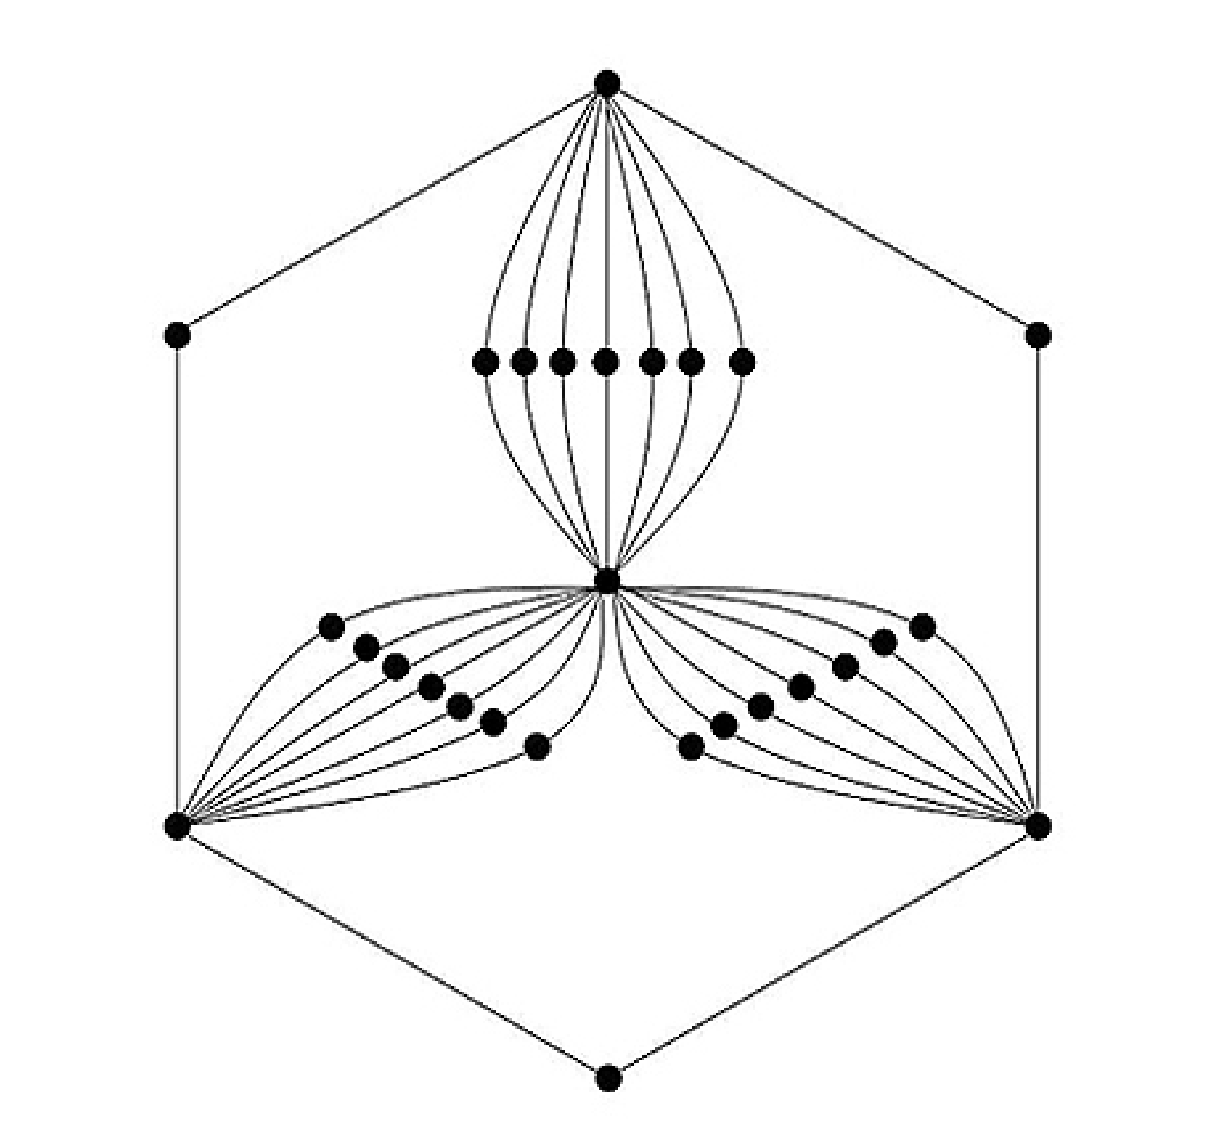
\includegraphics[width=25pc]{figures/sevastyanov.eps}\\
\caption{Սեվաստյանովի գրաֆը}\label{f3_sevastyanov}
\end{center}
\end{figure}
\end{hide}
\begin{problem}
Գոյություն ունի՞ երկկողմանի $G$ գրաֆ, որի համար $4\leq \Delta(G)\leq 12$ և
$G\notin \mathfrak{N}$:
\end{problem}

3.3 պարագրաֆում նկարագրվել են միջակայքային ներկում չունեցող երկկողմանի գրաֆների մի քանի ընտանիքներ՝ հիմնված Շեննոնի մուլտիգրաֆների, վերջավոր պրոյեկտիվ երկրաչափությունների, ծառերի և գրաֆների ենթատրոհումների վրա:

\begin{hide}
\begin{theorem}
\label{t3_Shannon} Եթե $r\geq 5$, ապա $\Delta_{r,s,t}\notin
\mathfrak{N}$:
\end{theorem}
\begin{proof}[Ապացույց]
Ենթադրենք հակառակը՝ $\Delta_{r,s,t}$ գրաֆը ունի  $\alpha$ միջակայքային $q$-ներկում ինչ որ $q$-ի համար, $q\geq r+s+t$:

Դիտարկենք $v$ գագաթը: Ենթադրենք $u$-ն և $w$-ն $v$-ին հարևան այն գագաթներն են, որոնց համար $\alpha(vu)=\underline{S}(v,\alpha)=p$ և
$\alpha(vw)=\overline{S}(v,\alpha)=p+r+s+t-1$: 
$\Delta_{r,s,t}$-ի կառուցման համաձայն $\Delta_{r,s,t}-v$ գրաֆում գոյություն ունի երկու երկարությամբ $P(u,w)$ շղթա, որը միացնում է $u$-ն  $w$-ին, որտեղ
\begin{center}
$P(u,w)=(u,uv^{\prime},v^{\prime},v^{\prime}w,w)$:
\end{center}

Քանի որ $d(u)=3$ և $d(v^{\prime})\leq s+t$, ունենք, որ

\begin{center}
$\alpha(uv^{\prime})\leq p+d(u)-1=p+2$, ուստի
\end{center}
\begin{center}
$\alpha(v^{\prime}w)\leq p+2+ d(v^{\prime})-1=p+1+s+t$:
\end{center}

Մյուս կողմից, քանի որ $d(w)=3$, ունենք, որ

\begin{center}
$p+r+s+t-1=\alpha(vw)=\overline{S}(v,\alpha)\leq p+1+s+t+d(w)-1=p+s+t+3$:
\end{center}
Այսպիսով, ստացանք, որ $r\leq 4$, ինչը հակասություն է:
\end{proof}

\begin{figure}[h]
\begin{center}
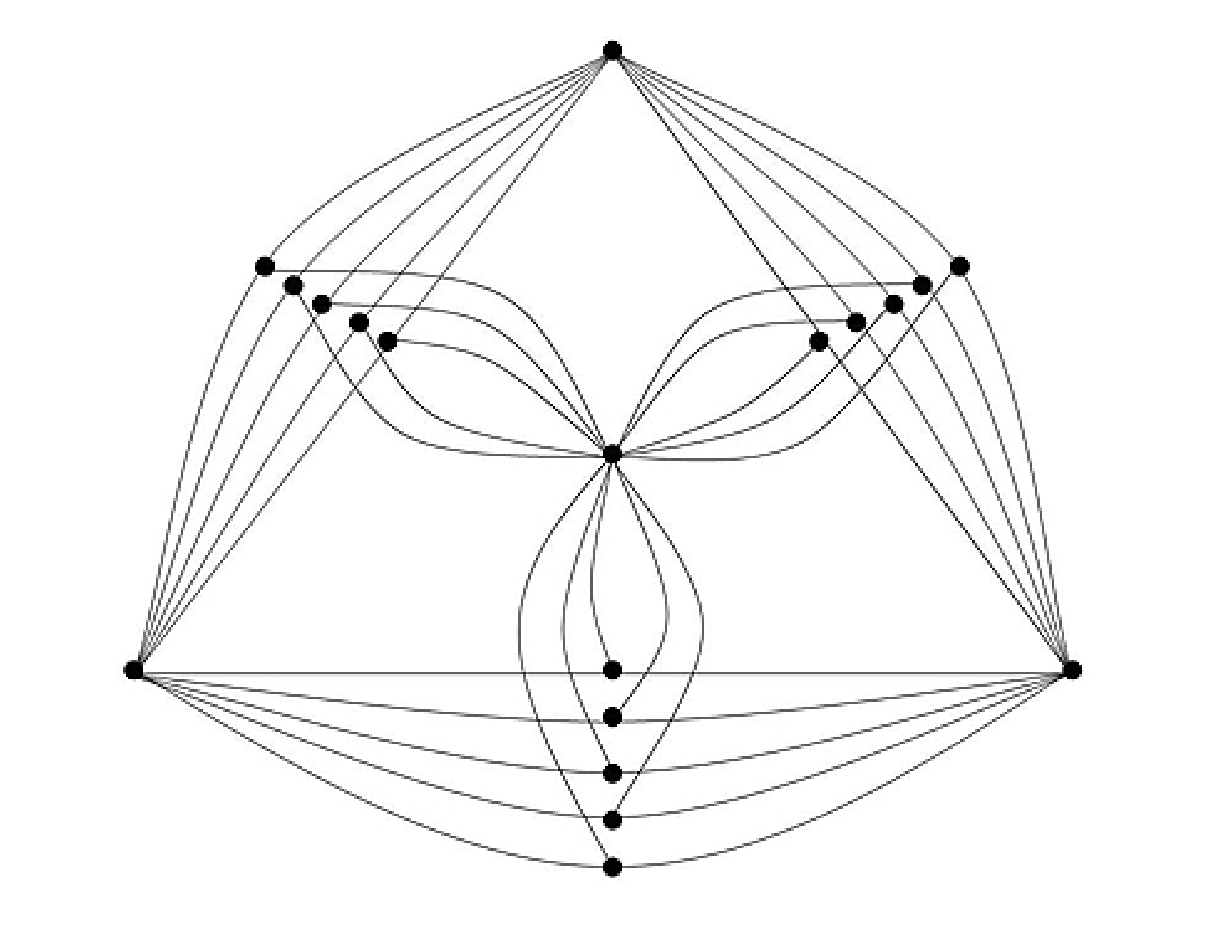
\includegraphics[width=30pc]{figures/shannon555.eps}\\
\caption{$\Delta_{5,5,5}$ գրաֆը}\label{f3_Shannon555}
\end{center}
\end{figure}

\begin{corollary}
\label{c3_Shannon} Ցանկացած $\Delta$ բնական թվի համար, $\Delta \geq 15$,
գոյություն ունի կապակցված երկկողմանի գրաֆ $G$, այնպես, որ $G\notin \mathfrak{N}$
և $\Delta(G)=\Delta$:
\end{corollary}

\begin{figure}[t]
\begin{center}
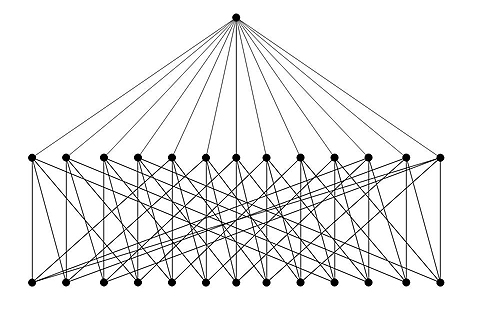
\includegraphics[width=30pc]{figures/erd13.jpg}\\
\caption{$Erd(1,1,1,1,1,1,1,1,1,1,1,1,1)$ գրաֆը:}\label{f3_Erd}
\end{center}
\end{figure}

\begin{theorem}
\label{t3_Erdos} Եթե $\underset{i=n+2}{\overset{n^{2}+n+1}{\sum
}}r_{i}> 2(n+1)$, ապա $Erd(r_{1},\ldots,r_{n^{2}+n+1})\notin
\mathfrak{N}$.
\end{theorem}
\begin{proof}[Ապացույց]
Ենթադրենք հակառակը.
$Erd(r_{1},\ldots,r_{n^{2}+n+1})$ գրաֆը ունի $\alpha$ միջակայքային $t$-ներկում
ինչ որ $t$-ի համար, $t\geq \underset{i=1}{\overset{n^{2}+n+1}{\sum
}}r_{i}$:

Դիտարկենք $u$ գագաթը: Դիցուք $v_{p}^{(l_{i_{0}})}$-ն և
$v_{q}^{(l_{j_{0}})}$-ն $u$-ին հարևան այն գագաթներն են, որոնց համար 
$\alpha\left(uv_{p}^{(l_{i_{0}})}\right)=\underline{S}(u,\alpha)=s$ և
$\alpha\left(uv_{q}^{(l_{j_{0}})}\right)=\overline{S}(u,\alpha)=s+\underset{i=1}{\overset{n^{2}+n+1}{\sum
}}r_{i}-1$:

Եթե $l_{i_{0}}=l_{j_{0}}$, ապա, ըստ 
$Erd(r_{1},\ldots,r_{n^{2}+n+1})$-ի կառուցման, գոյություն ունի $k_{0}$ այնպիսին, որ
$k_{0}v_{p}^{(l_{i_{0}})}$, $k_{0}v_{q}^{(l_{j_{0}})}\in
E(Erd(r_{1},\ldots,r_{n^{2}+n+1}))$: Եթե $l_{i_{0}}\neq l_{j_{0}}$,
ապա, ըստ $Erd(r_{1},\ldots,r_{n^{2}+n+1})$-ի կառուցման և
Հ2 հատկության, գոյություն ունի $k_{0}$ այնպիսին, որ
$k_{0}v_{p}^{(l_{i_{0}})}$, $k_{0}v_{q}^{(l_{j_{0}})}\in
E(Erd(r_{1},\ldots,r_{n^{2}+n+1}))$:

$Erd(r_{1},\ldots,r_{n^{2}+n+1})$-ի կառուցման համաձայն, ինչպես նաև Հ3 և Հ4 հատկություններից ելնելով ունենք, որ
$d\left(v_{p}^{(l_{i_{0}})}\right)=d\left(v_{q}^{(l_{j_{0}})}\right)=n+2$
և
\begin{center}
$\alpha\left(k_{0}v_{p}^{(l_{i_{0}})}\right)\leq
s+d\left(v_{p}^{(l_{i_{0}})}\right)-1=s+n+1$, ուստի
\end{center}
\begin{center}
$\alpha\left(k_{0}v_{q}^{(l_{j_{0}})}\right)\leq
s+n+1+d(k_{0})-1\leq s+n+\underset{i=1}{\overset{n+1}{\sum }}r_{i}$:
\end{center}

Հետևաբար,
\begin{center}
$s+\underset{i=1}{\overset{n^{2}+n+1}{\sum
}}r_{i}-1=\alpha\left(uv_{q}^{(l_{j_{0}})}\right)=\overline{S}(u,\alpha)\leq
s+n+\underset{i=1}{\overset{n+1}{\sum
}}r_{i}+d\left(v_{q}^{(l_{j_{0}})}\right)-1=s+2n+1+\underset{i=1}{\overset{n+1}{\sum
}}r_{i}$:
\end{center}

Այսպիսով ստանում ենք, որ $\underset{i=n+2}{\overset{n^{2}+n+1}{\sum }}r_{i}\leq
2(n+1)$, ինչը հակասություն է:
\end{proof}

\begin{corollary}
\label{c3_Erdos} Ցանկացած բնական $\Delta$-ի համար, $\Delta \geq 13$,
գոյություն ունի կապակցված երկկողմանի գրաֆ $G$, այնպես, որ $G\notin \mathfrak{N}$
և $\Delta(G)=\Delta$:
\end{corollary}

\begin{figure}[h]
\begin{center}
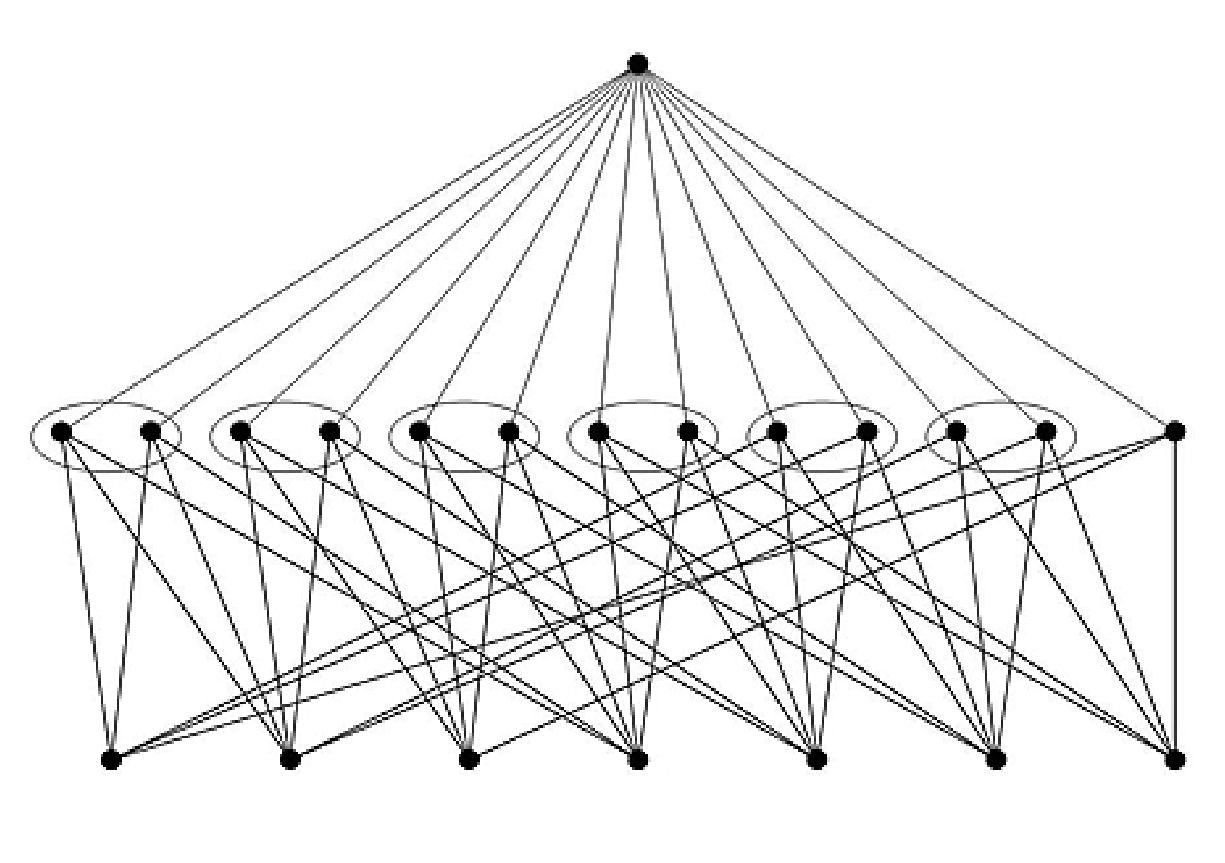
\includegraphics[width=30pc]{figures/erd6x2_1.eps}\\
\caption{$Erd(2,2,2,2,2,2,1)$ գրաֆը:}\label{f3_Erd6x2_1}
\end{center}
\end{figure}
\begin{theorem}
\label{t3_Kamalian_tree} Եթե $T$-ն ծառ է, ապա $T$-ն ունի միջակայքային $t$-ներկում այն և միայն այն դեպքում $\Delta(T)\leq t\leq M(T)$:
\end{theorem}

\begin{theorem}
\label{t3_tree} Եթե $T$-ն ծառ է, իսկ $\vert F(T)\vert >
M(T)+2$, ապա $\widetilde{T}\notin \mathfrak{N}$:
\end{theorem}
\begin{proof}[Ապացույց]
Ենթադրենք հակառակը, $\widetilde{T}$-ն ունի $\alpha$ միջակայքային $t$-ներկում ինչ որ $t$-ի համար, $t\geq \vert F(T)\vert$:

Դիտարկենք $u$ գագաթը: Դիցուք $v$-ն և $v^{\prime}$-ը $u$-ի հարևան այն երկու գագաթներն են, որոնց համար $\alpha(uv)=\underline{S}(u,\alpha)=s$ և
$\alpha(uv^{\prime})=\overline{S}(u,\alpha)=s+\vert F(T)\vert-1$: Քանտի որ $\widetilde{T}-u$ գրաֆը ծառ է, այնտեղ գոյություն ունի միակ շղթա
$P(v,v^{\prime})$, որը միացնում է $v$-ն և $v^{\prime}$-ը, որտեղ
\begin{center}
$P(v,v^{\prime})=(x_{1},e_{1},x_{2},\ldots,x_{i},e_{i},x_{i+1},\ldots,x_{k},e_{k},x_{k+1})$,
$x_{1}=v$, $x_{k+1}=v^{\prime}$:
\end{center}

Նկատենք, որ.
\begin{center}
$\alpha(x_{i}x_{i+1})\leq s+1+\underset{j=1}{\overset{i}{\sum
}}(d_{T}(x_{j})-1)$, երբ $1\leq i\leq k$:
\end{center}

Ստանում ենք, որ
\begin{center}
$\alpha(x_{k}x_{k+1})=\alpha(x_{k}v^{\prime})\leq
s+1+\underset{j=1}{\overset{k}{\sum
}}(d_{T}(x_{j})-1)=s+LP(v,v^{\prime})\leq s+M(T)$:
\end{center}

Այսպիսով,
\begin{center}
$s+\vert F(T)\vert -1=\overline{S}(u,\alpha)=\alpha(uv^{\prime})\leq
s+1+M(T)$, ուստի $\vert F(T)\vert\leq M(T)+2$,
\end{center}
ինչը հակասություն է:
\end{proof}

\begin{corollary}
\label{c3_tree} Եթե $T$-ն այնպիսի ծառ է, որի ցանկացած երկու կախված գագաթների միջև հեռավորությունը զույգ է և $\vert F(T)\vert >
M(T)+2$, ապա $\widetilde{T}$ երկկողմանի գրաֆը չունի միջակայքային ներկում:
\end{corollary}

\begin{figure}[h]
\begin{center}
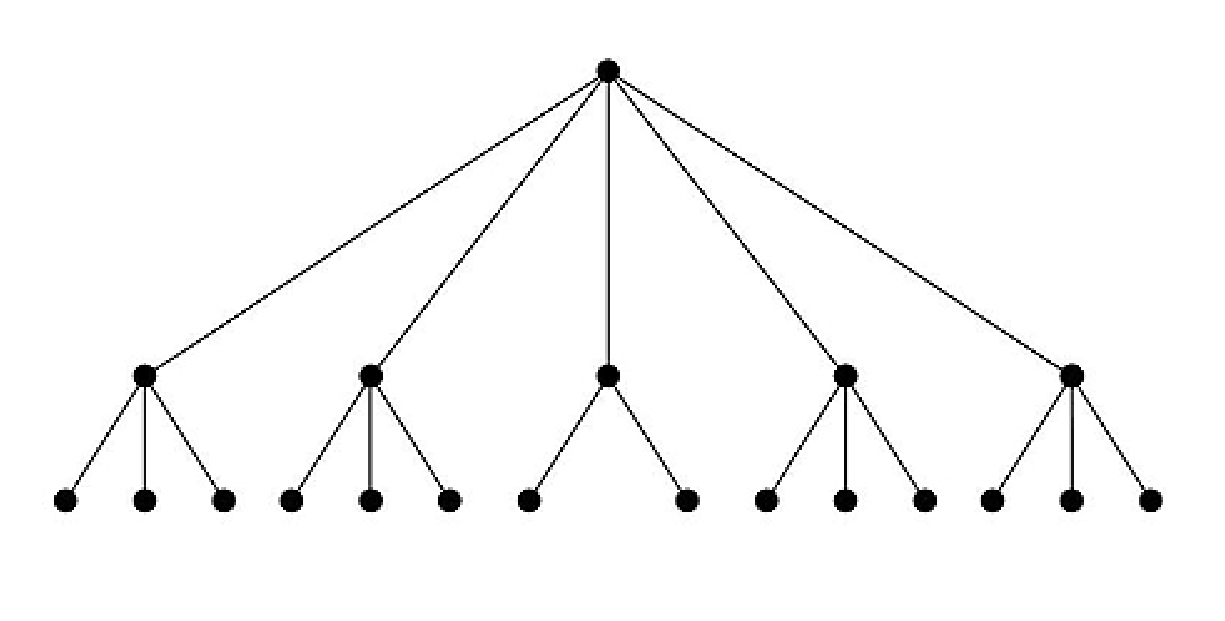
\includegraphics[width=20pc]{figures/tree.eps}\\
\caption{$T$ ծառը}\label{f3_tree}
\end{center}
\end{figure}
\end{hide}

Դիցուք $G$-ն գրաֆ է, $V(G)=\{v_{1},\ldots,v_{n}\}$: Սահմանենք 
$S(G)$ և $\widehat{G}$ գրաֆները հետևյալ կերպ.
\begin{align*}
V(S(G))&=\{v_{1},\ldots,v_{n}\}\cup \{w_{ij}:v_{i}v_{j}\in E(G)\},\\
E(S(G))&=\{v_{i}w_{ij},v_{j}w_{ij}:v_{i}v_{j}\in E(G)\},\\
V(\widehat{G})&=V(S(G))\cup \{u\}\text{, որտեղ } u\notin V(S(G)),\\
E(\widehat{G})&=E(S(G))\cup \{uw_{ij}:v_{i}v_{j}\in E(G)\}:
\end{align*}
$S(G)$ գրաֆը կոչվում է $G$-ի ենթատրոհում:

\begin{remark}
\label{r3_S(G)} Եթե $G$-ն երկկողմանի գրաֆ է և $G\in
\mathfrak{N}$, ապա $S(G)\in \mathfrak{N}$:
\end{remark}
\begin{proof}[Ապացույց]
Դիցուք $G$-ն երկկողմանի գրաֆ է $(X,Y)$ մասերով, որտեղ
$X=\{x_{1},\ldots,x_{r}\}$, $Y=\{y_{1},\ldots,y_{s}\}$, իսկ 
$\alpha$-ն $G$-ի միջակայքային $t$-ներկում է:

Սահմանենք $S(G)$-ի $\beta$ միջակայքային ներկումը հետևյալ կերպ.
\begin{center}
$\beta(x_{i}w_{ij})=\alpha(x_{i}y_{j})$ և
$\beta(y_{j}w_{ij})=\alpha(x_{i}y_{j})+1$, ցանկացած $x_{i}y_{j}\in
E(G)$-ի համար:
\end{center}

Հեշտ է համոզվել, որ $\beta$-ն $S(G)$-ի միջակայքային $(t+1)$-ներկում է:
\end{proof}

Հայտնի է\footnote{D. Hanson, C.O.M. Loten, B. Toft, On interval colorings of bi-regular bipartite graphs, Ars Combin. 50, 1998, pp. 23-32.}\textsuperscript{,}\footnote{Р.Р. Камалян, А.Н. Мирумян, Интервальные реберные раскраски двудольных графов одного класса, Доклады НАН РА, том 97, N 4, 1997, стр. 3-5.}, որ եթե $G$-ն համասեռ գրաֆ է, ապա $S(G)\in \mathfrak{N}$: Պետրոսյանը և Խաչատրյանը 2011-ին առաջարկել էին հիպոթեզ, համաձայն որի, եթե $G\in \mathfrak{N}$, ապա $S(G)\in \mathfrak{N}$: Այս հիպոթեզը հաստատվել է Պյատկինի կողմից\footnote{А.В. Пяткин, Об интервальной (1,1)-раскраске инциденторов интервально раскрашиваемых графов, Дискретн. анализ и исслед. опер. 22:2, 2015, стр. 63-72.}:
\begin{hide}
\begin{hypothesis}
Եթե $G\in \mathfrak{N}$, ապա $S(G)\in \mathfrak{N}$:
\end{hypothesis}
\end{hide}
\begin{theorem}
\label{t3_subdivision_paths} Եթե $G$-ն կապացված գրաֆ է, և
\begin{center}
$\vert E(G)\vert
> 1+ {\max\limits_{P\in \mathbf{P}}}{\sum\limits_{v\in
V(P)}}\ \left(d_{\widehat{G}}(v)-1\right)$,
\end{center}
որտեղ $\mathbf{P}$-ն $S(G)$-ում $w_{ij}$ գագաթները միացնող ամենակարճ շղթաների բազմությունն է, ապա $\widehat{G}\notin \mathfrak{N}$:
\end{theorem}
\begin{proof}[Ապացույց]
Ենթադրենք հակառակը, $\alpha$-ն $\widehat{G}$-ի միջակայքային 
$t$-ներկում է ինչ որ $t$-ի համար, $t\geq \vert E(G)\vert$:

Դիտարկենք $u$ գագաթը: Դիցուք $w$-ն և $w^{\prime}$-ը $u$-ին հարևան այն երկու գագաթներն են, որոնց համար $\alpha(uw)=\underline{S}(u,\alpha)=s$ և
$\alpha(uw^{\prime})=\overline{S}(u,\alpha)=s+\vert E(G)\vert-1$: Քանի որ $\widehat{G}-u=S(G)$ և $\widehat{G}-u$ գրաֆները կապակցված են, գոյություն ունի $w$-ն և $w^{\prime}$-ը միացնող կարճագույն $P(w,w^{\prime})$ շղթա $\widehat{G}-u$ գրաֆում, որտեղ
\begin{center}
$P(w,w^{\prime})=(x_{1},e_{1},x_{2},\ldots,x_{i},e_{i},x_{i+1},\ldots,x_{k},e_{k},x_{k+1})$,
$x_{1}=w$, $x_{k+1}=w^{\prime}$:
\end{center}

Նկատենք, որ
\begin{center}
$\alpha(x_{i}x_{i+1})\leq s+\underset{j=1}{\overset{i}{\sum
}}(d_{\widehat{G}}(x_{j})-1)$, երբ $1\leq i\leq k$
\end{center}
և
\begin{center}
$\alpha(x_{k+1}u)=\alpha(w^{\prime}u)\leq
s+\underset{j=1}{\overset{k+1}{\sum }}(d_{\widehat{G}}(x_{j})-1)$:
\end{center}

Հետևաբար,
\begin{center}
$s+\vert E(G)\vert -1=\overline{S}(u,\alpha)=\alpha(uw^{\prime})\leq
s+\underset{j=1}{\overset{k+1}{\sum }}(d_{\widehat{G}}(x_{j})-1)\leq
s+{\max\limits_{P\in \mathbf{P}}}{\sum\limits_{v\in V(P)}}\
\left(d_{\widehat{G}}(v)-1\right)$,
\end{center}
ուստի՝
\begin{center}
$\vert E(G)\vert \leq 1+{\max\limits_{P\in
\mathbf{P}}}{\sum\limits_{v\in V(P)}}\
\left(d_{\widehat{G}}(v)-1\right)$,
\end{center}
ինչը հակասություն է:
\end{proof}

\begin{hide}
\begin{corollary}
\label{c3_subdivision_complete} Եթե $n\geq 7$, ապա $\widehat{K}_{n}\notin
\mathfrak{N}$:
\end{corollary}
\begin{corollary}
\label{c3_subdivision_complete_bipartite} Եթե $mn-m-n>5$, ապա $\widehat{K}_{m,n}\notin \mathfrak{N}$:
\end{corollary}

\begin{figure}[h]
\begin{center}
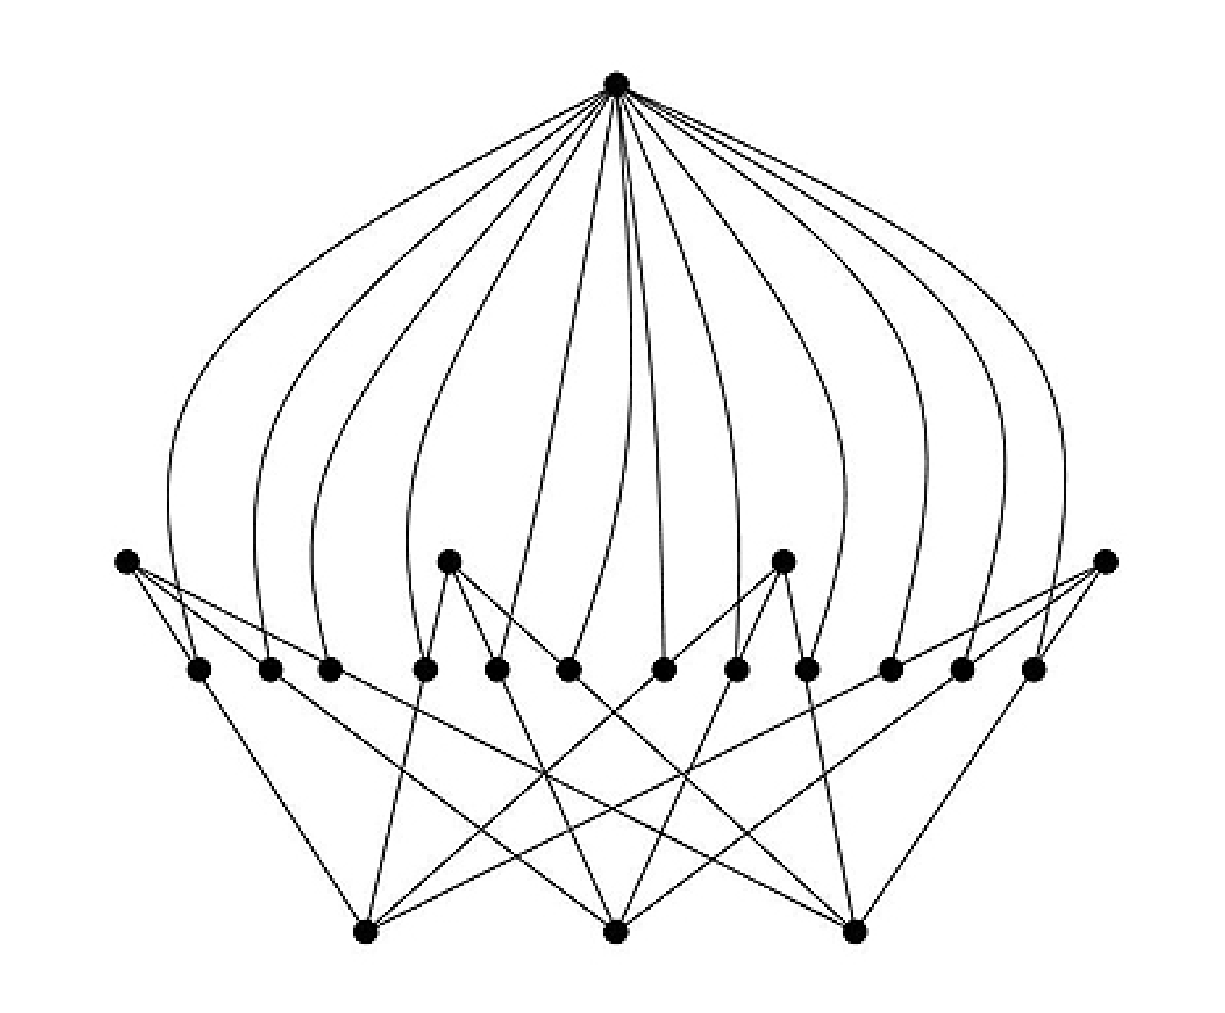
\includegraphics[width=25pc]{figures/subdivisionK34.eps}\\
\caption{$\widehat{K}_{3,4}$ գրաֆը:}\label{f3_subdivisionK34}
\end{center}
\end{figure}


\begin{theorem}
\label{t3_subdivision_K34} $\widehat{K}_{3,4}\notin \mathfrak{N}$:
\end{theorem}
\begin{proof}[Ապացույց]
Դիցուք
$V(\widehat{K}_{3,4})=\{u,v_{1},v_{2},v_{3},v_{4},v_{5},v_{6},v_{7}\}\cup
\{w_{ij}:1\leq i\leq 3, 4\leq j\leq 7\}$, իսկ
$E(\widehat{K}_{3,4})=\{v_{i}w_{ij},v_{j}w_{ij},uw_{ij}:1\leq i\leq
3, 4\leq j\leq 7\}$:

Ենթադրենք, որ $\alpha$-ն $\widehat{K}_{3,4}$-ի միջակայքային $t$-ներկում է ինչ որ $t$-ի համար, $t\geq 12$:

Դիտարկենք $u$ գագաթը: Դիցուք $w_{i_{0}j_{0}}$-ն և $w_{i_{1}j_{1}}$-ն
$u$-ին հարևան այն գագաթներն են, որոնց համար 
$\alpha(uw_{i_{0}j_{0}})=\underline{S}(u,\alpha)=s$ և
$\alpha(uw_{i_{1}j_{1}})=\overline{S}(u,\alpha)=s+11$: Դիտարկենք երկու դեպք:

Դեպք 1. $i_{0}=i_{1}$ կամ $j_{0}=j_{1}$:

Եթե $i_{0}=i_{1}$, ապա
$v_{i_{0}}w_{i_{0}j_{0}},v_{i_{0}}w_{i_{0}j_{1}}\in
E(\widehat{K}_{3,4})$: Հետևաբար,

\begin{center}
$\alpha(v_{i_{0}}w_{i_{0}j_{0}})\leq s+2$ և
$\alpha(v_{i_{0}}w_{i_{0}j_{1}})\leq s+5$:
\end{center}

Ուստի,
\begin{center}
$s+11=\overline{S}(u,\alpha)=\alpha(uw_{i_{0}j_{1}})\leq s+7$,
\end{center}
ինչը հնարավոր չէ:

Եթե $j_{0}=j_{1}$, ապա
$v_{j_{0}}w_{i_{0}j_{0}},v_{j_{0}}w_{i_{1}j_{0}}\in
E(\widehat{K}_{3,4})$: Հետևաբար,

\begin{center}
$\alpha(v_{j_{0}}w_{i_{0}j_{0}})\leq s+2$ և
$\alpha(v_{j_{0}}w_{i_{1}j_{0}})\leq s+4$:
\end{center}

Ուստի,
\begin{center}
$s+11=\overline{S}(u,\alpha)=\alpha(uw_{i_{1}j_{0}})\leq s+6$,
\end{center}
ինչը նույնպես հնարավոր չէ:

Դեպք 2. $i_{0}\neq i_{1}$ և $j_{0}\neq j_{1}$:

Այս դեպքում $v_{i_{0}}v_{j_{0}}$ և $v_{i_{1}}v_{j_{1}}$ կողերը անկախ են $K_{3,4}$-ում: Իսկ
$K_{3,4}$-ում ցանկացած երկու անկախ կող ընկած են 4 երկարությամբ ցիկլի վրա: Այսինքն, $\widehat{K}_{3,4}$-ում գոյություն ունի ցիկլ
$C=w_{i_{0}j_{0}}v_{j_{0}}w_{i_{1}j_{0}}v_{i_{1}}w_{i_{1}j_{1}}v_{j_{1}}w_{i_{0}j_{1}}v_{i_{0}}w_{i_{0}j_{0}}$, որը բաղկացած է $P$ և $Q$ շղթաներից, որտեղ
\begin{center}
$P=\left(w_{i_{0}j_{0}},v_{j_{0}}w_{i_{0}j_{0}},v_{j_{0}},v_{j_{0}}w_{i_{1}j_{0}},w_{i_{1}j_{0}},v_{i_{1}}w_{i_{1}j_{0}},v_{i_{1}},v_{i_{1}}w_{i_{1}j_{1}},w_{i_{1}j_{1}}\right)$
\end{center}
և
\begin{center}
$Q=\left(w_{i_{0}j_{0}},v_{i_{0}}w_{i_{0}j_{0}},v_{i_{0}},v_{i_{0}}w_{i_{0}j_{1}},w_{i_{0}j_{1}},v_{j_{1}}w_{i_{0}j_{1}},v_{j_{1}},v_{j_{1}}w_{i_{1}j_{1}},w_{i_{1}j_{1}}\right)$:
\end{center}

Եթե $\alpha(v_{j_{0}}w_{i_{0}j_{0}})\leq s+1$, ապա դիտարկելով $P$ շղթան ստանում ենք, որ $\alpha(v_{i_{1}}w_{i_{1}j_{1}})\leq s+8$ և
$\overline{S}(w_{i_{1}j_{1}},\alpha)\leq s+10$, ինչը հակասություն է:

Եթե $\alpha(v_{i_{0}}w_{i_{0}j_{0}})\leq s+1$, ապա դիտարկելով $Q$ շղթան ստանում ենք, որ $\alpha(v_{j_{1}}w_{i_{1}j_{1}})\leq s+8$ և
$\overline{S}(w_{i_{1}j_{1}},\alpha)\leq s+10$, ինչը ևս հակասություն է:

Ուստի, $\alpha(v_{j_{0}}w_{i_{0}j_{0}})\geq s+2$ և
$\alpha(v_{i_{0}}w_{i_{0}j_{0}})\geq s+2$, ինչը կրկին հակասություն է:
\end{proof}


\begin{figure}[h]
\begin{center}
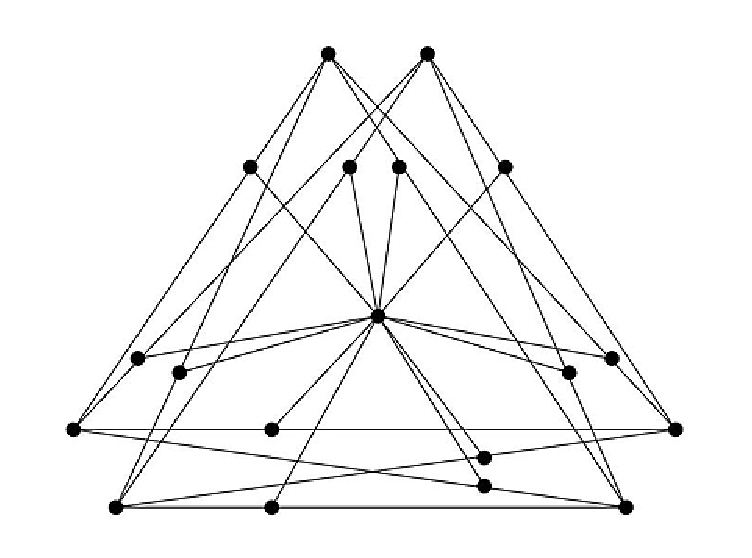
\includegraphics[width=25pc]{figures/K222.eps}\\
\caption{$\widehat{K}_{2,2,2}$ գրաֆը:}\label{f3_K222}
\end{center}
\end{figure}

\begin{theorem}
\label{t3_subdivision_K222} $\widehat{K}_{2,2,2}\notin \mathfrak{N}$:
\end{theorem}
\begin{proof}[Ապացույց]
Դիցուք
\begin{align*}
V(\widehat{K}_{2,2,2}) &=\{u,v_{1},v_{2},v_{3},v_{4},v_{5},v_{6}\}\cup
\{w_{ij}:1\leq i<j\leq 6,(i,j)\notin \{(1,2),(3,4),(5,6)\}\}\\
E(\widehat{K}_{2,2,2}) &=\{v_{i}w_{ij},v_{j}w_{ij},uw_{ij}:1\leq
i<j\leq 6,(i,j)\notin \{(1,2),(3,4),(5,6)\}\}
\end{align*}
Ենթադրենք $\alpha$-ն $\widehat{K}_{2,2,2}$-ի միջակայքային $t$-ներկում է ինչ որ $t$-ի համար, $t\geq 12$:

Դիտարենք $u$ գագաթը: Դիցուք, $w_{i_{0}j_{0}}$-ն և $w_{i_{1}j_{1}}$-ը $u$-ին հարևան այն երկու գագաթներն են, որոնց համար
$\alpha(uw_{i_{0}j_{0}})=\underline{S}(u,\alpha)=s$ և
$\alpha(uw_{i_{1}j_{1}})=\overline{S}(u,\alpha)=s+11$: $\widehat{K}_{2,2,2}$ գրաֆի սիմետրիայի համաձայն կարող ենք ենթադրել, որ 
$(i_{0},j_{0})=(1,6)$: Դիտարկենք երկու դեպք:

Դեպք 1. $v_{1}v_{6}$ և $v_{i_{1}}v_{j_{1}}$ հարևան են 
$K_{2,2,2}$-ում:

$\widehat{K}_{2,2,2}$ գրաֆի սիմետրիայից ելնելով բավական է դիտարկել այն դեպքը, երբ $(i_{1},j_{1})=(1,4)$ և $(i_{1},j_{1})=(1,5)$:

Եթե $\alpha(uw_{14})=s+11$ կամ $\alpha(uw_{15})=s+11$, ապա
$\alpha(v_{1}w_{16})\leq s+2$ և $\alpha(v_{1}w_{1j_{1}})\leq s+5$:
Ուստի, $\alpha(uw_{1j_{1}})\leq s+7$, ինչը հնարավոր չէ:

Դեպք 2. $v_{1}v_{6}$ և $v_{i_{1}}v_{j_{1}}$ անկախ են $K_{2,2,2}$-ում:

Հաշվի առնելով $\widehat{K}_{2,2,2}$ գրաֆի սիմետրիան, բավական է դիտարկել այն դեպքը, երբ $(i_{1},j_{1})=(4,5)$ և $(i_{1},j_{1})=(2,5)$:

Եթե $\alpha(uw_{45})=s+11$, ապա կամ $\alpha(v_{1}w_{16})=s+1$ կամ
$\alpha(v_{1}w_{16})=s+2$, և երկու դեպքերում էլ 
$C=w_{16}v_{1}w_{15}v_{5}w_{45}v_{4}w_{46}v_{6}w_{16}$ ցիկլի վրա գտնվող կողերի գույները որոշվում են միարժեքորեն:
Հետևաբար, $\alpha(v_{1}w_{14})\leq s+4$ և
$\alpha(v_{4}w_{14})\geq s+7$, ինչը հակասություն է:

Եթե $\alpha(uw_{25})=s+11$, ապա հաշվի առնելով 
$\widehat{K}_{2,2,2}$ գրաֆի սիմետրիան կարող ենք համարել, որ $\alpha(v_{1}w_{16})=s+1$:
Այս դեպքում 
$C=w_{16}v_{1}w_{15}v_{5}w_{25}v_{2}w_{26}v_{6}w_{16}$ ցիկլի վրա գտնվող բոլոր կողերի գույները որոշվում են միարժեքորեն: Հետևաբար, $\alpha(uw_{26})=s+6$: $\widehat{K}_{2,2,2}$ գրաֆի սիմետրիան հաշվի առնելով կարող ենք համարել, որ 
$\alpha(v_{1}w_{13})=s+2$ և $\alpha(v_{1}w_{14})=s+3$: Այժմ ցույց տանք, որ $\alpha(uw_{13})=s+1$: Քանի որ $S(u,\alpha)=[s,s+11]$, պետք է գոյություն ունենա կող $uw_{i^{\prime}j^{\prime}}$ որի համար
$\alpha\left(uw_{i^{\prime}j^{\prime}}\right)=s+1$: Քանի որ
$\alpha(v_{2}w_{25})=s+10$, ստանում ենք, որ $i^{\prime},j^{\prime}
\neq 2,5$: Եթե $\left(i^{\prime},j^{\prime}\right)\in
\{(1,4),(4,6)\}$, ապա $\alpha(uw_{24})=s+6$, ինչը հնարավոր չէ, քանի որ $\alpha(uw_{26})=s+6$: Մյուս կողմից, եթե 
$\left(i^{\prime},j^{\prime}\right)=(3,6)$, ապա հաշվի առնելով, որ
$\alpha(v_{6}w_{36})>s+2$, ստանում ենք, որ $\alpha(uw_{23})=s+6$, ինչը նույնպես հնարավոր չէ, քանի որ $\alpha(uw_{26})=s+6$: Ուստի, ստանում ենք, որ
$\left(i^{\prime},j^{\prime}\right)=(1,3)$: Հետևաբար,
$\alpha(v_{3}w_{13})=s+3$ և հաշվի առնելով, որ 
$\alpha(v_{2}w_{25})=s+10$, ստանում ենք, որ $\alpha(v_{3}w_{23})=s+6$: Սրանից հետևում է, որ $\alpha(v_{3}w_{35})\leq s+5$: Մյուս կողմից, քանի որ 
$\alpha(v_{5}w_{25})=s+9$, ունենք, որ $\alpha(v_{5}w_{35})\geq s+7$, ուտսի $\alpha(uw_{35})=s+6=\alpha(uw_{26})$, ինչը հակասություն է:
\end{proof}
\end{hide}

3.3 պարագրաֆում կառուցվել են երեք գրաֆներ, որոնք մասնակիորեն պատասխանում են Ջենսենի և Տոֆտի խնդրին. $\widehat{K}_{3,4} \notin \mathfrak{N}$, որտեղ $\Delta(\widehat{K}_{3,4})=12$, $|V(\widehat{K}_{3,4})|=20$, $\widehat{K}_{2,2,2} \notin \mathfrak{N}$, որտեղ $\Delta(\widehat{K}_{2,2,2})=12$, $|V(\widehat{K}_{2,2,2})|=19$, և  $\widehat{K}_{3,4}^{\prime} \notin \mathfrak{N}$, որտեղ $\widehat{K}_{3,4}^{\prime}$ գրաֆը ստացվում է $\widehat{K}_{3,4}$ գրաֆից՝ առավելագույն աստիճան ունեցող գագաթին կից կողերից մեկը հեռացնելով ($\Delta(\widehat{K}_{3,4}^{\prime})=11$, $|V(\widehat{K}_{3,4}^{\prime})|=20$):

\begin{hide}
\begin{theorem}
\label{t3_subdivision_K34_prime} $\widehat{K}_{3,4}^{\prime}\notin
\mathfrak{N}$:
\end{theorem}
\begin{proof}[Ապացույց]
Դիցուք $V(\widehat{K}_{3,4}^{\prime})= V(\widehat{K}_{3,4})$
և $E(\widehat{K}_{3,4}^{\prime})=E(\widehat{K}_{3,4})\setminus
\{uw_{l_{0}m_{0}}\}$:

Ենթադրենք $\alpha$-ն $\widehat{K}_{3,4}^{\prime}$-ի միջակայքային 
$t$-ներկում է ինչ որ $t$-ի համար, $t\geq 11$:

Դիտարկենք $u$ գագաթը: Դիցուք, $w_{i_{0}j_{0}}$-ն և $w_{i_{1}j_{1}}$-ը $u$-ին հարևան այն գագաթներն են, որոնց համար
$\alpha(uw_{i_{0}j_{0}})=\underline{S}(u,\alpha)=s$ և
$\alpha(uw_{i_{1}j_{1}})=\overline{S}(u,\alpha)=s+10$:

Դիցուք $S(w_{l_{0}m_{0}},\alpha)=\{c,c+1\}$: $\widehat{K}_{3,4}^{\prime}$ գրաֆին ավելացնենք 
$uw_{l_{0}m_{0}}$ կողը և ներկենք այն $c+2$ գույնով: Արդյունքում ստանում ենք $\widehat{K}_{3,4}$ գրաֆի ներկում $1,\ldots,t^{\prime}$ գույներով, 
$(t^{\prime}\geq t)$: Այս ներկումը նշանակենք $\beta$-ով: Նկատենք, որ ցանկացած $v$ գագաթի համար, $v\in V(\widehat{K}_{3,4})\setminus \{u\}$,
$S(v,\beta)$-ն ամբողջ թվերի միջակայք է, իսկ 
$S(u,\beta)=[s,s+10]\cup \{c+2\}$-ն ընդհանուր դեպքում մուլտիբազմություն է:

Թեորեմ \ref{t3_subdivision_K34}-ի Դեպք 1-ի ապացույցի նման կարելի է ցույց տալ, որ $i_{0}\neq i_{1}$ և
$j_{0}\neq j_{1}$: $v_{i_{0}}v_{j_{0}}$ և
$v_{i_{1}}v_{j_{1}}$ կողերը անկախ են $K_{3,4}$: Հաշվի առնելով $\widehat{K}_{3,4}$ գրաֆի սիմետրիան կարելի է համարել, որ
$(i_{0},j_{0})=(1,4)$ և $(i_{1},j_{1})=(3,7)$:

Դիտարկենք $v_{1}w_{14}$ կողը: Այն պետք է ներկված կլինի կամ
$\beta(v_{1}w_{14})=s+1$ գույնով կամ $\beta(v_{1}w_{14})=s+2$: Եթե
$\beta(v_{1}w_{14})=s+1$, ապա $C=w_{14}v_{1}w_{17}v_{7}w_{37}v_{3}w_{34}v_{4}w_{14}$ ցիկլի վրա գտնվող բոլոր կողերի գույները միարժեք որոշվում են: Արդյունքում ստացվում է, որ $\beta(uw_{17})=\beta(uw_{34})=s+5$: Հետևաբար $c+2$ ավելացված գույնը հավասար է $s+5$, ինչը սակայն հնարավոր չէ, քանի որ
$S(w_{17},\beta)=S(w_{34},\beta)=[s+4,s+6]$ և երկու դեպքում էլ $s+5$-ը $S(w_{17},\beta)$ և
$S(w_{34},\beta)$ բազմությունների միջին գույնն է:

Այժմ ենթադրենք, որ $\beta(v_{1}w_{14})=s+2$: Այդ դեպքում 
$C=w_{14}v_{1}w_{17}v_{7}w_{37}v_{3}w_{34}v_{4}w_{14}$ ցիկլի վրա գտնվող բոլոր կողերի գույները հայտնի են: $\widehat{K}_{3,4}$ գրաֆի սիմետրիայի համաձայն կարող ենք համարել, որ $\beta(v_{1}w_{15})=s+3$ և $\beta(v_{1}w_{16})=s+4$:
Քանի որ $\beta(v_{7}w_{27})=s+8$, ունենք, որ $\underline{S}(v_{2},\beta)\geq
s+3$. Մյուս կողմից, քանի որ $\beta(v_{4}w_{24})=s+2$, ստանում ենք, որ
$\underline{S}(v_{2},\beta)\leq s+4$: Քննարկենք երկու դեպք:

Դեպք 1. $\underline{S}(v_{2},\beta)= s+3$:

Ապացուցենք, որ $\beta(uw_{36})= s+9$: Քանի որ
$S(u,\alpha)=[s,s+10]$, պետք է գոյություն ունենա 
$uw_{i^{\prime}j^{\prime}}$ կող, որի համար
$\beta\left(uw_{i^{\prime}j^{\prime}}\right)=s+9$: Քանի որ $\overline{S}(v_{1},\beta)= s+5$ և $\overline{S}(v_{2},\beta)= s+6$, ունենք, որ
$i^{\prime}\neq 1,2$, ուստի $i^{\prime}=3$: Քանի որ
$\beta(v_{3}w_{37})= s+8$ և $i^{\prime}=3$, ստանում ենք, որ
$\beta(v_{3}w_{3j^{\prime}})= s+7$,
$\beta(v_{j^{\prime}}w_{3j^{\prime}})= s+8$ և
$\beta(v_{1}w_{1j^{\prime}})\geq s+4$: Այսպիսով, ունենք, որ $j^{\prime}=6$
և $\left(i^{\prime},j^{\prime}\right)=(3,6)$: Հետևաբար, 
$\beta(v_{6}w_{26})= s+7$: Քանի որ $\beta(v_{7}w_{27})= s+8$, ունենք, որ
$\beta(v_{2}w_{26})\leq s+5$, ուստի $\beta(uw_{26})= s+6$: Մյուս կողմից ունենք, որ $\beta(uw_{17})= s+6$, ինչը հնարավոր չէ,
քանի որ $S(w_{17},\beta)=S(w_{26},\beta)=[s+5,s+7]$ և երկու դեպքերում էլ $s+6$ գույնը ($c+2$ ավելացված գույնը) 
$S(w_{17},\beta)$ և $S(w_{26},\beta)$ բազմություների միջին գույնն է:

Դեպք 2. $\underline{S}(v_{2},\beta)= s+4$:

Այս դեպքում $\beta(uw_{24})=s+3$ և $\beta(v_{2}w_{24})= s+4$:
Հետևաբար, $\beta(v_{2}w_{25})\geq s+5$: Այժմ ցույց տանք, որ
$\beta(uw_{15})= s+1$: Քանի որ $S(u,\alpha)=[s,s+10]$, պետք է գոյություն ունենա կող $uw_{i^{\prime}j^{\prime}}$, որի համար
$\beta\left(uw_{i^{\prime}j^{\prime}}\right)=s+1$: Քանի նոր $\underline{S}(v_{2},\beta)= s+4$ և $\underline{S}(v_{3},\beta)= s+5$, ունենք, որ
$i^{\prime}\neq 2,3$, ուստի $i^{\prime}=1$: Քանի որ
$\beta(v_{1}w_{16})=s+4$ և $i^{\prime}=1$, ստանում ենք, որ
$j^{\prime}=5$ և $\left(i^{\prime},j^{\prime}\right)=(1,5)$: Սրանից հետևում է, որ $\beta(v_{5}w_{15})= s+2$: Քանի որ
$\beta(v_{3}w_{35})\geq s+6$, ունենք, որ $\beta(v_{5}w_{35})= s+4$ և
$\beta(v_{5}w_{25})= s+3$: Հետևաբար, $\beta(uw_{25})= s+4$:
Մյուս կողմից, $\beta(uw_{34})= s+4$, ինչը հնարավոր չէ, քանի որ $S(w_{34},\beta)=S(w_{25},\beta)=[s+3,s+5]$ և
երկու դեպքերում էլ $s+4$ գույնը ($c+2$ ավելացված գույնը) $S(w_{34},\beta)$ և $S(w_{25},\beta)$ բազմությունների միջին գույնն է:
\end{proof}
\end{hide}

\begin{hide}
\subsection {Փոքրաթիվ գագաթներով երկկողմանի գրաֆների միջակայքային ներկումներ}
\end{hide}
\begin{frame}[shrink]{Միջակայքային ներկում չունեցող երկկողմանի գրաֆներ}

\begin{itemize}
\item (Գիառո, 1999) Բոլոր երկկողմանի գրաֆները, որոնք ունեն առավելագույնը $14$ գագաթ, միջակայքային ներկելի են:
\end{itemize}

\begin{theorem}[3.4.4]
Բոլոր երկկողմանի գրաֆները, որոնք ունեն $15$ կամ $16$ գագաթ, միջակայքային ներկելի են:
\end{theorem}
\begin{table}[t]
\begin{center}
\begin{tabular}{|c|r|r|}
\hline
$|V(G)|$ & Գրաֆների քանակ & Ներկված գրաֆների քանակ \\
\hline
14 & 33 985 853 &  \\
\hline
15 & 611 846 940 & 288 643 868 \\
\hline
16 & 14 864 650 924 & 12 322 367 816 \\
\hline
17 & 488 222 721 992 &  \\
\hline
\end{tabular}
\end{center}
\end{table}

\end{frame}


\begin{hide}
\subsection{Միջակայքային ներկում չունեցող երկկողմանի մուլտիգրաֆներ}\
\end{hide}
\begin{frame}{Միջակայքային ներկում չունեցող երկկողմանի մուլտիգրաֆներ}
\begin{theorem}[3.5.3]
Եթե $G$-ն կապակցված երկկողմանի մուլտիգրաֆ է, ընդ որում $\vert V(G)\vert\leq 4$, ապա $G\in \mathfrak{N}$: Իսկ ցանկացած $n \geq 5$ թվի համար գոյություն ունի $G$ կապակցված երկկողմանի մուլտիգրաֆ, որի համար $G\notin \mathfrak{N}$ և $|V(G)|=n$:
\end{theorem}

\begin{figure}[h]
\begin{center}
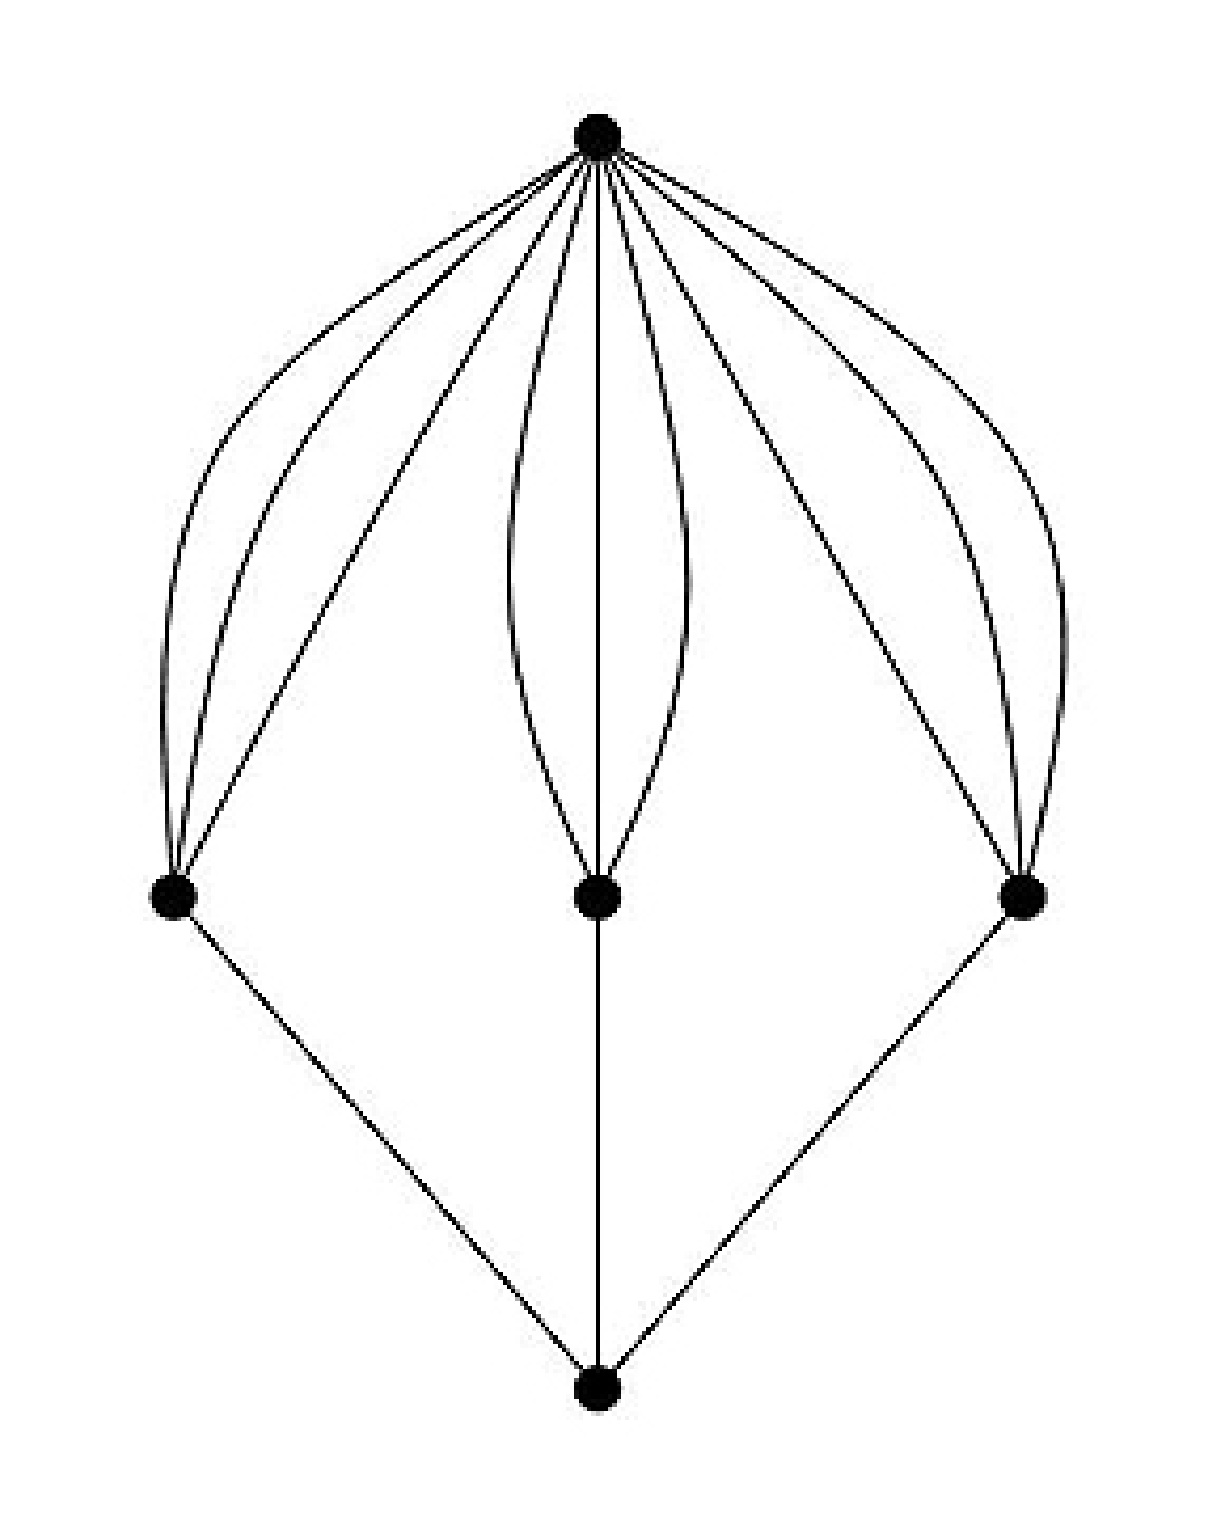
\includegraphics[width=0.25\textwidth]{figures/parachute.eps}
\end{center}
\end{figure}
\end{frame}

\begin{frame}{Միջակայքային ներկում չունեցող երկկողմանի մուլտիգրաֆներ}


\begin{figure}[h]
\begin{center}
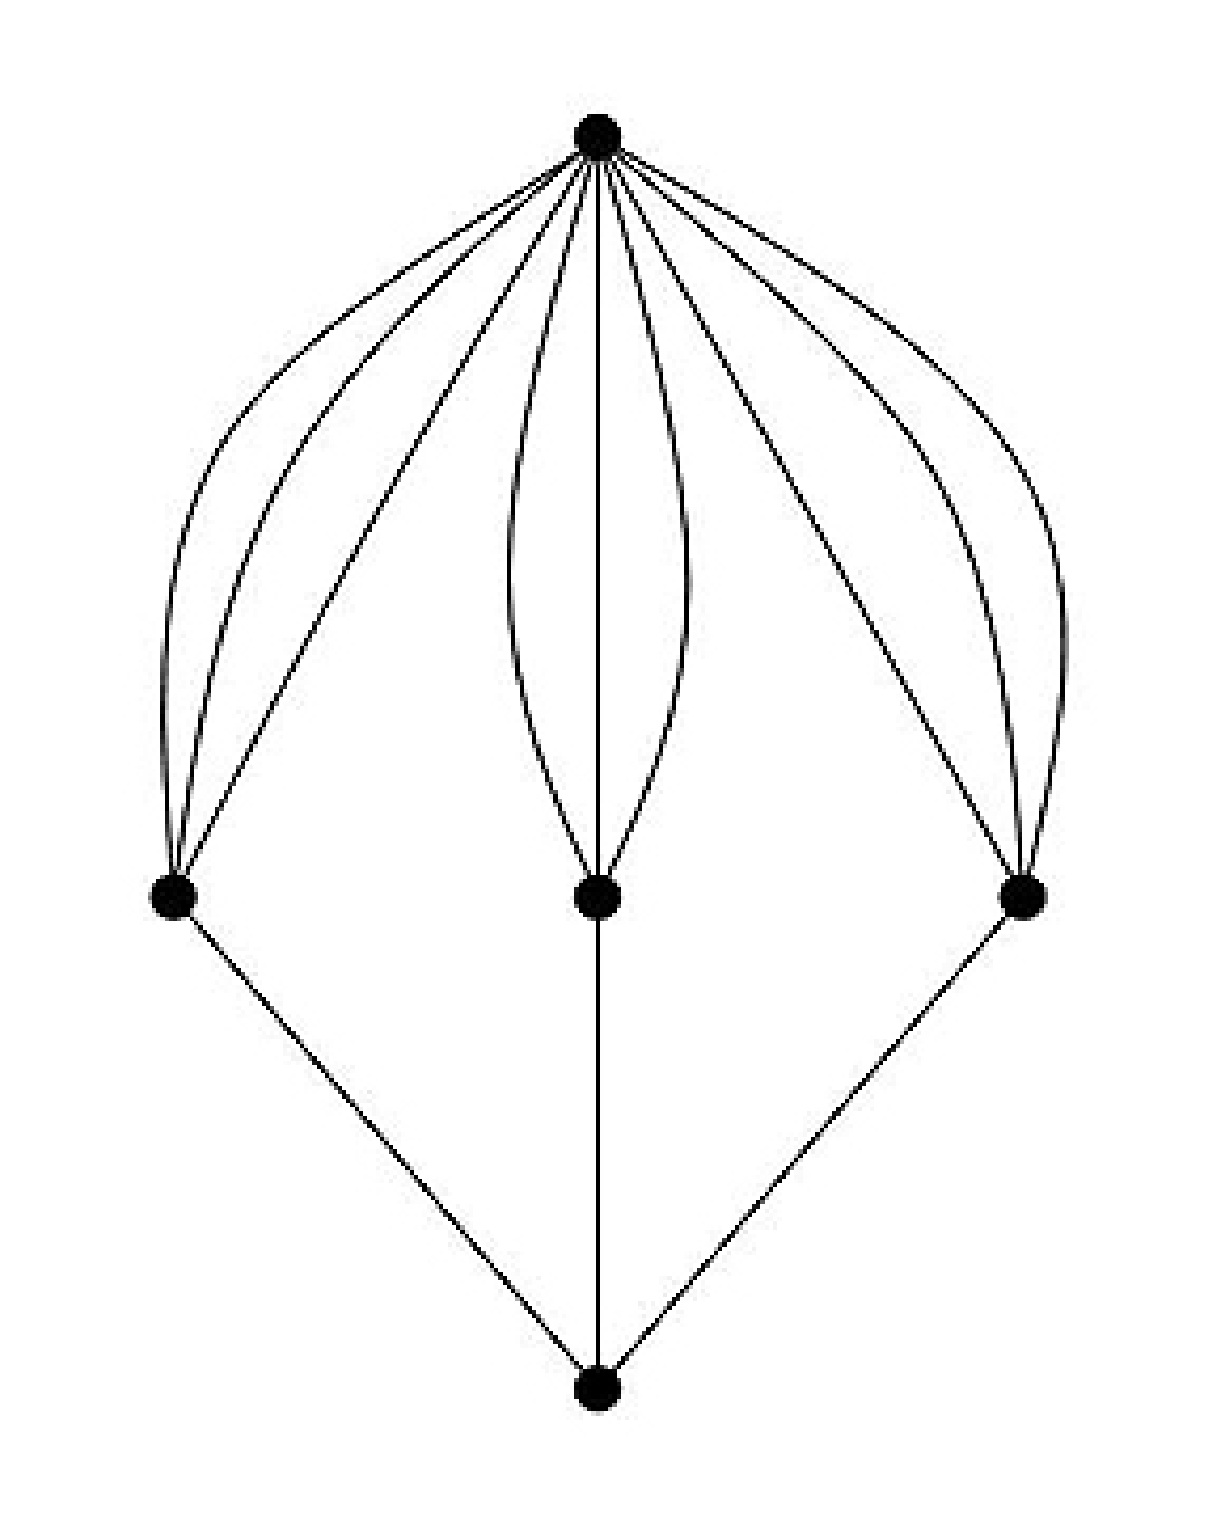
\includegraphics[width=0.25\textwidth]{figures/parachute.eps}
\end{center}
\end{figure}

\begin{theorem}[3.5.4]
Եթե $G$-ն երկկողմանի մուլտիգրաֆ է, որի համար
$\Delta(G)\leq 3$, ապա $G\in \mathfrak{N}$ և $w(G)\leq 4$: Իսկ ցանկացած $\Delta \geq 9$ թվի համար գոյություն ունի $G$ կապակցված երկկողմանի մուլտիգրաֆ, որի համար $G\notin \mathfrak{N}$ և $\Delta(G)=\Delta$:
\end{theorem}

\end{frame}


\section*{Հիմնական արդյունքներն ու հետևությունները}\
Կարգացուցակների կառուցման բազմաթիվ խնդիրներ բերվում են տարաբնույթ պայմաններով գրաֆների կողային ներկումների խնդիրների ուսումնասիրությանը: Մասնավորապես, «պատուհան» չունեցող դասացուցակների գոյության և կառուցման խնդիրները մոդելավորվում են գրաֆների (մուլտիգրաֆների) միջակայքային կողային ներկումների միջոցով: Այս աշխատանքը նվիրված է այդպիսի ներկումների և նրանց տարբեր բնույթի ընդհանրացումների հետազոտմանը: 

$G$ մուլտիգրաֆի գագաթների և կողերի բազմությունը նշանակենք, համապատասխանաբար, $V(G)$-ով և $E(G)$-ով: $\Delta(G)$-ով նշանակենք գրաֆի առավելագույն աստիճանը: $\alpha : E(G) \rightarrow \mathbb{N}$ ֆունկցիան կոչվում է $G$ մուլտիգրաֆի ճիշտ կողային ներկում, եթե ցանկացած $v\in V(G)$ գագաթին կից կողերը ներկված են զույգ առ զույգ տարբեր գույներով: Եթե $\alpha$-ն ճիշտ կողային ներկում է, $S(v,\alpha)$-ով նշանակում ենք $v$ գագաթին կից կողերի գույների բազմությունը, իսկ $\underline{S}(v, \alpha)$-ով և $\overline{S}(v, \alpha)$-ով՝ այդ բազմության փոքրագույն և մեծագույն գույները:
    
$\alpha : E(G) \rightarrow \{1,\ldots,t\}$ ճիշտ կողային ներկումը կոչվում է $G$ մուլտիգրաֆի միջակայքային $t$-ներկում, եթե կամայական $i$ թվի համար, $i=1,\ldots,t$, գոյություն ունի $e$ կող, որ $\alpha(e)=i$, իսկ կամայական $v \in V(G)$ գագաթի համար $S(v,\alpha)$ բազմությունը հանդիսանում է բնական թվերի միջակայք:

$\mathfrak{N}_t$-ով նշանակենք այն մուլտիգրաֆների բազմությունը, որոնք ունեն միջակայքային կողային $t$-ներկում, իսկ $\mathfrak{N}$-ով՝ $\mathfrak{N} = \bigcup\limits_{t \geq 1}{\mathfrak{N}_t}$, բոլոր միջակայքային կողային ներկելի գրաֆների բազմությունը: Եթե $G \in \mathfrak{N}$, $w(G)$-ով և $W(G)$-ով նշանակենք $t$-ի փոքրագույն և մեծագույն արժեքները, որոնց դեպքում $G$-ն ունի միջակայքային կողային $t$-ներկում:

Քանի որ ոչ բոլոր մուլտիգրաֆները ունեն միջակայքային ներկումներ, դիտարկվում են միջակայքային կողային ներկումների ընդհանրացումներ: Կամայական $G$ մուլտիգրաֆի $\alpha$ կողային ներկման համար սահմանվում է այդ ներկման դեֆիցիտը՝ $def(G, \alpha) = \sum\limits_{v\in V(G)}{\left(\overline{S}(v,\alpha)-\underline{S}(v,\alpha) - |S(v,\alpha)|+1\right)}$: $G$ մուլտիգրաֆի դեֆիցիտը՝ $def(G)$-ն, $G$-ի բոլոր ճիշտ կողային ներկումների դեֆիցիտներից նվազագույնն է: $w_{def}(G)$-ով և $W_{def}(G)$-ով նշանակում ենք $t$-ի փոքրագույն և մեծագույն արժեքները, որոնց համար $G$-ն ունի $t$ գույներով և $def(G)$ դեֆիցիտով ճիշտ կողային ներկում: 

$G$ և $H$ գրաֆների $G\square H$ դեկարտյան արտադրյալը սահմանվում է հետևյալ կերպ.
\begin{align*}
V(G \square H) &= V(G) \times V(H) \\
E(G \square H) &= \left\{(u_1,v_1)(u_2,v_2) : (u_1=u_2 \text{ և } v_1v_2 \in E(H)) \text{ կամ } (v_1=v_2 \text{ և } u_1u_2 \in E(G) \right\}
\end{align*}

Այս աշխատանքում դիտարկվել են մուլտիգրաֆների տարբեր դասերի՝ $\mathfrak{N}$ դասին պատկանելու խնդիրներ, այդ դասին պատկանող մուլտիգրաֆների համար՝ $w(G)$ և $W(G)$ պարամետրերի գնահատման և ճշգրիտ արժեքների որոշման խնդիրներ, միջակայքային ներկումներում մասնակցող գույների հնարավոր քանակի որոշման խնդիրներ, գրաֆների տարբեր գործողությունների նկատմամբ միջակայքային ներկելիության կայունության խնդիրներ, ինչպես նաև ուսումնասիրվել են միջակայքային ներկում չունեցող գրաֆների դեֆիցիտը և $w_{def}(G)$ ու $W_{def}(G)$ պարամետրերը:

Աշխատանքում ստացվել են հետևյալ արդյունքները:

1) Միջակայքային ներկումներ ունեցող գրաֆների և մուլտիգրաֆների $w(G)$ և $W(G)$ պարամետրերի, ինչպես նաև միջակայքային ներկում չունեցող գրաֆների $w_{def}(G)$ և $W_{def}(G)$ պարամետրերի համար տրվել են հասանելի գնահատականներ,

2) $K_{2n}$ լրիվ գրաֆների միջակայքային կողային ներկումների և այդ գրաֆների հատուկ տիպի ֆակտորիզացիաների համարժեքության հիման վրա ստացվել են  $W(K_{2n})$ պարամետրի նոր ստորին և վերին գնահատականներ, գտնվել են այդ պարամետրի ճշգրիտ արժեքները $n \leq 12$ արժեքների համար,

3) Ստացվել են լրիվ բազմակողմանի գրաֆների, արտաքին հարթ գրաֆների, ցանցերի, գլանների, տոռերի և Հեմինգի գրաֆների միջակայքային կողային ներկումների գոյության վերաբերյալ արդյունքներ, $w(G)$ և $W(G)$ պարամետրերի գնահատականներ, որոշ դեպքերում՝ նաև ճշգրիտ արժեքներ,

4) Ցույց է տրվել գրաֆների միջակայքային ներկելիության կապը այդ գրաֆների մասնակցությամբ դեկարտյան արտադրյալների միջակայքային ներկելիություն հետ, էապես ուժեղացվել են համասեռ գրաֆների մասնակցությամբ դեկարտյան արտադրյալների համար $W(G \square H)$ պարամետրի հայտնի գնահատականները, ապացուցվել է երկկողմանի գրաֆների մասնակցությամբ դեկարտյան արտադրյալների մի շարք դասերի միջակայքային ներկելիությունը,

5) Գտնվել են որոշ գրաֆների դեֆիցիտի ճշգրիտ արժեքները, հաստատվել է Բորովիցկա-Օլշեվսկայի, Դրգաշ-Բուրչարդտի և Հալուշչակի հիպոթեզը, ցույց է տրվել, որ արտաքին հարթ գրաֆները բավարարում են դեֆիցիտի մասին հիպոթեզին, համաձայն որի ցանկացած $G$ գրաֆի համար $def(G) \leq |V(G)|$,

6) Մասնակի լուծում է տրվել միջակայքային ներկում չունեցող փոքրագույն երկկողմանի գրաֆների մասին Ջենսեն-Տոֆտի խնդրին, կառուցվել են այդպիսի գրաֆների և մուլտիգրաֆների հայտնի փոքրագույն օրինակները, համակարգչային հաշվարկների միջոցով ցույց է տրվել, որ ոչ ավել, քան 16 գագաթ պարունակող բոլոր երկկողմանի գրաֆները ունեն միջակայքային ներկումներ:

\section*{Ատենախոսության թեմայի շրջանակներում հրապարակված աշխատանքների ցանկ}

\begin{frame}{Ատենախոսության թեմայի շրջանակներում հրապարակված աշխատանքները}
\begin{enumerate}
\justifying
\fontsize{9pt}{10}\selectfont
\item P.A. Petrosyan, H.H. Khachatrian, Further results on the deficiency of graphs, Discrete Applied Mathematics 226C, 2017, pp. 117-126.
\item H. H. Khachatrian, Deficiency of outerplanar graphs, Proceedings of the Yerevan State University. Physical and Mathematical Sciences, 51 (1), 2017, pp. 22-29.
\item H.H. Khachatrian, P.A. Petrosyan, Interval edge-colorings of complete graphs, Discrete Mathematics 339, 2016, pp. 2249-2262.
\item P.A. Petrosyan, H.H. Khachatrian, T.G. Mamikonyan, On interval edge-colorings of bipartite graphs, 2015 Computer Science and Information Technologies (CSIT), Yerevan, 2015, pp. 71-76.
\item H.H. Khachatrian, P.A. Petrosyan, Interval edge-colorings of Hamming graphs, 8th Slovenian Conference on Graph Theory, Kranjska Gora, Slovenia, 2015, p. 134.
\seti
\end{enumerate}
\end{frame}

\begin{frame}{Ատենախոսության թեմայի շրջանակներում հրապարակված աշխատանքները}

\begin{enumerate}
\justifying
\fontsize{9pt}{10}\selectfont
\conti
\item A. Grzesik, H.H. Khachatrian, Interval edge-colorings of $K_{1,m,n}$, Discrete Applied Mathematics 174, 2014, pp. 140-145.
\item P.A. Petrosyan, H.H. Khachatrian, Interval non-edge-colorable bipartite graphs and multigraphs, Journal of Graph Theory 76, Issue 3, 2014, pp. 200-216.
\item H.H. Khachatrian, P.A. Petrosyan, Interval edge-colorings of complete graphs, 7th Cracow Conference on Graph Theory, Rytro, Poland, 2014, pp. 35-36.
\item A. Grzesik, H.H. Khachatrian, P.A. Petrosyan, On interval edge-colorings of complete multipartite graphs, 5th Polish Combinatorial Conference, Bedlewo, Poland, 2014, p. 29.
\item P.A. Petrosyan, H.H. Khachatrian, H.G. Tananyan, Interval edge-colorings of Cartesian products of graphs I, Discussiones Mathematicae Graph Theory 33(3), 2013, pp. 613-632.
\seti
\end{enumerate}
\end{frame}

\begin{frame}{Ատենախոսության թեմայի շրջանակներում հրապարակված աշխատանքները}
\begin{enumerate}
\justifying
\fontsize{9pt}{10}\selectfont
\conti
\item A. Grzesik, H. Khachatrian, On interval edge-colorings of complete tripartite graphs, 9th International Conference on Computer Science and Information Technologies, Revised Selected Papers, Yerevan, 2013, pp. 1-3.
\item P.A. Petrosyan, H.H. Khachatrian, On a generalization of interval edge colorings of graphs, 15th Workshop on Graph Theory, Colourings, Independence and Domination, Szklarska Poreba, Poland, 2013, p. 44.
\item  P.A. Petrosyan, H.H. Khachatrian, H.G. Tananyan, Interval edge-colorings of Cartesian products of graphs, 14th Workshop on Graph Theory, Colourings, Independence and Domination, Szklarska Poreba, Poland, 2011, p. 44.
\item  P.A. Petrosyan, H.H. Khachatrian, L.E. Yepremyan, H.G. Tananyan, Interval edge-colorings of graph products, Proceedings of the CSIT Conference, Yerevan, 2011, pp 89-92.
\item П.А. Петросян, Г.А. Хачатрян, Интервальные реберные раскраски декартовых произведений регулярных графов, Пятая годичная научная конференция РАУ (Сборник научных работ), 2010, стр. 214-248.

\end{enumerate}
\end{frame}


\pagebreak
\section*{Abstract}
Many important problems in scheduling theory are reduced to edge colorings of graphs with various restrictions. In particular, the problems of existence and construction of school timetables without gaps are modeled using interval edge-colorings of graphs and multigraphs. This dissertation is devoted to investigation of such colorings and their generalizations.

We consider finite undirected graphs without loops and multiple edges, and multigraphs, which can have multiple edges. Let $V(G)$ and $E(G)$ denote the sets of vertices and edges, respectively. A proper edge-coloring of multigraph $G$ is a mapping $\alpha : E(G) \rightarrow \mathbb{N}$ such that $\alpha(e) \ne \alpha(e')$ for every pair of adjacent edges $e$ and $e'$. If $\alpha$ is a proper edge-coloring of $G$ and $v\in V(G)$, then $S(v,\alpha)$ denotes the set of colors adjacent to the vertex $v$. $\underline{S}(v, \alpha)$ and $\overline{S}(v, \alpha)$ denote the smallest and the largest colors used in $S(v,\alpha)$, respectively.

A proper edge-coloring $\alpha : E(G) \rightarrow \{1,\ldots,t\}$ is called interval $t$-coloring of $G$, if all colors are used and for each $v\in V(G)$ the set $S(v,\alpha)$ is an interval of integers. A multigraph $G$ is interval colorable
if it has an interval $t$-coloring for some positive integer $t$. The set of all interval colorable multigraphs is denoted by $\mathfrak{N}$. For a multigraph $G \in \mathfrak{N}$, the least and the greatest values of $t$ for which $G$ has an interval $t$-coloring are denoted by $w(G)$ and $W(G)$, respectively. 

Let $G$ be a multigraph. For every proper edge-coloring $\alpha$ of $G$, the deficiency of $\alpha$ is defined as follows: $def(G, \alpha) = \sum\limits_{v\in V(G)}{\left(\overline{S}(v,\alpha)-\underline{S}(v,\alpha) - |S(v,\alpha)|+1\right)}$. The deficiency of $G$, denoted by $def(G)$, is the minimum deficiency over all proper edge-colorings of $G$. For a multigraph $G$, the smallest and the largest values of $t$ for which it has a proper edge-coloring $\alpha$ with $t$ colors and deficiency $def(G, \alpha) = def(G)$ are denoted by $w_{def}(G)$ and $W_{def}(G)$, respectively.

The Cartesian product $G \square H$ of graphs $G$ and $H$ is defined as follows:
\begin{align*}
V(G \square H) &= V(G) \times V(H) \\
E(G \square H) &= \left\{(u_1,v_1)(u_2,v_2) : (u_1=u_2 \text{ and } v_1v_2 \in E(H)) \text{ or } (v_1=v_2 \text{ and } u_1u_2 \in E(G) \right\}
\end{align*}


In the dissertation we consider the problems of the existence, construction and estimation of numerical parameters of interval edge-colorings for various classes of multigraphs, as well as the problems of stability of interval edge-colorings under some operations. In addition, special attention is paid to the problems of determining and estimating $def(G)$, $w_{def}(G)$ and $W_{def}(G)$ parameters for interval non-edge-colorable graphs. In particular, the following results were obtained.

\begin{enumerate}
    \item For interval colorable multigraphs and interval non-colorable graphs, general bounds are obtained on the parameters $w(G)$, $W(G)$ and  $w_{def}(G)$, $W_{def}(G)$, respectively.

    \item New lower and upper bounds for $W(K_{2n})$ are given based on the equivalence of interval edge-colorings of complete graphs $K_{2n}$ and special type of factorizations of these graphs. Moreover, the exact values of $W(K_{2n})$ are determined for $n\leq 12$.
    
    \item New results are obtained on interval colorability of several classes of graphs, and new bounds for $w(G)$ and $W(G)$ parameters are obtained for complete multipartite graphs, outerplanar graphs, grids, cylinders, tori and Hamming graphs. Moreover, exact values of these parameters are determined for some cases.
    
    \item The connections between interval colorability of Cartesian products and their factors are shown, all known bounds on $W(G \square H)$ are significantly improved for regular graphs, interval colorability is proved for several classes of Cartesian products of bipartite graphs.
    
    \item Deficiencies of some graphs are determined, a conjecture by Borowiecka-Olszewska, Drgas-Burchardt and Ha\l uszczak is proved, all outerplanar graphs are shown to satisfy a conjecture on graph deficiency, according to which $def(G) \leq |V(G)|$ for every graph $G$.
    
    \item A partial solution is given to the problem by Jensen and Toft on the smallest interval non-colorable bipartite graphs, the smallest known examples of such graphs are constructed, and it is shown that all bipartite graphs having at most $16$ vertices are interval colorable.

\end{enumerate}
\pagebreak
\section*{Резюме}
Многие задачи составления расписаний сводятся к реберным раскраскам графов с различными ограничениями. В частности, задачи существования и построения расписаний без ``окон'' моделируются с помощью интервальных реберных раскрасок графов и мультиграфов. Настоящая диссертация посвящена исследованию интервальных реберных раскрасок и их обобщений.

В диссертационной работе рассматриваются конечные неориентированные графы без кратныx ребер и петель, а также мультиграфы, которые допускают наличие кратных ребер. Пусть $V(G)$ --- множество вершин мультиграфа $G$, а $E(G)$ --- множество ребер мультиграфа $G$. Функция $\alpha : E(G) \rightarrow \mathbb{N}$ называется правильной реберной раскраской мультиграфа $G$, если смежные ребра окрашены в различные цвета. Если $\alpha$ --- правильная реберная раскраска мультиграфа $G$ и $v\in V(G)$, то через $S(v,\alpha)$ обозначим множество цветов ребер, инцидентных $v$. Обозначим через $\underline{S}(v, \alpha)$ и $\overline{S}(v, \alpha)$ наименьший и наибольший цвет из множества $S(v,\alpha)$, соответственно.

Правильная реберная раскраска $\alpha : E(G) \rightarrow \{1,\ldots,t\}$ называется интервальной $t$-раскраской мультиграфа $G$, если каждый из $t$ цветов использован и для любой вершины $v\in V(G)$ множество $S(v,\alpha)$ образует интервал целых чисел. Мультиграф $G$ называется интервально раскрашиваемым, если он обладает интервальной $t$-раскраской для некоторого $t$. Обозначим через $\mathfrak{N}$ множество интервально раскрашиваемых мультиграфов. Для мультиграфа $G \in \mathfrak{N}$ через $w(G)$ и $W(G)$ обозначим, соответственно, наименьшее и наибольшее $t$, при котором $G$ обладает интервальной $t$-раскраской.

Пусть $G$ --- произвольный мультиграф. Для любой правильной реберной раскраски $\alpha$ мультиграфа $G$ определим дефицит раскраски  $\alpha$ следующим образом: $def(G, \alpha) = \sum\limits_{v\in V(G)}{\left(\overline{S}(v,\alpha)-\underline{S}(v,\alpha) - |S(v,\alpha)|+1\right)}$. Дефицитом мультиграфа $G$ называется число $def(G)$, определяемое следующим образом: $def(G) = \min_{\alpha}{def(G,\alpha)}$, где минимум берется по всевозможным правильным реберным раскраскам $G$. Для мультиграфа $G$ через $w_{def}(G)$ и $W_{def}(G)$ обозначим, соответственно, наименьшее и наибольшее $t$, при котором $G$ обладает правильной реберной раскраской $\alpha$ в $t$ цветов с дефицитом $def(G, \alpha) = def(G)$.

Декартовым произведением графов $G$ и $H$ называется граф $G \square H$, определяемый следующим образом:
\begin{align*}
V(G \square H) &= V(G) \times V(H) \\
E(G \square H) &= \left\{(u_1,v_1)(u_2,v_2) : (u_1=u_2 \text{ и } v_1v_2 \in E(H)) \text{ или } (v_1=v_2 \text{ и } u_1u_2 \in E(G) \right\}
\end{align*}

В настоящей работе исследованы задачи существования, построения и оценки числовыx параметров интервальныx реберных раскрасок различных классов мультиграфов, а также задачи устойчивости интервальных реберных раскрасок относительно некоторых графовых операций. Кроме того, особое внимание в работе уделено задачам определения и оценивания числовых параметров $def(G)$, $w_{def}(G)$ и $W_{def}(G)$ для интервально не раскрашиваемых графов. В частности, получены следующие результаты: 

\begin{enumerate}
    \item общие оценки параметров $w(G)$ и $W(G)$ ($w_{def}(G)$ и $W_{def}(G)$) интервально раскрашиваемых (не раскрашиваемых) мультиграфов;

    \item новые нижние и верхние оценки параметра $W(K_{2n})$, основанные на эквивалентности интервальных реберных раскрасок полного графа $K_{2n}$ и специального типа факторизации этого графа, а также точные значения $W(K_{2n})$ при $n\leq 12$;
    
    \item новые результаты, касающиеся интервальной раскрашиваемости некоторых классов графов, а также новые оценки параметров $w(G)$ и $W(G)$ для полных многодольных графов, внешнепланарных графов, сеток, цилиндров, торов и графов Хэмминга (в некоторых случаях точные значения этих параметров);
    
    \item возможные связи между интервальной раскрашиваемостью декартовых произведений графов и их факторов, существенно улучшенные оценки параметра $W(G \square H)$ для регулярных графов, а также интервальная раскрашиваемость некоторых классов декартовых произведений  двудольных графов;
    
    \item дефициты некоторых графов, подтверждение гипотезы Боровецка-Олшевской, Дргаш-Буршардт и Халушчака, а также справедливость гипотезы о дефиците графа ($def(G) \leq |V(G)|$ для произвольного графа $G$) в случае внешнепланарных графов;
    
    \item частичное решение проблемы Дженсена и Тофта о наименьшем интервально не раскрашиваемом двудольном графе, построение наименьших известных таких графов, а также интервальная раскрашиваемость всех двудольных графов с числом вершин не превосходящим $16$.

\end{enumerate}

\begin{figure}[b]
\centering
\includegraphics[width=0.2\textwidth]{figures/ստորագրություն.jpg}
\end{figure}

% \pagebreak

% \begin{thebibliography}{99}
% \bibitem{AltinakarCaporossiHertz} H.S. Altinakar, G. Caporossi, A. Hertz, A comparison of integer and constraint programming models for the deficiency problem, Computers and Oper. Res. 68, 2016, pp. 89-96.
\bibitem{AppelHaken1} K. Appel, W. Haken, Every planar map is four colorable, Part I, Discharging, Illinois Journal of Mathematics 21, 1977, pp. 429-490.
\bibitem{AppelHaken2} K. Appel, W. Haken, J. Koch, Every planar map is four colorable, Part II, Reducibility, Illinois Journal of Mathematics 21, 1977, pp. 491-567.
\bibitem{Asratian2000} A.S. Asratian, Some results on an edge coloring problem of Folkman and Fulkerson, Discrete Math. 223, 2000, pp. 13-25.
\bibitem{AsratianKamalian1994} A.S. Asratian, R.R. Kamalian, Investigation on interval edge-colorings of graphs, J. Combin. Theory Ser. B 62, 1994, pp. 34-43. 
\bibitem{AsratianDenleyHaggvist1998} A.S. Asratian., T.M.J. Denley, R. Haggkvist, Bipartite graphs and their applications, Cambridge Tracts in Mathematics, Cambridge University Press, 1998.
\bibitem{AsratianCasselgrenPetrosyan2017} A.S. Asratian, C.J. Casselgren, P.A. Petrosyan, Some results on cyclic interval colorings of graphs, J. Graph Theory, 2017, ընդունված է տպագրության:
\bibitem{AsratianCasselgrenVandenbusscheWest2009} A.S. Asratian, C.J. Casselgren, J. Vandenbussche, D.B. West, Proper path-factors and interval edge-coloring of (3,4)-biregular bigraphs, J. Graph Theory 61, 2009, pp. 88-97.
\bibitem{Axenovich2002} M.A. Axenovich, On interval colorings of planar graphs, Congressus Numerantium 159, 2002, pp. 77-94.
\bibitem{BehzadMahmoodian1969} M. Behzad, E.S. Mahmoodian, On topological invariants of the product of graphs, Canad. Math. Bull., 12, 1969, pp. 157-166.
\bibitem{BeinekeWilson} L.W. Beineke, R.J. Wilson, On the edge-chromatic number of a graph, Discrete Math. 5, 1973, pp. 15-20.
\bibitem{Berge1958} C. Berge, Theorie des Graphes et ses Applications, Dunod, Paris, 1958.
\bibitem{BorowieckaDrgas2016} M. Borowiecka-Olszewska, E. Drgas-Burchardt, The deficiency of all generalized Hertz graphs and minimal consecutively non-colourable graphs in this class. Discrete Math. 339, 2016, pp. 1892-1908.
\bibitem{B-OD-BHal} M. Borowiecka-Olszewska, E. Drgas-Burchardt, M. Ha\l uszczak, On the structure and deficiency of $k$-trees with bounded degree, Discrete Appl. Math. 201, 2016, pp. 24-37.
\bibitem{BouchardHertzDesaulniers} M. Bouchard, A. Hertz, G. Desaulniers, Lower bounds and a tabu search algorithm for the minimum deficiency problem, J. Comb. Optim. 17, 2009, pp. 168-191.
\bibitem{CasselgrenPetrosyanToft2017} C.J. Casselgren, P.A. Petrosyan, B. Toft, On interval and cyclic interval edge colorings of (3,5)-biregular graphs, Discrete Mathematics, 2017, ընդունված է տպագրության:
\bibitem{CarlJToft} C.J. Casselgren, B. Toft, On interval edge colorings of biregular bipartite graphs with small vertex degrees, J. Graph Theory 80, 2015, pp. 83-97.% http://dx.doi.org/10.1002/jgt.21841
\bibitem{CrowdProcess} CrowdProcess distributed computing platform [առցանց].  \url{http://www.crowdprocess.com/}
\bibitem{DeWerra1971Balanced} D. de Werra, Balanced schedules, INFOR. N9, 1971, pp. 230-237.
\bibitem{DeWerra1971} D. de Werra, Investigations on an edge coloring problem, Discrete Math. 1, 1971, pp. 167-179.
\bibitem{DeWerraSolot1991} D. de Werra, Ph. Solot, Compact cylindrical chromatic scheduling, SIAM J. Discrete Math. 4, 1991, pp. 528-534.
\bibitem{DulmageMendelsohn} A.L. Dulmage, N.S. Mendelsohn, Some graphical properties of matrices with nonnegative entries, Acquat. Math., 2, 1969, pp. 150-162.
\bibitem{ErdosRubinTaylor} P. Erdős, A.L. Rubin, H. Taylor, Choosability in graphs, Proc. West Coast Conf. on Combinatorics, Graph Theory and Computing, Congr. Numer. 26, 1979, pp. 125-157.
\bibitem{EvenItaiShamir} S. Even, A. Itai, A. Shamir, On the complexity of timetable and multicommodity flow problems, SIAM J. Comput. 5 (4), 1976, pp. 691-703.
\bibitem{FengHuang2007} Y. Feng, Q. Huang, Consecutive edge-coloring of the generalized $\theta$-graph, Discrete Appl. Math. 155, 2007, pp. 2321-2327. %doi:10.1016/j.dam.2007.06.010
\bibitem{Fiorini1975} S. Fiorini, On the chromatic index of outerplanar graphs, J. Combin. Theory Ser. B 18, 1975, pp. 35-38. %doi:10.1016/0095-8956(75)90060-X
\bibitem{FolkmanFulkerson} J. Folkman, D.R. Fulkerson, Edge colourings in bipartite graphs, in Combinatorial  Mathematics and its Applications, University of North Carolina Press, Chapel Hill, 1969, pp. 561-577.
\bibitem{Giaro1997} K. Giaro, The complexity of consecutive $\Delta $-coloring of bipartite graphs: $4$ is easy, $5$ is hard, Ars Combin. 47, 1997, pp. 287-298.
\bibitem{Giaro1999} K. Giaro, Compact task scheduling on dedicated processors with no waiting periods, PhD thesis, Technical University of Gdansk, EIT faculty, Gdansk, 1999 (լեհերեն).
\bibitem{GiaroKubale1997}	K. Giaro, M. Kubale, Consecutive edge-colorings of complete and incomplete Cartesian products of graphs, Cong, Num. 128, 1997, pp. 143-149. 
\bibitem{GiaroKubale2004}	K. Giaro, M. Kubale, Compact scheduling of zero-one time operations in multi-stage systems, Discrete Appl. Math. 145, 2004, pp. 95-103.
\bibitem{GiaroKubaleMalafiejski1999} K. Giaro, M. Kubale, M. Malafiejski, On the deficiency of bipartite graphs, Discrete Appl. Math. 94, 1999, pp. 193-203.
\bibitem{GiaroKubaleMalafiejski2001} K. Giaro, M. Kubale, M. Malafiejski, Consecutive colorings of the edges of general graphs, Discrete Math. 236, 2001, pp. 131-143.
\bibitem{HansonLoten} D. Hanson, C.O.M. Loten, A lower bound for interval colouring bi-regular bipartite graphs, Bulletin of the ICA 18, 1996, pp. 69-74.
\bibitem{HansonLotenToft1998}	D. Hanson, C.O.M. Loten, B. Toft, On interval colorings of bi-regular bipartite graphs, Ars Combin. 50, 1998, pp. 23-32.
\bibitem{Harary1969} F. Harary, Graph Theory, Addison-Wesley, Reading, MA, 1969. 
\bibitem{Harary1974} H.J. Fleischner, D.P. Geller, F. Harary, Outerplanar graphs and weak duals, J. Indian Math. Soc. 38, 1974, pp. 215-219.
\bibitem{Hansen1992} H.M. Hansen, Scheduling with minimum waiting periods, Master's Thesis, Odense University, Odense, Denmark, 1992 (դանիերեն).
\bibitem{JensenToft1995} T.R. Jensen, B. Toft, Graph coloring problems, Wiley Interscience Series in Discrete Mathematics and Optimization, 1995.
\bibitem{KamalianPetrosyan2012}	R.R. Kamalian, P.A. Petrosyan, A note on upper bounds for the maximum span in interval edge-colorings of graphs, Discrete Math. 312, 2012, pp. 1393-1399.
\bibitem{Konig1916} D. König, \textit{Uber Graphen und ihre Anwendung auf Determinantentheorie und Mengenlehre}, Math. Ann. 77, 1916, pp. 453-465.
\bibitem{Kubale2004} M. Kubale, Graph Colorings, American Mathematical Society, 2004.
\bibitem{KubickaSum} E. Kubicka, The chromatic sum of a graph, PhD Thesis, Western Michigan University, 1989.
\bibitem{McKay} B.D. McKay, A. Piperno, Practical Graph Isomorphism, II, J Symbolic Computation, vol. 60, 2014, pp. 94-112. %http://dx.doi.org/10.1016/j.jsc.2013.09.003
\bibitem{Petrosyan2010}	P.A. Petrosyan, Interval edge-colorings of complete graphs and n-dimensional cubes, Discrete Math. 310, 2010, pp. 1580-1587.
\bibitem{Petrosyan2011}	P.A. Petrosyan, Interval edge colorings of some products of graphs, Discuss. Math. Graph Theory 31(2), 2011, pp. 357-373.
\bibitem{Petrosyan2012}	P.A. Petrosyan, Interval colorings of complete balanced multipartite graphs, arxiv:1211.5311, 2012.
\bibitem{Petrosyan2013}	P.A. Petrosyan, On Interval Non-Edge-Colorable Eulerian Multigraphs, arxiv:1311.2210, 2013.
\bibitem{Petrosyan2013Outerplanar} P.A. Petrosyan, On Interval Edge-Colorings of Outerplanar Graphs, Ars Combin. 132, 2017, pp. 127-135.
\bibitem{PetrosyanArakelyan2007} P.A. Petrosyan, H.Z. Arakelyan, On a generalization of interval edge colorings of graphs. Transactions of IPIA of NAS RA, Math. Probl. of Comp. Sci. 29, 2007, pp. 26-32.
\bibitem{PetrosyanKarapetyan2007} P.A. Petrosyan, G.H. Karapetyan, Lower bounds for the greatest possible number of colors in interval edge colorings of bipartite cylinders and bipartite tori, Proceedings of the CSIT Conference, Yerevan, 2007, pp. 86-88.
\bibitem{PetrosyanKhachatrianCID2013} P.A. Petrosyan, H.H. Khachatrian, On a generalization of interval edge-colorings of graphs, 15th Workshop on Graph Theory, Colourings, Independence and Domination, Szklarska Poreba, Poland, 2013, p. 44.
\bibitem{PetrosyanKhachatrian2014} P.A. Petrosyan, H.H. Khachatrian, Interval non-edge-colorable bipartite graphs and multigraphs, J. Graph Theory 76, 2014, pp. 200-216.
\bibitem{PetrosyanKhachatrianTananyan2011}	P.A. Petrosyan, H.H. Khachatrian, H.G. Tananyan, Interval edge-colorings of Cartesian products of graphs, CID abstracts, 2011, p.44. http://www.cid.uz.zgora.pl/2011/files/AbstractsPdf/Khachatrian.pdf
\bibitem{PetrosyanKhachatrianTananyan2013}	P.A. Petrosyan, H.H. Khachatrian, H.G. Tananyan, Interval edge-colorings of Cartesian products of graphs I, Discuss. Math. Graph Theory 33(3), 2013, pp. 613-632.
\bibitem{PetrosyanKhachatrianYepremyanTananyan2011} P.A. Petrosyan, H.H. Khachatrian, L.E. Yepremyan, H.G. Tananyan, Interval edge-colorings of graph products, Proceedings of the CSIT Conference, 2011, pp. 89-92.
\bibitem{PetrosyanMkhitaryan} P.A. Petrosyan, S.T. Mkhitaryan, Interval cyclic edge-colorings of graphs, Discrete Math. 339, 2016, pp. 1848-1860.
\bibitem{Pyatkin2004}	A.V. Pyatkin, Interval coloring of (3,4)-biregular bipartite graphs having large cubic subgraphs, J. Graph Theory 47, 2004, pp. 122-128.
\bibitem{Sabidussi1960} G. Sabidussi, Graph multiplication, Math. Z. 72, 1960, pp. 446-457.
\bibitem{Shannon1949} C.E. Shannon, A theorem on colouring the lines of a network, J. Math. Phys. 28, 1949, pp. 148-151.
\bibitem{Schwartz2006} A. Schwartz, The deficiency of a regular graph. Discrete Math. 306, 2006, pp. 1947-1954.
\bibitem{Stiebitz2012} M. Stiebitz, D. Scheide, B. Toft, L.M. Favrholdt, Graph Edge Coloring: Vizing's Theorem and Goldberg's Conjecture, Wiley Interscience Series in Discrete Mathematics and Optimization, 2012. 
\bibitem{SupowitSum} K.J. Supowit, Finding a maximum planar subset of nets in a channel, IEEE Trans. Comput. Aided Design CAD 6(1), 1987, pp. 93-94.
\bibitem{TepanyanPetrosyan} H.H. Tepanyan, P.A. Petrosyan, Interval edge-colorings of composition of graphs, Discrete Appl. Math. 217, 2017, pp. 368-374.
\bibitem{West1996}	D.B. West, Introduction to Graph Theory, Prentice-Hall, New Jersey, 1996.
\bibitem{YangLi2011}	F. Yang, X. Li, Interval coloring of (3,4)-biregular bigraphs having two (2,3)-biregular bipartite subgraphs, Applied Math. Letters 24, 2011, pp. 1574-1577. 
\bibitem{AsratianKamalian1987} А.С. Асратян, Р.Р. Камалян, Интервальные раскраски ребер мультиграфа, Прикладная математика, вып. 5, 1987, стр. 25-34.
\bibitem{Vizing1963} В.Г. Визинг, Декартовое произведение графов, Вычис. Системы 9, 1963, стр. 30-43. 
\bibitem{Vizing1965} В.Г. Визинг, Хроматический класс мультиграфов, Кибернетика 3, 1965, стр. 29-39.
\bibitem{Vizing1965critical} В.Г. Визинг, Критические графы с данным хроматическим классом, Дискретный анализ 5, 1965, стр. 9-17.
\bibitem{VizingVertex} В.Г. Визинг, Раскраска вершин графа в предписанные цвета, Методы дискретного анализа 29, 1976, стр. 3-10.
\bibitem{Kamalian1989}	Р.Р. Камалян, Интервальные раскраски полных двудольных графов и деревьев, Препринт ВЦ АН Арм. ССР и ЕГУ, Ереван, 1989, 11 стр. 
\bibitem{Kamalian1990}	Р.Р. Камалян, Интервальные реберные раскраски графов, канд. дисс., Новосибирск, 1990.
\bibitem{Kamalian2010}	Р.Р. Камалян, Об одном классе планарных двудольных графов, не имеющих интервальной реберной раскраски, Գիտական հոդվածների ժողովածու, ԵՊՀ Իջևանի մասնաճյուղ, 2010, стр. 149-151
\bibitem{KamalianMirumyan1997}	Р.Р. Камалян, А.Н. Мирумян, Интервальные реберные раскраски двудольных графов одного класса, Доклады НАН РА, том 97, N 4, 1997, стр. 3-5. 
\bibitem{PetrosyanKhachatrian2010} П.А. Петросян, Г.А. Хачатрян, Интервальные реберные раскраски декартовых произведений регулярных графов, Пятая годичная научная конференция РАУ, Сборник научных работ, 2010, стр. 241-248.
\bibitem{Pyatkin2015} А.В. Пяткин, Об интервальной (1,1)-раскраске инциденторов интервально раскрашиваемых графов, Дискретн. анализ и исслед. опер. 22:2, 2015, стр. 63-72.
\bibitem{Sevastyanov1990} С.В. Севастьянов, Об интервальной раскрашиваемости ребер двудольного графа, Методы дискретного анализа в решении экстремальных задач, вып. 50, 1990, стр. 61-72.
\bibitem{Yepremyan2011}	Լ. Եփրեմյան, Գրաֆների արտադրյալների միջակայքային ներկումների մասին, մագիստրոսական թեզ, Երևանի Պետական Համալսարան, 2011, 56 էջ:
\bibitem{Kchoyan2010} Ա. Խչոյան, Ենթախորանարդ գրաֆների և մուլտիգրաֆների միջակայքային կողային ներկումներ, ավարտական աշխատանք, Երևանի Պետական Համալսարան, 2010, 30 էջ:
\bibitem{MamikonyanGithub} Տ. Մամիկոնյան, graphonline բաշխված համակարգ [առցանց]. \url{https://github.com/sarahmiracle/graphonline}
\bibitem{PMK2015} Պ.Ա. Պետրոսյան, Վ.Վ. Մկրտչյան, Ռ.Ռ. Քամալյան, Գրաֆների տեսություն, ուսումն. ձեռն., Երևան, ԵՊՀ հրատ., 2015:
% \end{thebibliography}

\end{document}